\documentclass[twoside]{book}

% Packages required by doxygen
\usepackage{fixltx2e}
\usepackage{calc}
\usepackage{doxygen}
\usepackage[export]{adjustbox} % also loads graphicx
\usepackage{graphicx}
\usepackage[utf8]{inputenc}
\usepackage{makeidx}
\usepackage{multicol}
\usepackage{multirow}
\PassOptionsToPackage{warn}{textcomp}
\usepackage{textcomp}
\usepackage[nointegrals]{wasysym}
\usepackage[table]{xcolor}

% Font selection
\usepackage[T1]{fontenc}
\usepackage[scaled=.90]{helvet}
\usepackage{courier}
\usepackage{amssymb}
\usepackage{sectsty}
\renewcommand{\familydefault}{\sfdefault}
\allsectionsfont{%
  \fontseries{bc}\selectfont%
  \color{darkgray}%
}
\renewcommand{\DoxyLabelFont}{%
  \fontseries{bc}\selectfont%
  \color{darkgray}%
}
\newcommand{\+}{\discretionary{\mbox{\scriptsize$\hookleftarrow$}}{}{}}

% Page & text layout
\usepackage{geometry}
\geometry{%
  a4paper,%
  top=2.5cm,%
  bottom=2.5cm,%
  left=2.5cm,%
  right=2.5cm%
}
\tolerance=750
\hfuzz=15pt
\hbadness=750
\setlength{\emergencystretch}{15pt}
\setlength{\parindent}{0cm}
\setlength{\parskip}{0.2cm}
\makeatletter
\renewcommand{\paragraph}{%
  \@startsection{paragraph}{4}{0ex}{-1.0ex}{1.0ex}{%
    \normalfont\normalsize\bfseries\SS@parafont%
  }%
}
\renewcommand{\subparagraph}{%
  \@startsection{subparagraph}{5}{0ex}{-1.0ex}{1.0ex}{%
    \normalfont\normalsize\bfseries\SS@subparafont%
  }%
}
\makeatother

% Headers & footers
\usepackage{fancyhdr}
\pagestyle{fancyplain}
\fancyhead[LE]{\fancyplain{}{\bfseries\thepage}}
\fancyhead[CE]{\fancyplain{}{}}
\fancyhead[RE]{\fancyplain{}{\bfseries\leftmark}}
\fancyhead[LO]{\fancyplain{}{\bfseries\rightmark}}
\fancyhead[CO]{\fancyplain{}{}}
\fancyhead[RO]{\fancyplain{}{\bfseries\thepage}}
\fancyfoot[LE]{\fancyplain{}{}}
\fancyfoot[CE]{\fancyplain{}{}}
\fancyfoot[RE]{\fancyplain{}{\bfseries\scriptsize Generated on Wed Apr 29 2015 17\+:33\+:55 for Intel(r) Performance Counter Monitor by Doxygen }}
\fancyfoot[LO]{\fancyplain{}{\bfseries\scriptsize Generated on Wed Apr 29 2015 17\+:33\+:55 for Intel(r) Performance Counter Monitor by Doxygen }}
\fancyfoot[CO]{\fancyplain{}{}}
\fancyfoot[RO]{\fancyplain{}{}}
\renewcommand{\footrulewidth}{0.4pt}
\renewcommand{\chaptermark}[1]{%
  \markboth{#1}{}%
}
\renewcommand{\sectionmark}[1]{%
  \markright{\thesection\ #1}%
}

% Indices & bibliography
\usepackage{natbib}
\usepackage[titles]{tocloft}
\setcounter{tocdepth}{3}
\setcounter{secnumdepth}{5}
\makeindex

% Custom commands
\newcommand{\clearemptydoublepage}{%
  \newpage{\pagestyle{empty}\cleardoublepage}%
}


%===== C O N T E N T S =====

\begin{document}

% Titlepage & ToC
\pagenumbering{roman}
\begin{titlepage}
\vspace*{7cm}
\begin{center}%
{\Large Intel(r) Performance Counter Monitor }\\
\vspace*{1cm}
{\large Generated by Doxygen 1.8.9.1}\\
\vspace*{0.5cm}
{\small Wed Apr 29 2015 17:33:55}\\
\end{center}
\end{titlepage}
\clearemptydoublepage
\tableofcontents
\clearemptydoublepage
\pagenumbering{arabic}

%--- Begin generated contents ---
\chapter{Hierarchical Index}
\section{Class Hierarchy}
This inheritance list is sorted roughly, but not completely, alphabetically\+:\begin{DoxyCompactList}
\item \contentsline{section}{Counter\+Width\+Extender\+:\+:Abstract\+Raw\+Counter}{\pageref{structCounterWidthExtender_1_1AbstractRawCounter}}{}
\begin{DoxyCompactList}
\item \contentsline{section}{Counter\+Width\+Extender\+:\+:Client\+Imc\+Reads\+Counter}{\pageref{structCounterWidthExtender_1_1ClientImcReadsCounter}}{}
\item \contentsline{section}{Counter\+Width\+Extender\+:\+:Client\+Imc\+Writes\+Counter}{\pageref{structCounterWidthExtender_1_1ClientImcWritesCounter}}{}
\item \contentsline{section}{Counter\+Width\+Extender\+:\+:Client\+Io\+Requests\+Counter}{\pageref{structCounterWidthExtender_1_1ClientIoRequestsCounter}}{}
\item \contentsline{section}{Counter\+Width\+Extender\+:\+:Msr\+Handle\+Counter}{\pageref{structCounterWidthExtender_1_1MsrHandleCounter}}{}
\end{DoxyCompactList}
\item \contentsline{section}{Asynchron\+Counter\+State}{\pageref{classAsynchronCounterState}}{}
\item \contentsline{section}{Basic\+Counter\+State}{\pageref{classBasicCounterState}}{}
\begin{DoxyCompactList}
\item \contentsline{section}{Core\+Counter\+State}{\pageref{classCoreCounterState}}{}
\item \contentsline{section}{Socket\+Counter\+State}{\pageref{classSocketCounterState}}{}
\item \contentsline{section}{System\+Counter\+State}{\pageref{classSystemCounterState}}{}
\end{DoxyCompactList}
\item \contentsline{section}{Beckton\+Uncore\+P\+M\+U\+C\+N\+T\+C\+T\+L\+Register}{\pageref{structBecktonUncorePMUCNTCTLRegister}}{}
\item \contentsline{section}{Beckton\+Uncore\+P\+M\+U\+Z\+D\+P\+C\+T\+L\+F\+V\+C\+Register}{\pageref{structBecktonUncorePMUZDPCTLFVCRegister}}{}
\item \contentsline{section}{Client\+B\+W}{\pageref{classClientBW}}{}
\item \contentsline{section}{Counter\+Width\+Extender}{\pageref{classCounterWidthExtender}}{}
\item \contentsline{section}{P\+C\+M\+:\+:Custom\+Core\+Event\+Description}{\pageref{structPCM_1_1CustomCoreEventDescription}}{}
\item \contentsline{section}{Event\+Select\+Register}{\pageref{structEventSelectRegister}}{}
\item \contentsline{section}{P\+C\+M\+:\+:Extended\+Custom\+Core\+Event\+Description}{\pageref{structPCM_1_1ExtendedCustomCoreEventDescription}}{}
\item \contentsline{section}{Fixed\+Event\+Control\+Register}{\pageref{structFixedEventControlRegister}}{}
\item \contentsline{section}{Instance\+Lock}{\pageref{classInstanceLock}}{}
\item \contentsline{section}{M\+C\+F\+G\+Header}{\pageref{structMCFGHeader}}{}
\item \contentsline{section}{M\+C\+F\+G\+Record}{\pageref{structMCFGRecord}}{}
\item \contentsline{section}{Msr\+Handle}{\pageref{classMsrHandle}}{}
\item \contentsline{section}{P\+C\+Ie\+Counter\+State}{\pageref{classPCIeCounterState}}{}
\item \contentsline{section}{P\+C\+Ie\+Events\+\_\+t}{\pageref{structPCIeEvents__t}}{}
\item \contentsline{section}{Pci\+Handle}{\pageref{classPciHandle}}{}
\item \contentsline{section}{Pci\+Handle\+M}{\pageref{classPciHandleM}}{}
\item \contentsline{section}{Pci\+Handle\+M\+M}{\pageref{classPciHandleMM}}{}
\item \contentsline{section}{P\+C\+M}{\pageref{classPCM}}{}
\item \contentsline{section}{P\+C\+M\+\_\+\+C\+P\+U\+I\+D\+\_\+\+I\+N\+F\+O}{\pageref{unionPCM__CPUID__INFO}}{}
\item \contentsline{section}{Safe\+Msr\+Handle}{\pageref{classSafeMsrHandle}}{}
\item \contentsline{section}{sample\+\_\+t}{\pageref{structsample__t}}{}
\item \contentsline{section}{Server\+P\+C\+I\+C\+F\+G\+Uncore}{\pageref{classServerPCICFGUncore}}{}
\item streambuf\begin{DoxyCompactList}
\item \contentsline{section}{null\+\_\+stream}{\pageref{structnull__stream}}{}
\end{DoxyCompactList}
\item \contentsline{section}{T}{\pageref{structT}}{}
\item \contentsline{section}{Temporal\+Thread\+Affinity}{\pageref{classTemporalThreadAffinity}}{}
\item \contentsline{section}{Topology\+Entry}{\pageref{structTopologyEntry}}{}
\item \contentsline{section}{T\+S\+X\+Event}{\pageref{structTSXEvent}}{}
\item \contentsline{section}{Uncore\+Counter\+State}{\pageref{classUncoreCounterState}}{}
\begin{DoxyCompactList}
\item \contentsline{section}{Server\+Uncore\+Power\+State}{\pageref{classServerUncorePowerState}}{}
\item \contentsline{section}{Socket\+Counter\+State}{\pageref{classSocketCounterState}}{}
\item \contentsline{section}{System\+Counter\+State}{\pageref{classSystemCounterState}}{}
\end{DoxyCompactList}
\item \contentsline{section}{Uncore\+Event\+Select\+Register}{\pageref{structUncoreEventSelectRegister}}{}
\end{DoxyCompactList}

\chapter{Class Index}
\section{Class List}
Here are the classes, structs, unions and interfaces with brief descriptions\+:\begin{DoxyCompactList}
\item\contentsline{section}{{\bf Counter\+Width\+Extender\+::\+Abstract\+Raw\+Counter} }{\pageref{structCounterWidthExtender_1_1AbstractRawCounter}}{}
\item\contentsline{section}{{\bf Asynchron\+Counter\+State} }{\pageref{classAsynchronCounterState}}{}
\item\contentsline{section}{{\bf Basic\+Counter\+State} \\*Basic core counter state }{\pageref{classBasicCounterState}}{}
\item\contentsline{section}{{\bf Beckton\+Uncore\+P\+M\+U\+C\+N\+T\+C\+T\+L\+Register} }{\pageref{structBecktonUncorePMUCNTCTLRegister}}{}
\item\contentsline{section}{{\bf Beckton\+Uncore\+P\+M\+U\+Z\+D\+P\+C\+T\+L\+F\+V\+C\+Register} }{\pageref{structBecktonUncorePMUZDPCTLFVCRegister}}{}
\item\contentsline{section}{{\bf Client\+B\+W} }{\pageref{classClientBW}}{}
\item\contentsline{section}{{\bf Counter\+Width\+Extender\+::\+Client\+Imc\+Reads\+Counter} }{\pageref{structCounterWidthExtender_1_1ClientImcReadsCounter}}{}
\item\contentsline{section}{{\bf Counter\+Width\+Extender\+::\+Client\+Imc\+Writes\+Counter} }{\pageref{structCounterWidthExtender_1_1ClientImcWritesCounter}}{}
\item\contentsline{section}{{\bf Counter\+Width\+Extender\+::\+Client\+Io\+Requests\+Counter} }{\pageref{structCounterWidthExtender_1_1ClientIoRequestsCounter}}{}
\item\contentsline{section}{{\bf Core\+Counter\+State} \\*(Logical) core-\/wide counter state }{\pageref{classCoreCounterState}}{}
\item\contentsline{section}{{\bf Counter\+Width\+Extender} }{\pageref{classCounterWidthExtender}}{}
\item\contentsline{section}{{\bf P\+C\+M\+::\+Custom\+Core\+Event\+Description} \\*Custom Core event description }{\pageref{structPCM_1_1CustomCoreEventDescription}}{}
\item\contentsline{section}{{\bf Event\+Select\+Register} }{\pageref{structEventSelectRegister}}{}
\item\contentsline{section}{{\bf P\+C\+M\+::\+Extended\+Custom\+Core\+Event\+Description} \\*Extended custom core event description }{\pageref{structPCM_1_1ExtendedCustomCoreEventDescription}}{}
\item\contentsline{section}{{\bf Fixed\+Event\+Control\+Register} }{\pageref{structFixedEventControlRegister}}{}
\item\contentsline{section}{{\bf Instance\+Lock} }{\pageref{classInstanceLock}}{}
\item\contentsline{section}{{\bf M\+C\+F\+G\+Header} }{\pageref{structMCFGHeader}}{}
\item\contentsline{section}{{\bf M\+C\+F\+G\+Record} }{\pageref{structMCFGRecord}}{}
\item\contentsline{section}{{\bf Msr\+Handle} }{\pageref{classMsrHandle}}{}
\item\contentsline{section}{{\bf Counter\+Width\+Extender\+::\+Msr\+Handle\+Counter} }{\pageref{structCounterWidthExtender_1_1MsrHandleCounter}}{}
\item\contentsline{section}{{\bf null\+\_\+stream} }{\pageref{structnull__stream}}{}
\item\contentsline{section}{{\bf P\+C\+Ie\+Counter\+State} }{\pageref{classPCIeCounterState}}{}
\item\contentsline{section}{{\bf P\+C\+Ie\+Events\+\_\+t} }{\pageref{structPCIeEvents__t}}{}
\item\contentsline{section}{{\bf Pci\+Handle} }{\pageref{classPciHandle}}{}
\item\contentsline{section}{{\bf Pci\+Handle\+M} }{\pageref{classPciHandleM}}{}
\item\contentsline{section}{{\bf Pci\+Handle\+M\+M} }{\pageref{classPciHandleMM}}{}
\item\contentsline{section}{{\bf P\+C\+M} \\*C\+P\+U Performance Monitor }{\pageref{classPCM}}{}
\item\contentsline{section}{{\bf P\+C\+M\+\_\+\+C\+P\+U\+I\+D\+\_\+\+I\+N\+F\+O} }{\pageref{unionPCM__CPUID__INFO}}{}
\item\contentsline{section}{{\bf Safe\+Msr\+Handle} }{\pageref{classSafeMsrHandle}}{}
\item\contentsline{section}{{\bf sample\+\_\+t} }{\pageref{structsample__t}}{}
\item\contentsline{section}{{\bf Server\+P\+C\+I\+C\+F\+G\+Uncore} \\*Object to access uncore counters in a socket/processor with microarchitecture codename Sandy\+Bridge-\/\+E\+P (Jaketown) or Ivytown-\/\+E\+P or Ivytown-\/\+E\+X }{\pageref{classServerPCICFGUncore}}{}
\item\contentsline{section}{{\bf Server\+Uncore\+Power\+State} \\*Server uncore power counter state }{\pageref{classServerUncorePowerState}}{}
\item\contentsline{section}{{\bf Socket\+Counter\+State} \\*Socket-\/wide counter state }{\pageref{classSocketCounterState}}{}
\item\contentsline{section}{{\bf System\+Counter\+State} \\*System-\/wide counter state }{\pageref{classSystemCounterState}}{}
\item\contentsline{section}{{\bf T} }{\pageref{structT}}{}
\item\contentsline{section}{{\bf Temporal\+Thread\+Affinity} }{\pageref{classTemporalThreadAffinity}}{}
\item\contentsline{section}{{\bf Topology\+Entry} }{\pageref{structTopologyEntry}}{}
\item\contentsline{section}{{\bf T\+S\+X\+Event} }{\pageref{structTSXEvent}}{}
\item\contentsline{section}{{\bf Uncore\+Counter\+State} \\*Basic uncore counter state }{\pageref{classUncoreCounterState}}{}
\item\contentsline{section}{{\bf Uncore\+Event\+Select\+Register} }{\pageref{structUncoreEventSelectRegister}}{}
\end{DoxyCompactList}

\chapter{File Index}
\section{File List}
Here is a list of all documented files with brief descriptions\+:\begin{DoxyCompactList}
\item\contentsline{section}{{\bf client\+\_\+bw.\+h} \\*Interface to access client bandwidth counters }{\pageref{client__bw_8h}}{}
\item\contentsline{section}{{\bf cpuasynchcounter.\+h} \\*Implementation of a P\+O\+S\+I\+X thread that periodically saves the current state of counters and exposes them to other threads }{\pageref{cpuasynchcounter_8h}}{}
\item\contentsline{section}{{\bf cpucounters.\+cpp} \\*The bulk of Intel \doxyref{P\+C\+M}{p.}{classPCM} implementation }{\pageref{cpucounters_8cpp}}{}
\item\contentsline{section}{{\bf cpucounters.\+h} \\*Main C\+P\+U counters header }{\pageref{cpucounters_8h}}{}
\item\contentsline{section}{{\bf msr.\+h} \\*Low level interface to access hardware model specific registers }{\pageref{msr_8h}}{}
\item\contentsline{section}{{\bf pci.\+h} \\*Low level interface to access P\+C\+I configuration space }{\pageref{pci_8h}}{}
\item\contentsline{section}{{\bf pcm-\/memory.\+cpp} \\*Example of using C\+P\+U counters\+: implements a performance counter monitoring utility for memory controller channels }{\pageref{pcm-memory_8cpp}}{}
\item\contentsline{section}{{\bf pcm-\/numa.\+cpp} \\*Example of using C\+P\+U counters\+: implements a performance counter monitoring utility for N\+U\+M\+A (remote and local memory accesses counting). Example for programming offcore response events }{\pageref{pcm-numa_8cpp}}{}
\item\contentsline{section}{{\bf pcm-\/pcie.\+cpp} \\*Example of using uncore C\+Bo counters\+: implements a performance counter monitoring utility for monitoring P\+C\+Ie bandwidth }{\pageref{pcm-pcie_8cpp}}{}
\item\contentsline{section}{{\bf pcm-\/sensor.\+cpp} \\*Example of using C\+P\+U counters\+: implements a graphical plugin for K\+D\+E ksysguard }{\pageref{pcm-sensor_8cpp}}{}
\item\contentsline{section}{{\bf pcm-\/tsx.\+cpp} \\*Example of using C\+P\+U counters\+: implements a performance counter monitoring utility for Intel Transactional Synchronization Extensions }{\pageref{pcm-tsx_8cpp}}{}
\item\contentsline{section}{{\bf pcm.\+cpp} \\*Example of using C\+P\+U counters\+: implements a simple performance counter monitoring utility }{\pageref{pcm_8cpp}}{}
\item\contentsline{section}{{\bf realtime.\+cpp} \\*Two use-\/cases\+: realtime data structure performance analysis and memory-\/bandwidth aware scheduling }{\pageref{realtime_8cpp}}{}
\item\contentsline{section}{{\bf types.\+h} \\*Internal type and constant definitions }{\pageref{types_8h}}{}
\item\contentsline{section}{{\bf utils.\+h} \\*Some common utility routines }{\pageref{utils_8h}}{}
\item\contentsline{section}{{\bf width\+\_\+extender.\+h} \\*Provides 64-\/bit \char`\"{}virtual\char`\"{} counters from underlying 32-\/bit H\+W counters }{\pageref{width__extender_8h}}{}
\end{DoxyCompactList}

\chapter{Class Documentation}
\section{Counter\+Width\+Extender\+:\+:Abstract\+Raw\+Counter Struct Reference}
\label{structCounterWidthExtender_1_1AbstractRawCounter}\index{Counter\+Width\+Extender\+::\+Abstract\+Raw\+Counter@{Counter\+Width\+Extender\+::\+Abstract\+Raw\+Counter}}
Inheritance diagram for Counter\+Width\+Extender\+:\+:Abstract\+Raw\+Counter\+:\begin{figure}[H]
\begin{center}
\leavevmode
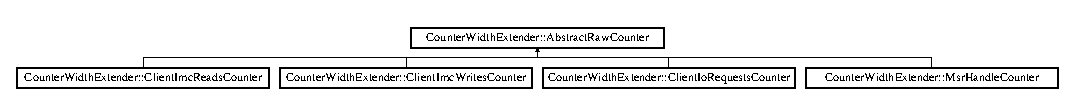
\includegraphics[height=0.968858cm]{structCounterWidthExtender_1_1AbstractRawCounter}
\end{center}
\end{figure}
\subsection*{Public Member Functions}
\begin{DoxyCompactItemize}
\item 
virtual uint64 {\bfseries operator()} ()=0\label{structCounterWidthExtender_1_1AbstractRawCounter_a608ae097b3e1fd42768f3cd408fa123d}

\end{DoxyCompactItemize}


The documentation for this struct was generated from the following file\+:\begin{DoxyCompactItemize}
\item 
{\bf width\+\_\+extender.\+h}\end{DoxyCompactItemize}

\section{Asynchron\+Counter\+State Class Reference}
\label{classAsynchronCounterState}\index{Asynchron\+Counter\+State@{Asynchron\+Counter\+State}}
\subsection*{Public Member Functions}
\begin{DoxyCompactItemize}
\item 
uint32 {\bfseries get\+Num\+Cores} ()\label{classAsynchronCounterState_ae50ebd3674b3ba52ff25f46b4eeb3956}

\item 
uint32 {\bfseries get\+Num\+Sockets} ()\label{classAsynchronCounterState_aad5f8ed144ee05d32c4b82e8664ea294}

\item 
uint32 {\bfseries get\+Q\+P\+I\+Links\+Per\+Socket} ()\label{classAsynchronCounterState_ab221a101212adceb2a248691eca8db1a}

\item 
uint32 {\bfseries get\+Socket\+Id} (uint32 c)\label{classAsynchronCounterState_a9121ce142b39fd845f6c4eb101c214bf}

\item 
{\footnotesize template$<$typename T , T  func$>$ }\\{\bf T} {\bfseries get} (uint32 core)\label{classAsynchronCounterState_a8f8e4539b38c5f171faa235b196e6f6a}

\item 
{\footnotesize template$<$typename T , T  func$>$ }\\{\bf T} {\bfseries get} (int param, uint32 core)\label{classAsynchronCounterState_aa77c2086bbaa8214dc60176f6ba08e43}

\item 
{\footnotesize template$<$typename T , T  func$>$ }\\{\bf T} {\bfseries get\+Socket} (uint32 socket)\label{classAsynchronCounterState_a272fad1f3bd704f873c9c3a29e95192b}

\item 
{\footnotesize template$<$typename T , T  func$>$ }\\{\bf T} {\bfseries get\+Socket} (int param, uint32 socket)\label{classAsynchronCounterState_aba3224acb89e692bb7024c85a516b8cb}

\item 
{\footnotesize template$<$typename T , T  func$>$ }\\{\bf T} {\bfseries get\+Socket} (uint32 socket, uint32 param)\label{classAsynchronCounterState_ac5441bad9ff3aaccbe5b3b8965e091d2}

\item 
{\footnotesize template$<$typename T , T  func$>$ }\\{\bf T} {\bfseries get\+System} ()\label{classAsynchronCounterState_aa474d444ebe77a8c7e94c904e87879ae}

\item 
{\footnotesize template$<$typename T , T  func$>$ }\\{\bf T} {\bfseries get\+System} (int param)\label{classAsynchronCounterState_a689f439c1e0f3b68401a0dd4341b46f0}

\end{DoxyCompactItemize}
\subsection*{Friends}
\begin{DoxyCompactItemize}
\item 
void $\ast$ {\bfseries Update\+Counters} (void $\ast$)\label{classAsynchronCounterState_a972a576e955b250f38283c8c165a6c7a}

\end{DoxyCompactItemize}


The documentation for this class was generated from the following file\+:\begin{DoxyCompactItemize}
\item 
{\bf cpuasynchcounter.\+h}\end{DoxyCompactItemize}

\section{Basic\+Counter\+State Class Reference}
\label{classBasicCounterState}\index{Basic\+Counter\+State@{Basic\+Counter\+State}}


Basic core counter state.  




{\ttfamily \#include $<$cpucounters.\+h$>$}

Inheritance diagram for Basic\+Counter\+State\+:\begin{figure}[H]
\begin{center}
\leavevmode
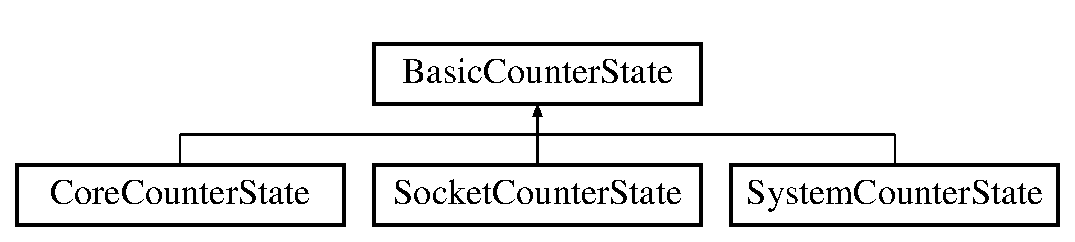
\includegraphics[height=2.000000cm]{classBasicCounterState}
\end{center}
\end{figure}
\subsection*{Public Member Functions}
\begin{DoxyCompactItemize}
\item 
{\bf Basic\+Counter\+State} \& {\bfseries operator+=} (const {\bf Basic\+Counter\+State} \&o)\label{classBasicCounterState_a448f898e8ff78336611db856aa1354db}

\item 
int32 {\bf get\+Thermal\+Headroom} () const \label{classBasicCounterState_a5411f6d468e66da3357a41f3c0fd1cb2}

\begin{DoxyCompactList}\small\item\em Returns current thermal headroom below Tj\+Max. \end{DoxyCompactList}\end{DoxyCompactItemize}
\subsection*{Protected Member Functions}
\begin{DoxyCompactItemize}
\item 
void {\bfseries read\+And\+Aggregate} ({\bf Safe\+Msr\+Handle} $\ast$)\label{classBasicCounterState_a1f983c45cc8e181dfee153a735afbe98}

\end{DoxyCompactItemize}
\subsection*{Protected Attributes}
\begin{DoxyCompactItemize}
\item 
uint64 {\bfseries Inst\+Retired\+Any}\label{classBasicCounterState_a32d89649ba3e48ad8d0cfe05b0e5e2fb}

\item 
uint64 {\bfseries Cpu\+Clk\+Unhalted\+Thread}\label{classBasicCounterState_aa55976b14e3f5d61eac958ea5f80f35c}

\item 
uint64 {\bfseries Cpu\+Clk\+Unhalted\+Ref}\label{classBasicCounterState_a9c64ac8f2c735b0a693a066ff99b9bc1}

\item 
\begin{tabbing}
xx\=xx\=xx\=xx\=xx\=xx\=xx\=xx\=xx\=\kill
union \{\\
\>uint64 {\bfseries L3Miss}\\
\>uint64 {\bfseries Event0}\\
\>uint64 {\bfseries ArchLLCMiss}\\
\}; \label{classBasicCounterState_a959ed48b231cadff965fa70acd60ade7}
\\

\end{tabbing}\item 
\begin{tabbing}
xx\=xx\=xx\=xx\=xx\=xx\=xx\=xx\=xx\=\kill
union \{\\
\>uint64 {\bfseries L3UnsharedHit}\\
\>uint64 {\bfseries Event1}\\
\>uint64 {\bfseries ArchLLCRef}\\
\}; \label{classBasicCounterState_a21d9f8b810e7625a425c469cd6fae52f}
\\

\end{tabbing}\item 
\begin{tabbing}
xx\=xx\=xx\=xx\=xx\=xx\=xx\=xx\=xx\=\kill
union \{\\
\>uint64 {\bfseries L2HitM}\\
\>uint64 {\bfseries Event2}\\
\}; \label{classBasicCounterState_a26f75e8ad60efecbdb155be81cc78ab8}
\\

\end{tabbing}\item 
\begin{tabbing}
xx\=xx\=xx\=xx\=xx\=xx\=xx\=xx\=xx\=\kill
union \{\\
\>uint64 {\bfseries L2Hit}\\
\>uint64 {\bfseries Event3}\\
\}; \label{classBasicCounterState_a4916830df8f468c47f33b7e9d66fdd22}
\\

\end{tabbing}\item 
uint64 {\bfseries Invariant\+T\+S\+C}\label{classBasicCounterState_af357162e5b43c6dfc0ce92fd56fa30a0}

\item 
uint64 {\bfseries C\+State\+Residency} [P\+C\+M\+::\+M\+A\+X\+\_\+\+C\+\_\+\+S\+T\+A\+T\+E+1]\label{classBasicCounterState_af9069c972052bac5ed648e519e03da9c}

\item 
int32 {\bfseries Thermal\+Headroom}\label{classBasicCounterState_a4950fe3761b2ac599a7ae64ec7bee973}

\item 
uint64 {\bfseries L3\+Occupancy}\label{classBasicCounterState_a99dab23e20418b86be72dda1ecd8858c}

\end{DoxyCompactItemize}
\subsection*{Friends}
\begin{DoxyCompactItemize}
\item 
class {\bfseries P\+C\+M}\label{classBasicCounterState_ab5f56d2e95ba3daf52c17b8a1d356d64}

\item 
{\footnotesize template$<$class Counter\+State\+Type $>$ }\\double {\bf get\+Exec\+Usage} (const Counter\+State\+Type \&before, const Counter\+State\+Type \&after)
\begin{DoxyCompactList}\small\item\em Computes average number of retired instructions per time intervall. \end{DoxyCompactList}\item 
{\footnotesize template$<$class Counter\+State\+Type $>$ }\\double {\bf get\+I\+P\+C} (const Counter\+State\+Type \&before, const Counter\+State\+Type \&after)
\begin{DoxyCompactList}\small\item\em Computes average number of retired instructions per core cycle (I\+P\+C) \end{DoxyCompactList}\item 
{\footnotesize template$<$class Counter\+State\+Type $>$ }\\double {\bf get\+Average\+Frequency} (const Counter\+State\+Type \&before, const Counter\+State\+Type \&after)
\begin{DoxyCompactList}\small\item\em Computes average core frequency also taking Intel Turbo Boost technology into account. \end{DoxyCompactList}\item 
{\footnotesize template$<$class Counter\+State\+Type $>$ }\\double {\bf get\+Active\+Average\+Frequency} (const Counter\+State\+Type \&before, const Counter\+State\+Type \&after)
\begin{DoxyCompactList}\small\item\em Computes average core frequency when not in powersaving C0-\/state (also taking Intel Turbo Boost technology into account) \end{DoxyCompactList}\item 
{\footnotesize template$<$class Counter\+State\+Type $>$ }\\double {\bf get\+Cycles\+Lost\+Due\+L3\+Cache\+Misses} (const Counter\+State\+Type \&before, const Counter\+State\+Type \&after)
\begin{DoxyCompactList}\small\item\em Estimates how many core cycles were potentially lost due to L3 cache misses. \end{DoxyCompactList}\item 
{\footnotesize template$<$class Counter\+State\+Type $>$ }\\double {\bf get\+Cycles\+Lost\+Due\+L2\+Cache\+Misses} (const Counter\+State\+Type \&before, const Counter\+State\+Type \&after)
\begin{DoxyCompactList}\small\item\em Estimates how many core cycles were potentially lost due to missing L2 cache but still hitting L3 cache. \end{DoxyCompactList}\item 
{\footnotesize template$<$class Counter\+State\+Type $>$ }\\double {\bf get\+Relative\+Frequency} (const Counter\+State\+Type \&before, const Counter\+State\+Type \&after)
\begin{DoxyCompactList}\small\item\em Computes average core frequency also taking Intel Turbo Boost technology into account. \end{DoxyCompactList}\item 
{\footnotesize template$<$class Counter\+State\+Type $>$ }\\double {\bf get\+Active\+Relative\+Frequency} (const Counter\+State\+Type \&before, const Counter\+State\+Type \&after)
\begin{DoxyCompactList}\small\item\em Computes average core frequency when not in powersaving C0-\/state (also taking Intel Turbo Boost technology into account) \end{DoxyCompactList}\item 
{\footnotesize template$<$class Counter\+State\+Type $>$ }\\double {\bf get\+L2\+Cache\+Hit\+Ratio} (const Counter\+State\+Type \&before, const Counter\+State\+Type \&after)
\begin{DoxyCompactList}\small\item\em Computes L2 cache hit ratio. \end{DoxyCompactList}\item 
{\footnotesize template$<$class Counter\+State\+Type $>$ }\\double {\bf get\+L3\+Cache\+Hit\+Ratio} (const Counter\+State\+Type \&before, const Counter\+State\+Type \&after)
\begin{DoxyCompactList}\small\item\em Computes L3 cache hit ratio. \end{DoxyCompactList}\item 
{\footnotesize template$<$class Counter\+State\+Type $>$ }\\uint64 {\bf get\+L3\+Cache\+Misses} (const Counter\+State\+Type \&before, const Counter\+State\+Type \&after)
\begin{DoxyCompactList}\small\item\em Computes number of L3 cache misses. \end{DoxyCompactList}\item 
{\footnotesize template$<$class Counter\+State\+Type $>$ }\\uint64 {\bf get\+L2\+Cache\+Misses} (const Counter\+State\+Type \&before, const Counter\+State\+Type \&after)
\begin{DoxyCompactList}\small\item\em Computes number of L2 cache misses. \end{DoxyCompactList}\item 
{\footnotesize template$<$class Counter\+State\+Type $>$ }\\uint64 {\bf get\+L2\+Cache\+Hits} (const Counter\+State\+Type \&before, const Counter\+State\+Type \&after)
\begin{DoxyCompactList}\small\item\em Computes number of L2 cache hits. \end{DoxyCompactList}\item 
{\footnotesize template$<$class Counter\+State\+Type $>$ }\\uint64 {\bf get\+L3\+Cache\+Occupancy} (const Counter\+State\+Type \&now)
\begin{DoxyCompactList}\small\item\em Computes L3 Cache Occupancy. \end{DoxyCompactList}\item 
{\footnotesize template$<$class Counter\+State\+Type $>$ }\\uint64 {\bf get\+Cycles} (const Counter\+State\+Type \&before, const Counter\+State\+Type \&after)
\begin{DoxyCompactList}\small\item\em Computes the number core clock cycles when signal on a specific core is running (not halted) \end{DoxyCompactList}\item 
{\footnotesize template$<$class Counter\+State\+Type $>$ }\\uint64 {\bf get\+Instructions\+Retired} (const Counter\+State\+Type \&before, const Counter\+State\+Type \&after)
\begin{DoxyCompactList}\small\item\em Computes the number of retired instructions. \end{DoxyCompactList}\item 
{\footnotesize template$<$class Counter\+State\+Type $>$ }\\uint64 {\bf get\+Cycles} (const Counter\+State\+Type \&now)
\begin{DoxyCompactList}\small\item\em Computes the number executed core clock cycles. \end{DoxyCompactList}\item 
{\footnotesize template$<$class Counter\+State\+Type $>$ }\\uint64 {\bf get\+Instructions\+Retired} (const Counter\+State\+Type \&now)
\begin{DoxyCompactList}\small\item\em Computes the number of retired instructions. \end{DoxyCompactList}\item 
{\footnotesize template$<$class Counter\+State\+Type $>$ }\\uint64 {\bf get\+L3\+Cache\+Hits\+No\+Snoop} (const Counter\+State\+Type \&before, const Counter\+State\+Type \&after)
\begin{DoxyCompactList}\small\item\em Computes number of L3 cache hits where no snooping in sibling L2 caches had to be done. \end{DoxyCompactList}\item 
{\footnotesize template$<$class Counter\+State\+Type $>$ }\\uint64 {\bf get\+L3\+Cache\+Hits\+Snoop} (const Counter\+State\+Type \&before, const Counter\+State\+Type \&after)
\begin{DoxyCompactList}\small\item\em Computes number of L3 cache hits where snooping in sibling L2 caches had to be done. \end{DoxyCompactList}\item 
{\footnotesize template$<$class Counter\+State\+Type $>$ }\\uint64 {\bf get\+L3\+Cache\+Hits} (const Counter\+State\+Type \&before, const Counter\+State\+Type \&after)
\begin{DoxyCompactList}\small\item\em Computes total number of L3 cache hits. \end{DoxyCompactList}\item 
{\footnotesize template$<$class Counter\+State\+Type $>$ }\\uint64 {\bf get\+Number\+Of\+Custom\+Events} (int32 event\+Counter\+Nr, const Counter\+State\+Type \&before, const Counter\+State\+Type \&after)
\begin{DoxyCompactList}\small\item\em Returns the number of occured custom core events. \end{DoxyCompactList}\item 
{\footnotesize template$<$class Counter\+State\+Type $>$ }\\uint64 {\bf get\+Invariant\+T\+S\+C} (const Counter\+State\+Type \&before, const Counter\+State\+Type \&after)
\begin{DoxyCompactList}\small\item\em Computes number of invariant time stamp counter ticks. \end{DoxyCompactList}\item 
{\footnotesize template$<$class Counter\+State\+Type $>$ }\\uint64 {\bf get\+Ref\+Cycles} (const Counter\+State\+Type \&before, const Counter\+State\+Type \&after)
\begin{DoxyCompactList}\small\item\em Computes the number of reference clock cycles while clock signal on the core is running. \end{DoxyCompactList}\item 
{\footnotesize template$<$class Counter\+State\+Type $>$ }\\double {\bf get\+Core\+C\+State\+Residency} (int state, const Counter\+State\+Type \&before, const Counter\+State\+Type \&after)
\begin{DoxyCompactList}\small\item\em Computes residency in the core C-\/state. \end{DoxyCompactList}\end{DoxyCompactItemize}


\subsection{Detailed Description}
Basic core counter state. 

Intended only for derivation, but not for the direct use 

\subsection{Friends And Related Function Documentation}
\index{Basic\+Counter\+State@{Basic\+Counter\+State}!get\+Active\+Average\+Frequency@{get\+Active\+Average\+Frequency}}
\index{get\+Active\+Average\+Frequency@{get\+Active\+Average\+Frequency}!Basic\+Counter\+State@{Basic\+Counter\+State}}
\subsubsection[{get\+Active\+Average\+Frequency}]{\setlength{\rightskip}{0pt plus 5cm}template$<$class Counter\+State\+Type $>$ double get\+Active\+Average\+Frequency (
\begin{DoxyParamCaption}
\item[{const Counter\+State\+Type \&}]{before, }
\item[{const Counter\+State\+Type \&}]{after}
\end{DoxyParamCaption}
)\hspace{0.3cm}{\ttfamily [friend]}}\label{classBasicCounterState_a963d78be64ccddb4f7686405ef4df9c1}


Computes average core frequency when not in powersaving C0-\/state (also taking Intel Turbo Boost technology into account) 


\begin{DoxyParams}{Parameters}
{\em before} & C\+P\+U counter state before the experiment \\
\hline
{\em after} & C\+P\+U counter state after the experiment \\
\hline
\end{DoxyParams}
\begin{DoxyReturn}{Returns}
frequency in Hz 
\end{DoxyReturn}
\index{Basic\+Counter\+State@{Basic\+Counter\+State}!get\+Active\+Relative\+Frequency@{get\+Active\+Relative\+Frequency}}
\index{get\+Active\+Relative\+Frequency@{get\+Active\+Relative\+Frequency}!Basic\+Counter\+State@{Basic\+Counter\+State}}
\subsubsection[{get\+Active\+Relative\+Frequency}]{\setlength{\rightskip}{0pt plus 5cm}template$<$class Counter\+State\+Type $>$ double get\+Active\+Relative\+Frequency (
\begin{DoxyParamCaption}
\item[{const Counter\+State\+Type \&}]{before, }
\item[{const Counter\+State\+Type \&}]{after}
\end{DoxyParamCaption}
)\hspace{0.3cm}{\ttfamily [friend]}}\label{classBasicCounterState_a9a351e598b8af26131611ff37b592633}


Computes average core frequency when not in powersaving C0-\/state (also taking Intel Turbo Boost technology into account) 


\begin{DoxyParams}{Parameters}
{\em before} & C\+P\+U counter state before the experiment \\
\hline
{\em after} & C\+P\+U counter state after the experiment \\
\hline
\end{DoxyParams}
\begin{DoxyReturn}{Returns}
Fraction of nominal frequency (if $>$1.\+0 then Turbo was working during the measurement) 
\end{DoxyReturn}
\index{Basic\+Counter\+State@{Basic\+Counter\+State}!get\+Average\+Frequency@{get\+Average\+Frequency}}
\index{get\+Average\+Frequency@{get\+Average\+Frequency}!Basic\+Counter\+State@{Basic\+Counter\+State}}
\subsubsection[{get\+Average\+Frequency}]{\setlength{\rightskip}{0pt plus 5cm}template$<$class Counter\+State\+Type $>$ double get\+Average\+Frequency (
\begin{DoxyParamCaption}
\item[{const Counter\+State\+Type \&}]{before, }
\item[{const Counter\+State\+Type \&}]{after}
\end{DoxyParamCaption}
)\hspace{0.3cm}{\ttfamily [friend]}}\label{classBasicCounterState_aa398facfd523b7dcdbf827a74970a88c}


Computes average core frequency also taking Intel Turbo Boost technology into account. 


\begin{DoxyParams}{Parameters}
{\em before} & C\+P\+U counter state before the experiment \\
\hline
{\em after} & C\+P\+U counter state after the experiment \\
\hline
\end{DoxyParams}
\begin{DoxyReturn}{Returns}
frequency in Hz 
\end{DoxyReturn}
\index{Basic\+Counter\+State@{Basic\+Counter\+State}!get\+Core\+C\+State\+Residency@{get\+Core\+C\+State\+Residency}}
\index{get\+Core\+C\+State\+Residency@{get\+Core\+C\+State\+Residency}!Basic\+Counter\+State@{Basic\+Counter\+State}}
\subsubsection[{get\+Core\+C\+State\+Residency}]{\setlength{\rightskip}{0pt plus 5cm}template$<$class Counter\+State\+Type $>$ double get\+Core\+C\+State\+Residency (
\begin{DoxyParamCaption}
\item[{int}]{state, }
\item[{const Counter\+State\+Type \&}]{before, }
\item[{const Counter\+State\+Type \&}]{after}
\end{DoxyParamCaption}
)\hspace{0.3cm}{\ttfamily [friend]}}\label{classBasicCounterState_a98aa8d4eb21e8a992fc181d65018e5ce}


Computes residency in the core C-\/state. 


\begin{DoxyParams}{Parameters}
{\em state} & C-\/state \\
\hline
{\em before} & C\+P\+U counter state before the experiment \\
\hline
{\em after} & C\+P\+U counter state after the experiment \\
\hline
\end{DoxyParams}
\begin{DoxyReturn}{Returns}
residence ratio (0..1)\+: 0 -\/ 0\%, 1.\+0 -\/ 100\% 
\end{DoxyReturn}
\index{Basic\+Counter\+State@{Basic\+Counter\+State}!get\+Cycles@{get\+Cycles}}
\index{get\+Cycles@{get\+Cycles}!Basic\+Counter\+State@{Basic\+Counter\+State}}
\subsubsection[{get\+Cycles}]{\setlength{\rightskip}{0pt plus 5cm}template$<$class Counter\+State\+Type $>$ uint64 get\+Cycles (
\begin{DoxyParamCaption}
\item[{const Counter\+State\+Type \&}]{before, }
\item[{const Counter\+State\+Type \&}]{after}
\end{DoxyParamCaption}
)\hspace{0.3cm}{\ttfamily [friend]}}\label{classBasicCounterState_a5a3275c4f489a475f1658f4546567af4}


Computes the number core clock cycles when signal on a specific core is running (not halted) 

Returns number of used cycles (halted cyles are not counted). The counter does not advance in the following conditions\+:
\begin{DoxyItemize}
\item an A\+C\+P\+I C-\/state is other than C0 for normal operation
\item H\+L\+T
\item S\+T\+P\+C\+L\+K+ pin is asserted
\item being throttled by T\+M1
\item during the frequency switching phase of a performance state transition
\end{DoxyItemize}

The performance counter for this event counts across performance state transitions using different core clock frequencies


\begin{DoxyParams}{Parameters}
{\em before} & C\+P\+U counter state before the experiment \\
\hline
{\em after} & C\+P\+U counter state after the experiment \\
\hline
\end{DoxyParams}
\begin{DoxyReturn}{Returns}
number core clock cycles 
\end{DoxyReturn}
\index{Basic\+Counter\+State@{Basic\+Counter\+State}!get\+Cycles@{get\+Cycles}}
\index{get\+Cycles@{get\+Cycles}!Basic\+Counter\+State@{Basic\+Counter\+State}}
\subsubsection[{get\+Cycles}]{\setlength{\rightskip}{0pt plus 5cm}template$<$class Counter\+State\+Type $>$ uint64 get\+Cycles (
\begin{DoxyParamCaption}
\item[{const Counter\+State\+Type \&}]{now}
\end{DoxyParamCaption}
)\hspace{0.3cm}{\ttfamily [friend]}}\label{classBasicCounterState_adc17d576ecaf02cf98cebc86329bf2a1}


Computes the number executed core clock cycles. 

Returns number of used cycles (halted cyles are not counted).


\begin{DoxyParams}{Parameters}
{\em now} & Current C\+P\+U counter state \\
\hline
\end{DoxyParams}
\begin{DoxyReturn}{Returns}
number core clock cycles 
\end{DoxyReturn}
\index{Basic\+Counter\+State@{Basic\+Counter\+State}!get\+Cycles\+Lost\+Due\+L2\+Cache\+Misses@{get\+Cycles\+Lost\+Due\+L2\+Cache\+Misses}}
\index{get\+Cycles\+Lost\+Due\+L2\+Cache\+Misses@{get\+Cycles\+Lost\+Due\+L2\+Cache\+Misses}!Basic\+Counter\+State@{Basic\+Counter\+State}}
\subsubsection[{get\+Cycles\+Lost\+Due\+L2\+Cache\+Misses}]{\setlength{\rightskip}{0pt plus 5cm}template$<$class Counter\+State\+Type $>$ double get\+Cycles\+Lost\+Due\+L2\+Cache\+Misses (
\begin{DoxyParamCaption}
\item[{const Counter\+State\+Type \&}]{before, }
\item[{const Counter\+State\+Type \&}]{after}
\end{DoxyParamCaption}
)\hspace{0.3cm}{\ttfamily [friend]}}\label{classBasicCounterState_ac26765efe8a4c7341f40c8ab8bdb9af6}


Estimates how many core cycles were potentially lost due to missing L2 cache but still hitting L3 cache. 


\begin{DoxyParams}{Parameters}
{\em before} & C\+P\+U counter state before the experiment \\
\hline
{\em after} & C\+P\+U counter state after the experiment \\
\hline
\end{DoxyParams}
\begin{DoxyWarning}{Warning}
Works only in the D\+E\+F\+A\+U\+L\+T\+\_\+\+E\+V\+E\+N\+T\+S programming mode (see program() method) 

Currently not supported on Intel(\+R) Atom(tm) processor 
\end{DoxyWarning}
\begin{DoxyReturn}{Returns}
ratio that is usually beetween 0 and 1 ; in some cases could be $>$1.\+0 due to a lower access latency estimation 
\end{DoxyReturn}
\index{Basic\+Counter\+State@{Basic\+Counter\+State}!get\+Cycles\+Lost\+Due\+L3\+Cache\+Misses@{get\+Cycles\+Lost\+Due\+L3\+Cache\+Misses}}
\index{get\+Cycles\+Lost\+Due\+L3\+Cache\+Misses@{get\+Cycles\+Lost\+Due\+L3\+Cache\+Misses}!Basic\+Counter\+State@{Basic\+Counter\+State}}
\subsubsection[{get\+Cycles\+Lost\+Due\+L3\+Cache\+Misses}]{\setlength{\rightskip}{0pt plus 5cm}template$<$class Counter\+State\+Type $>$ double get\+Cycles\+Lost\+Due\+L3\+Cache\+Misses (
\begin{DoxyParamCaption}
\item[{const Counter\+State\+Type \&}]{before, }
\item[{const Counter\+State\+Type \&}]{after}
\end{DoxyParamCaption}
)\hspace{0.3cm}{\ttfamily [friend]}}\label{classBasicCounterState_a89d4cef9c83db7e76be6a0a2e7351e2e}


Estimates how many core cycles were potentially lost due to L3 cache misses. 


\begin{DoxyParams}{Parameters}
{\em before} & C\+P\+U counter state before the experiment \\
\hline
{\em after} & C\+P\+U counter state after the experiment \\
\hline
\end{DoxyParams}
\begin{DoxyWarning}{Warning}
Works only in the D\+E\+F\+A\+U\+L\+T\+\_\+\+E\+V\+E\+N\+T\+S programming mode (see program() method) 
\end{DoxyWarning}
\begin{DoxyReturn}{Returns}
ratio that is usually beetween 0 and 1 ; in some cases could be $>$1.\+0 due to a lower memory latency estimation 
\end{DoxyReturn}
\index{Basic\+Counter\+State@{Basic\+Counter\+State}!get\+Exec\+Usage@{get\+Exec\+Usage}}
\index{get\+Exec\+Usage@{get\+Exec\+Usage}!Basic\+Counter\+State@{Basic\+Counter\+State}}
\subsubsection[{get\+Exec\+Usage}]{\setlength{\rightskip}{0pt plus 5cm}template$<$class Counter\+State\+Type $>$ double get\+Exec\+Usage (
\begin{DoxyParamCaption}
\item[{const Counter\+State\+Type \&}]{before, }
\item[{const Counter\+State\+Type \&}]{after}
\end{DoxyParamCaption}
)\hspace{0.3cm}{\ttfamily [friend]}}\label{classBasicCounterState_a159a6896f5ef3626b88cdd27a3c15ac0}


Computes average number of retired instructions per time intervall. 


\begin{DoxyParams}{Parameters}
{\em before} & C\+P\+U counter state before the experiment \\
\hline
{\em after} & C\+P\+U counter state after the experiment \\
\hline
\end{DoxyParams}
\begin{DoxyReturn}{Returns}
usage 
\end{DoxyReturn}
\index{Basic\+Counter\+State@{Basic\+Counter\+State}!get\+Instructions\+Retired@{get\+Instructions\+Retired}}
\index{get\+Instructions\+Retired@{get\+Instructions\+Retired}!Basic\+Counter\+State@{Basic\+Counter\+State}}
\subsubsection[{get\+Instructions\+Retired}]{\setlength{\rightskip}{0pt plus 5cm}template$<$class Counter\+State\+Type $>$ uint64 get\+Instructions\+Retired (
\begin{DoxyParamCaption}
\item[{const Counter\+State\+Type \&}]{before, }
\item[{const Counter\+State\+Type \&}]{after}
\end{DoxyParamCaption}
)\hspace{0.3cm}{\ttfamily [friend]}}\label{classBasicCounterState_af124718a7620c7bbca81232c2149f771}


Computes the number of retired instructions. 


\begin{DoxyParams}{Parameters}
{\em before} & C\+P\+U counter state before the experiment \\
\hline
{\em after} & C\+P\+U counter state after the experiment \\
\hline
\end{DoxyParams}
\begin{DoxyReturn}{Returns}
number of retired instructions 
\end{DoxyReturn}
\index{Basic\+Counter\+State@{Basic\+Counter\+State}!get\+Instructions\+Retired@{get\+Instructions\+Retired}}
\index{get\+Instructions\+Retired@{get\+Instructions\+Retired}!Basic\+Counter\+State@{Basic\+Counter\+State}}
\subsubsection[{get\+Instructions\+Retired}]{\setlength{\rightskip}{0pt plus 5cm}template$<$class Counter\+State\+Type $>$ uint64 get\+Instructions\+Retired (
\begin{DoxyParamCaption}
\item[{const Counter\+State\+Type \&}]{now}
\end{DoxyParamCaption}
)\hspace{0.3cm}{\ttfamily [friend]}}\label{classBasicCounterState_afced47e4bb3712da79dc64cb16ac335a}


Computes the number of retired instructions. 


\begin{DoxyParams}{Parameters}
{\em now} & Current C\+P\+U counter state \\
\hline
\end{DoxyParams}
\begin{DoxyReturn}{Returns}
number of retired instructions 
\end{DoxyReturn}
\index{Basic\+Counter\+State@{Basic\+Counter\+State}!get\+Invariant\+T\+S\+C@{get\+Invariant\+T\+S\+C}}
\index{get\+Invariant\+T\+S\+C@{get\+Invariant\+T\+S\+C}!Basic\+Counter\+State@{Basic\+Counter\+State}}
\subsubsection[{get\+Invariant\+T\+S\+C}]{\setlength{\rightskip}{0pt plus 5cm}template$<$class Counter\+State\+Type $>$ uint64 get\+Invariant\+T\+S\+C (
\begin{DoxyParamCaption}
\item[{const Counter\+State\+Type \&}]{before, }
\item[{const Counter\+State\+Type \&}]{after}
\end{DoxyParamCaption}
)\hspace{0.3cm}{\ttfamily [friend]}}\label{classBasicCounterState_a45cf07a8d3ce2c48968842554a3854f9}


Computes number of invariant time stamp counter ticks. 

This counter counts irrespectively of C-\/, P-\/ or T-\/states


\begin{DoxyParams}{Parameters}
{\em before} & C\+P\+U counter state before the experiment \\
\hline
{\em after} & C\+P\+U counter state after the experiment \\
\hline
\end{DoxyParams}
\begin{DoxyReturn}{Returns}
number of time stamp counter ticks 
\end{DoxyReturn}
\index{Basic\+Counter\+State@{Basic\+Counter\+State}!get\+I\+P\+C@{get\+I\+P\+C}}
\index{get\+I\+P\+C@{get\+I\+P\+C}!Basic\+Counter\+State@{Basic\+Counter\+State}}
\subsubsection[{get\+I\+P\+C}]{\setlength{\rightskip}{0pt plus 5cm}template$<$class Counter\+State\+Type $>$ double get\+I\+P\+C (
\begin{DoxyParamCaption}
\item[{const Counter\+State\+Type \&}]{before, }
\item[{const Counter\+State\+Type \&}]{after}
\end{DoxyParamCaption}
)\hspace{0.3cm}{\ttfamily [friend]}}\label{classBasicCounterState_a7b0019d24a77dc05b7e47cb98192fd22}


Computes average number of retired instructions per core cycle (I\+P\+C) 


\begin{DoxyParams}{Parameters}
{\em before} & C\+P\+U counter state before the experiment \\
\hline
{\em after} & C\+P\+U counter state after the experiment \\
\hline
\end{DoxyParams}
\begin{DoxyReturn}{Returns}
I\+P\+C 
\end{DoxyReturn}
\index{Basic\+Counter\+State@{Basic\+Counter\+State}!get\+L2\+Cache\+Hit\+Ratio@{get\+L2\+Cache\+Hit\+Ratio}}
\index{get\+L2\+Cache\+Hit\+Ratio@{get\+L2\+Cache\+Hit\+Ratio}!Basic\+Counter\+State@{Basic\+Counter\+State}}
\subsubsection[{get\+L2\+Cache\+Hit\+Ratio}]{\setlength{\rightskip}{0pt plus 5cm}template$<$class Counter\+State\+Type $>$ double get\+L2\+Cache\+Hit\+Ratio (
\begin{DoxyParamCaption}
\item[{const Counter\+State\+Type \&}]{before, }
\item[{const Counter\+State\+Type \&}]{after}
\end{DoxyParamCaption}
)\hspace{0.3cm}{\ttfamily [friend]}}\label{classBasicCounterState_a5922acedeec3c1cc67d20670f8ef0518}


Computes L2 cache hit ratio. 


\begin{DoxyParams}{Parameters}
{\em before} & C\+P\+U counter state before the experiment \\
\hline
{\em after} & C\+P\+U counter state after the experiment \\
\hline
\end{DoxyParams}
\begin{DoxyWarning}{Warning}
Works only in the D\+E\+F\+A\+U\+L\+T\+\_\+\+E\+V\+E\+N\+T\+S programming mode (see program() method) 
\end{DoxyWarning}
\begin{DoxyReturn}{Returns}
value between 0 and 1 
\end{DoxyReturn}
\index{Basic\+Counter\+State@{Basic\+Counter\+State}!get\+L2\+Cache\+Hits@{get\+L2\+Cache\+Hits}}
\index{get\+L2\+Cache\+Hits@{get\+L2\+Cache\+Hits}!Basic\+Counter\+State@{Basic\+Counter\+State}}
\subsubsection[{get\+L2\+Cache\+Hits}]{\setlength{\rightskip}{0pt plus 5cm}template$<$class Counter\+State\+Type $>$ uint64 get\+L2\+Cache\+Hits (
\begin{DoxyParamCaption}
\item[{const Counter\+State\+Type \&}]{before, }
\item[{const Counter\+State\+Type \&}]{after}
\end{DoxyParamCaption}
)\hspace{0.3cm}{\ttfamily [friend]}}\label{classBasicCounterState_a459367d7877d09594c2ecd85e04cae61}


Computes number of L2 cache hits. 


\begin{DoxyParams}{Parameters}
{\em before} & C\+P\+U counter state before the experiment \\
\hline
{\em after} & C\+P\+U counter state after the experiment \\
\hline
\end{DoxyParams}
\begin{DoxyWarning}{Warning}
Works only in the D\+E\+F\+A\+U\+L\+T\+\_\+\+E\+V\+E\+N\+T\+S programming mode (see program() method) 
\end{DoxyWarning}
\begin{DoxyReturn}{Returns}
number of hits 
\end{DoxyReturn}
\index{Basic\+Counter\+State@{Basic\+Counter\+State}!get\+L2\+Cache\+Misses@{get\+L2\+Cache\+Misses}}
\index{get\+L2\+Cache\+Misses@{get\+L2\+Cache\+Misses}!Basic\+Counter\+State@{Basic\+Counter\+State}}
\subsubsection[{get\+L2\+Cache\+Misses}]{\setlength{\rightskip}{0pt plus 5cm}template$<$class Counter\+State\+Type $>$ uint64 get\+L2\+Cache\+Misses (
\begin{DoxyParamCaption}
\item[{const Counter\+State\+Type \&}]{before, }
\item[{const Counter\+State\+Type \&}]{after}
\end{DoxyParamCaption}
)\hspace{0.3cm}{\ttfamily [friend]}}\label{classBasicCounterState_a291eeab262fdb93de08cdfdf50dbad58}


Computes number of L2 cache misses. 


\begin{DoxyParams}{Parameters}
{\em before} & C\+P\+U counter state before the experiment \\
\hline
{\em after} & C\+P\+U counter state after the experiment \\
\hline
\end{DoxyParams}
\begin{DoxyWarning}{Warning}
Works only in the D\+E\+F\+A\+U\+L\+T\+\_\+\+E\+V\+E\+N\+T\+S programming mode (see program() method) 
\end{DoxyWarning}
\begin{DoxyReturn}{Returns}
number of misses 
\end{DoxyReturn}
\index{Basic\+Counter\+State@{Basic\+Counter\+State}!get\+L3\+Cache\+Hit\+Ratio@{get\+L3\+Cache\+Hit\+Ratio}}
\index{get\+L3\+Cache\+Hit\+Ratio@{get\+L3\+Cache\+Hit\+Ratio}!Basic\+Counter\+State@{Basic\+Counter\+State}}
\subsubsection[{get\+L3\+Cache\+Hit\+Ratio}]{\setlength{\rightskip}{0pt plus 5cm}template$<$class Counter\+State\+Type $>$ double get\+L3\+Cache\+Hit\+Ratio (
\begin{DoxyParamCaption}
\item[{const Counter\+State\+Type \&}]{before, }
\item[{const Counter\+State\+Type \&}]{after}
\end{DoxyParamCaption}
)\hspace{0.3cm}{\ttfamily [friend]}}\label{classBasicCounterState_a7b03f0cd02862716d717e897032b7885}


Computes L3 cache hit ratio. 


\begin{DoxyParams}{Parameters}
{\em before} & C\+P\+U counter state before the experiment \\
\hline
{\em after} & C\+P\+U counter state after the experiment \\
\hline
\end{DoxyParams}
\begin{DoxyWarning}{Warning}
Works only in the D\+E\+F\+A\+U\+L\+T\+\_\+\+E\+V\+E\+N\+T\+S programming mode (see program() method) 
\end{DoxyWarning}
\begin{DoxyReturn}{Returns}
value between 0 and 1 
\end{DoxyReturn}
\index{Basic\+Counter\+State@{Basic\+Counter\+State}!get\+L3\+Cache\+Hits@{get\+L3\+Cache\+Hits}}
\index{get\+L3\+Cache\+Hits@{get\+L3\+Cache\+Hits}!Basic\+Counter\+State@{Basic\+Counter\+State}}
\subsubsection[{get\+L3\+Cache\+Hits}]{\setlength{\rightskip}{0pt plus 5cm}template$<$class Counter\+State\+Type $>$ uint64 get\+L3\+Cache\+Hits (
\begin{DoxyParamCaption}
\item[{const Counter\+State\+Type \&}]{before, }
\item[{const Counter\+State\+Type \&}]{after}
\end{DoxyParamCaption}
)\hspace{0.3cm}{\ttfamily [friend]}}\label{classBasicCounterState_a7ba16714ef7ed547ad8648cb5b9e52f6}


Computes total number of L3 cache hits. 


\begin{DoxyParams}{Parameters}
{\em before} & C\+P\+U counter state before the experiment \\
\hline
{\em after} & C\+P\+U counter state after the experiment \\
\hline
\end{DoxyParams}
\begin{DoxyWarning}{Warning}
Works only in the D\+E\+F\+A\+U\+L\+T\+\_\+\+E\+V\+E\+N\+T\+S programming mode (see program() method) 
\end{DoxyWarning}
\begin{DoxyReturn}{Returns}
number of hits 
\end{DoxyReturn}
\index{Basic\+Counter\+State@{Basic\+Counter\+State}!get\+L3\+Cache\+Hits\+No\+Snoop@{get\+L3\+Cache\+Hits\+No\+Snoop}}
\index{get\+L3\+Cache\+Hits\+No\+Snoop@{get\+L3\+Cache\+Hits\+No\+Snoop}!Basic\+Counter\+State@{Basic\+Counter\+State}}
\subsubsection[{get\+L3\+Cache\+Hits\+No\+Snoop}]{\setlength{\rightskip}{0pt plus 5cm}template$<$class Counter\+State\+Type $>$ uint64 get\+L3\+Cache\+Hits\+No\+Snoop (
\begin{DoxyParamCaption}
\item[{const Counter\+State\+Type \&}]{before, }
\item[{const Counter\+State\+Type \&}]{after}
\end{DoxyParamCaption}
)\hspace{0.3cm}{\ttfamily [friend]}}\label{classBasicCounterState_ace0e3ffc23c20d0eda7663cb7e4899a2}


Computes number of L3 cache hits where no snooping in sibling L2 caches had to be done. 


\begin{DoxyParams}{Parameters}
{\em before} & C\+P\+U counter state before the experiment \\
\hline
{\em after} & C\+P\+U counter state after the experiment \\
\hline
\end{DoxyParams}
\begin{DoxyWarning}{Warning}
Works only in the D\+E\+F\+A\+U\+L\+T\+\_\+\+E\+V\+E\+N\+T\+S programming mode (see program() method) 
\end{DoxyWarning}
\begin{DoxyReturn}{Returns}
number of hits 
\end{DoxyReturn}
\index{Basic\+Counter\+State@{Basic\+Counter\+State}!get\+L3\+Cache\+Hits\+Snoop@{get\+L3\+Cache\+Hits\+Snoop}}
\index{get\+L3\+Cache\+Hits\+Snoop@{get\+L3\+Cache\+Hits\+Snoop}!Basic\+Counter\+State@{Basic\+Counter\+State}}
\subsubsection[{get\+L3\+Cache\+Hits\+Snoop}]{\setlength{\rightskip}{0pt plus 5cm}template$<$class Counter\+State\+Type $>$ uint64 get\+L3\+Cache\+Hits\+Snoop (
\begin{DoxyParamCaption}
\item[{const Counter\+State\+Type \&}]{before, }
\item[{const Counter\+State\+Type \&}]{after}
\end{DoxyParamCaption}
)\hspace{0.3cm}{\ttfamily [friend]}}\label{classBasicCounterState_a4b1050ca9ccdd66661df556bab70fd0f}


Computes number of L3 cache hits where snooping in sibling L2 caches had to be done. 


\begin{DoxyParams}{Parameters}
{\em before} & C\+P\+U counter state before the experiment \\
\hline
{\em after} & C\+P\+U counter state after the experiment \\
\hline
\end{DoxyParams}
\begin{DoxyWarning}{Warning}
Works only in the D\+E\+F\+A\+U\+L\+T\+\_\+\+E\+V\+E\+N\+T\+S programming mode (see program() method) 
\end{DoxyWarning}
\begin{DoxyReturn}{Returns}
number of hits 
\end{DoxyReturn}
\index{Basic\+Counter\+State@{Basic\+Counter\+State}!get\+L3\+Cache\+Misses@{get\+L3\+Cache\+Misses}}
\index{get\+L3\+Cache\+Misses@{get\+L3\+Cache\+Misses}!Basic\+Counter\+State@{Basic\+Counter\+State}}
\subsubsection[{get\+L3\+Cache\+Misses}]{\setlength{\rightskip}{0pt plus 5cm}template$<$class Counter\+State\+Type $>$ uint64 get\+L3\+Cache\+Misses (
\begin{DoxyParamCaption}
\item[{const Counter\+State\+Type \&}]{before, }
\item[{const Counter\+State\+Type \&}]{after}
\end{DoxyParamCaption}
)\hspace{0.3cm}{\ttfamily [friend]}}\label{classBasicCounterState_a94118e70266db2ed7fc6b8b7b4e2c343}


Computes number of L3 cache misses. 


\begin{DoxyParams}{Parameters}
{\em before} & C\+P\+U counter state before the experiment \\
\hline
{\em after} & C\+P\+U counter state after the experiment \\
\hline
\end{DoxyParams}
\begin{DoxyWarning}{Warning}
Works only in the D\+E\+F\+A\+U\+L\+T\+\_\+\+E\+V\+E\+N\+T\+S programming mode (see program() method) 
\end{DoxyWarning}
\begin{DoxyReturn}{Returns}
number of misses 
\end{DoxyReturn}
\index{Basic\+Counter\+State@{Basic\+Counter\+State}!get\+L3\+Cache\+Occupancy@{get\+L3\+Cache\+Occupancy}}
\index{get\+L3\+Cache\+Occupancy@{get\+L3\+Cache\+Occupancy}!Basic\+Counter\+State@{Basic\+Counter\+State}}
\subsubsection[{get\+L3\+Cache\+Occupancy}]{\setlength{\rightskip}{0pt plus 5cm}template$<$class Counter\+State\+Type $>$ uint64 get\+L3\+Cache\+Occupancy (
\begin{DoxyParamCaption}
\item[{const Counter\+State\+Type \&}]{now}
\end{DoxyParamCaption}
)\hspace{0.3cm}{\ttfamily [friend]}}\label{classBasicCounterState_a185f850a9a753d9cf4deb8299261fd4c}


Computes L3 Cache Occupancy. 

\index{Basic\+Counter\+State@{Basic\+Counter\+State}!get\+Number\+Of\+Custom\+Events@{get\+Number\+Of\+Custom\+Events}}
\index{get\+Number\+Of\+Custom\+Events@{get\+Number\+Of\+Custom\+Events}!Basic\+Counter\+State@{Basic\+Counter\+State}}
\subsubsection[{get\+Number\+Of\+Custom\+Events}]{\setlength{\rightskip}{0pt plus 5cm}template$<$class Counter\+State\+Type $>$ uint64 get\+Number\+Of\+Custom\+Events (
\begin{DoxyParamCaption}
\item[{int32}]{event\+Counter\+Nr, }
\item[{const Counter\+State\+Type \&}]{before, }
\item[{const Counter\+State\+Type \&}]{after}
\end{DoxyParamCaption}
)\hspace{0.3cm}{\ttfamily [friend]}}\label{classBasicCounterState_abaa9d828b52f41866bf7dc8ff491a62e}


Returns the number of occured custom core events. 

Read number of events programmed with the {\ttfamily C\+U\+S\+T\+O\+M\+\_\+\+C\+O\+R\+E\+\_\+\+E\+V\+E\+N\+T\+S} 


\begin{DoxyParams}{Parameters}
{\em event\+Counter\+Nr} & Event/counter number (value from 0 to 3) \\
\hline
{\em before} & C\+P\+U counter state before the experiment \\
\hline
{\em after} & C\+P\+U counter state after the experiment \\
\hline
\end{DoxyParams}
\begin{DoxyReturn}{Returns}
Number of bytes 
\end{DoxyReturn}
\index{Basic\+Counter\+State@{Basic\+Counter\+State}!get\+Ref\+Cycles@{get\+Ref\+Cycles}}
\index{get\+Ref\+Cycles@{get\+Ref\+Cycles}!Basic\+Counter\+State@{Basic\+Counter\+State}}
\subsubsection[{get\+Ref\+Cycles}]{\setlength{\rightskip}{0pt plus 5cm}template$<$class Counter\+State\+Type $>$ uint64 get\+Ref\+Cycles (
\begin{DoxyParamCaption}
\item[{const Counter\+State\+Type \&}]{before, }
\item[{const Counter\+State\+Type \&}]{after}
\end{DoxyParamCaption}
)\hspace{0.3cm}{\ttfamily [friend]}}\label{classBasicCounterState_aaa3691b803702deec828d0d8d8a8f326}


Computes the number of reference clock cycles while clock signal on the core is running. 

The reference clock operates at a fixed frequency, irrespective of core frequency changes due to performance state transitions. See Intel(r) Software Developer\textquotesingle{}s Manual for more details


\begin{DoxyParams}{Parameters}
{\em before} & C\+P\+U counter state before the experiment \\
\hline
{\em after} & C\+P\+U counter state after the experiment \\
\hline
\end{DoxyParams}
\begin{DoxyReturn}{Returns}
number core clock cycles 
\end{DoxyReturn}
\index{Basic\+Counter\+State@{Basic\+Counter\+State}!get\+Relative\+Frequency@{get\+Relative\+Frequency}}
\index{get\+Relative\+Frequency@{get\+Relative\+Frequency}!Basic\+Counter\+State@{Basic\+Counter\+State}}
\subsubsection[{get\+Relative\+Frequency}]{\setlength{\rightskip}{0pt plus 5cm}template$<$class Counter\+State\+Type $>$ double get\+Relative\+Frequency (
\begin{DoxyParamCaption}
\item[{const Counter\+State\+Type \&}]{before, }
\item[{const Counter\+State\+Type \&}]{after}
\end{DoxyParamCaption}
)\hspace{0.3cm}{\ttfamily [friend]}}\label{classBasicCounterState_a806e72bc51f05acc4af0667ca3334242}


Computes average core frequency also taking Intel Turbo Boost technology into account. 


\begin{DoxyParams}{Parameters}
{\em before} & C\+P\+U counter state before the experiment \\
\hline
{\em after} & C\+P\+U counter state after the experiment \\
\hline
\end{DoxyParams}
\begin{DoxyReturn}{Returns}
Fraction of nominal frequency 
\end{DoxyReturn}


The documentation for this class was generated from the following files\+:\begin{DoxyCompactItemize}
\item 
{\bf cpucounters.\+h}\item 
{\bf cpucounters.\+cpp}\end{DoxyCompactItemize}

\section{Beckton\+Uncore\+P\+M\+U\+C\+N\+T\+C\+T\+L\+Register Struct Reference}
\label{structBecktonUncorePMUCNTCTLRegister}\index{Beckton\+Uncore\+P\+M\+U\+C\+N\+T\+C\+T\+L\+Register@{Beckton\+Uncore\+P\+M\+U\+C\+N\+T\+C\+T\+L\+Register}}
\subsection*{Public Attributes}
\begin{DoxyCompactItemize}
\item 
\begin{tabbing}
xx\=xx\=xx\=xx\=xx\=xx\=xx\=xx\=xx\=\kill
union \{\\
\>struct \{\\
\>\>uint64 {\bfseries en}: 1\\
\>\>uint64 {\bfseries pmi\_en}: 1\\
\>\>uint64 {\bfseries count\_mode}: 2\\
\>\>uint64 {\bfseries storage\_mode}: 2\\
\>\>uint64 {\bfseries wrap\_mode}: 1\\
\>\>uint64 {\bfseries flag\_mode}: 1\\
\>\>uint64 {\bfseries rsv1}: 1\\
\>\>uint64 {\bfseries inc\_sel}: 5\\
\>\>uint64 {\bfseries rsv2}: 5\\
\>\>uint64 {\bfseries set\_flag\_sel}: 3\\
\>\} {\bfseries fields}\\
\>uint64 {\bfseries value}\\
\}; \label{structBecktonUncorePMUCNTCTLRegister_a33cae53d33d55aadf24adf89ddbf4b62}
\\

\end{tabbing}\end{DoxyCompactItemize}


The documentation for this struct was generated from the following file\+:\begin{DoxyCompactItemize}
\item 
{\bf types.\+h}\end{DoxyCompactItemize}

\section{Beckton\+Uncore\+P\+M\+U\+Z\+D\+P\+C\+T\+L\+F\+V\+C\+Register Struct Reference}
\label{structBecktonUncorePMUZDPCTLFVCRegister}\index{Beckton\+Uncore\+P\+M\+U\+Z\+D\+P\+C\+T\+L\+F\+V\+C\+Register@{Beckton\+Uncore\+P\+M\+U\+Z\+D\+P\+C\+T\+L\+F\+V\+C\+Register}}
\subsection*{Public Attributes}
\begin{DoxyCompactItemize}
\item 
\begin{tabbing}
xx\=xx\=xx\=xx\=xx\=xx\=xx\=xx\=xx\=\kill
union \{\\
\>struct \{\\
\>\>uint64 {\bfseries fvid}: 5\\
\>\>uint64 {\bfseries bcmd}: 3\\
\>\>uint64 {\bfseries resp}: 3\\
\>\>uint64 {\bfseries evnt0}: 3\\
\>\>uint64 {\bfseries evnt1}: 3\\
\>\>uint64 {\bfseries evnt2}: 3\\
\>\>uint64 {\bfseries evnt3}: 3\\
\>\>uint64 {\bfseries pbox\_init\_err}: 1\\
\>\} {\bfseries fields}\\
\>struct \{\\
\>\>uint64 {\bfseries fvid}: 6\\
\>\>uint64 {\bfseries bcmd}: 3\\
\>\>uint64 {\bfseries resp}: 3\\
\>\>uint64 {\bfseries evnt0}: 3\\
\>\>uint64 {\bfseries evnt1}: 3\\
\>\>uint64 {\bfseries evnt2}: 3\\
\>\>uint64 {\bfseries evnt3}: 3\\
\>\>uint64 {\bfseries pbox\_init\_err}: 1\\
\>\} {\bfseries fields\_wsm}\\
\>uint64 {\bfseries value}\\
\}; \label{structBecktonUncorePMUZDPCTLFVCRegister_a92490cac0cda82bb90103a7f347cbfae}
\\

\end{tabbing}\end{DoxyCompactItemize}


The documentation for this struct was generated from the following file\+:\begin{DoxyCompactItemize}
\item 
{\bf types.\+h}\end{DoxyCompactItemize}

\section{Client\+B\+W Class Reference}
\label{classClientBW}\index{Client\+B\+W@{Client\+B\+W}}
\subsection*{Public Member Functions}
\begin{DoxyCompactItemize}
\item 
uint64 {\bfseries get\+Imc\+Reads} ()\label{classClientBW_adfd4220c06e62c3c3afe94d8388bcfe7}

\item 
uint64 {\bfseries get\+Imc\+Writes} ()\label{classClientBW_ad6ff206335be757c9de8fb732e66d2da}

\item 
uint64 {\bfseries get\+Io\+Requests} ()\label{classClientBW_acf0f1555e987641be5196312b89eb12b}

\end{DoxyCompactItemize}


The documentation for this class was generated from the following file\+:\begin{DoxyCompactItemize}
\item 
{\bf client\+\_\+bw.\+h}\end{DoxyCompactItemize}

\section{Counter\+Width\+Extender\+:\+:Client\+Imc\+Reads\+Counter Struct Reference}
\label{structCounterWidthExtender_1_1ClientImcReadsCounter}\index{Counter\+Width\+Extender\+::\+Client\+Imc\+Reads\+Counter@{Counter\+Width\+Extender\+::\+Client\+Imc\+Reads\+Counter}}
Inheritance diagram for Counter\+Width\+Extender\+:\+:Client\+Imc\+Reads\+Counter\+:\begin{figure}[H]
\begin{center}
\leavevmode
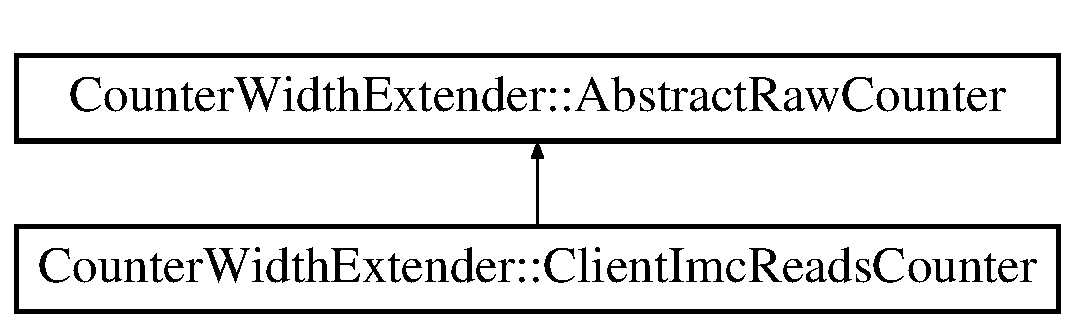
\includegraphics[height=2.000000cm]{structCounterWidthExtender_1_1ClientImcReadsCounter}
\end{center}
\end{figure}
\subsection*{Public Member Functions}
\begin{DoxyCompactItemize}
\item 
{\bfseries Client\+Imc\+Reads\+Counter} ({\bf Client\+B\+W} $\ast$client\+B\+W\+\_\+)\label{structCounterWidthExtender_1_1ClientImcReadsCounter_af716a073cdd4e2d027eb9f74ae6582a6}

\item 
uint64 {\bfseries operator()} ()\label{structCounterWidthExtender_1_1ClientImcReadsCounter_a2ce041afc601d13a4c19d75c2fae548f}

\end{DoxyCompactItemize}
\subsection*{Public Attributes}
\begin{DoxyCompactItemize}
\item 
{\bf Client\+B\+W} $\ast$ {\bfseries client\+B\+W}\label{structCounterWidthExtender_1_1ClientImcReadsCounter_a732e6a72ed34d60a3b55c949e7ed015e}

\end{DoxyCompactItemize}


The documentation for this struct was generated from the following file\+:\begin{DoxyCompactItemize}
\item 
{\bf width\+\_\+extender.\+h}\end{DoxyCompactItemize}

\section{Counter\+Width\+Extender\+:\+:Client\+Imc\+Writes\+Counter Struct Reference}
\label{structCounterWidthExtender_1_1ClientImcWritesCounter}\index{Counter\+Width\+Extender\+::\+Client\+Imc\+Writes\+Counter@{Counter\+Width\+Extender\+::\+Client\+Imc\+Writes\+Counter}}
Inheritance diagram for Counter\+Width\+Extender\+:\+:Client\+Imc\+Writes\+Counter\+:\begin{figure}[H]
\begin{center}
\leavevmode
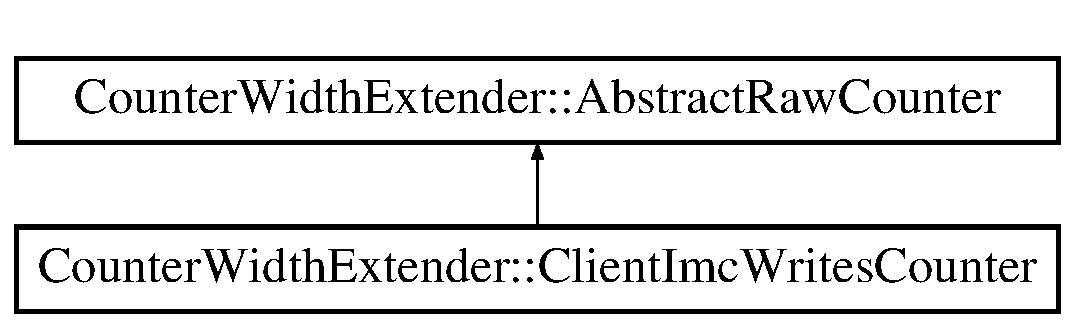
\includegraphics[height=2.000000cm]{structCounterWidthExtender_1_1ClientImcWritesCounter}
\end{center}
\end{figure}
\subsection*{Public Member Functions}
\begin{DoxyCompactItemize}
\item 
{\bfseries Client\+Imc\+Writes\+Counter} ({\bf Client\+B\+W} $\ast$client\+B\+W\+\_\+)\label{structCounterWidthExtender_1_1ClientImcWritesCounter_ac68fa6d6b3e258c2118bbb7ec401fbdd}

\item 
uint64 {\bfseries operator()} ()\label{structCounterWidthExtender_1_1ClientImcWritesCounter_a3156907cb67016aea3255b75d7a887cb}

\end{DoxyCompactItemize}
\subsection*{Public Attributes}
\begin{DoxyCompactItemize}
\item 
{\bf Client\+B\+W} $\ast$ {\bfseries client\+B\+W}\label{structCounterWidthExtender_1_1ClientImcWritesCounter_a1235306f7c8d86c962c373a0bce23c3c}

\end{DoxyCompactItemize}


The documentation for this struct was generated from the following file\+:\begin{DoxyCompactItemize}
\item 
{\bf width\+\_\+extender.\+h}\end{DoxyCompactItemize}

\section{Counter\+Width\+Extender\+:\+:Client\+Io\+Requests\+Counter Struct Reference}
\label{structCounterWidthExtender_1_1ClientIoRequestsCounter}\index{Counter\+Width\+Extender\+::\+Client\+Io\+Requests\+Counter@{Counter\+Width\+Extender\+::\+Client\+Io\+Requests\+Counter}}
Inheritance diagram for Counter\+Width\+Extender\+:\+:Client\+Io\+Requests\+Counter\+:\begin{figure}[H]
\begin{center}
\leavevmode
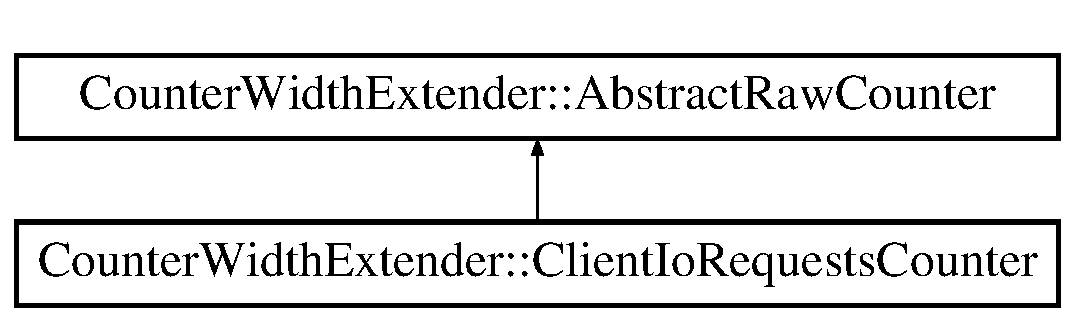
\includegraphics[height=2.000000cm]{structCounterWidthExtender_1_1ClientIoRequestsCounter}
\end{center}
\end{figure}
\subsection*{Public Member Functions}
\begin{DoxyCompactItemize}
\item 
{\bfseries Client\+Io\+Requests\+Counter} ({\bf Client\+B\+W} $\ast$client\+B\+W\+\_\+)\label{structCounterWidthExtender_1_1ClientIoRequestsCounter_a1a86c61304158b6504c502024b85330d}

\item 
uint64 {\bfseries operator()} ()\label{structCounterWidthExtender_1_1ClientIoRequestsCounter_a13cfbc3fedce8d039b306c303f485ff8}

\end{DoxyCompactItemize}
\subsection*{Public Attributes}
\begin{DoxyCompactItemize}
\item 
{\bf Client\+B\+W} $\ast$ {\bfseries client\+B\+W}\label{structCounterWidthExtender_1_1ClientIoRequestsCounter_ac76d8b2658c854c84be327c20f075e2b}

\end{DoxyCompactItemize}


The documentation for this struct was generated from the following file\+:\begin{DoxyCompactItemize}
\item 
{\bf width\+\_\+extender.\+h}\end{DoxyCompactItemize}

\section{Core\+Counter\+State Class Reference}
\label{classCoreCounterState}\index{Core\+Counter\+State@{Core\+Counter\+State}}


(Logical) core-\/wide counter state  




{\ttfamily \#include $<$cpucounters.\+h$>$}

Inheritance diagram for Core\+Counter\+State\+:\begin{figure}[H]
\begin{center}
\leavevmode
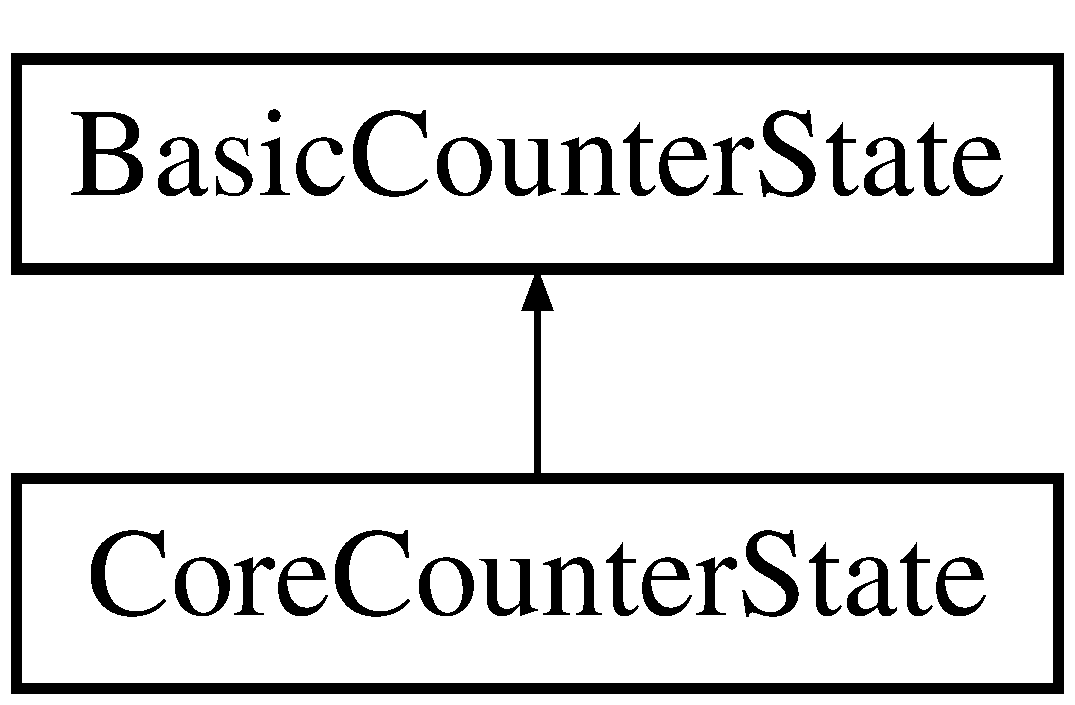
\includegraphics[height=2.000000cm]{classCoreCounterState}
\end{center}
\end{figure}
\subsection*{Friends}
\begin{DoxyCompactItemize}
\item 
class {\bfseries P\+C\+M}\label{classCoreCounterState_ab5f56d2e95ba3daf52c17b8a1d356d64}

\end{DoxyCompactItemize}
\subsection*{Additional Inherited Members}


\subsection{Detailed Description}
(Logical) core-\/wide counter state 

The documentation for this class was generated from the following file\+:\begin{DoxyCompactItemize}
\item 
{\bf cpucounters.\+h}\end{DoxyCompactItemize}

\section{Counter\+Width\+Extender Class Reference}
\label{classCounterWidthExtender}\index{Counter\+Width\+Extender@{Counter\+Width\+Extender}}
\subsection*{Classes}
\begin{DoxyCompactItemize}
\item 
struct {\bf Abstract\+Raw\+Counter}
\item 
struct {\bf Client\+Imc\+Reads\+Counter}
\item 
struct {\bf Client\+Imc\+Writes\+Counter}
\item 
struct {\bf Client\+Io\+Requests\+Counter}
\item 
struct {\bf Msr\+Handle\+Counter}
\end{DoxyCompactItemize}
\subsection*{Public Member Functions}
\begin{DoxyCompactItemize}
\item 
{\bfseries Counter\+Width\+Extender} ({\bf Abstract\+Raw\+Counter} $\ast$raw\+\_\+counter\+\_\+)\label{classCounterWidthExtender_a83aee7cbf9ba3f019181e025a953faf8}

\item 
uint64 {\bfseries read} ()\label{classCounterWidthExtender_a481ee1b6002b489711f7c8f2e17729f3}

\end{DoxyCompactItemize}


The documentation for this class was generated from the following file\+:\begin{DoxyCompactItemize}
\item 
{\bf width\+\_\+extender.\+h}\end{DoxyCompactItemize}

\section{P\+C\+M\+:\+:Custom\+Core\+Event\+Description Struct Reference}
\label{structPCM_1_1CustomCoreEventDescription}\index{P\+C\+M\+::\+Custom\+Core\+Event\+Description@{P\+C\+M\+::\+Custom\+Core\+Event\+Description}}


Custom Core event description.  




{\ttfamily \#include $<$cpucounters.\+h$>$}

\subsection*{Public Attributes}
\begin{DoxyCompactItemize}
\item 
int32 {\bfseries event\+\_\+number}\label{structPCM_1_1CustomCoreEventDescription_adfdbff9cf7c5be78450884b7adbd48fb}

\item 
int32 {\bfseries umask\+\_\+value}\label{structPCM_1_1CustomCoreEventDescription_a317a16603c27cf815fa62d88e7fd2f61}

\end{DoxyCompactItemize}


\subsection{Detailed Description}
Custom Core event description. 

See \char`\"{}\+Intel 64 and I\+A-\/32 Architectures Software Developers Manual Volume 3\+B\+:
\+System Programming Guide, Part 2\char`\"{} for the concrete values of the data structure fields, e.\+g. Appendix A.\+2 \char`\"{}\+Performance Monitoring Events for Intel(r) Core(tm) Processor Family
and Xeon Processor Family\char`\"{} 

The documentation for this struct was generated from the following file\+:\begin{DoxyCompactItemize}
\item 
{\bf cpucounters.\+h}\end{DoxyCompactItemize}

\section{Event\+Select\+Register Struct Reference}
\label{structEventSelectRegister}\index{Event\+Select\+Register@{Event\+Select\+Register}}
\subsection*{Public Attributes}
\begin{DoxyCompactItemize}
\item 
\begin{tabbing}
xx\=xx\=xx\=xx\=xx\=xx\=xx\=xx\=xx\=\kill
union \{\\
\>struct \{\\
\>\>uint64 {\bfseries event\_select}: 8\\
\>\>uint64 {\bfseries umask}: 8\\
\>\>uint64 {\bfseries usr}: 1\\
\>\>uint64 {\bfseries os}: 1\\
\>\>uint64 {\bfseries edge}: 1\\
\>\>uint64 {\bfseries pin\_control}: 1\\
\>\>uint64 {\bfseries apic\_int}: 1\\
\>\>uint64 {\bfseries any\_thread}: 1\\
\>\>uint64 {\bfseries enable}: 1\\
\>\>uint64 {\bfseries invert}: 1\\
\>\>uint64 {\bfseries cmask}: 8\\
\>\>uint64 {\bfseries in\_tx}: 1\\
\>\>uint64 {\bfseries in\_txcp}: 1\\
\>\>uint64 {\bfseries reservedX}: 30\\
\>\} {\bfseries fields}\\
\>uint64 {\bfseries value}\\
\}; \label{structEventSelectRegister_a86bb381e9495dec15d9489877b492db4}
\\

\end{tabbing}\end{DoxyCompactItemize}


The documentation for this struct was generated from the following file\+:\begin{DoxyCompactItemize}
\item 
{\bf types.\+h}\end{DoxyCompactItemize}

\section{P\+C\+M\+:\+:Extended\+Custom\+Core\+Event\+Description Struct Reference}
\label{structPCM_1_1ExtendedCustomCoreEventDescription}\index{P\+C\+M\+::\+Extended\+Custom\+Core\+Event\+Description@{P\+C\+M\+::\+Extended\+Custom\+Core\+Event\+Description}}


Extended custom core event description.  




{\ttfamily \#include $<$cpucounters.\+h$>$}

\subsection*{Public Attributes}
\begin{DoxyCompactItemize}
\item 
{\bf Fixed\+Event\+Control\+Register} $\ast$ {\bfseries fixed\+Cfg}\label{structPCM_1_1ExtendedCustomCoreEventDescription_a793e3dbd33a6bc37f800bb990777a543}

\item 
uint32 {\bfseries n\+G\+P\+Counters}\label{structPCM_1_1ExtendedCustomCoreEventDescription_ae66c1ea4e0b4ef493ee7d8c1f3245945}

\item 
{\bf Event\+Select\+Register} $\ast$ {\bfseries gp\+Counter\+Cfg}\label{structPCM_1_1ExtendedCustomCoreEventDescription_aa8f24e6871fe123345fd0141828374a1}

\item 
uint64 {\bfseries Offcore\+Response\+Msr\+Value} [2]\label{structPCM_1_1ExtendedCustomCoreEventDescription_a2a1a8771723138bddbeae034c7710934}

\end{DoxyCompactItemize}


\subsection{Detailed Description}
Extended custom core event description. 

In contrast to \doxyref{Custom\+Core\+Event\+Description}{p.}{structPCM_1_1CustomCoreEventDescription} supports configuration of all fields.

See \char`\"{}\+Intel 64 and I\+A-\/32 Architectures Software Developers Manual Volume 3\+B\+:
\+System Programming Guide, Part 2\char`\"{} for the concrete values of the data structure fields, e.\+g. Appendix A.\+2 \char`\"{}\+Performance Monitoring Events for Intel(r) Core(tm) Processor Family
and Xeon Processor Family\char`\"{} 

The documentation for this struct was generated from the following file\+:\begin{DoxyCompactItemize}
\item 
{\bf cpucounters.\+h}\end{DoxyCompactItemize}

\section{Fixed\+Event\+Control\+Register Struct Reference}
\label{structFixedEventControlRegister}\index{Fixed\+Event\+Control\+Register@{Fixed\+Event\+Control\+Register}}
\subsection*{Public Attributes}
\begin{DoxyCompactItemize}
\item 
\begin{tabbing}
xx\=xx\=xx\=xx\=xx\=xx\=xx\=xx\=xx\=\kill
union \{\\
\>struct \{\\
\>\>uint64 {\bfseries os0}: 1\\
\>\>uint64 {\bfseries usr0}: 1\\
\>\>uint64 {\bfseries any\_thread0}: 1\\
\>\>uint64 {\bfseries enable\_pmi0}: 1\\
\>\>uint64 {\bfseries os1}: 1\\
\>\>uint64 {\bfseries usr1}: 1\\
\>\>uint64 {\bfseries any\_thread1}: 1\\
\>\>uint64 {\bfseries enable\_pmi1}: 1\\
\>\>uint64 {\bfseries os2}: 1\\
\>\>uint64 {\bfseries usr2}: 1\\
\>\>uint64 {\bfseries any\_thread2}: 1\\
\>\>uint64 {\bfseries enable\_pmi2}: 1\\
\>\>uint64 {\bfseries reserved1}: 52\\
\>\} {\bfseries fields}\\
\>uint64 {\bfseries value}\\
\}; \label{structFixedEventControlRegister_a6e47972b5348979e8d53915444b7a150}
\\

\end{tabbing}\end{DoxyCompactItemize}


The documentation for this struct was generated from the following file\+:\begin{DoxyCompactItemize}
\item 
{\bf types.\+h}\end{DoxyCompactItemize}

\section{Instance\+Lock Class Reference}
\label{classInstanceLock}\index{Instance\+Lock@{Instance\+Lock}}
\subsection*{Public Member Functions}
\begin{DoxyCompactItemize}
\item 
{\bfseries Instance\+Lock} (const bool global\+\_\+)\label{classInstanceLock_a9fa936c0a79760e8fe4e93a7bee72cb1}

\end{DoxyCompactItemize}


The documentation for this class was generated from the following file\+:\begin{DoxyCompactItemize}
\item 
{\bf cpucounters.\+cpp}\end{DoxyCompactItemize}

\section{M\+C\+F\+G\+Header Struct Reference}
\label{structMCFGHeader}\index{M\+C\+F\+G\+Header@{M\+C\+F\+G\+Header}}
\subsection*{Public Member Functions}
\begin{DoxyCompactItemize}
\item 
unsigned {\bfseries nrecords} () const \label{structMCFGHeader_ad356ff2be2ef2c41613a7377ef831f4e}

\item 
void {\bfseries print} ()\label{structMCFGHeader_a3237441346fd64f80cb8b4b24aaa04cc}

\end{DoxyCompactItemize}
\subsection*{Public Attributes}
\begin{DoxyCompactItemize}
\item 
char {\bfseries signature} [4]\label{structMCFGHeader_a22b92d6805395592f50b9e9bc29e10df}

\item 
unsigned {\bfseries length}\label{structMCFGHeader_a621db3813e8b6b1fa6a19c061efbfd02}

\item 
unsigned char {\bfseries revision}\label{structMCFGHeader_a7f5a3f585900180ed744aa3a360beabf}

\item 
unsigned char {\bfseries checksum}\label{structMCFGHeader_ac4068aa15a9c7615a0b4b56c94317ad3}

\item 
char {\bfseries O\+E\+M\+I\+D} [6]\label{structMCFGHeader_a41f92a0973011550d26aff4f3b127d97}

\item 
char {\bfseries O\+E\+M\+Table\+I\+D} [8]\label{structMCFGHeader_ad3d67bd8da58f78fb582561c9b5780ab}

\item 
unsigned {\bfseries O\+E\+M\+Revision}\label{structMCFGHeader_ab27a08c03ed5ec7a0c22681089269c9a}

\item 
unsigned {\bfseries creator\+I\+D}\label{structMCFGHeader_af4ca343e759c3d8b1cc527d082d19ac0}

\item 
unsigned {\bfseries creator\+Revision}\label{structMCFGHeader_ada979c0affe38bf0c0c80f8de6356bb4}

\item 
char {\bfseries reserved} [8]\label{structMCFGHeader_ab705b7e929202f5876da9e0a6d474c7b}

\end{DoxyCompactItemize}


The documentation for this struct was generated from the following file\+:\begin{DoxyCompactItemize}
\item 
{\bf types.\+h}\end{DoxyCompactItemize}

\section{M\+C\+F\+G\+Record Struct Reference}
\label{structMCFGRecord}\index{M\+C\+F\+G\+Record@{M\+C\+F\+G\+Record}}
\subsection*{Public Member Functions}
\begin{DoxyCompactItemize}
\item 
void {\bfseries print} ()\label{structMCFGRecord_a4b954297f9dd2db580af3305dc2c1200}

\end{DoxyCompactItemize}
\subsection*{Public Attributes}
\begin{DoxyCompactItemize}
\item 
unsigned long long {\bfseries base\+Address}\label{structMCFGRecord_ab80de5ed728d89f1bd60647e0e909289}

\item 
unsigned short {\bfseries P\+C\+I\+Segment\+Group\+Number}\label{structMCFGRecord_a2ead77d33416e9f9a8607c7bdc9a3aa4}

\item 
unsigned char {\bfseries start\+Bus\+Number}\label{structMCFGRecord_a88a45ddf628776154cb5ed02b384061d}

\item 
unsigned char {\bfseries end\+Bus\+Number}\label{structMCFGRecord_a39692440cf50265f71b638d433a7ce37}

\item 
char {\bfseries reserved} [4]\label{structMCFGRecord_a549591813ff09495f6ee59cb3288f130}

\end{DoxyCompactItemize}


The documentation for this struct was generated from the following file\+:\begin{DoxyCompactItemize}
\item 
{\bf types.\+h}\end{DoxyCompactItemize}

\section{Msr\+Handle Class Reference}
\label{classMsrHandle}\index{Msr\+Handle@{Msr\+Handle}}
\subsection*{Public Member Functions}
\begin{DoxyCompactItemize}
\item 
{\bfseries Msr\+Handle} (uint32 cpu)\label{classMsrHandle_a481b0c81ad8f00d9d69db660e793a135}

\item 
int32 {\bfseries read} (uint64 msr\+\_\+number, uint64 $\ast$value)\label{classMsrHandle_a9a7723baaa1ec91a8303b5ef6579c1df}

\item 
int32 {\bfseries write} (uint64 msr\+\_\+number, uint64 value)\label{classMsrHandle_aa92da3c093ca1473eb7a7cad86f24c89}

\item 
int32 {\bfseries get\+Core\+Id} ()\label{classMsrHandle_adbbfac37adfdd3fb571b5a6978f60419}

\end{DoxyCompactItemize}


The documentation for this class was generated from the following files\+:\begin{DoxyCompactItemize}
\item 
{\bf msr.\+h}\item 
msr.\+cpp\end{DoxyCompactItemize}

\section{Counter\+Width\+Extender\+:\+:Msr\+Handle\+Counter Struct Reference}
\label{structCounterWidthExtender_1_1MsrHandleCounter}\index{Counter\+Width\+Extender\+::\+Msr\+Handle\+Counter@{Counter\+Width\+Extender\+::\+Msr\+Handle\+Counter}}
Inheritance diagram for Counter\+Width\+Extender\+:\+:Msr\+Handle\+Counter\+:\begin{figure}[H]
\begin{center}
\leavevmode
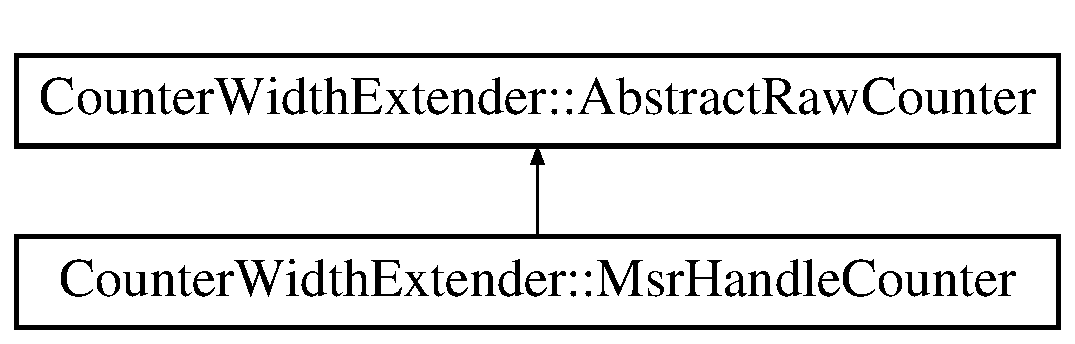
\includegraphics[height=2.000000cm]{structCounterWidthExtender_1_1MsrHandleCounter}
\end{center}
\end{figure}
\subsection*{Public Member Functions}
\begin{DoxyCompactItemize}
\item 
{\bfseries Msr\+Handle\+Counter} ({\bf Safe\+Msr\+Handle} $\ast$msr\+\_\+, uint64 msr\+\_\+addr\+\_\+)\label{structCounterWidthExtender_1_1MsrHandleCounter_a885cd6b474abacc975199541499e10cc}

\item 
uint64 {\bfseries operator()} ()\label{structCounterWidthExtender_1_1MsrHandleCounter_af6a1d4c47ab99efc52e87805b20457fc}

\end{DoxyCompactItemize}
\subsection*{Public Attributes}
\begin{DoxyCompactItemize}
\item 
{\bf Safe\+Msr\+Handle} $\ast$ {\bfseries msr}\label{structCounterWidthExtender_1_1MsrHandleCounter_a073583b253e413a52377f8a8f0f5a79b}

\item 
uint64 {\bfseries msr\+\_\+addr}\label{structCounterWidthExtender_1_1MsrHandleCounter_a5522d6a788192c2cb69b8d0c4fc0a9a1}

\end{DoxyCompactItemize}


The documentation for this struct was generated from the following file\+:\begin{DoxyCompactItemize}
\item 
{\bf width\+\_\+extender.\+h}\end{DoxyCompactItemize}

\section{null\+\_\+stream Struct Reference}
\label{structnull__stream}\index{null\+\_\+stream@{null\+\_\+stream}}
Inheritance diagram for null\+\_\+stream\+:\begin{figure}[H]
\begin{center}
\leavevmode
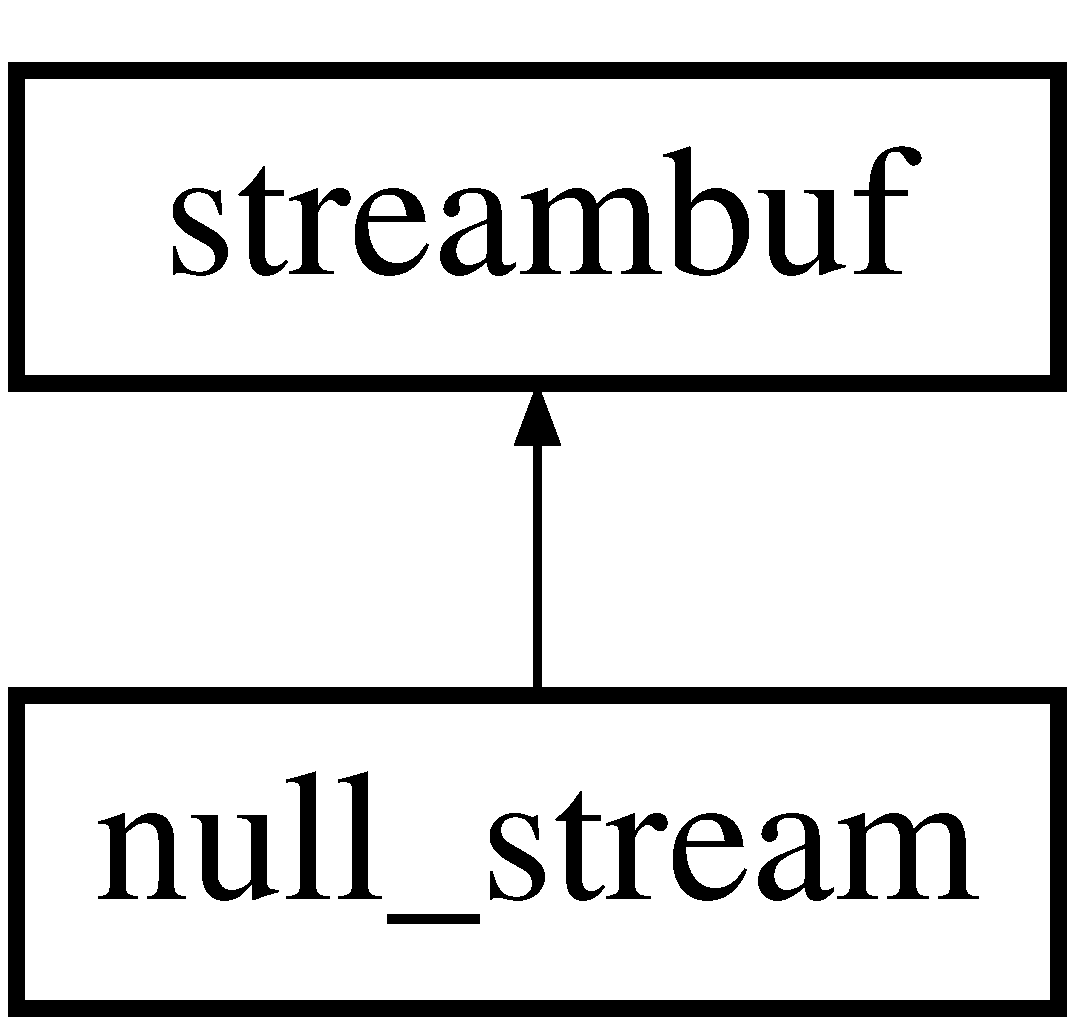
\includegraphics[height=2.000000cm]{structnull__stream}
\end{center}
\end{figure}
\subsection*{Public Member Functions}
\begin{DoxyCompactItemize}
\item 
void {\bfseries overflow} (char)\label{structnull__stream_a0bbaf9ee51c3dbe2583d3f2c0dfaeefb}

\end{DoxyCompactItemize}


The documentation for this struct was generated from the following file\+:\begin{DoxyCompactItemize}
\item 
{\bf utils.\+h}\end{DoxyCompactItemize}

\section{P\+C\+Ie\+Counter\+State Class Reference}
\label{classPCIeCounterState}\index{P\+C\+Ie\+Counter\+State@{P\+C\+Ie\+Counter\+State}}
\subsection*{Friends}
\begin{DoxyCompactItemize}
\item 
class {\bfseries P\+C\+M}\label{classPCIeCounterState_ab5f56d2e95ba3daf52c17b8a1d356d64}

\item 
uint64 {\bf get\+Number\+Of\+Events} ({\bf P\+C\+Ie\+Counter\+State} before, {\bf P\+C\+Ie\+Counter\+State} after)
\begin{DoxyCompactList}\small\item\em Returns the raw count of P\+C\+Ie events. \end{DoxyCompactList}\end{DoxyCompactItemize}


\subsection{Friends And Related Function Documentation}
\index{P\+C\+Ie\+Counter\+State@{P\+C\+Ie\+Counter\+State}!get\+Number\+Of\+Events@{get\+Number\+Of\+Events}}
\index{get\+Number\+Of\+Events@{get\+Number\+Of\+Events}!P\+C\+Ie\+Counter\+State@{P\+C\+Ie\+Counter\+State}}
\subsubsection[{get\+Number\+Of\+Events}]{\setlength{\rightskip}{0pt plus 5cm}uint64 get\+Number\+Of\+Events (
\begin{DoxyParamCaption}
\item[{{\bf P\+C\+Ie\+Counter\+State}}]{before, }
\item[{{\bf P\+C\+Ie\+Counter\+State}}]{after}
\end{DoxyParamCaption}
)\hspace{0.3cm}{\ttfamily [friend]}}\label{classPCIeCounterState_a3dfbc795387d801541439b6c035c7b8c}


Returns the raw count of P\+C\+Ie events. 


\begin{DoxyParams}{Parameters}
{\em before} & P\+C\+Ie counter state before the experiment \\
\hline
{\em after} & P\+C\+Ie counter state after the experiment \\
\hline
\end{DoxyParams}


The documentation for this class was generated from the following file\+:\begin{DoxyCompactItemize}
\item 
{\bf cpucounters.\+h}\end{DoxyCompactItemize}

\section{P\+C\+Ie\+Events\+\_\+t Struct Reference}
\label{structPCIeEvents__t}\index{P\+C\+Ie\+Events\+\_\+t@{P\+C\+Ie\+Events\+\_\+t}}
\subsection*{Public Attributes}
\begin{DoxyCompactItemize}
\item 
uint64 {\bfseries P\+C\+Ie\+Rd\+Cur}\label{structPCIeEvents__t_a433814915b2f0fb5673db7d42b5c8f01}

\item 
uint64 {\bfseries P\+C\+Ie\+N\+S\+Rd}\label{structPCIeEvents__t_a72c70536a99db58c0ffbee2b0f949cb9}

\item 
uint64 {\bfseries P\+C\+Ie\+Wi\+L\+F}\label{structPCIeEvents__t_a11255eae6dfabbe8f64f7b5ea818cd8a}

\item 
uint64 {\bfseries P\+C\+Ie\+Ito\+M}\label{structPCIeEvents__t_a6361b1a7d4ef44d4a9ce98be95ef1f98}

\item 
uint64 {\bfseries P\+C\+Ie\+N\+S\+Wr}\label{structPCIeEvents__t_adc09e10dc946626835a246c2ad23f673}

\item 
uint64 {\bfseries P\+C\+Ie\+N\+S\+Wr\+F}\label{structPCIeEvents__t_afd92992ddfa7437bc37846ce8b26298b}

\item 
uint64 {\bfseries R\+F\+O}\label{structPCIeEvents__t_a22e3b41c0ce557fdbb8ff95b467ffbeb}

\item 
uint64 {\bfseries C\+Rd}\label{structPCIeEvents__t_a6eb5d5b01e893a54069d20a1e8ab1e00}

\item 
uint64 {\bfseries D\+Rd}\label{structPCIeEvents__t_aacf52abcf1e3417903975e9287b3ab8d}

\item 
uint64 {\bfseries P\+Rd}\label{structPCIeEvents__t_af24f33e0b4ed7b25606d5ef495b70c37}

\item 
uint64 {\bfseries Wi\+L}\label{structPCIeEvents__t_a34ae70c8bf61d8a8d50fd671a3fb62b8}

\item 
uint64 {\bfseries Ito\+M}\label{structPCIeEvents__t_a09e7e597f7eb1b569e6aefbe02dbf790}

\end{DoxyCompactItemize}


The documentation for this struct was generated from the following file\+:\begin{DoxyCompactItemize}
\item 
{\bf pcm-\/pcie.\+cpp}\end{DoxyCompactItemize}

\section{Pci\+Handle Class Reference}
\label{classPciHandle}\index{Pci\+Handle@{Pci\+Handle}}
\subsection*{Public Member Functions}
\begin{DoxyCompactItemize}
\item 
{\bfseries Pci\+Handle} (uint32 groupnr\+\_\+, uint32 bus\+\_\+, uint32 device\+\_\+, uint32 function\+\_\+)\label{classPciHandle_a95e2bf928bd4438831c5a3b5b516efe6}

\item 
int32 {\bfseries read32} (uint64 offset, uint32 $\ast$value)\label{classPciHandle_a76d15c7331d5fddd98d42e8a2316fb7c}

\item 
int32 {\bfseries write32} (uint64 offset, uint32 value)\label{classPciHandle_a1975782af9943f65ba1312ff56fb30b1}

\item 
int32 {\bfseries read64} (uint64 offset, uint64 $\ast$value)\label{classPciHandle_a2f965ad969df3add9c955eaaeb43e715}

\end{DoxyCompactItemize}
\subsection*{Static Public Member Functions}
\begin{DoxyCompactItemize}
\item 
static bool {\bfseries exists} (uint32 bus\+\_\+, uint32 device\+\_\+, uint32 function\+\_\+)\label{classPciHandle_ab8c230bbb0c045a1cedd4784df86e3c3}

\end{DoxyCompactItemize}


The documentation for this class was generated from the following files\+:\begin{DoxyCompactItemize}
\item 
{\bf pci.\+h}\item 
pci.\+cpp\end{DoxyCompactItemize}

\section{Pci\+Handle\+M Class Reference}
\label{classPciHandleM}\index{Pci\+Handle\+M@{Pci\+Handle\+M}}
\subsection*{Public Member Functions}
\begin{DoxyCompactItemize}
\item 
{\bfseries Pci\+Handle\+M} (uint32 bus\+\_\+, uint32 device\+\_\+, uint32 function\+\_\+)\label{classPciHandleM_ad067fc750d7b2f05b9e67badbdf237d3}

\item 
int32 {\bfseries read32} (uint64 offset, uint32 $\ast$value)\label{classPciHandleM_ac9257ce7ae864201459f4db8996de7f6}

\item 
int32 {\bfseries write32} (uint64 offset, uint32 value)\label{classPciHandleM_a412df968cfe50c405aa445c2b52bf6b1}

\item 
int32 {\bfseries read64} (uint64 offset, uint64 $\ast$value)\label{classPciHandleM_a8fced207ab30a888b09ce361d1a45980}

\end{DoxyCompactItemize}
\subsection*{Static Public Member Functions}
\begin{DoxyCompactItemize}
\item 
static bool {\bfseries exists} (uint32 bus\+\_\+, uint32 device\+\_\+, uint32 function\+\_\+)\label{classPciHandleM_a195a5313b1c82370aa5d4f981266498e}

\end{DoxyCompactItemize}


The documentation for this class was generated from the following file\+:\begin{DoxyCompactItemize}
\item 
{\bf pci.\+h}\end{DoxyCompactItemize}

\section{Pci\+Handle\+M\+M Class Reference}
\label{classPciHandleMM}\index{Pci\+Handle\+M\+M@{Pci\+Handle\+M\+M}}
\subsection*{Public Member Functions}
\begin{DoxyCompactItemize}
\item 
{\bfseries Pci\+Handle\+M\+M} (uint32 groupnr\+\_\+, uint32 bus\+\_\+, uint32 device\+\_\+, uint32 function\+\_\+)\label{classPciHandleMM_ad228ca4f3665b17592fdf43229c8a776}

\item 
int32 {\bfseries read32} (uint64 offset, uint32 $\ast$value)\label{classPciHandleMM_a75b8adf35f6ef1bda3228cf78d07e4d7}

\item 
int32 {\bfseries write32} (uint64 offset, uint32 value)\label{classPciHandleMM_af57465df47969e4ca08b40cb964b5ef5}

\item 
int32 {\bfseries read64} (uint64 offset, uint64 $\ast$value)\label{classPciHandleMM_a1d9e24e51c83e17aeffd6eb4f1e8ff2c}

\end{DoxyCompactItemize}
\subsection*{Static Public Member Functions}
\begin{DoxyCompactItemize}
\item 
static bool {\bfseries exists} (uint32 bus\+\_\+, uint32 device\+\_\+, uint32 function\+\_\+)\label{classPciHandleMM_ade749e6d8c613e46189e3563d8520ab8}

\end{DoxyCompactItemize}


The documentation for this class was generated from the following files\+:\begin{DoxyCompactItemize}
\item 
{\bf pci.\+h}\item 
pci.\+cpp\end{DoxyCompactItemize}

\section{P\+C\+M Class Reference}
\label{classPCM}\index{P\+C\+M@{P\+C\+M}}


C\+P\+U Performance Monitor.  




{\ttfamily \#include $<$cpucounters.\+h$>$}

\subsection*{Classes}
\begin{DoxyCompactItemize}
\item 
struct {\bf Custom\+Core\+Event\+Description}
\begin{DoxyCompactList}\small\item\em Custom Core event description. \end{DoxyCompactList}\item 
struct {\bf Extended\+Custom\+Core\+Event\+Description}
\begin{DoxyCompactList}\small\item\em Extended custom core event description. \end{DoxyCompactList}\end{DoxyCompactItemize}
\subsection*{Public Types}
\begin{DoxyCompactItemize}
\item 
enum \{ {\bfseries M\+A\+X\+\_\+\+C\+\_\+\+S\+T\+A\+T\+E} = 10
 \}\label{classPCM_a0d4ffa4b31603643806e33b899719793}

\item 
enum {\bf Program\+Mode} \{ {\bf D\+E\+F\+A\+U\+L\+T\+\_\+\+E\+V\+E\+N\+T\+S} = 0, 
{\bf C\+U\+S\+T\+O\+M\+\_\+\+C\+O\+R\+E\+\_\+\+E\+V\+E\+N\+T\+S} = 1, 
{\bf E\+X\+T\+\_\+\+C\+U\+S\+T\+O\+M\+\_\+\+C\+O\+R\+E\+\_\+\+E\+V\+E\+N\+T\+S} = 2, 
{\bf I\+N\+V\+A\+L\+I\+D\+\_\+\+M\+O\+D\+E}
 \}
\begin{DoxyCompactList}\small\item\em Mode of programming (parameter in the \doxyref{program()}{p.}{classPCM_abae9577a1a172c944d133bef10683825} method) \end{DoxyCompactList}\item 
enum {\bf Error\+Code} \{ {\bfseries Success} = 0, 
{\bfseries M\+S\+R\+Access\+Denied} = 1, 
{\bfseries P\+M\+U\+Busy} = 2, 
{\bfseries Unknown\+Error}
 \}\label{classPCM_abebf5f22d794719dfc49155741e264e5}

\begin{DoxyCompactList}\small\item\em Return codes (e.\+g. for program(..) method) \end{DoxyCompactList}\item 
enum {\bf Supported\+C\+P\+U\+Models} \{ \\*
{\bfseries N\+E\+H\+A\+L\+E\+M\+\_\+\+E\+P} = 26, 
{\bfseries N\+E\+H\+A\+L\+E\+M} = 30, 
{\bfseries A\+T\+O\+M} = 28, 
{\bfseries A\+T\+O\+M\+\_\+2} = 53, 
\\*
{\bfseries A\+T\+O\+M\+\_\+\+C\+E\+N\+T\+E\+R\+T\+O\+N} = 54, 
{\bfseries A\+T\+O\+M\+\_\+\+B\+A\+Y\+T\+R\+A\+I\+L} = 55, 
{\bfseries A\+T\+O\+M\+\_\+\+A\+V\+O\+T\+O\+N} = 77, 
{\bfseries C\+L\+A\+R\+K\+D\+A\+L\+E} = 37, 
\\*
{\bfseries W\+E\+S\+T\+M\+E\+R\+E\+\_\+\+E\+P} = 44, 
{\bfseries N\+E\+H\+A\+L\+E\+M\+\_\+\+E\+X} = 46, 
{\bfseries W\+E\+S\+T\+M\+E\+R\+E\+\_\+\+E\+X} = 47, 
{\bfseries S\+A\+N\+D\+Y\+\_\+\+B\+R\+I\+D\+G\+E} = 42, 
\\*
{\bfseries J\+A\+K\+E\+T\+O\+W\+N} = 45, 
{\bfseries I\+V\+Y\+\_\+\+B\+R\+I\+D\+G\+E} = 58, 
{\bfseries H\+A\+S\+W\+E\+L\+L} = 60, 
{\bfseries H\+A\+S\+W\+E\+L\+L\+\_\+\+U\+L\+T} = 69, 
\\*
{\bfseries H\+A\+S\+W\+E\+L\+L\+\_\+2} = 70, 
{\bfseries I\+V\+Y\+T\+O\+W\+N} = 62, 
{\bfseries H\+A\+S\+W\+E\+L\+L\+X} = 63, 
{\bfseries B\+R\+O\+A\+D\+W\+E\+L\+L} = 61, 
\\*
{\bfseries E\+N\+D\+\_\+\+O\+F\+\_\+\+M\+O\+D\+E\+L\+\_\+\+L\+I\+S\+T} = 0x0ffff
 \}\label{classPCM_a7ca50e5907ef2b7cf7c81a5e069135f7}

\begin{DoxyCompactList}\small\item\em Identifiers of supported C\+P\+U models. \end{DoxyCompactList}\item 
enum {\bfseries P\+C\+Ie\+Event\+Code} \{ \\*
{\bfseries P\+C\+Ie\+Rd\+Cur} = 0x19\+E, 
{\bfseries P\+C\+Ie\+N\+S\+Rd} = 0x1\+E4, 
{\bfseries P\+C\+Ie\+Wi\+L\+F} = 0x194, 
{\bfseries P\+C\+Ie\+Ito\+M} = 0x19\+C, 
\\*
{\bfseries P\+C\+Ie\+N\+S\+Wr} = 0x1\+E5, 
{\bfseries P\+C\+Ie\+N\+S\+Wr\+F} = 0x1\+E6, 
{\bfseries R\+F\+O} = 0x180, 
{\bfseries C\+Rd} = 0x181, 
\\*
{\bfseries D\+Rd} = 0x182, 
{\bfseries P\+Rd} = 0x187, 
{\bfseries Wi\+L} = 0x18\+F, 
{\bfseries Ito\+M} = 0x1\+C8
 \}\label{classPCM_a77b8031a61ae839bdd021ee7b56aa585}

\item 
enum {\bfseries C\+Bo\+Event\+Tid} \{ {\bfseries R\+F\+Otid} = 0x3\+E, 
{\bfseries Ito\+Mtid} = 0x3\+E
 \}\label{classPCM_a6c72526891bf528aaf85b18103c7b07b}

\end{DoxyCompactItemize}
\subsection*{Public Member Functions}
\begin{DoxyCompactItemize}
\item 
bool {\bf is\+Core\+C\+State\+Residency\+Supported} (int state)\label{classPCM_af43f3a1e920264467a3855ced5f8162b}

\begin{DoxyCompactList}\small\item\em Returns true if the specified core C-\/state residency metric is supported. \end{DoxyCompactList}\item 
bool {\bf is\+Package\+C\+State\+Residency\+Supported} (int state)\label{classPCM_aad05d8a2f383ad41d25892175373b613}

\begin{DoxyCompactList}\small\item\em Returns true if the specified package C-\/state residency metric is supported. \end{DoxyCompactList}\item 
void {\bf set\+Output} (const std\+::string filename)\label{classPCM_aaab4b857581f55723fc3959cf6c8cd91}

\begin{DoxyCompactList}\small\item\em Redirects output destination to provided file, instead of std\+::cout. \end{DoxyCompactList}\item 
void {\bf restore\+Output} ()\label{classPCM_af8bcd9d89ee64d8effdf968132f3b842}

\begin{DoxyCompactList}\small\item\em Restores output, closes output file if opened. \end{DoxyCompactList}\item 
void {\bf set\+Run\+State} (int new\+\_\+state)\label{classPCM_adb5b4989751f87a17649810a964fa053}

\begin{DoxyCompactList}\small\item\em Set Run State. \end{DoxyCompactList}\item 
int {\bf get\+Run\+State} (void)\label{classPCM_a5fc8a2d2073ce855558d201883ecf3cd}

\begin{DoxyCompactList}\small\item\em Returns program\textquotesingle{}s Run State. \end{DoxyCompactList}\item 
bool {\bfseries is\+Blocked} (void)\label{classPCM_ab665ed42ffe2818dbc4f44e6b7ea5436}

\item 
void {\bfseries set\+Blocked} (const bool new\+\_\+blocked)\label{classPCM_ad61cae141755617819b1a81d5fac91d3}

\item 
void {\bf allow\+Multiple\+Instances} ()\label{classPCM_a4261a7c1980c16cfe289856401aa3bee}

\begin{DoxyCompactList}\small\item\em Call it before \doxyref{program()}{p.}{classPCM_abae9577a1a172c944d133bef10683825} to allow multiple running instances of \doxyref{P\+C\+M}{p.}{classPCM} on the same system. \end{DoxyCompactList}\item 
bool {\bf L3\+Cache\+Occupancy\+Metric\+Available} ()
\begin{DoxyCompactList}\small\item\em checks if cache monitoring present \end{DoxyCompactList}\item 
unsigned {\bf get\+Max\+R\+M\+I\+D} () const 
\begin{DoxyCompactList}\small\item\em returns the max number of R\+M\+I\+D supported by socket \end{DoxyCompactList}\item 
bool {\bf good} ()
\begin{DoxyCompactList}\small\item\em Checks the status of \doxyref{P\+C\+M}{p.}{classPCM} object. \end{DoxyCompactList}\item 
const std\+::string \& {\bf get\+Error\+Message} () const 
\begin{DoxyCompactList}\small\item\em Returns the error message. \end{DoxyCompactList}\item 
{\bf Error\+Code} {\bf program} (const {\bf Program\+Mode} mode\+\_\+={\bf D\+E\+F\+A\+U\+L\+T\+\_\+\+E\+V\+E\+N\+T\+S}, const void $\ast$parameter\+\_\+=N\+U\+L\+L)
\begin{DoxyCompactList}\small\item\em Programs performance counters. \end{DoxyCompactList}\item 
{\bf Error\+Code} {\bf program\+Server\+Uncore\+Power\+Metrics} (int mc\+\_\+profile, int pcu\+\_\+profile, int $\ast$freq\+\_\+bands=N\+U\+L\+L)
\begin{DoxyCompactList}\small\item\em Programs uncore power/energy counters on microarchitectures codename Sandy\+Bridge-\/\+E\+P and Ivy\+Town. \end{DoxyCompactList}\item 
void {\bf freeze\+Server\+Uncore\+Counters} ()\label{classPCM_a9f142010bb99ba6b81e93895bfa20252}

\begin{DoxyCompactList}\small\item\em Freezes uncore event counting (works only on microarchitecture codename Sandy\+Bridge-\/\+E\+P and Ivy\+Town) \end{DoxyCompactList}\item 
void {\bf unfreeze\+Server\+Uncore\+Counters} ()\label{classPCM_a617beda55da4de32593a7aa925fe1f02}

\begin{DoxyCompactList}\small\item\em Unfreezes uncore event counting (works only on microarchitecture codename Sandy\+Bridge-\/\+E\+P and Ivy\+Town) \end{DoxyCompactList}\item 
{\bf Server\+Uncore\+Power\+State} {\bf get\+Server\+Uncore\+Power\+State} (uint32 socket)
\begin{DoxyCompactList}\small\item\em Reads the power/energy counter state of a socket (works only on microarchitecture codename Sandy\+Bridge-\/\+E\+P) \end{DoxyCompactList}\item 
void {\bf cleanup} ()
\begin{DoxyCompactList}\small\item\em Cleanups resources and stops performance counting. \end{DoxyCompactList}\item 
void {\bf reset\+P\+M\+U} ()
\begin{DoxyCompactList}\small\item\em Forces P\+M\+U reset. \end{DoxyCompactList}\item 
void {\bf get\+All\+Counter\+States} ({\bf System\+Counter\+State} \&system\+State, std\+::vector$<$ {\bf Socket\+Counter\+State} $>$ \&socket\+States, std\+::vector$<$ {\bf Core\+Counter\+State} $>$ \&core\+States)
\begin{DoxyCompactList}\small\item\em Reads all counter states (including system, sockets and cores) \end{DoxyCompactList}\item 
bool {\bf is\+Core\+Online} (int32 os\+\_\+core\+\_\+id) const 
\begin{DoxyCompactList}\small\item\em Return true if the core in online. \end{DoxyCompactList}\item 
{\bf System\+Counter\+State} {\bf get\+System\+Counter\+State} ()
\begin{DoxyCompactList}\small\item\em Reads the counter state of the system. \end{DoxyCompactList}\item 
{\bf Socket\+Counter\+State} {\bf get\+Socket\+Counter\+State} (uint32 socket)
\begin{DoxyCompactList}\small\item\em Reads the counter state of a socket. \end{DoxyCompactList}\item 
{\bf Core\+Counter\+State} {\bf get\+Core\+Counter\+State} (uint32 core)
\begin{DoxyCompactList}\small\item\em Reads the counter state of a (logical) core. \end{DoxyCompactList}\item 
uint32 {\bf get\+Num\+Cores} ()
\begin{DoxyCompactList}\small\item\em Reads number of logical cores in the system. \end{DoxyCompactList}\item 
uint32 {\bf get\+Num\+Online\+Cores} ()
\begin{DoxyCompactList}\small\item\em Reads number of online logical cores in the system. \end{DoxyCompactList}\item 
uint32 {\bf get\+Num\+Sockets} ()
\begin{DoxyCompactList}\small\item\em Reads number of sockets (C\+P\+Us) in the system. \end{DoxyCompactList}\item 
uint32 {\bf get\+Threads\+Per\+Core} ()
\begin{DoxyCompactList}\small\item\em Reads how many hardware threads has a physical core \char`\"{}\+Hardware thread\char`\"{} is a logical core in a different terminology. If Intel(r) Hyperthreading(tm) is enabled then this function returns 2. \end{DoxyCompactList}\item 
bool {\bf get\+S\+M\+T} ()
\begin{DoxyCompactList}\small\item\em Checks if S\+M\+T (Hyper\+Threading) is enabled. \end{DoxyCompactList}\item 
uint64 {\bf get\+Nominal\+Frequency} ()
\begin{DoxyCompactList}\small\item\em Reads the nominal core frequency. \end{DoxyCompactList}\item 
uint32 {\bf get\+L3\+Scaling\+Factor} ()
\begin{DoxyCompactList}\small\item\em runs C\+P\+U\+I\+D.\+0x\+F.\+0x01 to get the L3 up scaling factor to calculate L3 Occupancy Scaling factor is returned in E\+B\+X register after running the C\+P\+U instruction \end{DoxyCompactList}\item 
uint32 {\bf get\+C\+P\+U\+Model} ()
\begin{DoxyCompactList}\small\item\em Reads C\+P\+U model id. \end{DoxyCompactList}\item 
uint32 {\bf get\+Original\+C\+P\+U\+Model} ()
\begin{DoxyCompactList}\small\item\em Reads original C\+P\+U model id. \end{DoxyCompactList}\item 
int32 {\bf get\+Socket\+Id} (uint32 core\+\_\+id)
\begin{DoxyCompactList}\small\item\em Determines socket of given core. \end{DoxyCompactList}\item 
uint64 {\bf get\+Q\+P\+I\+Links\+Per\+Socket} () const 
\begin{DoxyCompactList}\small\item\em Returns the number of Intel(r) Quick Path Interconnect(tm) links per socket. \end{DoxyCompactList}\item 
uint32 {\bf get\+M\+C\+Per\+Socket} () const \label{classPCM_a57f04203c6bef6f9fcdf489c6fea9089}

\begin{DoxyCompactList}\small\item\em Returns the number of detected integrated memory controllers per socket. \end{DoxyCompactList}\item 
uint32 {\bf get\+M\+C\+Channels\+Per\+Socket} () const \label{classPCM_aa034407ccfd9901b40a64bc29ffb467a}

\begin{DoxyCompactList}\small\item\em Returns the total number of detected memory channels on all integrated memory controllers per socket. \end{DoxyCompactList}\item 
uint32 {\bf get\+Max\+I\+P\+C} () const 
\begin{DoxyCompactList}\small\item\em Returns the max number of instructions per cycle. \end{DoxyCompactList}\item 
uint64 {\bf get\+P\+C\+U\+Frequency} () const \label{classPCM_a88ae0774aeb6d92f7533ff4bdfe77787}

\begin{DoxyCompactList}\small\item\em Returns the frequency of Power Control Unit. \end{DoxyCompactList}\item 
uint64 {\bf get\+Tick\+Count} (uint64 multiplier=1000, uint32 core=0)
\begin{DoxyCompactList}\small\item\em Return T\+S\+C timer value in time units. \end{DoxyCompactList}\item 
uint64 {\bf get\+Tick\+Count\+R\+D\+T\+S\+C\+P} (uint64 multiplier=1000)
\begin{DoxyCompactList}\small\item\em Return T\+S\+C timer value in time units using rdtscp instruction from current core. \end{DoxyCompactList}\item 
uint64 {\bf get\+Q\+P\+I\+Link\+Speed} (uint32 socket\+Nr, uint32 link\+Nr) const 
\begin{DoxyCompactList}\small\item\em Return Q\+P\+I Link Speed in G\+Bytes/second. \end{DoxyCompactList}\item 
double {\bf get\+Joules\+Per\+Energy\+Unit} () const \label{classPCM_a81ed5d9b2caa55615bc9b6c4e65eccb4}

\begin{DoxyCompactList}\small\item\em Returns how many joules are in an internal processor energy unit. \end{DoxyCompactList}\item 
int32 {\bf get\+Package\+Thermal\+Spec\+Power} () const \label{classPCM_a6a1e83a12ad11bbefde28ef0363e2663}

\begin{DoxyCompactList}\small\item\em Returns thermal specification power of the package domain in Watt. \end{DoxyCompactList}\item 
int32 {\bf get\+Package\+Minimum\+Power} () const \label{classPCM_a1aa93f0a086f91b63c9a3f5375ef2f07}

\begin{DoxyCompactList}\small\item\em Returns minimum power derived from electrical spec of the package domain in Watt. \end{DoxyCompactList}\item 
int32 {\bf get\+Package\+Maximum\+Power} () const \label{classPCM_a8f649340620d5ca7514d26861d9d79a4}

\begin{DoxyCompactList}\small\item\em Returns maximum power derived from electrical spec of the package domain in Watt. \end{DoxyCompactList}\item 
void {\bfseries disable\+J\+K\+T\+Workaround} ()\label{classPCM_abb695430e52dcf00adab2aa270f0cb11}

\item 
void {\bf program\+P\+C\+Ie\+Counters} (const P\+C\+Ie\+Event\+Code event\+\_\+, const uint32 tid\+\_\+=0, const uint32 miss\+\_\+=0)
\begin{DoxyCompactList}\small\item\em Program uncore P\+C\+Ie monitoring event(s) \end{DoxyCompactList}\item 
void {\bfseries program\+P\+C\+Ie\+Miss\+Counters} (const P\+C\+Ie\+Event\+Code event\+\_\+, const uint32 tid\+\_\+=0)\label{classPCM_a541c6461493600cc334045fedc103e4f}

\item 
{\bf P\+C\+Ie\+Counter\+State} {\bf get\+P\+C\+Ie\+Counter\+State} (const uint32 socket\+\_\+)
\begin{DoxyCompactList}\small\item\em Get the state of P\+C\+Ie counter(s) \end{DoxyCompactList}\item 
uint64 {\bfseries extract\+Core\+Gen\+Counter\+Value} (uint64 val)\label{classPCM_abe37e4fcbf856df75c9fbdd83d9054a1}

\item 
uint64 {\bfseries extract\+Core\+Fixed\+Counter\+Value} (uint64 val)\label{classPCM_a9efedba414c4b01207e6d57dc83dd66a}

\item 
uint64 {\bfseries extract\+Uncore\+Gen\+Counter\+Value} (uint64 val)\label{classPCM_abad9ccfca970ae03229377926df029cc}

\item 
uint64 {\bfseries extract\+Uncore\+Fixed\+Counter\+Value} (uint64 val)\label{classPCM_a8ea22c144bd0a0a2c2672b49b0ad5a5b}

\item 
uint64 {\bfseries extract\+L3\+Cache\+Occupancy} (uint64 val)\label{classPCM_a00c9132d771af137678df84c2195f4e5}

\item 
const char $\ast$ {\bf get\+U\+Arch\+Codename} (int32 cpu\+\_\+model\+\_\+=-\/1) const 
\begin{DoxyCompactList}\small\item\em Get a string describing the codename of the processor microarchitecture. \end{DoxyCompactList}\item 
bool {\bfseries package\+Energy\+Metrics\+Available} () const \label{classPCM_af7eeb5ea9e2c73642d145097f0698b89}

\item 
bool {\bfseries dram\+Energy\+Metrics\+Available} () const \label{classPCM_af90d28db362a1a4383bbad41df25fc72}

\item 
bool {\bfseries package\+Thermal\+Metrics\+Available} () const \label{classPCM_a3a536dfa2028c638994075d40f4f0b5b}

\item 
bool {\bfseries outgoing\+Q\+P\+I\+Traffic\+Metrics\+Available} () const \label{classPCM_a48fa349cb308ae6ca5fc45295ee7d070}

\item 
bool {\bfseries qpi\+Utilization\+Metrics\+Available} () const \label{classPCM_a886148633bec07ab47d507cd00647814}

\item 
bool {\bfseries memory\+Traffic\+Metrics\+Available} () const \label{classPCM_ab0805f3a054ed1964bdf83e7f18f179f}

\item 
bool {\bfseries memory\+I\+O\+Traffic\+Metric\+Available} () const \label{classPCM_ac47705e9ab9acd04b0409aadb45cb169}

\item 
bool {\bfseries has\+Beckton\+Uncore} () const \label{classPCM_aa160fedc93e77c70bef9a1c8a89970d9}

\item 
bool {\bfseries has\+P\+C\+I\+C\+F\+G\+Uncore} () const \label{classPCM_ad9e4f2a2b4a98960acae369fd3911498}

\end{DoxyCompactItemize}
\subsection*{Static Public Member Functions}
\begin{DoxyCompactItemize}
\item 
static {\bf P\+C\+M} $\ast$ {\bf get\+Instance} ()
\begin{DoxyCompactList}\small\item\em Returns \doxyref{P\+C\+M}{p.}{classPCM} object. \end{DoxyCompactList}\item 
static bool {\bf init\+Win\+Ring0\+Lib} ()
\begin{DoxyCompactList}\small\item\em Loads and initializes Winring0 third party library for access to processor model specific and P\+C\+I configuration registers. \end{DoxyCompactList}\item 
static std\+::string {\bf get\+C\+P\+U\+Brand\+String} ()\label{classPCM_a3279d88bbd5c2eab06c9c6cb6248c3c7}

\begin{DoxyCompactList}\small\item\em Get Brand string of processor. \end{DoxyCompactList}\end{DoxyCompactItemize}
\subsection*{Friends}
\begin{DoxyCompactItemize}
\item 
class {\bfseries Basic\+Counter\+State}\label{classPCM_ae338fe587ce44ca6801b2f280dd87b25}

\item 
class {\bfseries Uncore\+Counter\+State}\label{classPCM_a50a2644b6d84c756de9746c1cf1ed68e}

\end{DoxyCompactItemize}


\subsection{Detailed Description}
C\+P\+U Performance Monitor. 

This singleton object needs to be instantiated for each process before accessing counting and measuring routines 

\subsection{Member Enumeration Documentation}
\index{P\+C\+M@{P\+C\+M}!Program\+Mode@{Program\+Mode}}
\index{Program\+Mode@{Program\+Mode}!P\+C\+M@{P\+C\+M}}
\subsubsection[{Program\+Mode}]{\setlength{\rightskip}{0pt plus 5cm}enum {\bf P\+C\+M\+::\+Program\+Mode}}\label{classPCM_a88584813a3ef51376efeb22928764786}


Mode of programming (parameter in the \doxyref{program()}{p.}{classPCM_abae9577a1a172c944d133bef10683825} method) 

\begin{Desc}
\item[Enumerator]\par
\begin{description}
\index{D\+E\+F\+A\+U\+L\+T\+\_\+\+E\+V\+E\+N\+T\+S@{D\+E\+F\+A\+U\+L\+T\+\_\+\+E\+V\+E\+N\+T\+S}!P\+C\+M@{P\+C\+M}}\index{P\+C\+M@{P\+C\+M}!D\+E\+F\+A\+U\+L\+T\+\_\+\+E\+V\+E\+N\+T\+S@{D\+E\+F\+A\+U\+L\+T\+\_\+\+E\+V\+E\+N\+T\+S}}\item[{\em 
D\+E\+F\+A\+U\+L\+T\+\_\+\+E\+V\+E\+N\+T\+S\label{classPCM_a88584813a3ef51376efeb22928764786a0e861144f482697cfa423b012ed42451}
}]Default choice of events, the additional parameter is not needed and ignored \index{C\+U\+S\+T\+O\+M\+\_\+\+C\+O\+R\+E\+\_\+\+E\+V\+E\+N\+T\+S@{C\+U\+S\+T\+O\+M\+\_\+\+C\+O\+R\+E\+\_\+\+E\+V\+E\+N\+T\+S}!P\+C\+M@{P\+C\+M}}\index{P\+C\+M@{P\+C\+M}!C\+U\+S\+T\+O\+M\+\_\+\+C\+O\+R\+E\+\_\+\+E\+V\+E\+N\+T\+S@{C\+U\+S\+T\+O\+M\+\_\+\+C\+O\+R\+E\+\_\+\+E\+V\+E\+N\+T\+S}}\item[{\em 
C\+U\+S\+T\+O\+M\+\_\+\+C\+O\+R\+E\+\_\+\+E\+V\+E\+N\+T\+S\label{classPCM_a88584813a3ef51376efeb22928764786ac092b2b5f351e33046b87e5cee31f38f}
}]Custom set of core events specified in the parameter to the program method. The parameter must be a pointer to array of four {\ttfamily \doxyref{Custom\+Core\+Event\+Description}{p.}{structPCM_1_1CustomCoreEventDescription}} values \index{E\+X\+T\+\_\+\+C\+U\+S\+T\+O\+M\+\_\+\+C\+O\+R\+E\+\_\+\+E\+V\+E\+N\+T\+S@{E\+X\+T\+\_\+\+C\+U\+S\+T\+O\+M\+\_\+\+C\+O\+R\+E\+\_\+\+E\+V\+E\+N\+T\+S}!P\+C\+M@{P\+C\+M}}\index{P\+C\+M@{P\+C\+M}!E\+X\+T\+\_\+\+C\+U\+S\+T\+O\+M\+\_\+\+C\+O\+R\+E\+\_\+\+E\+V\+E\+N\+T\+S@{E\+X\+T\+\_\+\+C\+U\+S\+T\+O\+M\+\_\+\+C\+O\+R\+E\+\_\+\+E\+V\+E\+N\+T\+S}}\item[{\em 
E\+X\+T\+\_\+\+C\+U\+S\+T\+O\+M\+\_\+\+C\+O\+R\+E\+\_\+\+E\+V\+E\+N\+T\+S\label{classPCM_a88584813a3ef51376efeb22928764786a0f2ff80b85b8f9483c7f03544f73fcbd}
}]Custom set of core events specified in the parameter to the program method. The parameter must be a pointer to a {\ttfamily \doxyref{Extended\+Custom\+Core\+Event\+Description}{p.}{structPCM_1_1ExtendedCustomCoreEventDescription}} data structure \index{I\+N\+V\+A\+L\+I\+D\+\_\+\+M\+O\+D\+E@{I\+N\+V\+A\+L\+I\+D\+\_\+\+M\+O\+D\+E}!P\+C\+M@{P\+C\+M}}\index{P\+C\+M@{P\+C\+M}!I\+N\+V\+A\+L\+I\+D\+\_\+\+M\+O\+D\+E@{I\+N\+V\+A\+L\+I\+D\+\_\+\+M\+O\+D\+E}}\item[{\em 
I\+N\+V\+A\+L\+I\+D\+\_\+\+M\+O\+D\+E\label{classPCM_a88584813a3ef51376efeb22928764786ad60e2f3b64e27eaaa84d2b07fea8e225}
}]Non-\/programmed mode \end{description}
\end{Desc}


\subsection{Member Function Documentation}
\index{P\+C\+M@{P\+C\+M}!cleanup@{cleanup}}
\index{cleanup@{cleanup}!P\+C\+M@{P\+C\+M}}
\subsubsection[{cleanup}]{\setlength{\rightskip}{0pt plus 5cm}void P\+C\+M\+::cleanup (
\begin{DoxyParamCaption}
{}
\end{DoxyParamCaption}
)}\label{classPCM_ac0c8d3764ff95840ece17d632de4df9b}


Cleanups resources and stops performance counting. 

One needs to call this method when your program finishes or/and you are not going to use the performance counting routines anymore. 

Referenced by exit\+\_\+cleanup().

\index{P\+C\+M@{P\+C\+M}!get\+All\+Counter\+States@{get\+All\+Counter\+States}}
\index{get\+All\+Counter\+States@{get\+All\+Counter\+States}!P\+C\+M@{P\+C\+M}}
\subsubsection[{get\+All\+Counter\+States}]{\setlength{\rightskip}{0pt plus 5cm}void P\+C\+M\+::get\+All\+Counter\+States (
\begin{DoxyParamCaption}
\item[{{\bf System\+Counter\+State} \&}]{system\+State, }
\item[{std\+::vector$<$ {\bf Socket\+Counter\+State} $>$ \&}]{socket\+States, }
\item[{std\+::vector$<$ {\bf Core\+Counter\+State} $>$ \&}]{core\+States}
\end{DoxyParamCaption}
)}\label{classPCM_ade92d30321a659ca54d423eaf0e30e12}


Reads all counter states (including system, sockets and cores) 


\begin{DoxyParams}{Parameters}
{\em system\+State} & system counter state (return parameter) \\
\hline
{\em socket\+States} & socket counter states (return parameter) \\
\hline
{\em core\+States} & core counter states (return parameter) \\
\hline
\end{DoxyParams}


References is\+Core\+Online().

\index{P\+C\+M@{P\+C\+M}!get\+Core\+Counter\+State@{get\+Core\+Counter\+State}}
\index{get\+Core\+Counter\+State@{get\+Core\+Counter\+State}!P\+C\+M@{P\+C\+M}}
\subsubsection[{get\+Core\+Counter\+State}]{\setlength{\rightskip}{0pt plus 5cm}{\bf Core\+Counter\+State} P\+C\+M\+::get\+Core\+Counter\+State (
\begin{DoxyParamCaption}
\item[{uint32}]{core}
\end{DoxyParamCaption}
)}\label{classPCM_a4ed1c64e3cb00c76851e3373a1fa54a3}


Reads the counter state of a (logical) core. 

Be aware that during the measurement other threads may be scheduled on the same core by the operating system (this is called context-\/switching). The performance events caused by these threads will be counted as well.

\begin{DoxyVerb}\param core core id
\return State of counters in the core\end{DoxyVerb}
 

Referenced by get\+Core\+Counter\+State(), and get\+Tick\+Count().

\index{P\+C\+M@{P\+C\+M}!get\+C\+P\+U\+Model@{get\+C\+P\+U\+Model}}
\index{get\+C\+P\+U\+Model@{get\+C\+P\+U\+Model}!P\+C\+M@{P\+C\+M}}
\subsubsection[{get\+C\+P\+U\+Model}]{\setlength{\rightskip}{0pt plus 5cm}uint32 P\+C\+M\+::get\+C\+P\+U\+Model (
\begin{DoxyParamCaption}
{}
\end{DoxyParamCaption}
)\hspace{0.3cm}{\ttfamily [inline]}}\label{classPCM_ae797dcf2d4162a37a3535dd5aa48f87f}


Reads C\+P\+U model id. 

\begin{DoxyReturn}{Returns}
C\+P\+U model I\+D 
\end{DoxyReturn}


Referenced by get\+Cycles\+Lost\+Due\+L2\+Cache\+Misses(), get\+Cycles\+Lost\+Due\+L3\+Cache\+Misses(), get\+D\+R\+A\+M\+Consumed\+Joules(), get\+L2\+Cache\+Hit\+Ratio(), get\+L2\+Cache\+Hits(), get\+L2\+Cache\+Misses(), get\+L3\+Cache\+Hit\+Ratio(), get\+L3\+Cache\+Hits(), get\+L3\+Cache\+Hits\+No\+Snoop(), get\+L3\+Cache\+Hits\+Snoop(), get\+L3\+Cache\+Misses(), and Server\+P\+C\+I\+C\+F\+G\+Uncore\+::\+Server\+P\+C\+I\+C\+F\+G\+Uncore().

\index{P\+C\+M@{P\+C\+M}!get\+Error\+Message@{get\+Error\+Message}}
\index{get\+Error\+Message@{get\+Error\+Message}!P\+C\+M@{P\+C\+M}}
\subsubsection[{get\+Error\+Message}]{\setlength{\rightskip}{0pt plus 5cm}const std\+::string\& P\+C\+M\+::get\+Error\+Message (
\begin{DoxyParamCaption}
{}
\end{DoxyParamCaption}
) const\hspace{0.3cm}{\ttfamily [inline]}}\label{classPCM_ae7ce6762ad3607dbb839b6698f94697a}


Returns the error message. 

Call this when \doxyref{good()}{p.}{classPCM_a56eedaa84893f72b1723f8d580ee3329} returns false, otherwise return an empty string \index{P\+C\+M@{P\+C\+M}!get\+Instance@{get\+Instance}}
\index{get\+Instance@{get\+Instance}!P\+C\+M@{P\+C\+M}}
\subsubsection[{get\+Instance}]{\setlength{\rightskip}{0pt plus 5cm}{\bf P\+C\+M} $\ast$ P\+C\+M\+::get\+Instance (
\begin{DoxyParamCaption}
{}
\end{DoxyParamCaption}
)\hspace{0.3cm}{\ttfamily [static]}}\label{classPCM_a155611028fb95409625e44784f7b4c7b}


Returns \doxyref{P\+C\+M}{p.}{classPCM} object. 

Returns \doxyref{P\+C\+M}{p.}{classPCM} object. If the \doxyref{P\+C\+M}{p.}{classPCM} has not been created before than an instance is created. \doxyref{P\+C\+M}{p.}{classPCM} is a singleton.

\begin{DoxyReturn}{Returns}
Pointer to \doxyref{P\+C\+M}{p.}{classPCM} object 
\end{DoxyReturn}


Referenced by Server\+P\+C\+I\+C\+F\+G\+Uncore\+::compute\+Q\+P\+I\+Speed(), exit\+\_\+cleanup(), get\+Active\+Average\+Frequency(), get\+All\+Incoming\+Q\+P\+I\+Link\+Bytes(), get\+All\+Outgoing\+Q\+P\+I\+Link\+Bytes(), get\+Average\+Frequency(), get\+Consumed\+Joules(), get\+Core\+Counter\+State(), get\+Core\+C\+State\+Residency(), get\+Core\+I\+P\+C(), get\+Cycles\+Lost\+Due\+L2\+Cache\+Misses(), get\+Cycles\+Lost\+Due\+L3\+Cache\+Misses(), get\+D\+R\+A\+M\+Consumed\+Joules(), get\+Incoming\+Q\+P\+I\+Link\+Utilization(), get\+L2\+Cache\+Hit\+Ratio(), get\+L2\+Cache\+Hits(), get\+L2\+Cache\+Misses(), get\+L3\+Cache\+Hit\+Ratio(), get\+L3\+Cache\+Hits(), get\+L3\+Cache\+Hits\+No\+Snoop(), get\+L3\+Cache\+Hits\+Snoop(), get\+L3\+Cache\+Misses(), get\+Outgoing\+Q\+P\+I\+Link\+Bytes(), get\+Outgoing\+Q\+P\+I\+Link\+Utilization(), get\+Socket\+Counter\+State(), get\+Socket\+Incoming\+Q\+P\+I\+Link\+Bytes(), get\+System\+Counter\+State(), get\+Total\+Exec\+Usage(), My\+System(), sig\+I\+N\+T\+\_\+handler(), and sig\+S\+T\+O\+P\+\_\+handler().

\index{P\+C\+M@{P\+C\+M}!get\+L3\+Scaling\+Factor@{get\+L3\+Scaling\+Factor}}
\index{get\+L3\+Scaling\+Factor@{get\+L3\+Scaling\+Factor}!P\+C\+M@{P\+C\+M}}
\subsubsection[{get\+L3\+Scaling\+Factor}]{\setlength{\rightskip}{0pt plus 5cm}uint32 P\+C\+M\+::get\+L3\+Scaling\+Factor (
\begin{DoxyParamCaption}
{}
\end{DoxyParamCaption}
)}\label{classPCM_a5f8397cfc6d30421f95e82d6ab2cb5d6}


runs C\+P\+U\+I\+D.\+0x\+F.\+0x01 to get the L3 up scaling factor to calculate L3 Occupancy Scaling factor is returned in E\+B\+X register after running the C\+P\+U instruction 

\begin{DoxyReturn}{Returns}
L3 up scaling factor 
\end{DoxyReturn}
\index{P\+C\+M@{P\+C\+M}!get\+Max\+I\+P\+C@{get\+Max\+I\+P\+C}}
\index{get\+Max\+I\+P\+C@{get\+Max\+I\+P\+C}!P\+C\+M@{P\+C\+M}}
\subsubsection[{get\+Max\+I\+P\+C}]{\setlength{\rightskip}{0pt plus 5cm}uint32 P\+C\+M\+::get\+Max\+I\+P\+C (
\begin{DoxyParamCaption}
{}
\end{DoxyParamCaption}
) const\hspace{0.3cm}{\ttfamily [inline]}}\label{classPCM_a5e5450e5ce7c995410d7ac7e6e1cb1a4}


Returns the max number of instructions per cycle. 

\begin{DoxyReturn}{Returns}
max number of instructions per cycle 
\end{DoxyReturn}
\index{P\+C\+M@{P\+C\+M}!get\+Max\+R\+M\+I\+D@{get\+Max\+R\+M\+I\+D}}
\index{get\+Max\+R\+M\+I\+D@{get\+Max\+R\+M\+I\+D}!P\+C\+M@{P\+C\+M}}
\subsubsection[{get\+Max\+R\+M\+I\+D}]{\setlength{\rightskip}{0pt plus 5cm}unsigned P\+C\+M\+::get\+Max\+R\+M\+I\+D (
\begin{DoxyParamCaption}
{}
\end{DoxyParamCaption}
) const}\label{classPCM_adf62dc6e0ea6c31ad39db03abccf804b}


returns the max number of R\+M\+I\+D supported by socket 

\begin{DoxyReturn}{Returns}
maximum number of R\+M\+I\+D supported by socket 
\end{DoxyReturn}
\index{P\+C\+M@{P\+C\+M}!get\+Nominal\+Frequency@{get\+Nominal\+Frequency}}
\index{get\+Nominal\+Frequency@{get\+Nominal\+Frequency}!P\+C\+M@{P\+C\+M}}
\subsubsection[{get\+Nominal\+Frequency}]{\setlength{\rightskip}{0pt plus 5cm}uint64 P\+C\+M\+::get\+Nominal\+Frequency (
\begin{DoxyParamCaption}
{}
\end{DoxyParamCaption}
)}\label{classPCM_a826a1f946b8a8d461a25ea7d11f8646e}


Reads the nominal core frequency. 

\begin{DoxyReturn}{Returns}
Nominal frequency in Hz 
\end{DoxyReturn}


Referenced by get\+Active\+Average\+Frequency(), get\+Average\+Frequency(), get\+Incoming\+Q\+P\+I\+Link\+Utilization(), get\+Outgoing\+Q\+P\+I\+Link\+Bytes(), get\+Outgoing\+Q\+P\+I\+Link\+Utilization(), get\+Tick\+Count(), and get\+Tick\+Count\+R\+D\+T\+S\+C\+P().

\index{P\+C\+M@{P\+C\+M}!get\+Num\+Cores@{get\+Num\+Cores}}
\index{get\+Num\+Cores@{get\+Num\+Cores}!P\+C\+M@{P\+C\+M}}
\subsubsection[{get\+Num\+Cores}]{\setlength{\rightskip}{0pt plus 5cm}uint32 P\+C\+M\+::get\+Num\+Cores (
\begin{DoxyParamCaption}
{}
\end{DoxyParamCaption}
)}\label{classPCM_ad14572fb187f2c0121843fb50f886ebd}


Reads number of logical cores in the system. 

\begin{DoxyReturn}{Returns}
Number of logical cores in the system 
\end{DoxyReturn}


Referenced by get\+Core\+I\+P\+C(), get\+Incoming\+Q\+P\+I\+Link\+Utilization(), get\+Outgoing\+Q\+P\+I\+Link\+Bytes(), get\+Outgoing\+Q\+P\+I\+Link\+Utilization(), and get\+Total\+Exec\+Usage().

\index{P\+C\+M@{P\+C\+M}!get\+Num\+Online\+Cores@{get\+Num\+Online\+Cores}}
\index{get\+Num\+Online\+Cores@{get\+Num\+Online\+Cores}!P\+C\+M@{P\+C\+M}}
\subsubsection[{get\+Num\+Online\+Cores}]{\setlength{\rightskip}{0pt plus 5cm}uint32 P\+C\+M\+::get\+Num\+Online\+Cores (
\begin{DoxyParamCaption}
{}
\end{DoxyParamCaption}
)}\label{classPCM_a670b4ea8dce3252539f5e55f94ab932f}


Reads number of online logical cores in the system. 

\begin{DoxyReturn}{Returns}
Number of online logical cores in the system 
\end{DoxyReturn}


Referenced by get\+Core\+I\+P\+C(), and get\+Total\+Exec\+Usage().

\index{P\+C\+M@{P\+C\+M}!get\+Num\+Sockets@{get\+Num\+Sockets}}
\index{get\+Num\+Sockets@{get\+Num\+Sockets}!P\+C\+M@{P\+C\+M}}
\subsubsection[{get\+Num\+Sockets}]{\setlength{\rightskip}{0pt plus 5cm}uint32 P\+C\+M\+::get\+Num\+Sockets (
\begin{DoxyParamCaption}
{}
\end{DoxyParamCaption}
)}\label{classPCM_a5e1c78309aae01a2706d1fc39766e90f}


Reads number of sockets (C\+P\+Us) in the system. 

\begin{DoxyReturn}{Returns}
Number of sockets in the system 
\end{DoxyReturn}


Referenced by get\+All\+Incoming\+Q\+P\+I\+Link\+Bytes(), get\+All\+Outgoing\+Q\+P\+I\+Link\+Bytes(), and Server\+P\+C\+I\+C\+F\+G\+Uncore\+::\+Server\+P\+C\+I\+C\+F\+G\+Uncore().

\index{P\+C\+M@{P\+C\+M}!get\+Original\+C\+P\+U\+Model@{get\+Original\+C\+P\+U\+Model}}
\index{get\+Original\+C\+P\+U\+Model@{get\+Original\+C\+P\+U\+Model}!P\+C\+M@{P\+C\+M}}
\subsubsection[{get\+Original\+C\+P\+U\+Model}]{\setlength{\rightskip}{0pt plus 5cm}uint32 P\+C\+M\+::get\+Original\+C\+P\+U\+Model (
\begin{DoxyParamCaption}
{}
\end{DoxyParamCaption}
)\hspace{0.3cm}{\ttfamily [inline]}}\label{classPCM_abfe7e00fc21589083988d3f1f7b0ade3}


Reads original C\+P\+U model id. 

\begin{DoxyReturn}{Returns}
C\+P\+U model I\+D 
\end{DoxyReturn}
\index{P\+C\+M@{P\+C\+M}!get\+P\+C\+Ie\+Counter\+State@{get\+P\+C\+Ie\+Counter\+State}}
\index{get\+P\+C\+Ie\+Counter\+State@{get\+P\+C\+Ie\+Counter\+State}!P\+C\+M@{P\+C\+M}}
\subsubsection[{get\+P\+C\+Ie\+Counter\+State}]{\setlength{\rightskip}{0pt plus 5cm}{\bf P\+C\+Ie\+Counter\+State} P\+C\+M\+::get\+P\+C\+Ie\+Counter\+State (
\begin{DoxyParamCaption}
\item[{const uint32}]{socket\+\_\+}
\end{DoxyParamCaption}
)}\label{classPCM_a3b1b549672af4c14c00eb7d461c87ac4}


Get the state of P\+C\+Ie counter(s) 


\begin{DoxyParams}{Parameters}
{\em socket\+\_\+} & socket of the P\+C\+Ie controller \\
\hline
\end{DoxyParams}
\begin{DoxyReturn}{Returns}
State of P\+C\+Ie counter(s) 
\end{DoxyReturn}
\index{P\+C\+M@{P\+C\+M}!get\+Q\+P\+I\+Link\+Speed@{get\+Q\+P\+I\+Link\+Speed}}
\index{get\+Q\+P\+I\+Link\+Speed@{get\+Q\+P\+I\+Link\+Speed}!P\+C\+M@{P\+C\+M}}
\subsubsection[{get\+Q\+P\+I\+Link\+Speed}]{\setlength{\rightskip}{0pt plus 5cm}uint64 P\+C\+M\+::get\+Q\+P\+I\+Link\+Speed (
\begin{DoxyParamCaption}
\item[{uint32}]{socket\+Nr, }
\item[{uint32}]{link\+Nr}
\end{DoxyParamCaption}
) const\hspace{0.3cm}{\ttfamily [inline]}}\label{classPCM_a7d302193e0799272e62ba8c5e857a305}


Return Q\+P\+I Link Speed in G\+Bytes/second. 

\begin{DoxyWarning}{Warning}
Works only for Nehalem-\/\+E\+X (Xeon 7500) and Xeon E7 and E5 processors 
\end{DoxyWarning}
\begin{DoxyReturn}{Returns}
Q\+P\+I Link Speed in G\+Bytes/second 
\end{DoxyReturn}


References Server\+P\+C\+I\+C\+F\+G\+Uncore\+::get\+Q\+P\+I\+Link\+Speed().



Referenced by get\+Incoming\+Q\+P\+I\+Link\+Utilization(), get\+Outgoing\+Q\+P\+I\+Link\+Bytes(), and get\+Outgoing\+Q\+P\+I\+Link\+Utilization().

\index{P\+C\+M@{P\+C\+M}!get\+Q\+P\+I\+Links\+Per\+Socket@{get\+Q\+P\+I\+Links\+Per\+Socket}}
\index{get\+Q\+P\+I\+Links\+Per\+Socket@{get\+Q\+P\+I\+Links\+Per\+Socket}!P\+C\+M@{P\+C\+M}}
\subsubsection[{get\+Q\+P\+I\+Links\+Per\+Socket}]{\setlength{\rightskip}{0pt plus 5cm}uint64 P\+C\+M\+::get\+Q\+P\+I\+Links\+Per\+Socket (
\begin{DoxyParamCaption}
{}
\end{DoxyParamCaption}
) const\hspace{0.3cm}{\ttfamily [inline]}}\label{classPCM_acf164b6843e71199d6c26544df108799}


Returns the number of Intel(r) Quick Path Interconnect(tm) links per socket. 

\begin{DoxyReturn}{Returns}
number of Q\+P\+I links per socket 
\end{DoxyReturn}


References Server\+P\+C\+I\+C\+F\+G\+Uncore\+::get\+Num\+Q\+P\+I\+Ports().



Referenced by get\+All\+Incoming\+Q\+P\+I\+Link\+Bytes(), get\+All\+Outgoing\+Q\+P\+I\+Link\+Bytes(), and get\+Socket\+Incoming\+Q\+P\+I\+Link\+Bytes().

\index{P\+C\+M@{P\+C\+M}!get\+Server\+Uncore\+Power\+State@{get\+Server\+Uncore\+Power\+State}}
\index{get\+Server\+Uncore\+Power\+State@{get\+Server\+Uncore\+Power\+State}!P\+C\+M@{P\+C\+M}}
\subsubsection[{get\+Server\+Uncore\+Power\+State}]{\setlength{\rightskip}{0pt plus 5cm}{\bf Server\+Uncore\+Power\+State} P\+C\+M\+::get\+Server\+Uncore\+Power\+State (
\begin{DoxyParamCaption}
\item[{uint32}]{socket}
\end{DoxyParamCaption}
)}\label{classPCM_a9db0d472d9cdc0aa3c6db8ed7bb38f77}


Reads the power/energy counter state of a socket (works only on microarchitecture codename Sandy\+Bridge-\/\+E\+P) 


\begin{DoxyParams}{Parameters}
{\em socket} & socket id \\
\hline
\end{DoxyParams}
\begin{DoxyReturn}{Returns}
State of power counters in the socket 
\end{DoxyReturn}


References Server\+P\+C\+I\+C\+F\+G\+Uncore\+::freeze\+Counters(), Server\+P\+C\+I\+C\+F\+G\+Uncore\+::get\+D\+R\+A\+M\+Clocks(), Server\+P\+C\+I\+C\+F\+G\+Uncore\+::get\+M\+C\+Counter(), Server\+P\+C\+I\+C\+F\+G\+Uncore\+::get\+Num\+M\+C\+Channels(), Server\+P\+C\+I\+C\+F\+G\+Uncore\+::get\+Num\+Q\+P\+I\+Ports(), Server\+P\+C\+I\+C\+F\+G\+Uncore\+::get\+Q\+P\+I\+Clocks(), Server\+P\+C\+I\+C\+F\+G\+Uncore\+::get\+Q\+P\+I\+L0p\+Tx\+Cycles(), Server\+P\+C\+I\+C\+F\+G\+Uncore\+::get\+Q\+P\+I\+L1\+Cycles(), and Server\+P\+C\+I\+C\+F\+G\+Uncore\+::unfreeze\+Counters().

\index{P\+C\+M@{P\+C\+M}!get\+S\+M\+T@{get\+S\+M\+T}}
\index{get\+S\+M\+T@{get\+S\+M\+T}!P\+C\+M@{P\+C\+M}}
\subsubsection[{get\+S\+M\+T}]{\setlength{\rightskip}{0pt plus 5cm}bool P\+C\+M\+::get\+S\+M\+T (
\begin{DoxyParamCaption}
{}
\end{DoxyParamCaption}
)}\label{classPCM_a3cb1bbca3a6ddce86dbbf8c944216710}


Checks if S\+M\+T (Hyper\+Threading) is enabled. 

\begin{DoxyReturn}{Returns}
true iff S\+M\+T (Hyper\+Threading) is enabled. 
\end{DoxyReturn}
\index{P\+C\+M@{P\+C\+M}!get\+Socket\+Counter\+State@{get\+Socket\+Counter\+State}}
\index{get\+Socket\+Counter\+State@{get\+Socket\+Counter\+State}!P\+C\+M@{P\+C\+M}}
\subsubsection[{get\+Socket\+Counter\+State}]{\setlength{\rightskip}{0pt plus 5cm}{\bf Socket\+Counter\+State} P\+C\+M\+::get\+Socket\+Counter\+State (
\begin{DoxyParamCaption}
\item[{uint32}]{socket}
\end{DoxyParamCaption}
)}\label{classPCM_ade00dbbd2a71ec32ae6747bfca66cd3c}


Reads the counter state of a socket. 


\begin{DoxyParams}{Parameters}
{\em socket} & socket id \\
\hline
\end{DoxyParams}
\begin{DoxyReturn}{Returns}
State of counters in the socket 
\end{DoxyReturn}


References is\+Core\+Online().



Referenced by get\+Socket\+Counter\+State().

\index{P\+C\+M@{P\+C\+M}!get\+Socket\+Id@{get\+Socket\+Id}}
\index{get\+Socket\+Id@{get\+Socket\+Id}!P\+C\+M@{P\+C\+M}}
\subsubsection[{get\+Socket\+Id}]{\setlength{\rightskip}{0pt plus 5cm}int32 P\+C\+M\+::get\+Socket\+Id (
\begin{DoxyParamCaption}
\item[{uint32}]{core\+\_\+id}
\end{DoxyParamCaption}
)\hspace{0.3cm}{\ttfamily [inline]}}\label{classPCM_aa1d6e2bcea705f051cd39e04070139c1}


Determines socket of given core. 


\begin{DoxyParams}{Parameters}
{\em core\+\_\+id} & core identifier \\
\hline
\end{DoxyParams}
\begin{DoxyReturn}{Returns}
socket identifier 
\end{DoxyReturn}
\index{P\+C\+M@{P\+C\+M}!get\+System\+Counter\+State@{get\+System\+Counter\+State}}
\index{get\+System\+Counter\+State@{get\+System\+Counter\+State}!P\+C\+M@{P\+C\+M}}
\subsubsection[{get\+System\+Counter\+State}]{\setlength{\rightskip}{0pt plus 5cm}{\bf System\+Counter\+State} P\+C\+M\+::get\+System\+Counter\+State (
\begin{DoxyParamCaption}
{}
\end{DoxyParamCaption}
)}\label{classPCM_a603bf92fb67f294f5bc59185bc5c89cb}


Reads the counter state of the system. 

System consists of several sockets (C\+P\+Us). Socket has a C\+P\+U in it. Socket (C\+P\+U) consists of several (logical) cores.

\begin{DoxyReturn}{Returns}
State of counters in the entire system 
\end{DoxyReturn}


Referenced by get\+System\+Counter\+State().

\index{P\+C\+M@{P\+C\+M}!get\+Threads\+Per\+Core@{get\+Threads\+Per\+Core}}
\index{get\+Threads\+Per\+Core@{get\+Threads\+Per\+Core}!P\+C\+M@{P\+C\+M}}
\subsubsection[{get\+Threads\+Per\+Core}]{\setlength{\rightskip}{0pt plus 5cm}uint32 P\+C\+M\+::get\+Threads\+Per\+Core (
\begin{DoxyParamCaption}
{}
\end{DoxyParamCaption}
)}\label{classPCM_aaad049657e9c017c4b5840f36958b1f1}


Reads how many hardware threads has a physical core \char`\"{}\+Hardware thread\char`\"{} is a logical core in a different terminology. If Intel(r) Hyperthreading(tm) is enabled then this function returns 2. 

\begin{DoxyReturn}{Returns}
Number of hardware threads per physical core 
\end{DoxyReturn}


Referenced by get\+Core\+I\+P\+C(), and get\+Total\+Exec\+Usage().

\index{P\+C\+M@{P\+C\+M}!get\+Tick\+Count@{get\+Tick\+Count}}
\index{get\+Tick\+Count@{get\+Tick\+Count}!P\+C\+M@{P\+C\+M}}
\subsubsection[{get\+Tick\+Count}]{\setlength{\rightskip}{0pt plus 5cm}uint64 P\+C\+M\+::get\+Tick\+Count (
\begin{DoxyParamCaption}
\item[{uint64}]{multiplier = {\ttfamily 1000}, }
\item[{uint32}]{core = {\ttfamily 0}}
\end{DoxyParamCaption}
)}\label{classPCM_a794f5852662a2827b34eb16025564c70}


Return T\+S\+C timer value in time units. 


\begin{DoxyParams}{Parameters}
{\em multiplier} & use 1 for seconds, 1000 for ms, 1000000 for mks, etc (default is 1000\+: ms) \\
\hline
{\em core} & core to read on-\/chip T\+S\+C value (default is 0) \\
\hline
\end{DoxyParams}
\begin{DoxyReturn}{Returns}
time counter value 
\end{DoxyReturn}


References get\+Core\+Counter\+State(), get\+Invariant\+T\+S\+C(), and get\+Nominal\+Frequency().



Referenced by Server\+P\+C\+I\+C\+F\+G\+Uncore\+::compute\+Q\+P\+I\+Speed().

\index{P\+C\+M@{P\+C\+M}!get\+Tick\+Count\+R\+D\+T\+S\+C\+P@{get\+Tick\+Count\+R\+D\+T\+S\+C\+P}}
\index{get\+Tick\+Count\+R\+D\+T\+S\+C\+P@{get\+Tick\+Count\+R\+D\+T\+S\+C\+P}!P\+C\+M@{P\+C\+M}}
\subsubsection[{get\+Tick\+Count\+R\+D\+T\+S\+C\+P}]{\setlength{\rightskip}{0pt plus 5cm}uint64 P\+C\+M\+::get\+Tick\+Count\+R\+D\+T\+S\+C\+P (
\begin{DoxyParamCaption}
\item[{uint64}]{multiplier = {\ttfamily 1000}}
\end{DoxyParamCaption}
)}\label{classPCM_a0d5153c7ec05003da7d20aeea737113e}


Return T\+S\+C timer value in time units using rdtscp instruction from current core. 


\begin{DoxyParams}{Parameters}
{\em multiplier} & use 1 for seconds, 1000 for ms, 1000000 for mks, etc (default is 1000\+: ms) \\
\hline
\end{DoxyParams}
\begin{DoxyWarning}{Warning}
Processor support is required bit 27 of cpuid E\+D\+X must be set, for Windows, Visual Studio 2010 is required 
\end{DoxyWarning}
\begin{DoxyReturn}{Returns}
time counter value 
\end{DoxyReturn}


References get\+Nominal\+Frequency().

\index{P\+C\+M@{P\+C\+M}!get\+U\+Arch\+Codename@{get\+U\+Arch\+Codename}}
\index{get\+U\+Arch\+Codename@{get\+U\+Arch\+Codename}!P\+C\+M@{P\+C\+M}}
\subsubsection[{get\+U\+Arch\+Codename}]{\setlength{\rightskip}{0pt plus 5cm}const char $\ast$ P\+C\+M\+::get\+U\+Arch\+Codename (
\begin{DoxyParamCaption}
\item[{int32}]{cpu\+\_\+model\+\_\+ = {\ttfamily -\/1}}
\end{DoxyParamCaption}
) const}\label{classPCM_a7a895ed54c20b38bbfbb47c9246c2e95}


Get a string describing the codename of the processor microarchitecture. 


\begin{DoxyParams}{Parameters}
{\em cpu\+\_\+model\+\_\+} & cpu model (if no parameter provided the codename of the detected C\+P\+U is returned) \\
\hline
\end{DoxyParams}
\index{P\+C\+M@{P\+C\+M}!good@{good}}
\index{good@{good}!P\+C\+M@{P\+C\+M}}
\subsubsection[{good}]{\setlength{\rightskip}{0pt plus 5cm}bool P\+C\+M\+::good (
\begin{DoxyParamCaption}
{}
\end{DoxyParamCaption}
)}\label{classPCM_a56eedaa84893f72b1723f8d580ee3329}


Checks the status of \doxyref{P\+C\+M}{p.}{classPCM} object. 

Call this method to check if \doxyref{P\+C\+M}{p.}{classPCM} gained access to model specific registers. The method is deprecated, see program error code instead.

\begin{DoxyReturn}{Returns}
true iff access to model specific registers works without problems 
\end{DoxyReturn}
\index{P\+C\+M@{P\+C\+M}!init\+Win\+Ring0\+Lib@{init\+Win\+Ring0\+Lib}}
\index{init\+Win\+Ring0\+Lib@{init\+Win\+Ring0\+Lib}!P\+C\+M@{P\+C\+M}}
\subsubsection[{init\+Win\+Ring0\+Lib}]{\setlength{\rightskip}{0pt plus 5cm}static bool P\+C\+M\+::init\+Win\+Ring0\+Lib (
\begin{DoxyParamCaption}
{}
\end{DoxyParamCaption}
)\hspace{0.3cm}{\ttfamily [static]}}\label{classPCM_a5e4cabfe4223f1d2e7e1e0da8b1179b3}


Loads and initializes Winring0 third party library for access to processor model specific and P\+C\+I configuration registers. 

\begin{DoxyReturn}{Returns}
returns true in case of success 
\end{DoxyReturn}
\index{P\+C\+M@{P\+C\+M}!is\+Core\+Online@{is\+Core\+Online}}
\index{is\+Core\+Online@{is\+Core\+Online}!P\+C\+M@{P\+C\+M}}
\subsubsection[{is\+Core\+Online}]{\setlength{\rightskip}{0pt plus 5cm}bool P\+C\+M\+::is\+Core\+Online (
\begin{DoxyParamCaption}
\item[{int32}]{os\+\_\+core\+\_\+id}
\end{DoxyParamCaption}
) const}\label{classPCM_a617df842e3f4ef9088bc09c62d7c5cd2}


Return true if the core in online. 


\begin{DoxyParams}{Parameters}
{\em i} & O\+S core id \\
\hline
\end{DoxyParams}


Referenced by get\+All\+Counter\+States(), and get\+Socket\+Counter\+State().

\index{P\+C\+M@{P\+C\+M}!L3\+Cache\+Occupancy\+Metric\+Available@{L3\+Cache\+Occupancy\+Metric\+Available}}
\index{L3\+Cache\+Occupancy\+Metric\+Available@{L3\+Cache\+Occupancy\+Metric\+Available}!P\+C\+M@{P\+C\+M}}
\subsubsection[{L3\+Cache\+Occupancy\+Metric\+Available}]{\setlength{\rightskip}{0pt plus 5cm}bool P\+C\+M\+::\+L3\+Cache\+Occupancy\+Metric\+Available (
\begin{DoxyParamCaption}
{}
\end{DoxyParamCaption}
)}\label{classPCM_a5a9407bf54652f2c092573804dd78cf1}


checks if cache monitoring present 

\begin{DoxyReturn}{Returns}
true or false 
\end{DoxyReturn}
\index{P\+C\+M@{P\+C\+M}!program@{program}}
\index{program@{program}!P\+C\+M@{P\+C\+M}}
\subsubsection[{program}]{\setlength{\rightskip}{0pt plus 5cm}{\bf P\+C\+M\+::\+Error\+Code} P\+C\+M\+::program (
\begin{DoxyParamCaption}
\item[{const {\bf Program\+Mode}}]{mode\+\_\+ = {\ttfamily {\bf D\+E\+F\+A\+U\+L\+T\+\_\+\+E\+V\+E\+N\+T\+S}}, }
\item[{const void $\ast$}]{parameter\+\_\+ = {\ttfamily NULL}}
\end{DoxyParamCaption}
)}\label{classPCM_abae9577a1a172c944d133bef10683825}


Programs performance counters. 


\begin{DoxyParams}{Parameters}
{\em mode\+\_\+} & mode of programming, see Program\+Mode definition \\
\hline
{\em parameter\+\_\+} & optional parameter for some of programming modes \begin{DoxyVerb}    Call this method before you start using the performance counting routines.
\end{DoxyVerb}
\\
\hline
\end{DoxyParams}
\begin{DoxyWarning}{Warning}
Using this routines with other tools that {\itshape program} Performance Monitoring Units (P\+M\+Us) on C\+P\+Us is not recommended because P\+M\+U can not be shared. Tools that are known to program P\+M\+Us\+: Intel(r) V\+Tune(tm), Intel(r) Performance Tuning Utility (P\+T\+U). This code may make V\+Tune or P\+T\+U measurements invalid. V\+Tune or P\+T\+U measurement may make measurement with this code invalid. Please enable either usage of these routines or V\+Tune/\+P\+T\+U/etc. 
\end{DoxyWarning}


References Server\+P\+C\+I\+C\+F\+G\+Uncore\+::compute\+Q\+P\+I\+Speed(), C\+U\+S\+T\+O\+M\+\_\+\+C\+O\+R\+E\+\_\+\+E\+V\+E\+N\+T\+S, E\+X\+T\+\_\+\+C\+U\+S\+T\+O\+M\+\_\+\+C\+O\+R\+E\+\_\+\+E\+V\+E\+N\+T\+S, and Server\+P\+C\+I\+C\+F\+G\+Uncore\+::program().

\index{P\+C\+M@{P\+C\+M}!program\+P\+C\+Ie\+Counters@{program\+P\+C\+Ie\+Counters}}
\index{program\+P\+C\+Ie\+Counters@{program\+P\+C\+Ie\+Counters}!P\+C\+M@{P\+C\+M}}
\subsubsection[{program\+P\+C\+Ie\+Counters}]{\setlength{\rightskip}{0pt plus 5cm}void P\+C\+M\+::program\+P\+C\+Ie\+Counters (
\begin{DoxyParamCaption}
\item[{const P\+C\+Ie\+Event\+Code}]{event\+\_\+, }
\item[{const uint32}]{tid\+\_\+ = {\ttfamily 0}, }
\item[{const uint32}]{miss\+\_\+ = {\ttfamily 0}}
\end{DoxyParamCaption}
)}\label{classPCM_a55f62ca7429cf9a72db8c0a21931374a}


Program uncore P\+C\+Ie monitoring event(s) 


\begin{DoxyParams}{Parameters}
{\em event\+\_\+} & a P\+C\+Ie event to monitor \\
\hline
{\em tid\+\_\+} & tid filter (\doxyref{P\+C\+M}{p.}{classPCM} supports it only on Haswell server) \\
\hline
\end{DoxyParams}
\index{P\+C\+M@{P\+C\+M}!program\+Server\+Uncore\+Power\+Metrics@{program\+Server\+Uncore\+Power\+Metrics}}
\index{program\+Server\+Uncore\+Power\+Metrics@{program\+Server\+Uncore\+Power\+Metrics}!P\+C\+M@{P\+C\+M}}
\subsubsection[{program\+Server\+Uncore\+Power\+Metrics}]{\setlength{\rightskip}{0pt plus 5cm}{\bf P\+C\+M\+::\+Error\+Code} P\+C\+M\+::program\+Server\+Uncore\+Power\+Metrics (
\begin{DoxyParamCaption}
\item[{int}]{mc\+\_\+profile, }
\item[{int}]{pcu\+\_\+profile, }
\item[{int $\ast$}]{freq\+\_\+bands = {\ttfamily NULL}}
\end{DoxyParamCaption}
)}\label{classPCM_a3a30cec6e4e7a78ec964d194e3844637}


Programs uncore power/energy counters on microarchitectures codename Sandy\+Bridge-\/\+E\+P and Ivy\+Town. 


\begin{DoxyParams}{Parameters}
{\em mc\+\_\+profile} & profile for integrated memory controller P\+M\+U. See possible profile values in pcm-\/power.\+cpp example \\
\hline
{\em pcu\+\_\+profile} & profile for power control unit P\+M\+U. See possible profile values in pcm-\/power.\+cpp example \\
\hline
{\em freq\+\_\+bands} & array of three integer values for core frequency band monitoring. See usage in pcm-\/power.\+cpp example\\
\hline
\end{DoxyParams}
Call this method before you start using the power counter routines on microarchitecture codename Sandy\+Bridge-\/\+E\+P

\begin{DoxyWarning}{Warning}
After this call the memory and Q\+P\+I bandwidth counters on microarchitecture codename Sandy\+Bridge-\/\+E\+P will not work. 

Using this routines with other tools that {\itshape program} Performance Monitoring Units (P\+M\+Us) on C\+P\+Us is not recommended because P\+M\+U can not be shared. Tools that are known to program P\+M\+Us\+: Intel(r) V\+Tune(tm), Intel(r) Performance Tuning Utility (P\+T\+U). This code may make V\+Tune or P\+T\+U measurements invalid. V\+Tune or P\+T\+U measurement may make measurement with this code invalid. Please enable either usage of these routines or V\+Tune/\+P\+T\+U/etc. 
\end{DoxyWarning}


References Server\+P\+C\+I\+C\+F\+G\+Uncore\+::program\+\_\+power\+\_\+metrics().

\index{P\+C\+M@{P\+C\+M}!reset\+P\+M\+U@{reset\+P\+M\+U}}
\index{reset\+P\+M\+U@{reset\+P\+M\+U}!P\+C\+M@{P\+C\+M}}
\subsubsection[{reset\+P\+M\+U}]{\setlength{\rightskip}{0pt plus 5cm}void P\+C\+M\+::reset\+P\+M\+U (
\begin{DoxyParamCaption}
{}
\end{DoxyParamCaption}
)}\label{classPCM_ad4f5ff2c6ce12f0fb4bb5ae1e5bd157a}


Forces P\+M\+U reset. 

If there is no chance to free up P\+M\+U from other applications you might try to call this method at your own risk. 

The documentation for this class was generated from the following files\+:\begin{DoxyCompactItemize}
\item 
{\bf cpucounters.\+h}\item 
{\bf cpucounters.\+cpp}\end{DoxyCompactItemize}

\section{P\+C\+M\+\_\+\+C\+P\+U\+I\+D\+\_\+\+I\+N\+F\+O Union Reference}
\label{unionPCM__CPUID__INFO}\index{P\+C\+M\+\_\+\+C\+P\+U\+I\+D\+\_\+\+I\+N\+F\+O@{P\+C\+M\+\_\+\+C\+P\+U\+I\+D\+\_\+\+I\+N\+F\+O}}
\subsection*{Public Attributes}
\begin{DoxyCompactItemize}
\item 
int {\bfseries array} [4]\label{unionPCM__CPUID__INFO_ad6b8b5c108abcb429d64f6c27f4febe0}

\item 
\begin{tabbing}
xx\=xx\=xx\=xx\=xx\=xx\=xx\=xx\=xx\=\kill
struct \{\\
\>int {\bfseries eax}\\
\>int {\bfseries ebx}\\
\>int {\bfseries ecx}\\
\>int {\bfseries edx}\\
\} {\bfseries reg}\label{unionPCM__CPUID__INFO_a2f6fdd256c2243989c717f14155820c3}
\\

\end{tabbing}\end{DoxyCompactItemize}


The documentation for this union was generated from the following file\+:\begin{DoxyCompactItemize}
\item 
{\bf cpucounters.\+cpp}\end{DoxyCompactItemize}

\section{Safe\+Msr\+Handle Class Reference}
\label{classSafeMsrHandle}\index{Safe\+Msr\+Handle@{Safe\+Msr\+Handle}}
\subsection*{Public Member Functions}
\begin{DoxyCompactItemize}
\item 
{\bfseries Safe\+Msr\+Handle} (uint32 core\+\_\+id)\label{classSafeMsrHandle_af7a62cd143e86be1ef2d2f6d5f67fc30}

\item 
int32 {\bfseries read} (uint64 msr\+\_\+number, uint64 $\ast$value)\label{classSafeMsrHandle_af2ad27203ae5d1072ad8e1ca5d988ce5}

\item 
int32 {\bfseries write} (uint64 msr\+\_\+number, uint64 value)\label{classSafeMsrHandle_a252aa9dee867d8b8f787b1de007b49a7}

\item 
int32 {\bfseries get\+Core\+Id} ()\label{classSafeMsrHandle_ae8735531f00abaaa17aac519c1e5360e}

\end{DoxyCompactItemize}


The documentation for this class was generated from the following file\+:\begin{DoxyCompactItemize}
\item 
{\bf msr.\+h}\end{DoxyCompactItemize}

\section{sample\+\_\+t Struct Reference}
\label{structsample__t}\index{sample\+\_\+t@{sample\+\_\+t}}
\subsection*{Public Attributes}
\begin{DoxyCompactItemize}
\item 
{\bf P\+C\+Ie\+Events\+\_\+t} {\bfseries total}\label{structsample__t_adda6c294067fd623532a92a20266e75a}

\item 
{\bf P\+C\+Ie\+Events\+\_\+t} {\bfseries miss}\label{structsample__t_a88e5d78098bcfd43741b99ae218ad149}

\item 
{\bf P\+C\+Ie\+Events\+\_\+t} {\bfseries hit}\label{structsample__t_a2717168f76be8c4f1f46baf97231d9d6}

\end{DoxyCompactItemize}


The documentation for this struct was generated from the following file\+:\begin{DoxyCompactItemize}
\item 
{\bf pcm-\/pcie.\+cpp}\end{DoxyCompactItemize}

\section{Server\+P\+C\+I\+C\+F\+G\+Uncore Class Reference}
\label{classServerPCICFGUncore}\index{Server\+P\+C\+I\+C\+F\+G\+Uncore@{Server\+P\+C\+I\+C\+F\+G\+Uncore}}


Object to access uncore counters in a socket/processor with microarchitecture codename Sandy\+Bridge-\/\+E\+P (Jaketown) or Ivytown-\/\+E\+P or Ivytown-\/\+E\+X.  




{\ttfamily \#include $<$cpucounters.\+h$>$}

\subsection*{Public Member Functions}
\begin{DoxyCompactItemize}
\item 
{\bf Server\+P\+C\+I\+C\+F\+G\+Uncore} (uint32 socket\+\_\+, {\bf P\+C\+M} $\ast$pcm)
\begin{DoxyCompactList}\small\item\em Initialize access data structures. \end{DoxyCompactList}\item 
void {\bf program} ()\label{classServerPCICFGUncore_acd6e859dd5eaaadf97d2c59ae70ac4a7}

\begin{DoxyCompactList}\small\item\em Program performance counters (disables programming power counters) \end{DoxyCompactList}\item 
uint64 {\bf get\+Imc\+Reads} ()\label{classServerPCICFGUncore_a214de12b52f2d5a7c9c33701dfc8eb85}

\begin{DoxyCompactList}\small\item\em Get the number of integrated controller reads (in cache lines) \end{DoxyCompactList}\item 
uint64 {\bf get\+Imc\+Writes} ()\label{classServerPCICFGUncore_a089f11fc46ab836884cc31b5b4ac08e3}

\begin{DoxyCompactList}\small\item\em Get the number of integrated controller writes (in cache lines) \end{DoxyCompactList}\item 
uint64 {\bf get\+Incoming\+Data\+Flits} (uint32 port)
\begin{DoxyCompactList}\small\item\em Get the number of incoming data flits to the socket through a port. \end{DoxyCompactList}\item 
uint64 {\bf get\+Outgoing\+Data\+Non\+Data\+Flits} (uint32 port)
\begin{DoxyCompactList}\small\item\em Get the number of outgoing data and non-\/data flits from the socket through a port. \end{DoxyCompactList}\item 
void {\bf program\+\_\+power\+\_\+metrics} (int mc\+\_\+profile)
\begin{DoxyCompactList}\small\item\em Program power counters (disables programming performance counters) \end{DoxyCompactList}\item 
uint64 {\bf get\+Q\+P\+I\+Clocks} (uint32 port)
\begin{DoxyCompactList}\small\item\em Get number of Q\+P\+I L\+L clocks on a Q\+P\+I port. \end{DoxyCompactList}\item 
uint64 {\bf get\+Q\+P\+I\+L0p\+Tx\+Cycles} (uint32 port)
\begin{DoxyCompactList}\small\item\em Get number cycles on a Q\+P\+I port when the link was in a power saving half-\/lane mode. \end{DoxyCompactList}\item 
uint64 {\bf get\+Q\+P\+I\+L1\+Cycles} (uint32 port)
\begin{DoxyCompactList}\small\item\em Get number cycles on a Q\+P\+I port when the link was in a power saving shutdown mode. \end{DoxyCompactList}\item 
uint64 {\bf get\+D\+R\+A\+M\+Clocks} (uint32 channel)
\begin{DoxyCompactList}\small\item\em Get number D\+R\+A\+M channel cycles. \end{DoxyCompactList}\item 
uint64 {\bf get\+M\+C\+Counter} (uint32 channel, uint32 counter)
\begin{DoxyCompactList}\small\item\em Direct read of memory controller P\+M\+U counter (counter meaning depends on the programming\+: power/performance/etc) \end{DoxyCompactList}\item 
uint64 {\bf get\+Q\+P\+I\+L\+L\+Counter} (uint32 port, uint32 counter)
\begin{DoxyCompactList}\small\item\em Direct read of Q\+P\+I L\+L P\+M\+U counter (counter meaning depends on the programming\+: power/performance/etc) \end{DoxyCompactList}\item 
void {\bf freeze\+Counters} ()\label{classServerPCICFGUncore_ad4bda64cc17432d44ee8e380a735b795}

\begin{DoxyCompactList}\small\item\em Freezes event counting. \end{DoxyCompactList}\item 
void {\bf unfreeze\+Counters} ()\label{classServerPCICFGUncore_a379962b379f637f3b752f7fb4666c7e7}

\begin{DoxyCompactList}\small\item\em Unfreezes event counting. \end{DoxyCompactList}\item 
uint64 {\bf compute\+Q\+P\+I\+Speed} (const uint32 ref\+\_\+core, const int cpumodel)\label{classServerPCICFGUncore_a42a0e1343ab38371279bf9def8123419}

\begin{DoxyCompactList}\small\item\em Measures/computes the maximum theoretical Q\+P\+I link bandwidth speed in G\+Byte/seconds. \end{DoxyCompactList}\item 
void {\bf enable\+J\+K\+T\+Workaround} (bool enable)\label{classServerPCICFGUncore_a91352764d2ab70889388f61d48852694}

\begin{DoxyCompactList}\small\item\em Enable correct counting of various L\+L\+C events (with memory access perf penalty) \end{DoxyCompactList}\item 
uint32 {\bf get\+Num\+Q\+P\+I\+Ports} () const \label{classServerPCICFGUncore_ac8dc5ffa64ffebcd21b1d5882ab1fe16}

\begin{DoxyCompactList}\small\item\em Returns the number of detected Q\+P\+I ports. \end{DoxyCompactList}\item 
uint64 {\bf get\+Q\+P\+I\+Link\+Speed} (const uint32 link\+Nr) const \label{classServerPCICFGUncore_af5c42a5eb97b97f17a3cb0010bd04642}

\begin{DoxyCompactList}\small\item\em Returns the speed of the Q\+P\+I link. \end{DoxyCompactList}\item 
void {\bf report\+Q\+P\+I\+Speed} () const \label{classServerPCICFGUncore_a6746ae55dfb998b5e6f5e50cbe6fb957}

\begin{DoxyCompactList}\small\item\em Print Q\+P\+I Speeds. \end{DoxyCompactList}\item 
uint32 {\bf get\+Num\+M\+C} () const \label{classServerPCICFGUncore_acf1af9c95ce0d0d0cd8940a38866a639}

\begin{DoxyCompactList}\small\item\em Returns the number of detected integrated memory controllers. \end{DoxyCompactList}\item 
uint32 {\bf get\+Num\+M\+C\+Channels} () const \label{classServerPCICFGUncore_a52ceae2a7ca82345dbf0b9333ca12038}

\begin{DoxyCompactList}\small\item\em Returns the total number of detected memory channels on all integrated memory controllers. \end{DoxyCompactList}\end{DoxyCompactItemize}


\subsection{Detailed Description}
Object to access uncore counters in a socket/processor with microarchitecture codename Sandy\+Bridge-\/\+E\+P (Jaketown) or Ivytown-\/\+E\+P or Ivytown-\/\+E\+X. 

\subsection{Constructor \& Destructor Documentation}
\index{Server\+P\+C\+I\+C\+F\+G\+Uncore@{Server\+P\+C\+I\+C\+F\+G\+Uncore}!Server\+P\+C\+I\+C\+F\+G\+Uncore@{Server\+P\+C\+I\+C\+F\+G\+Uncore}}
\index{Server\+P\+C\+I\+C\+F\+G\+Uncore@{Server\+P\+C\+I\+C\+F\+G\+Uncore}!Server\+P\+C\+I\+C\+F\+G\+Uncore@{Server\+P\+C\+I\+C\+F\+G\+Uncore}}
\subsubsection[{Server\+P\+C\+I\+C\+F\+G\+Uncore}]{\setlength{\rightskip}{0pt plus 5cm}Server\+P\+C\+I\+C\+F\+G\+Uncore\+::\+Server\+P\+C\+I\+C\+F\+G\+Uncore (
\begin{DoxyParamCaption}
\item[{uint32}]{socket\+\_\+, }
\item[{{\bf P\+C\+M} $\ast$}]{pcm}
\end{DoxyParamCaption}
)}\label{classServerPCICFGUncore_a1920ef92c182c68ad433d6b2f9ae9c3d}


Initialize access data structures. 


\begin{DoxyParams}{Parameters}
{\em socket\+\_\+} & socket id \\
\hline
{\em pcm} & pointer to \doxyref{P\+C\+M}{p.}{classPCM} instance \\
\hline
\end{DoxyParams}


References P\+C\+M\+::get\+C\+P\+U\+Model(), and P\+C\+M\+::get\+Num\+Sockets().



\subsection{Member Function Documentation}
\index{Server\+P\+C\+I\+C\+F\+G\+Uncore@{Server\+P\+C\+I\+C\+F\+G\+Uncore}!get\+D\+R\+A\+M\+Clocks@{get\+D\+R\+A\+M\+Clocks}}
\index{get\+D\+R\+A\+M\+Clocks@{get\+D\+R\+A\+M\+Clocks}!Server\+P\+C\+I\+C\+F\+G\+Uncore@{Server\+P\+C\+I\+C\+F\+G\+Uncore}}
\subsubsection[{get\+D\+R\+A\+M\+Clocks}]{\setlength{\rightskip}{0pt plus 5cm}uint64 Server\+P\+C\+I\+C\+F\+G\+Uncore\+::get\+D\+R\+A\+M\+Clocks (
\begin{DoxyParamCaption}
\item[{uint32}]{channel}
\end{DoxyParamCaption}
)}\label{classServerPCICFGUncore_a3b218ad26a3c6411754ed177427b2a80}


Get number D\+R\+A\+M channel cycles. 


\begin{DoxyParams}{Parameters}
{\em channel} & channel number \\
\hline
\end{DoxyParams}


Referenced by P\+C\+M\+::get\+Server\+Uncore\+Power\+State().

\index{Server\+P\+C\+I\+C\+F\+G\+Uncore@{Server\+P\+C\+I\+C\+F\+G\+Uncore}!get\+Incoming\+Data\+Flits@{get\+Incoming\+Data\+Flits}}
\index{get\+Incoming\+Data\+Flits@{get\+Incoming\+Data\+Flits}!Server\+P\+C\+I\+C\+F\+G\+Uncore@{Server\+P\+C\+I\+C\+F\+G\+Uncore}}
\subsubsection[{get\+Incoming\+Data\+Flits}]{\setlength{\rightskip}{0pt plus 5cm}uint64 Server\+P\+C\+I\+C\+F\+G\+Uncore\+::get\+Incoming\+Data\+Flits (
\begin{DoxyParamCaption}
\item[{uint32}]{port}
\end{DoxyParamCaption}
)}\label{classServerPCICFGUncore_abaeb0a56fa35ecbd0c092b733a1f923b}


Get the number of incoming data flits to the socket through a port. 


\begin{DoxyParams}{Parameters}
{\em port} & Q\+P\+I port id \\
\hline
\end{DoxyParams}
\index{Server\+P\+C\+I\+C\+F\+G\+Uncore@{Server\+P\+C\+I\+C\+F\+G\+Uncore}!get\+M\+C\+Counter@{get\+M\+C\+Counter}}
\index{get\+M\+C\+Counter@{get\+M\+C\+Counter}!Server\+P\+C\+I\+C\+F\+G\+Uncore@{Server\+P\+C\+I\+C\+F\+G\+Uncore}}
\subsubsection[{get\+M\+C\+Counter}]{\setlength{\rightskip}{0pt plus 5cm}uint64 Server\+P\+C\+I\+C\+F\+G\+Uncore\+::get\+M\+C\+Counter (
\begin{DoxyParamCaption}
\item[{uint32}]{channel, }
\item[{uint32}]{counter}
\end{DoxyParamCaption}
)}\label{classServerPCICFGUncore_ad66687e98d1b74c145b79fedefc07d15}


Direct read of memory controller P\+M\+U counter (counter meaning depends on the programming\+: power/performance/etc) 


\begin{DoxyParams}{Parameters}
{\em channel} & channel number \\
\hline
{\em counter} & counter number \\
\hline
\end{DoxyParams}


Referenced by P\+C\+M\+::get\+Server\+Uncore\+Power\+State().

\index{Server\+P\+C\+I\+C\+F\+G\+Uncore@{Server\+P\+C\+I\+C\+F\+G\+Uncore}!get\+Outgoing\+Data\+Non\+Data\+Flits@{get\+Outgoing\+Data\+Non\+Data\+Flits}}
\index{get\+Outgoing\+Data\+Non\+Data\+Flits@{get\+Outgoing\+Data\+Non\+Data\+Flits}!Server\+P\+C\+I\+C\+F\+G\+Uncore@{Server\+P\+C\+I\+C\+F\+G\+Uncore}}
\subsubsection[{get\+Outgoing\+Data\+Non\+Data\+Flits}]{\setlength{\rightskip}{0pt plus 5cm}uint64 Server\+P\+C\+I\+C\+F\+G\+Uncore\+::get\+Outgoing\+Data\+Non\+Data\+Flits (
\begin{DoxyParamCaption}
\item[{uint32}]{port}
\end{DoxyParamCaption}
)}\label{classServerPCICFGUncore_a0c49b159e5bdf999d3c14cfcba51136b}


Get the number of outgoing data and non-\/data flits from the socket through a port. 


\begin{DoxyParams}{Parameters}
{\em port} & Q\+P\+I port id \\
\hline
\end{DoxyParams}


References get\+Q\+P\+I\+L\+L\+Counter().

\index{Server\+P\+C\+I\+C\+F\+G\+Uncore@{Server\+P\+C\+I\+C\+F\+G\+Uncore}!get\+Q\+P\+I\+Clocks@{get\+Q\+P\+I\+Clocks}}
\index{get\+Q\+P\+I\+Clocks@{get\+Q\+P\+I\+Clocks}!Server\+P\+C\+I\+C\+F\+G\+Uncore@{Server\+P\+C\+I\+C\+F\+G\+Uncore}}
\subsubsection[{get\+Q\+P\+I\+Clocks}]{\setlength{\rightskip}{0pt plus 5cm}uint64 Server\+P\+C\+I\+C\+F\+G\+Uncore\+::get\+Q\+P\+I\+Clocks (
\begin{DoxyParamCaption}
\item[{uint32}]{port}
\end{DoxyParamCaption}
)}\label{classServerPCICFGUncore_ae5bc4e8e1003ed74fdd3c641e6ac78a5}


Get number of Q\+P\+I L\+L clocks on a Q\+P\+I port. 


\begin{DoxyParams}{Parameters}
{\em port} & Q\+P\+I port number \\
\hline
\end{DoxyParams}


Referenced by compute\+Q\+P\+I\+Speed(), and P\+C\+M\+::get\+Server\+Uncore\+Power\+State().

\index{Server\+P\+C\+I\+C\+F\+G\+Uncore@{Server\+P\+C\+I\+C\+F\+G\+Uncore}!get\+Q\+P\+I\+L0p\+Tx\+Cycles@{get\+Q\+P\+I\+L0p\+Tx\+Cycles}}
\index{get\+Q\+P\+I\+L0p\+Tx\+Cycles@{get\+Q\+P\+I\+L0p\+Tx\+Cycles}!Server\+P\+C\+I\+C\+F\+G\+Uncore@{Server\+P\+C\+I\+C\+F\+G\+Uncore}}
\subsubsection[{get\+Q\+P\+I\+L0p\+Tx\+Cycles}]{\setlength{\rightskip}{0pt plus 5cm}uint64 Server\+P\+C\+I\+C\+F\+G\+Uncore\+::get\+Q\+P\+I\+L0p\+Tx\+Cycles (
\begin{DoxyParamCaption}
\item[{uint32}]{port}
\end{DoxyParamCaption}
)}\label{classServerPCICFGUncore_a7aaff7ae03c8189de550215cef3b39f7}


Get number cycles on a Q\+P\+I port when the link was in a power saving half-\/lane mode. 


\begin{DoxyParams}{Parameters}
{\em port} & Q\+P\+I port number \\
\hline
\end{DoxyParams}


Referenced by P\+C\+M\+::get\+Server\+Uncore\+Power\+State().

\index{Server\+P\+C\+I\+C\+F\+G\+Uncore@{Server\+P\+C\+I\+C\+F\+G\+Uncore}!get\+Q\+P\+I\+L1\+Cycles@{get\+Q\+P\+I\+L1\+Cycles}}
\index{get\+Q\+P\+I\+L1\+Cycles@{get\+Q\+P\+I\+L1\+Cycles}!Server\+P\+C\+I\+C\+F\+G\+Uncore@{Server\+P\+C\+I\+C\+F\+G\+Uncore}}
\subsubsection[{get\+Q\+P\+I\+L1\+Cycles}]{\setlength{\rightskip}{0pt plus 5cm}uint64 Server\+P\+C\+I\+C\+F\+G\+Uncore\+::get\+Q\+P\+I\+L1\+Cycles (
\begin{DoxyParamCaption}
\item[{uint32}]{port}
\end{DoxyParamCaption}
)}\label{classServerPCICFGUncore_aa0ac63963af6105dd066f09beb923d17}


Get number cycles on a Q\+P\+I port when the link was in a power saving shutdown mode. 


\begin{DoxyParams}{Parameters}
{\em port} & Q\+P\+I port number \\
\hline
\end{DoxyParams}


Referenced by P\+C\+M\+::get\+Server\+Uncore\+Power\+State().

\index{Server\+P\+C\+I\+C\+F\+G\+Uncore@{Server\+P\+C\+I\+C\+F\+G\+Uncore}!get\+Q\+P\+I\+L\+L\+Counter@{get\+Q\+P\+I\+L\+L\+Counter}}
\index{get\+Q\+P\+I\+L\+L\+Counter@{get\+Q\+P\+I\+L\+L\+Counter}!Server\+P\+C\+I\+C\+F\+G\+Uncore@{Server\+P\+C\+I\+C\+F\+G\+Uncore}}
\subsubsection[{get\+Q\+P\+I\+L\+L\+Counter}]{\setlength{\rightskip}{0pt plus 5cm}uint64 Server\+P\+C\+I\+C\+F\+G\+Uncore\+::get\+Q\+P\+I\+L\+L\+Counter (
\begin{DoxyParamCaption}
\item[{uint32}]{port, }
\item[{uint32}]{counter}
\end{DoxyParamCaption}
)}\label{classServerPCICFGUncore_abcd9990a39fb245bb552e6cae4922305}


Direct read of Q\+P\+I L\+L P\+M\+U counter (counter meaning depends on the programming\+: power/performance/etc) 


\begin{DoxyParams}{Parameters}
{\em port} & port number \\
\hline
{\em counter} & counter number \\
\hline
\end{DoxyParams}


Referenced by get\+Outgoing\+Data\+Non\+Data\+Flits().

\index{Server\+P\+C\+I\+C\+F\+G\+Uncore@{Server\+P\+C\+I\+C\+F\+G\+Uncore}!program\+\_\+power\+\_\+metrics@{program\+\_\+power\+\_\+metrics}}
\index{program\+\_\+power\+\_\+metrics@{program\+\_\+power\+\_\+metrics}!Server\+P\+C\+I\+C\+F\+G\+Uncore@{Server\+P\+C\+I\+C\+F\+G\+Uncore}}
\subsubsection[{program\+\_\+power\+\_\+metrics}]{\setlength{\rightskip}{0pt plus 5cm}void Server\+P\+C\+I\+C\+F\+G\+Uncore\+::program\+\_\+power\+\_\+metrics (
\begin{DoxyParamCaption}
\item[{int}]{mc\+\_\+profile}
\end{DoxyParamCaption}
)}\label{classServerPCICFGUncore_af53af91d9172cd124e455e500d6c5622}


Program power counters (disables programming performance counters) 


\begin{DoxyParams}{Parameters}
{\em mc\+\_\+profile} & memory controller measurement profile. See description of profiles in pcm-\/power.\+cpp \\
\hline
\end{DoxyParams}


Referenced by P\+C\+M\+::program\+Server\+Uncore\+Power\+Metrics().



The documentation for this class was generated from the following files\+:\begin{DoxyCompactItemize}
\item 
{\bf cpucounters.\+h}\item 
{\bf cpucounters.\+cpp}\end{DoxyCompactItemize}

\section{Server\+Uncore\+Power\+State Class Reference}
\label{classServerUncorePowerState}\index{Server\+Uncore\+Power\+State@{Server\+Uncore\+Power\+State}}


Server uncore power counter state.  




{\ttfamily \#include $<$cpucounters.\+h$>$}

Inheritance diagram for Server\+Uncore\+Power\+State\+:\begin{figure}[H]
\begin{center}
\leavevmode
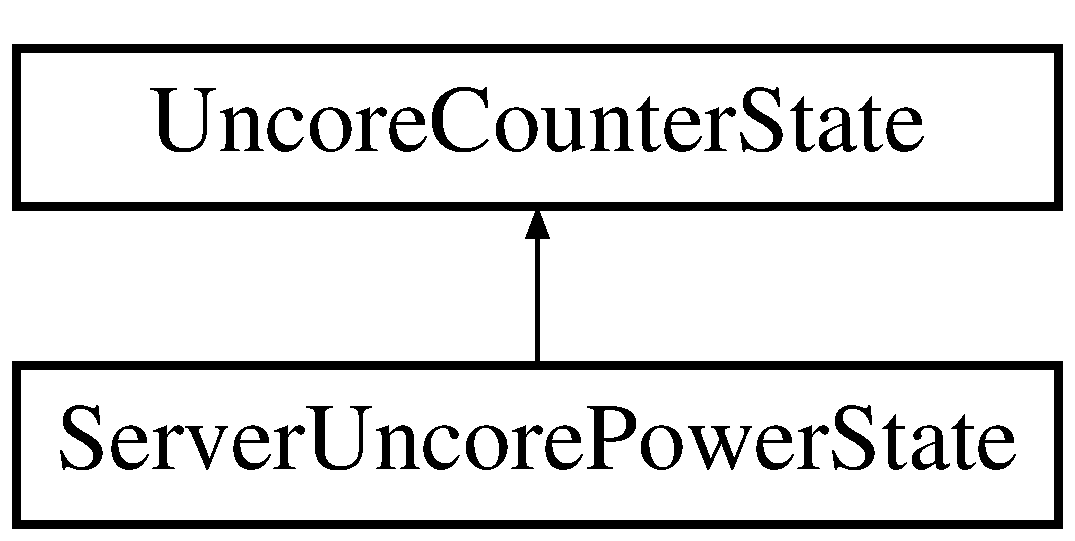
\includegraphics[height=2.000000cm]{classServerUncorePowerState}
\end{center}
\end{figure}
\subsection*{Public Member Functions}
\begin{DoxyCompactItemize}
\item 
int32 {\bf get\+Package\+Thermal\+Headroom} () const \label{classServerUncorePowerState_a2680b28b8d92da4cf74a3a1c59bf7c1d}

\begin{DoxyCompactList}\small\item\em Returns current thermal headroom below Tj\+Max. \end{DoxyCompactList}\end{DoxyCompactItemize}
\subsection*{Friends}
\begin{DoxyCompactItemize}
\item 
class {\bfseries P\+C\+M}\label{classServerUncorePowerState_ab5f56d2e95ba3daf52c17b8a1d356d64}

\item 
{\footnotesize template$<$class Counter\+State\+Type $>$ }\\uint64 {\bf get\+Q\+P\+I\+Clocks} (uint32 port, const Counter\+State\+Type \&before, const Counter\+State\+Type \&after)
\begin{DoxyCompactList}\small\item\em Returns Q\+P\+I L\+L clock ticks. \end{DoxyCompactList}\item 
{\footnotesize template$<$class Counter\+State\+Type $>$ }\\uint64 {\bf get\+Q\+P\+I\+L0p\+Tx\+Cycles} (uint32 port, const Counter\+State\+Type \&before, const Counter\+State\+Type \&after)
\begin{DoxyCompactList}\small\item\em Returns the number of Q\+P\+I cycles in power saving half-\/lane mode. \end{DoxyCompactList}\item 
{\footnotesize template$<$class Counter\+State\+Type $>$ }\\uint64 {\bf get\+Q\+P\+I\+L1\+Cycles} (uint32 port, const Counter\+State\+Type \&before, const Counter\+State\+Type \&after)
\begin{DoxyCompactList}\small\item\em Returns the number of Q\+P\+I cycles in power saving shutdown mode. \end{DoxyCompactList}\item 
{\footnotesize template$<$class Counter\+State\+Type $>$ }\\uint64 {\bf get\+D\+R\+A\+M\+Clocks} (uint32 channel, const Counter\+State\+Type \&before, const Counter\+State\+Type \&after)
\begin{DoxyCompactList}\small\item\em Returns D\+R\+A\+M clock ticks. \end{DoxyCompactList}\item 
{\footnotesize template$<$class Counter\+State\+Type $>$ }\\uint64 {\bf get\+M\+C\+Counter} (uint32 channel, uint32 counter, const Counter\+State\+Type \&before, const Counter\+State\+Type \&after)
\begin{DoxyCompactList}\small\item\em Direct read of memory controller P\+M\+U counter (counter meaning depends on the programming\+: power/performance/etc) \end{DoxyCompactList}\item 
{\footnotesize template$<$class Counter\+State\+Type $>$ }\\uint64 {\bf get\+P\+C\+U\+Counter} (uint32 counter, const Counter\+State\+Type \&before, const Counter\+State\+Type \&after)
\begin{DoxyCompactList}\small\item\em Direct read of power control unit P\+M\+U counter (counter meaning depends on the programming\+: power/performance/etc) \end{DoxyCompactList}\item 
{\footnotesize template$<$class Counter\+State\+Type $>$ }\\uint64 {\bf get\+Consumed\+Energy} (const Counter\+State\+Type \&before, const Counter\+State\+Type \&after)
\begin{DoxyCompactList}\small\item\em Returns energy consumed by processor, exclusing D\+R\+A\+M (measured in internal units) \end{DoxyCompactList}\item 
{\footnotesize template$<$class Counter\+State\+Type $>$ }\\uint64 {\bf get\+D\+R\+A\+M\+Consumed\+Energy} (const Counter\+State\+Type \&before, const Counter\+State\+Type \&after)
\begin{DoxyCompactList}\small\item\em Returns energy consumed by D\+R\+A\+M (measured in internal units) \end{DoxyCompactList}\item 
{\footnotesize template$<$class Counter\+State\+Type $>$ }\\uint64 {\bf get\+Invariant\+T\+S\+C} (const Counter\+State\+Type \&before, const Counter\+State\+Type \&after)
\begin{DoxyCompactList}\small\item\em Computes number of invariant time stamp counter ticks. \end{DoxyCompactList}\end{DoxyCompactItemize}
\subsection*{Additional Inherited Members}


\subsection{Detailed Description}
Server uncore power counter state. 

\subsection{Friends And Related Function Documentation}
\index{Server\+Uncore\+Power\+State@{Server\+Uncore\+Power\+State}!get\+Consumed\+Energy@{get\+Consumed\+Energy}}
\index{get\+Consumed\+Energy@{get\+Consumed\+Energy}!Server\+Uncore\+Power\+State@{Server\+Uncore\+Power\+State}}
\subsubsection[{get\+Consumed\+Energy}]{\setlength{\rightskip}{0pt plus 5cm}template$<$class Counter\+State\+Type $>$ uint64 get\+Consumed\+Energy (
\begin{DoxyParamCaption}
\item[{const Counter\+State\+Type \&}]{before, }
\item[{const Counter\+State\+Type \&}]{after}
\end{DoxyParamCaption}
)\hspace{0.3cm}{\ttfamily [friend]}}\label{classServerUncorePowerState_a054b949f09283093e1923affa4e58ae8}


Returns energy consumed by processor, exclusing D\+R\+A\+M (measured in internal units) 


\begin{DoxyParams}{Parameters}
{\em before} & C\+P\+U counter state before the experiment \\
\hline
{\em after} & C\+P\+U counter state after the experiment \\
\hline
\end{DoxyParams}
\index{Server\+Uncore\+Power\+State@{Server\+Uncore\+Power\+State}!get\+D\+R\+A\+M\+Clocks@{get\+D\+R\+A\+M\+Clocks}}
\index{get\+D\+R\+A\+M\+Clocks@{get\+D\+R\+A\+M\+Clocks}!Server\+Uncore\+Power\+State@{Server\+Uncore\+Power\+State}}
\subsubsection[{get\+D\+R\+A\+M\+Clocks}]{\setlength{\rightskip}{0pt plus 5cm}template$<$class Counter\+State\+Type $>$ uint64 get\+D\+R\+A\+M\+Clocks (
\begin{DoxyParamCaption}
\item[{uint32}]{channel, }
\item[{const Counter\+State\+Type \&}]{before, }
\item[{const Counter\+State\+Type \&}]{after}
\end{DoxyParamCaption}
)\hspace{0.3cm}{\ttfamily [friend]}}\label{classServerUncorePowerState_aeb1baf7feb391c0512dc378a9fd66a17}


Returns D\+R\+A\+M clock ticks. 


\begin{DoxyParams}{Parameters}
{\em channel} & D\+R\+A\+M channel number \\
\hline
{\em before} & C\+P\+U counter state before the experiment \\
\hline
{\em after} & C\+P\+U counter state after the experiment \\
\hline
\end{DoxyParams}
\index{Server\+Uncore\+Power\+State@{Server\+Uncore\+Power\+State}!get\+D\+R\+A\+M\+Consumed\+Energy@{get\+D\+R\+A\+M\+Consumed\+Energy}}
\index{get\+D\+R\+A\+M\+Consumed\+Energy@{get\+D\+R\+A\+M\+Consumed\+Energy}!Server\+Uncore\+Power\+State@{Server\+Uncore\+Power\+State}}
\subsubsection[{get\+D\+R\+A\+M\+Consumed\+Energy}]{\setlength{\rightskip}{0pt plus 5cm}template$<$class Counter\+State\+Type $>$ uint64 get\+D\+R\+A\+M\+Consumed\+Energy (
\begin{DoxyParamCaption}
\item[{const Counter\+State\+Type \&}]{before, }
\item[{const Counter\+State\+Type \&}]{after}
\end{DoxyParamCaption}
)\hspace{0.3cm}{\ttfamily [friend]}}\label{classServerUncorePowerState_a71af0766460ef7dd3d138ec0d0924eda}


Returns energy consumed by D\+R\+A\+M (measured in internal units) 


\begin{DoxyParams}{Parameters}
{\em before} & C\+P\+U counter state before the experiment \\
\hline
{\em after} & C\+P\+U counter state after the experiment \\
\hline
\end{DoxyParams}
\index{Server\+Uncore\+Power\+State@{Server\+Uncore\+Power\+State}!get\+Invariant\+T\+S\+C@{get\+Invariant\+T\+S\+C}}
\index{get\+Invariant\+T\+S\+C@{get\+Invariant\+T\+S\+C}!Server\+Uncore\+Power\+State@{Server\+Uncore\+Power\+State}}
\subsubsection[{get\+Invariant\+T\+S\+C}]{\setlength{\rightskip}{0pt plus 5cm}template$<$class Counter\+State\+Type $>$ uint64 get\+Invariant\+T\+S\+C (
\begin{DoxyParamCaption}
\item[{const Counter\+State\+Type \&}]{before, }
\item[{const Counter\+State\+Type \&}]{after}
\end{DoxyParamCaption}
)\hspace{0.3cm}{\ttfamily [friend]}}\label{classServerUncorePowerState_a45cf07a8d3ce2c48968842554a3854f9}


Computes number of invariant time stamp counter ticks. 

This counter counts irrespectively of C-\/, P-\/ or T-\/states


\begin{DoxyParams}{Parameters}
{\em before} & C\+P\+U counter state before the experiment \\
\hline
{\em after} & C\+P\+U counter state after the experiment \\
\hline
\end{DoxyParams}
\begin{DoxyReturn}{Returns}
number of time stamp counter ticks 
\end{DoxyReturn}
\index{Server\+Uncore\+Power\+State@{Server\+Uncore\+Power\+State}!get\+M\+C\+Counter@{get\+M\+C\+Counter}}
\index{get\+M\+C\+Counter@{get\+M\+C\+Counter}!Server\+Uncore\+Power\+State@{Server\+Uncore\+Power\+State}}
\subsubsection[{get\+M\+C\+Counter}]{\setlength{\rightskip}{0pt plus 5cm}template$<$class Counter\+State\+Type $>$ uint64 get\+M\+C\+Counter (
\begin{DoxyParamCaption}
\item[{uint32}]{channel, }
\item[{uint32}]{counter, }
\item[{const Counter\+State\+Type \&}]{before, }
\item[{const Counter\+State\+Type \&}]{after}
\end{DoxyParamCaption}
)\hspace{0.3cm}{\ttfamily [friend]}}\label{classServerUncorePowerState_aed082cc97dbad35e1633823e582afa0f}


Direct read of memory controller P\+M\+U counter (counter meaning depends on the programming\+: power/performance/etc) 


\begin{DoxyParams}{Parameters}
{\em counter} & counter number \\
\hline
{\em channel} & channel number \\
\hline
{\em before} & C\+P\+U counter state before the experiment \\
\hline
{\em after} & C\+P\+U counter state after the experiment \\
\hline
\end{DoxyParams}
\index{Server\+Uncore\+Power\+State@{Server\+Uncore\+Power\+State}!get\+P\+C\+U\+Counter@{get\+P\+C\+U\+Counter}}
\index{get\+P\+C\+U\+Counter@{get\+P\+C\+U\+Counter}!Server\+Uncore\+Power\+State@{Server\+Uncore\+Power\+State}}
\subsubsection[{get\+P\+C\+U\+Counter}]{\setlength{\rightskip}{0pt plus 5cm}template$<$class Counter\+State\+Type $>$ uint64 get\+P\+C\+U\+Counter (
\begin{DoxyParamCaption}
\item[{uint32}]{counter, }
\item[{const Counter\+State\+Type \&}]{before, }
\item[{const Counter\+State\+Type \&}]{after}
\end{DoxyParamCaption}
)\hspace{0.3cm}{\ttfamily [friend]}}\label{classServerUncorePowerState_a3c424ad42d2439410d6ffc371335573d}


Direct read of power control unit P\+M\+U counter (counter meaning depends on the programming\+: power/performance/etc) 


\begin{DoxyParams}{Parameters}
{\em counter} & counter number \\
\hline
{\em before} & C\+P\+U counter state before the experiment \\
\hline
{\em after} & C\+P\+U counter state after the experiment \\
\hline
\end{DoxyParams}
\index{Server\+Uncore\+Power\+State@{Server\+Uncore\+Power\+State}!get\+Q\+P\+I\+Clocks@{get\+Q\+P\+I\+Clocks}}
\index{get\+Q\+P\+I\+Clocks@{get\+Q\+P\+I\+Clocks}!Server\+Uncore\+Power\+State@{Server\+Uncore\+Power\+State}}
\subsubsection[{get\+Q\+P\+I\+Clocks}]{\setlength{\rightskip}{0pt plus 5cm}template$<$class Counter\+State\+Type $>$ uint64 get\+Q\+P\+I\+Clocks (
\begin{DoxyParamCaption}
\item[{uint32}]{port, }
\item[{const Counter\+State\+Type \&}]{before, }
\item[{const Counter\+State\+Type \&}]{after}
\end{DoxyParamCaption}
)\hspace{0.3cm}{\ttfamily [friend]}}\label{classServerUncorePowerState_af7d9ba0936d7c305d0cc6c2db296a336}


Returns Q\+P\+I L\+L clock ticks. 


\begin{DoxyParams}{Parameters}
{\em port} & Q\+P\+I port number \\
\hline
{\em before} & C\+P\+U counter state before the experiment \\
\hline
{\em after} & C\+P\+U counter state after the experiment \\
\hline
\end{DoxyParams}
\index{Server\+Uncore\+Power\+State@{Server\+Uncore\+Power\+State}!get\+Q\+P\+I\+L0p\+Tx\+Cycles@{get\+Q\+P\+I\+L0p\+Tx\+Cycles}}
\index{get\+Q\+P\+I\+L0p\+Tx\+Cycles@{get\+Q\+P\+I\+L0p\+Tx\+Cycles}!Server\+Uncore\+Power\+State@{Server\+Uncore\+Power\+State}}
\subsubsection[{get\+Q\+P\+I\+L0p\+Tx\+Cycles}]{\setlength{\rightskip}{0pt plus 5cm}template$<$class Counter\+State\+Type $>$ uint64 get\+Q\+P\+I\+L0p\+Tx\+Cycles (
\begin{DoxyParamCaption}
\item[{uint32}]{port, }
\item[{const Counter\+State\+Type \&}]{before, }
\item[{const Counter\+State\+Type \&}]{after}
\end{DoxyParamCaption}
)\hspace{0.3cm}{\ttfamily [friend]}}\label{classServerUncorePowerState_acdac5d9d7a5a6496d90b0681badc26b3}


Returns the number of Q\+P\+I cycles in power saving half-\/lane mode. 


\begin{DoxyParams}{Parameters}
{\em port} & Q\+P\+I port number \\
\hline
{\em before} & C\+P\+U counter state before the experiment \\
\hline
{\em after} & C\+P\+U counter state after the experiment \\
\hline
\end{DoxyParams}
\index{Server\+Uncore\+Power\+State@{Server\+Uncore\+Power\+State}!get\+Q\+P\+I\+L1\+Cycles@{get\+Q\+P\+I\+L1\+Cycles}}
\index{get\+Q\+P\+I\+L1\+Cycles@{get\+Q\+P\+I\+L1\+Cycles}!Server\+Uncore\+Power\+State@{Server\+Uncore\+Power\+State}}
\subsubsection[{get\+Q\+P\+I\+L1\+Cycles}]{\setlength{\rightskip}{0pt plus 5cm}template$<$class Counter\+State\+Type $>$ uint64 get\+Q\+P\+I\+L1\+Cycles (
\begin{DoxyParamCaption}
\item[{uint32}]{port, }
\item[{const Counter\+State\+Type \&}]{before, }
\item[{const Counter\+State\+Type \&}]{after}
\end{DoxyParamCaption}
)\hspace{0.3cm}{\ttfamily [friend]}}\label{classServerUncorePowerState_a580ae4e465d0f8dd93935ad7af28c095}


Returns the number of Q\+P\+I cycles in power saving shutdown mode. 


\begin{DoxyParams}{Parameters}
{\em port} & Q\+P\+I port number \\
\hline
{\em before} & C\+P\+U counter state before the experiment \\
\hline
{\em after} & C\+P\+U counter state after the experiment \\
\hline
\end{DoxyParams}


The documentation for this class was generated from the following file\+:\begin{DoxyCompactItemize}
\item 
{\bf cpucounters.\+h}\end{DoxyCompactItemize}

\section{Socket\+Counter\+State Class Reference}
\label{classSocketCounterState}\index{Socket\+Counter\+State@{Socket\+Counter\+State}}


Socket-\/wide counter state.  




{\ttfamily \#include $<$cpucounters.\+h$>$}

Inheritance diagram for Socket\+Counter\+State\+:\begin{figure}[H]
\begin{center}
\leavevmode
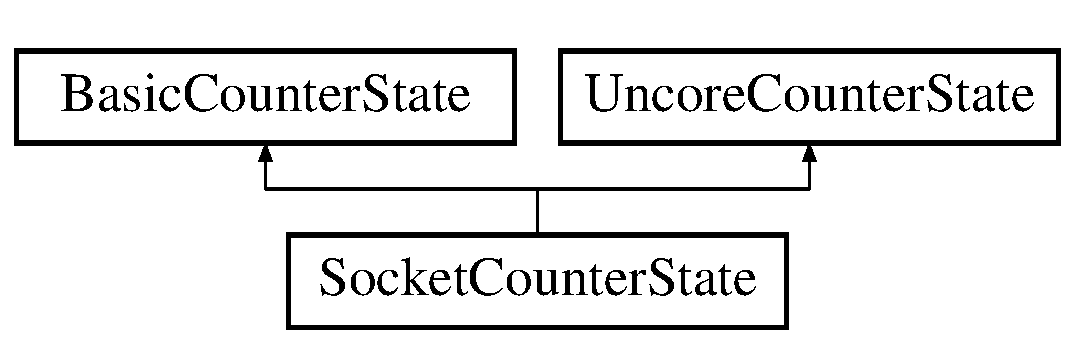
\includegraphics[height=2.000000cm]{classSocketCounterState}
\end{center}
\end{figure}
\subsection*{Public Member Functions}
\begin{DoxyCompactItemize}
\item 
void {\bfseries accumulate\+Core\+State} (const {\bf Core\+Counter\+State} \&o)\label{classSocketCounterState_aa23362a4685d2abad8c2c7264bb47eab}

\end{DoxyCompactItemize}
\subsection*{Protected Member Functions}
\begin{DoxyCompactItemize}
\item 
void {\bfseries read\+And\+Aggregate} ({\bf Safe\+Msr\+Handle} $\ast$handle)\label{classSocketCounterState_a6525d0eda2a11ad906b16cb05ee5c0e5}

\end{DoxyCompactItemize}
\subsection*{Friends}
\begin{DoxyCompactItemize}
\item 
class {\bfseries P\+C\+M}\label{classSocketCounterState_ab5f56d2e95ba3daf52c17b8a1d356d64}

\end{DoxyCompactItemize}
\subsection*{Additional Inherited Members}


\subsection{Detailed Description}
Socket-\/wide counter state. 

The documentation for this class was generated from the following file\+:\begin{DoxyCompactItemize}
\item 
{\bf cpucounters.\+h}\end{DoxyCompactItemize}

\section{System\+Counter\+State Class Reference}
\label{classSystemCounterState}\index{System\+Counter\+State@{System\+Counter\+State}}


System-\/wide counter state.  




{\ttfamily \#include $<$cpucounters.\+h$>$}

Inheritance diagram for System\+Counter\+State\+:\begin{figure}[H]
\begin{center}
\leavevmode
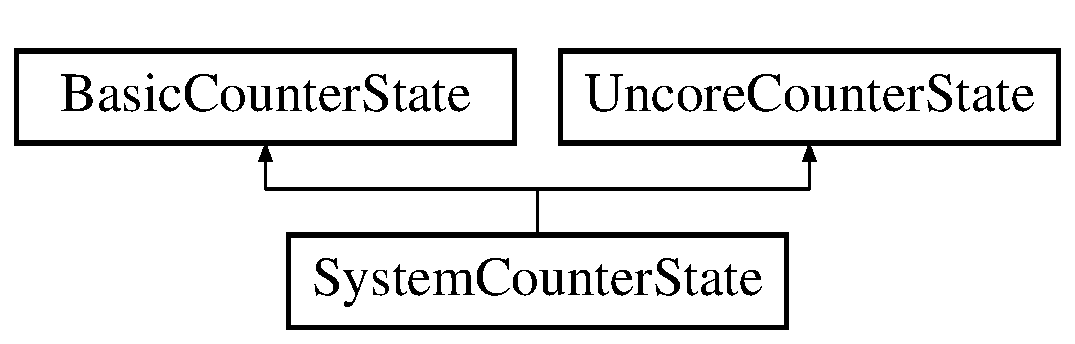
\includegraphics[height=2.000000cm]{classSystemCounterState}
\end{center}
\end{figure}
\subsection*{Public Member Functions}
\begin{DoxyCompactItemize}
\item 
void {\bfseries accumulate\+Socket\+State} (const {\bf Socket\+Counter\+State} \&o)\label{classSystemCounterState_af8fb0cdf2c4d03ec03b1ef2e4c27aac4}

\end{DoxyCompactItemize}
\subsection*{Protected Member Functions}
\begin{DoxyCompactItemize}
\item 
void {\bfseries read\+And\+Aggregate} ({\bf Safe\+Msr\+Handle} $\ast$handle)\label{classSystemCounterState_a8fe045dbb23a309ecd8ec75cf5563c60}

\end{DoxyCompactItemize}
\subsection*{Friends}
\begin{DoxyCompactItemize}
\item 
class {\bfseries P\+C\+M}\label{classSystemCounterState_ab5f56d2e95ba3daf52c17b8a1d356d64}

\item 
uint64 {\bf get\+Incoming\+Q\+P\+I\+Link\+Bytes} (uint32 socket\+Nr, uint32 link\+Nr, const {\bf System\+Counter\+State} \&before, const {\bf System\+Counter\+State} \&after)
\begin{DoxyCompactList}\small\item\em Get estimation of Q\+P\+I data traffic per incoming Q\+P\+I link. \end{DoxyCompactList}\item 
uint64 {\bf get\+Incoming\+Q\+P\+I\+Link\+Bytes} (uint32 socket\+Nr, uint32 link\+Nr, const {\bf System\+Counter\+State} \&now)
\begin{DoxyCompactList}\small\item\em Return current value of the counter of Q\+P\+I data traffic per incoming Q\+P\+I link. \end{DoxyCompactList}\item 
double {\bf get\+Outgoing\+Q\+P\+I\+Link\+Utilization} (uint32 socket\+Nr, uint32 link\+Nr, const {\bf System\+Counter\+State} \&before, const {\bf System\+Counter\+State} \&after)
\begin{DoxyCompactList}\small\item\em Get utilization of outgoing Q\+P\+I link (0..1) \end{DoxyCompactList}\item 
uint64 {\bf get\+Outgoing\+Q\+P\+I\+Link\+Bytes} (uint32 socket\+Nr, uint32 link\+Nr, const {\bf System\+Counter\+State} \&before, const {\bf System\+Counter\+State} \&after)
\begin{DoxyCompactList}\small\item\em Get estimation of Q\+P\+I (data+nondata) traffic per outgoing Q\+P\+I link. \end{DoxyCompactList}\item 
uint64 {\bfseries get\+Outgoing\+Q\+P\+I\+Link\+Bytes} (uint32 socket\+Nr, uint32 link\+Nr, const {\bf System\+Counter\+State} \&now)\label{classSystemCounterState_a336f198b4a81e0d34bb581e8bd8be0e0}

\end{DoxyCompactItemize}
\subsection*{Additional Inherited Members}


\subsection{Detailed Description}
System-\/wide counter state. 

\subsection{Friends And Related Function Documentation}
\index{System\+Counter\+State@{System\+Counter\+State}!get\+Incoming\+Q\+P\+I\+Link\+Bytes@{get\+Incoming\+Q\+P\+I\+Link\+Bytes}}
\index{get\+Incoming\+Q\+P\+I\+Link\+Bytes@{get\+Incoming\+Q\+P\+I\+Link\+Bytes}!System\+Counter\+State@{System\+Counter\+State}}
\subsubsection[{get\+Incoming\+Q\+P\+I\+Link\+Bytes}]{\setlength{\rightskip}{0pt plus 5cm}uint64 get\+Incoming\+Q\+P\+I\+Link\+Bytes (
\begin{DoxyParamCaption}
\item[{uint32}]{socket\+Nr, }
\item[{uint32}]{link\+Nr, }
\item[{const {\bf System\+Counter\+State} \&}]{before, }
\item[{const {\bf System\+Counter\+State} \&}]{after}
\end{DoxyParamCaption}
)\hspace{0.3cm}{\ttfamily [friend]}}\label{classSystemCounterState_aca1b1d8ba1679c4a0c394c2647428fd3}


Get estimation of Q\+P\+I data traffic per incoming Q\+P\+I link. 

Returns an estimation of number of data bytes transferred to a socket over Intel(r) Quick Path Interconnect


\begin{DoxyParams}{Parameters}
{\em socket\+Nr} & socket identifier \\
\hline
{\em link\+Nr} & link\+Nr \\
\hline
{\em before} & System C\+P\+U counter state before the experiment \\
\hline
{\em after} & System C\+P\+U counter state after the experiment \\
\hline
\end{DoxyParams}
\begin{DoxyReturn}{Returns}
Number of bytes 
\end{DoxyReturn}
\index{System\+Counter\+State@{System\+Counter\+State}!get\+Incoming\+Q\+P\+I\+Link\+Bytes@{get\+Incoming\+Q\+P\+I\+Link\+Bytes}}
\index{get\+Incoming\+Q\+P\+I\+Link\+Bytes@{get\+Incoming\+Q\+P\+I\+Link\+Bytes}!System\+Counter\+State@{System\+Counter\+State}}
\subsubsection[{get\+Incoming\+Q\+P\+I\+Link\+Bytes}]{\setlength{\rightskip}{0pt plus 5cm}uint64 get\+Incoming\+Q\+P\+I\+Link\+Bytes (
\begin{DoxyParamCaption}
\item[{uint32}]{socket\+Nr, }
\item[{uint32}]{link\+Nr, }
\item[{const {\bf System\+Counter\+State} \&}]{now}
\end{DoxyParamCaption}
)\hspace{0.3cm}{\ttfamily [friend]}}\label{classSystemCounterState_a42d6a119a26ea41c40d5585356d832ca}


Return current value of the counter of Q\+P\+I data traffic per incoming Q\+P\+I link. 

Returns the number of incoming data bytes to a socket over Intel(r) Quick Path Interconnect


\begin{DoxyParams}{Parameters}
{\em socket\+Nr} & socket identifier \\
\hline
{\em link\+Nr} & link\+Nr \\
\hline
{\em now} & Current System C\+P\+U counter state \\
\hline
\end{DoxyParams}
\begin{DoxyReturn}{Returns}
Number of bytes 
\end{DoxyReturn}
\index{System\+Counter\+State@{System\+Counter\+State}!get\+Outgoing\+Q\+P\+I\+Link\+Bytes@{get\+Outgoing\+Q\+P\+I\+Link\+Bytes}}
\index{get\+Outgoing\+Q\+P\+I\+Link\+Bytes@{get\+Outgoing\+Q\+P\+I\+Link\+Bytes}!System\+Counter\+State@{System\+Counter\+State}}
\subsubsection[{get\+Outgoing\+Q\+P\+I\+Link\+Bytes}]{\setlength{\rightskip}{0pt plus 5cm}uint64 get\+Outgoing\+Q\+P\+I\+Link\+Bytes (
\begin{DoxyParamCaption}
\item[{uint32}]{socket\+Nr, }
\item[{uint32}]{link\+Nr, }
\item[{const {\bf System\+Counter\+State} \&}]{before, }
\item[{const {\bf System\+Counter\+State} \&}]{after}
\end{DoxyParamCaption}
)\hspace{0.3cm}{\ttfamily [friend]}}\label{classSystemCounterState_a6bdb34d102d7353421bd878da7b9ef23}


Get estimation of Q\+P\+I (data+nondata) traffic per outgoing Q\+P\+I link. 

Returns an estimation of number of data bytes transferred from a socket over Intel(r) Quick Path Interconnect


\begin{DoxyParams}{Parameters}
{\em socket\+Nr} & socket identifier \\
\hline
{\em link\+Nr} & link\+Nr \\
\hline
{\em before} & System C\+P\+U counter state before the experiment \\
\hline
{\em after} & System C\+P\+U counter state after the experiment \\
\hline
\end{DoxyParams}
\begin{DoxyReturn}{Returns}
Number of bytes 
\end{DoxyReturn}
\index{System\+Counter\+State@{System\+Counter\+State}!get\+Outgoing\+Q\+P\+I\+Link\+Utilization@{get\+Outgoing\+Q\+P\+I\+Link\+Utilization}}
\index{get\+Outgoing\+Q\+P\+I\+Link\+Utilization@{get\+Outgoing\+Q\+P\+I\+Link\+Utilization}!System\+Counter\+State@{System\+Counter\+State}}
\subsubsection[{get\+Outgoing\+Q\+P\+I\+Link\+Utilization}]{\setlength{\rightskip}{0pt plus 5cm}double get\+Outgoing\+Q\+P\+I\+Link\+Utilization (
\begin{DoxyParamCaption}
\item[{uint32}]{socket\+Nr, }
\item[{uint32}]{link\+Nr, }
\item[{const {\bf System\+Counter\+State} \&}]{before, }
\item[{const {\bf System\+Counter\+State} \&}]{after}
\end{DoxyParamCaption}
)\hspace{0.3cm}{\ttfamily [friend]}}\label{classSystemCounterState_ac7b1863133a9a711117fcb8b68d2d773}


Get utilization of outgoing Q\+P\+I link (0..1) 

Returns an estimation of utilization of Q\+P\+I link by (data+nondata) traffic transferred from a socket over Intel(r) Quick Path Interconnect


\begin{DoxyParams}{Parameters}
{\em socket\+Nr} & socket identifier \\
\hline
{\em link\+Nr} & link\+Nr \\
\hline
{\em before} & System C\+P\+U counter state before the experiment \\
\hline
{\em after} & System C\+P\+U counter state after the experiment \\
\hline
\end{DoxyParams}
\begin{DoxyReturn}{Returns}
utilization (0..1) 
\end{DoxyReturn}


The documentation for this class was generated from the following file\+:\begin{DoxyCompactItemize}
\item 
{\bf cpucounters.\+h}\end{DoxyCompactItemize}

\section{T Struct Reference}
\label{structT}\index{T@{T}}
\subsection*{Public Member Functions}
\begin{DoxyCompactItemize}
\item 
{\bfseries T} (int a)\label{structT_a8f5edc9a39e3241d33ae54a5029b0043}

\item 
bool {\bfseries operator==} (const {\bf T} \&k) const \label{structT_aac67a90aee0b9034ea177ce4676052bf}

\item 
{\bfseries T} (int a)\label{structT_a8f5edc9a39e3241d33ae54a5029b0043}

\item 
bool {\bfseries operator==} (const {\bf T} \&k) const \label{structT_aac67a90aee0b9034ea177ce4676052bf}

\item 
{\bfseries T} (int a)\label{structT_a8f5edc9a39e3241d33ae54a5029b0043}

\item 
bool {\bfseries operator==} (const {\bf T} \&k) const \label{structT_aac67a90aee0b9034ea177ce4676052bf}

\end{DoxyCompactItemize}
\subsection*{Public Attributes}
\begin{DoxyCompactItemize}
\item 
int {\bfseries key} [1]\label{structT_a910785bad87bed60eccfe8fec17e55ec}

\item 
int {\bfseries data} [3]\label{structT_a07547b3bcc7ade309011aaa5a56ec814}

\end{DoxyCompactItemize}


The documentation for this struct was generated from the following files\+:\begin{DoxyCompactItemize}
\item 
memoptest.\+cpp\item 
readmem.\+cpp\item 
{\bf realtime.\+cpp}\end{DoxyCompactItemize}

\section{Temporal\+Thread\+Affinity Class Reference}
\label{classTemporalThreadAffinity}\index{Temporal\+Thread\+Affinity@{Temporal\+Thread\+Affinity}}
\subsection*{Public Member Functions}
\begin{DoxyCompactItemize}
\item 
{\bfseries Temporal\+Thread\+Affinity} (uint32)\label{classTemporalThreadAffinity_adc237efcc45938f0c188e705b2ed226e}

\end{DoxyCompactItemize}


The documentation for this class was generated from the following file\+:\begin{DoxyCompactItemize}
\item 
{\bf cpucounters.\+cpp}\end{DoxyCompactItemize}

\section{Topology\+Entry Struct Reference}
\label{structTopologyEntry}\index{Topology\+Entry@{Topology\+Entry}}
\subsection*{Public Attributes}
\begin{DoxyCompactItemize}
\item 
int32 {\bfseries os\+\_\+id}\label{structTopologyEntry_aa960a8bbdd754740d781072ae1266eed}

\item 
int32 {\bfseries socket}\label{structTopologyEntry_a9b217468c64b3072b48ad5466742827e}

\item 
int32 {\bfseries core\+\_\+id}\label{structTopologyEntry_aee7bef9e2b54f9617a697a43068a5c27}

\end{DoxyCompactItemize}


The documentation for this struct was generated from the following file\+:\begin{DoxyCompactItemize}
\item 
{\bf cpucounters.\+h}\end{DoxyCompactItemize}

\section{T\+S\+X\+Event Struct Reference}
\label{structTSXEvent}\index{T\+S\+X\+Event@{T\+S\+X\+Event}}
\subsection*{Public Attributes}
\begin{DoxyCompactItemize}
\item 
const char $\ast$ {\bfseries name}\label{structTSXEvent_a592441448f28d73655c864f5dbb77538}

\item 
unsigned char {\bfseries event}\label{structTSXEvent_a45969e694e699c485379594701bd7e35}

\item 
unsigned char {\bfseries umask}\label{structTSXEvent_a2f1b2f588a4641abde0dd5bd7870a537}

\item 
const char $\ast$ {\bfseries description}\label{structTSXEvent_aae0d6de90f1596c51b6c0345356a1076}

\end{DoxyCompactItemize}


The documentation for this struct was generated from the following file\+:\begin{DoxyCompactItemize}
\item 
{\bf pcm-\/tsx.\+cpp}\end{DoxyCompactItemize}

\section{Uncore\+Counter\+State Class Reference}
\label{classUncoreCounterState}\index{Uncore\+Counter\+State@{Uncore\+Counter\+State}}


Basic uncore counter state.  




{\ttfamily \#include $<$cpucounters.\+h$>$}

Inheritance diagram for Uncore\+Counter\+State\+:\begin{figure}[H]
\begin{center}
\leavevmode
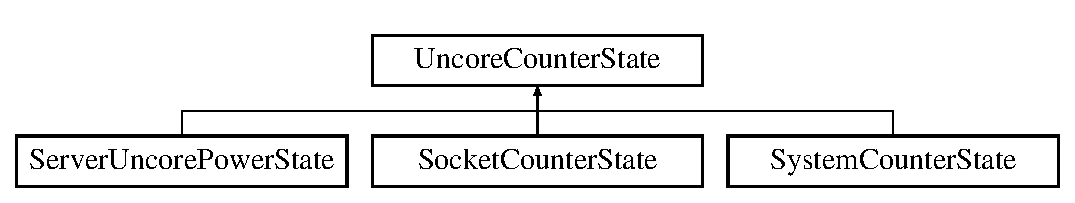
\includegraphics[height=2.000000cm]{classUncoreCounterState}
\end{center}
\end{figure}
\subsection*{Public Member Functions}
\begin{DoxyCompactItemize}
\item 
{\bf Uncore\+Counter\+State} \& {\bfseries operator+=} (const {\bf Uncore\+Counter\+State} \&o)\label{classUncoreCounterState_a96eb270d92f202a85ed11ded8cf60f71}

\end{DoxyCompactItemize}
\subsection*{Protected Member Functions}
\begin{DoxyCompactItemize}
\item 
void {\bfseries read\+And\+Aggregate} ({\bf Safe\+Msr\+Handle} $\ast$)\label{classUncoreCounterState_a7c3a2c7c2aab86c21a7a216fac3cf092}

\end{DoxyCompactItemize}
\subsection*{Protected Attributes}
\begin{DoxyCompactItemize}
\item 
uint64 {\bfseries Unc\+M\+C\+Full\+Writes}\label{classUncoreCounterState_a3e59bb4c79f6040b17b104194a5e29fb}

\item 
uint64 {\bfseries Unc\+M\+C\+Normal\+Reads}\label{classUncoreCounterState_a5a07c23a907365682137c5d8c1cf79ad}

\item 
uint64 {\bfseries Unc\+M\+C\+I\+O\+Requests}\label{classUncoreCounterState_a4c3d0db74283d9420d9089e2c2553561}

\item 
uint64 {\bfseries Package\+Energy\+Status}\label{classUncoreCounterState_a74bdee47e68bbc55c2ee023fc3bfe76d}

\item 
uint64 {\bfseries D\+R\+A\+M\+Energy\+Status}\label{classUncoreCounterState_a03c78bbb9fb36c84c075b8d72fc5eed9}

\item 
uint64 {\bfseries C\+State\+Residency} [P\+C\+M\+::\+M\+A\+X\+\_\+\+C\+\_\+\+S\+T\+A\+T\+E+1]\label{classUncoreCounterState_a5819f82036b4386ca638d0755cdc7388}

\end{DoxyCompactItemize}
\subsection*{Friends}
\begin{DoxyCompactItemize}
\item 
class {\bfseries P\+C\+M}\label{classUncoreCounterState_ab5f56d2e95ba3daf52c17b8a1d356d64}

\item 
{\footnotesize template$<$class Counter\+State\+Type $>$ }\\uint64 {\bf get\+Bytes\+Read\+From\+M\+C} (const Counter\+State\+Type \&before, const Counter\+State\+Type \&after)
\begin{DoxyCompactList}\small\item\em Computes number of bytes read from D\+R\+A\+M memory controllers. \end{DoxyCompactList}\item 
{\footnotesize template$<$class Counter\+State\+Type $>$ }\\uint64 {\bf get\+Bytes\+Written\+To\+M\+C} (const Counter\+State\+Type \&before, const Counter\+State\+Type \&after)
\begin{DoxyCompactList}\small\item\em Computes number of bytes written to D\+R\+A\+M memory controllers. \end{DoxyCompactList}\item 
{\footnotesize template$<$class Counter\+State\+Type $>$ }\\uint64 {\bf get\+I\+O\+Request\+Bytes\+From\+M\+C} (const Counter\+State\+Type \&before, const Counter\+State\+Type \&after)
\begin{DoxyCompactList}\small\item\em Computes number of bytes of read/write requests from all I\+O sources. \end{DoxyCompactList}\item 
{\footnotesize template$<$class Counter\+State\+Type $>$ }\\uint64 {\bf get\+Consumed\+Energy} (const Counter\+State\+Type \&before, const Counter\+State\+Type \&after)
\begin{DoxyCompactList}\small\item\em Returns energy consumed by processor, exclusing D\+R\+A\+M (measured in internal units) \end{DoxyCompactList}\item 
{\footnotesize template$<$class Counter\+State\+Type $>$ }\\uint64 {\bf get\+D\+R\+A\+M\+Consumed\+Energy} (const Counter\+State\+Type \&before, const Counter\+State\+Type \&after)
\begin{DoxyCompactList}\small\item\em Returns energy consumed by D\+R\+A\+M (measured in internal units) \end{DoxyCompactList}\item 
{\footnotesize template$<$class Counter\+State\+Type $>$ }\\double {\bf get\+Package\+C\+State\+Residency} (int state, const Counter\+State\+Type \&before, const Counter\+State\+Type \&after)
\begin{DoxyCompactList}\small\item\em Computes residency in the package C-\/state. \end{DoxyCompactList}\end{DoxyCompactItemize}


\subsection{Detailed Description}
Basic uncore counter state. 

Intended only for derivation, but not for the direct use 

\subsection{Friends And Related Function Documentation}
\index{Uncore\+Counter\+State@{Uncore\+Counter\+State}!get\+Bytes\+Read\+From\+M\+C@{get\+Bytes\+Read\+From\+M\+C}}
\index{get\+Bytes\+Read\+From\+M\+C@{get\+Bytes\+Read\+From\+M\+C}!Uncore\+Counter\+State@{Uncore\+Counter\+State}}
\subsubsection[{get\+Bytes\+Read\+From\+M\+C}]{\setlength{\rightskip}{0pt plus 5cm}template$<$class Counter\+State\+Type $>$ uint64 get\+Bytes\+Read\+From\+M\+C (
\begin{DoxyParamCaption}
\item[{const Counter\+State\+Type \&}]{before, }
\item[{const Counter\+State\+Type \&}]{after}
\end{DoxyParamCaption}
)\hspace{0.3cm}{\ttfamily [friend]}}\label{classUncoreCounterState_a0f28a32a3edeaecd916ba097aee99d7f}


Computes number of bytes read from D\+R\+A\+M memory controllers. 


\begin{DoxyParams}{Parameters}
{\em before} & C\+P\+U counter state before the experiment \\
\hline
{\em after} & C\+P\+U counter state after the experiment \\
\hline
\end{DoxyParams}
\begin{DoxyReturn}{Returns}
Number of bytes 
\end{DoxyReturn}
\index{Uncore\+Counter\+State@{Uncore\+Counter\+State}!get\+Bytes\+Written\+To\+M\+C@{get\+Bytes\+Written\+To\+M\+C}}
\index{get\+Bytes\+Written\+To\+M\+C@{get\+Bytes\+Written\+To\+M\+C}!Uncore\+Counter\+State@{Uncore\+Counter\+State}}
\subsubsection[{get\+Bytes\+Written\+To\+M\+C}]{\setlength{\rightskip}{0pt plus 5cm}template$<$class Counter\+State\+Type $>$ uint64 get\+Bytes\+Written\+To\+M\+C (
\begin{DoxyParamCaption}
\item[{const Counter\+State\+Type \&}]{before, }
\item[{const Counter\+State\+Type \&}]{after}
\end{DoxyParamCaption}
)\hspace{0.3cm}{\ttfamily [friend]}}\label{classUncoreCounterState_a24fce7df2ee7140db18ecfcd74fe63d1}


Computes number of bytes written to D\+R\+A\+M memory controllers. 


\begin{DoxyParams}{Parameters}
{\em before} & C\+P\+U counter state before the experiment \\
\hline
{\em after} & C\+P\+U counter state after the experiment \\
\hline
\end{DoxyParams}
\begin{DoxyReturn}{Returns}
Number of bytes 
\end{DoxyReturn}
\index{Uncore\+Counter\+State@{Uncore\+Counter\+State}!get\+Consumed\+Energy@{get\+Consumed\+Energy}}
\index{get\+Consumed\+Energy@{get\+Consumed\+Energy}!Uncore\+Counter\+State@{Uncore\+Counter\+State}}
\subsubsection[{get\+Consumed\+Energy}]{\setlength{\rightskip}{0pt plus 5cm}template$<$class Counter\+State\+Type $>$ uint64 get\+Consumed\+Energy (
\begin{DoxyParamCaption}
\item[{const Counter\+State\+Type \&}]{before, }
\item[{const Counter\+State\+Type \&}]{after}
\end{DoxyParamCaption}
)\hspace{0.3cm}{\ttfamily [friend]}}\label{classUncoreCounterState_a054b949f09283093e1923affa4e58ae8}


Returns energy consumed by processor, exclusing D\+R\+A\+M (measured in internal units) 


\begin{DoxyParams}{Parameters}
{\em before} & C\+P\+U counter state before the experiment \\
\hline
{\em after} & C\+P\+U counter state after the experiment \\
\hline
\end{DoxyParams}
\index{Uncore\+Counter\+State@{Uncore\+Counter\+State}!get\+D\+R\+A\+M\+Consumed\+Energy@{get\+D\+R\+A\+M\+Consumed\+Energy}}
\index{get\+D\+R\+A\+M\+Consumed\+Energy@{get\+D\+R\+A\+M\+Consumed\+Energy}!Uncore\+Counter\+State@{Uncore\+Counter\+State}}
\subsubsection[{get\+D\+R\+A\+M\+Consumed\+Energy}]{\setlength{\rightskip}{0pt plus 5cm}template$<$class Counter\+State\+Type $>$ uint64 get\+D\+R\+A\+M\+Consumed\+Energy (
\begin{DoxyParamCaption}
\item[{const Counter\+State\+Type \&}]{before, }
\item[{const Counter\+State\+Type \&}]{after}
\end{DoxyParamCaption}
)\hspace{0.3cm}{\ttfamily [friend]}}\label{classUncoreCounterState_a71af0766460ef7dd3d138ec0d0924eda}


Returns energy consumed by D\+R\+A\+M (measured in internal units) 


\begin{DoxyParams}{Parameters}
{\em before} & C\+P\+U counter state before the experiment \\
\hline
{\em after} & C\+P\+U counter state after the experiment \\
\hline
\end{DoxyParams}
\index{Uncore\+Counter\+State@{Uncore\+Counter\+State}!get\+I\+O\+Request\+Bytes\+From\+M\+C@{get\+I\+O\+Request\+Bytes\+From\+M\+C}}
\index{get\+I\+O\+Request\+Bytes\+From\+M\+C@{get\+I\+O\+Request\+Bytes\+From\+M\+C}!Uncore\+Counter\+State@{Uncore\+Counter\+State}}
\subsubsection[{get\+I\+O\+Request\+Bytes\+From\+M\+C}]{\setlength{\rightskip}{0pt plus 5cm}template$<$class Counter\+State\+Type $>$ uint64 get\+I\+O\+Request\+Bytes\+From\+M\+C (
\begin{DoxyParamCaption}
\item[{const Counter\+State\+Type \&}]{before, }
\item[{const Counter\+State\+Type \&}]{after}
\end{DoxyParamCaption}
)\hspace{0.3cm}{\ttfamily [friend]}}\label{classUncoreCounterState_a7e5434dba3a810501f289329e52b889d}


Computes number of bytes of read/write requests from all I\+O sources. 


\begin{DoxyParams}{Parameters}
{\em before} & C\+P\+U counter state before the experiment \\
\hline
{\em after} & C\+P\+U counter state after the experiment \\
\hline
\end{DoxyParams}
\begin{DoxyReturn}{Returns}
Number of bytes 
\end{DoxyReturn}
\index{Uncore\+Counter\+State@{Uncore\+Counter\+State}!get\+Package\+C\+State\+Residency@{get\+Package\+C\+State\+Residency}}
\index{get\+Package\+C\+State\+Residency@{get\+Package\+C\+State\+Residency}!Uncore\+Counter\+State@{Uncore\+Counter\+State}}
\subsubsection[{get\+Package\+C\+State\+Residency}]{\setlength{\rightskip}{0pt plus 5cm}template$<$class Counter\+State\+Type $>$ double get\+Package\+C\+State\+Residency (
\begin{DoxyParamCaption}
\item[{int}]{state, }
\item[{const Counter\+State\+Type \&}]{before, }
\item[{const Counter\+State\+Type \&}]{after}
\end{DoxyParamCaption}
)\hspace{0.3cm}{\ttfamily [friend]}}\label{classUncoreCounterState_a5e34f7b0326dda86b54fcb7bb84a0b38}


Computes residency in the package C-\/state. 


\begin{DoxyParams}{Parameters}
{\em state} & C-\/state \\
\hline
{\em before} & C\+P\+U counter state before the experiment \\
\hline
{\em after} & C\+P\+U counter state after the experiment \\
\hline
\end{DoxyParams}
\begin{DoxyReturn}{Returns}
residence ratio (0..1)\+: 0 -\/ 0\%, 1.\+0 -\/ 100\% 
\end{DoxyReturn}


The documentation for this class was generated from the following files\+:\begin{DoxyCompactItemize}
\item 
{\bf cpucounters.\+h}\item 
{\bf cpucounters.\+cpp}\end{DoxyCompactItemize}

\section{Uncore\+Event\+Select\+Register Struct Reference}
\label{structUncoreEventSelectRegister}\index{Uncore\+Event\+Select\+Register@{Uncore\+Event\+Select\+Register}}
\subsection*{Public Attributes}
\begin{DoxyCompactItemize}
\item 
\begin{tabbing}
xx\=xx\=xx\=xx\=xx\=xx\=xx\=xx\=xx\=\kill
union \{\\
\>struct \{\\
\>\>uint64 {\bfseries event\_select}: 8\\
\>\>uint64 {\bfseries umask}: 8\\
\>\>uint64 {\bfseries reserved1}: 1\\
\>\>uint64 {\bfseries occ\_ctr\_rst}: 1\\
\>\>uint64 {\bfseries edge}: 1\\
\>\>uint64 {\bfseries reserved2}: 1\\
\>\>uint64 {\bfseries enable\_pmi}: 1\\
\>\>uint64 {\bfseries reserved3}: 1\\
\>\>uint64 {\bfseries enable}: 1\\
\>\>uint64 {\bfseries invert}: 1\\
\>\>uint64 {\bfseries cmask}: 8\\
\>\>uint64 {\bfseries reservedx}: 32\\
\>\} {\bfseries fields}\\
\>uint64 {\bfseries value}\\
\}; \label{structUncoreEventSelectRegister_a4d0fa3c570e3a77385919505792bacd8}
\\

\end{tabbing}\end{DoxyCompactItemize}


The documentation for this struct was generated from the following file\+:\begin{DoxyCompactItemize}
\item 
{\bf types.\+h}\end{DoxyCompactItemize}

\chapter{File Documentation}
\section{client\+\_\+bw.\+h File Reference}
\label{client__bw_8h}\index{client\+\_\+bw.\+h@{client\+\_\+bw.\+h}}


Interface to access client bandwidth counters.  


{\ttfamily \#include \char`\"{}types.\+h\char`\"{}}\\*
{\ttfamily \#include $<$unistd.\+h$>$}\\*
\subsection*{Classes}
\begin{DoxyCompactItemize}
\item 
class {\bf Client\+B\+W}
\end{DoxyCompactItemize}
\subsection*{Macros}
\begin{DoxyCompactItemize}
\item 
\#define {\bfseries P\+C\+M\+\_\+\+C\+L\+I\+E\+N\+T\+\_\+\+I\+M\+C\+\_\+\+B\+A\+R\+\_\+\+O\+F\+F\+S\+E\+T}~(0x0048)\label{client__bw_8h_aa16cd48b0adede371be77dbc0be2fd9b}

\item 
\#define {\bfseries P\+C\+M\+\_\+\+C\+L\+I\+E\+N\+T\+\_\+\+I\+M\+C\+\_\+\+D\+R\+A\+M\+\_\+\+I\+O\+\_\+\+R\+E\+Q\+E\+S\+T\+S}~(0x5048)\label{client__bw_8h_a2afb60758e870c73eec7e100b6040b47}

\item 
\#define {\bfseries P\+C\+M\+\_\+\+C\+L\+I\+E\+N\+T\+\_\+\+I\+M\+C\+\_\+\+D\+R\+A\+M\+\_\+\+D\+A\+T\+A\+\_\+\+R\+E\+A\+D\+S}~(0x5050)\label{client__bw_8h_a125dc536cbcf631a395c40a183645e89}

\item 
\#define {\bfseries P\+C\+M\+\_\+\+C\+L\+I\+E\+N\+T\+\_\+\+I\+M\+C\+\_\+\+D\+R\+A\+M\+\_\+\+D\+A\+T\+A\+\_\+\+W\+R\+I\+T\+E\+S}~(0x5054)\label{client__bw_8h_aca3e4d8c51b41ea7c8465d3f89659796}

\item 
\#define {\bfseries P\+C\+M\+\_\+\+C\+L\+I\+E\+N\+T\+\_\+\+I\+M\+C\+\_\+\+M\+M\+A\+P\+\_\+\+S\+I\+Z\+E}~(0x6000)\label{client__bw_8h_aa0e78fbc5472bbfb796c575dd9c33dba}

\end{DoxyCompactItemize}


\subsection{Detailed Description}
Interface to access client bandwidth counters. 


\section{cpuasynchcounter.\+h File Reference}
\label{cpuasynchcounter_8h}\index{cpuasynchcounter.\+h@{cpuasynchcounter.\+h}}


Implementation of a P\+O\+S\+I\+X thread that periodically saves the current state of counters and exposes them to other threads.  


{\ttfamily \#include $<$pthread.\+h$>$}\\*
{\ttfamily \#include $<$stdlib.\+h$>$}\\*
{\ttfamily \#include \char`\"{}cpucounters.\+h\char`\"{}}\\*
\subsection*{Classes}
\begin{DoxyCompactItemize}
\item 
class {\bf Asynchron\+Counter\+State}
\end{DoxyCompactItemize}
\subsection*{Macros}
\begin{DoxyCompactItemize}
\item 
\#define {\bfseries D\+E\+L\+A\+Y}~1\label{cpuasynchcounter_8h_a62249e384b997229a3e2ae74ade334e2}

\end{DoxyCompactItemize}
\subsection*{Functions}
\begin{DoxyCompactItemize}
\item 
void $\ast$ {\bfseries Update\+Counters} (void $\ast$)\label{cpuasynchcounter_8h_adfa97f5f86f053c95e1c725b790a3922}

\end{DoxyCompactItemize}


\subsection{Detailed Description}
Implementation of a P\+O\+S\+I\+X thread that periodically saves the current state of counters and exposes them to other threads. 


\section{cpucounters.\+cpp File Reference}
\label{cpucounters_8cpp}\index{cpucounters.\+cpp@{cpucounters.\+cpp}}


The bulk of Intel \doxyref{P\+C\+M}{p.}{classPCM} implementation.  


{\ttfamily \#include $<$assert.\+h$>$}\\*
{\ttfamily \#include $<$stdarg.\+h$>$}\\*
{\ttfamily \#include $<$stdio.\+h$>$}\\*
{\ttfamily \#include \char`\"{}cpucounters.\+h\char`\"{}}\\*
{\ttfamily \#include \char`\"{}msr.\+h\char`\"{}}\\*
{\ttfamily \#include \char`\"{}pci.\+h\char`\"{}}\\*
{\ttfamily \#include \char`\"{}types.\+h\char`\"{}}\\*
{\ttfamily \#include \char`\"{}utils.\+h\char`\"{}}\\*
{\ttfamily \#include $<$pthread.\+h$>$}\\*
{\ttfamily \#include $<$errno.\+h$>$}\\*
{\ttfamily \#include $<$sys/time.\+h$>$}\\*
{\ttfamily \#include $<$string.\+h$>$}\\*
{\ttfamily \#include $<$limits$>$}\\*
{\ttfamily \#include $<$map$>$}\\*
{\ttfamily \#include $<$fstream$>$}\\*
{\ttfamily \#include $<$algorithm$>$}\\*
\subsection*{Classes}
\begin{DoxyCompactItemize}
\item 
class {\bf Instance\+Lock}
\item 
union {\bf P\+C\+M\+\_\+\+C\+P\+U\+I\+D\+\_\+\+I\+N\+F\+O}
\item 
class {\bf Temporal\+Thread\+Affinity}
\end{DoxyCompactItemize}
\subsection*{Macros}
\begin{DoxyCompactItemize}
\item 
\#define {\bfseries P\+C\+M\+\_\+\+I\+N\+S\+T\+A\+N\+C\+E\+\_\+\+L\+O\+C\+K\+\_\+\+S\+E\+M\+A\+P\+H\+O\+R\+E\+\_\+\+N\+A\+M\+E}~\char`\"{}Intel(r) {\bf P\+C\+M} inst lock\char`\"{}\label{cpucounters_8cpp_a688a679ca6c13e1a60f7f8b70f496f31}

\item 
\#define {\bfseries P\+C\+M\+\_\+\+N\+U\+M\+\_\+\+I\+N\+S\+T\+A\+N\+C\+E\+S\+\_\+\+S\+E\+M\+A\+P\+H\+O\+R\+E\+\_\+\+N\+A\+M\+E}~\char`\"{}Num Intel(r) {\bf P\+C\+M} insts\char`\"{}\label{cpucounters_8cpp_a590bccf5562984b1ed64fae24a6c0aa2}

\item 
\#define {\bfseries P\+C\+M\+\_\+\+P\+A\+R\+A\+M\+\_\+\+P\+R\+O\+T\+E\+C\+T}(...)~\+\_\+\+\_\+\+V\+A\+\_\+\+A\+R\+G\+S\+\_\+\+\_\+\label{cpucounters_8cpp_a255a990db457975e935573f69b464561}

\item 
\#define {\bfseries P\+C\+M\+\_\+\+C\+S\+T\+A\+T\+E\+\_\+\+A\+R\+R\+A\+Y}(array\+\_\+,  val)
\item 
\#define {\bfseries S\+A\+F\+E\+\_\+\+S\+Y\+S\+C\+T\+L\+B\+Y\+N\+A\+M\+E}(message,  ret\+\_\+value)
\item 
\#define {\bfseries C\+P\+U\+C\+N\+T\+\_\+\+I\+N\+I\+T\+\_\+\+T\+H\+E\+\_\+\+R\+E\+S\+T\+\_\+\+O\+F\+\_\+\+E\+V\+T\+C\+N\+T}
\item 
\#define {\bfseries P\+C\+M\+\_\+\+P\+C\+I\+C\+F\+G\+\_\+\+M\+C\+\_\+\+I\+N\+I\+T}(controller,  channel,  arch)
\item 
\#define {\bfseries P\+C\+M\+\_\+\+P\+C\+I\+C\+F\+G\+\_\+\+S\+E\+T\+U\+P\+\_\+\+M\+C\+\_\+\+H\+A\+N\+D\+L\+E}(controller,  channel)
\item 
\#define {\bfseries P\+C\+M\+\_\+\+P\+C\+I\+C\+F\+G\+\_\+\+Q\+P\+I\+\_\+\+I\+N\+I\+T}(port,  arch)
\end{DoxyCompactItemize}
\subsection*{Functions}
\begin{DoxyCompactItemize}
\item 
int {\bfseries bit\+Count} (uint64 n)\label{cpucounters_8cpp_ae41e553b4cda47083553c4e740291414}

\item 
uint32 {\bfseries build\+\_\+bit\+\_\+ui} (int beg, int end)\label{cpucounters_8cpp_a1c794cd5c2b9f62a17f7b147f127cde1}

\item 
uint32 {\bfseries extract\+\_\+bits\+\_\+ui} (uint32 myin, uint32 beg, uint32 end)\label{cpucounters_8cpp_a6a4de3b4cf5f22865407e49e1f7dadb3}

\item 
uint64 {\bfseries build\+\_\+bit} (uint32 beg, uint32 end)\label{cpucounters_8cpp_a915a5c05fae57076a200f132fd92e4a1}

\item 
uint64 {\bfseries extract\+\_\+bits} (uint64 myin, uint32 beg, uint32 end)\label{cpucounters_8cpp_a778f7613df95ee0c29aa6c38a6e58d26}

\item 
int32 {\bfseries extract\+Thermal\+Headroom} (uint64 val)\label{cpucounters_8cpp_a76936c54c9442220234b3fbf034ea953}

\item 
uint64 {\bfseries get\+\_\+frequency\+\_\+from\+\_\+cpuid} ()\label{cpucounters_8cpp_ae814b46662951bfaa885fb8b1b96f704}

\item 
void {\bfseries pcm\+\_\+cpuid} (int leaf, {\bf P\+C\+M\+\_\+\+C\+P\+U\+I\+D\+\_\+\+I\+N\+F\+O} \&info)\label{cpucounters_8cpp_a0bdb1ac2e147f74396045cd83234d967}

\item 
void {\bfseries pcm\+\_\+cpuid} (const unsigned leaf, const unsigned subleaf, {\bf P\+C\+M\+\_\+\+C\+P\+U\+I\+D\+\_\+\+I\+N\+F\+O} \&info)\label{cpucounters_8cpp_a6f0cc7fac55e80c071bd7d847922aca9}

\item 
uint64 {\bfseries R\+D\+T\+S\+C} ()\label{cpucounters_8cpp_a128dd9dcd2d631e26392a39e62a11d4e}

\item 
uint64 {\bfseries R\+D\+T\+S\+C\+P} ()\label{cpucounters_8cpp_aff7492112dbcf504ab1408c5f9ffba66}

\item 
{\bf System\+Counter\+State} {\bf get\+System\+Counter\+State} ()
\begin{DoxyCompactList}\small\item\em Reads the counter state of the system. \end{DoxyCompactList}\item 
{\bf Socket\+Counter\+State} {\bf get\+Socket\+Counter\+State} (uint32 socket)
\begin{DoxyCompactList}\small\item\em Reads the counter state of a socket. \end{DoxyCompactList}\item 
{\bf Core\+Counter\+State} {\bf get\+Core\+Counter\+State} (uint32 core)
\begin{DoxyCompactList}\small\item\em Reads the counter state of a (logical) core. \end{DoxyCompactList}\item 
void {\bfseries print\+\_\+mcfg} (const char $\ast$path)\label{cpucounters_8cpp_a60e1df5a76c1bc9c988a0e215c9f393a}

\item 
int {\bfseries get\+Bus\+From\+Socket} (const uint32 socket)\label{cpucounters_8cpp_a7c714fe755ec0c2a86c81c0859ee03eb}

\item 
void $\ast$ {\bfseries Watch\+Dog\+Proc} (void $\ast$state)\label{cpucounters_8cpp_a13b3112e6cc7354fd6fb7c7605c781f4}

\end{DoxyCompactItemize}
\subsection*{Variables}
\begin{DoxyCompactItemize}
\item 
pthread\+\_\+mutex\+\_\+t {\bfseries process\+Intance\+Mutex} = P\+T\+H\+R\+E\+A\+D\+\_\+\+M\+U\+T\+E\+X\+\_\+\+I\+N\+I\+T\+I\+A\+L\+I\+Z\+E\+R\label{cpucounters_8cpp_a732a4ee639e13ce7f7178b33a2110c27}

\end{DoxyCompactItemize}


\subsection{Detailed Description}
The bulk of Intel \doxyref{P\+C\+M}{p.}{classPCM} implementation. 



\subsection{Macro Definition Documentation}
\index{cpucounters.\+cpp@{cpucounters.\+cpp}!C\+P\+U\+C\+N\+T\+\_\+\+I\+N\+I\+T\+\_\+\+T\+H\+E\+\_\+\+R\+E\+S\+T\+\_\+\+O\+F\+\_\+\+E\+V\+T\+C\+N\+T@{C\+P\+U\+C\+N\+T\+\_\+\+I\+N\+I\+T\+\_\+\+T\+H\+E\+\_\+\+R\+E\+S\+T\+\_\+\+O\+F\+\_\+\+E\+V\+T\+C\+N\+T}}
\index{C\+P\+U\+C\+N\+T\+\_\+\+I\+N\+I\+T\+\_\+\+T\+H\+E\+\_\+\+R\+E\+S\+T\+\_\+\+O\+F\+\_\+\+E\+V\+T\+C\+N\+T@{C\+P\+U\+C\+N\+T\+\_\+\+I\+N\+I\+T\+\_\+\+T\+H\+E\+\_\+\+R\+E\+S\+T\+\_\+\+O\+F\+\_\+\+E\+V\+T\+C\+N\+T}!cpucounters.\+cpp@{cpucounters.\+cpp}}
\subsubsection[{C\+P\+U\+C\+N\+T\+\_\+\+I\+N\+I\+T\+\_\+\+T\+H\+E\+\_\+\+R\+E\+S\+T\+\_\+\+O\+F\+\_\+\+E\+V\+T\+C\+N\+T}]{\setlength{\rightskip}{0pt plus 5cm}\#define C\+P\+U\+C\+N\+T\+\_\+\+I\+N\+I\+T\+\_\+\+T\+H\+E\+\_\+\+R\+E\+S\+T\+\_\+\+O\+F\+\_\+\+E\+V\+T\+C\+N\+T}\label{cpucounters_8cpp_ac05bc0ac55ad17671b06c301721224a7}
{\bfseries Value\+:}
\begin{DoxyCode}
unc\_event\_select\_reg.fields.occ\_ctr\_rst = 1; \(\backslash\)
    unc\_event\_select\_reg.fields.edge = 0; \(\backslash\)
    unc\_event\_select\_reg.fields.enable\_pmi = 0; \(\backslash\)
    unc\_event\_select\_reg.fields.enable = 1; \(\backslash\)
    unc\_event\_select\_reg.fields.invert = 0; \(\backslash\)
    unc\_event\_select\_reg.fields.cmask = 0;
\end{DoxyCode}
\index{cpucounters.\+cpp@{cpucounters.\+cpp}!P\+C\+M\+\_\+\+C\+S\+T\+A\+T\+E\+\_\+\+A\+R\+R\+A\+Y@{P\+C\+M\+\_\+\+C\+S\+T\+A\+T\+E\+\_\+\+A\+R\+R\+A\+Y}}
\index{P\+C\+M\+\_\+\+C\+S\+T\+A\+T\+E\+\_\+\+A\+R\+R\+A\+Y@{P\+C\+M\+\_\+\+C\+S\+T\+A\+T\+E\+\_\+\+A\+R\+R\+A\+Y}!cpucounters.\+cpp@{cpucounters.\+cpp}}
\subsubsection[{P\+C\+M\+\_\+\+C\+S\+T\+A\+T\+E\+\_\+\+A\+R\+R\+A\+Y}]{\setlength{\rightskip}{0pt plus 5cm}\#define P\+C\+M\+\_\+\+C\+S\+T\+A\+T\+E\+\_\+\+A\+R\+R\+A\+Y(
\begin{DoxyParamCaption}
\item[{}]{array\+\_\+, }
\item[{}]{val}
\end{DoxyParamCaption}
)}\label{cpucounters_8cpp_adf6300b58c576b4c4f855cdecacbd7e3}
{\bfseries Value\+:}
\begin{DoxyCode}
\{ \(\backslash\)
        static uint64 tmp[] = val; \(\backslash\)
        PCM\_COMPILE\_ASSERT( \textcolor{keyword}{sizeof}(tmp)/\textcolor{keyword}{sizeof}(uint64) == MAX\_C\_STATE + 1); \(\backslash\)
        array\_ = tmp; \(\backslash\)
        break; \(\backslash\)
    \}
\end{DoxyCode}
\index{cpucounters.\+cpp@{cpucounters.\+cpp}!P\+C\+M\+\_\+\+P\+C\+I\+C\+F\+G\+\_\+\+M\+C\+\_\+\+I\+N\+I\+T@{P\+C\+M\+\_\+\+P\+C\+I\+C\+F\+G\+\_\+\+M\+C\+\_\+\+I\+N\+I\+T}}
\index{P\+C\+M\+\_\+\+P\+C\+I\+C\+F\+G\+\_\+\+M\+C\+\_\+\+I\+N\+I\+T@{P\+C\+M\+\_\+\+P\+C\+I\+C\+F\+G\+\_\+\+M\+C\+\_\+\+I\+N\+I\+T}!cpucounters.\+cpp@{cpucounters.\+cpp}}
\subsubsection[{P\+C\+M\+\_\+\+P\+C\+I\+C\+F\+G\+\_\+\+M\+C\+\_\+\+I\+N\+I\+T}]{\setlength{\rightskip}{0pt plus 5cm}\#define P\+C\+M\+\_\+\+P\+C\+I\+C\+F\+G\+\_\+\+M\+C\+\_\+\+I\+N\+I\+T(
\begin{DoxyParamCaption}
\item[{}]{controller, }
\item[{}]{channel, }
\item[{}]{arch}
\end{DoxyParamCaption}
)}\label{cpucounters_8cpp_abdabf2d23640bca95fef73d19a9aec70}
{\bfseries Value\+:}
\begin{DoxyCode}
MCX\_CHY\_REGISTER\_DEV\_ADDR[controller][channel] = arch##\_MC##controller##\_CH##channel##\_REGISTER\_DEV\_ADDR; \(\backslash\)
    MCX\_CHY\_REGISTER\_FUNC\_ADDR[controller][channel] = arch##\_MC##controller##\_CH##channel##
      \_REGISTER\_FUNC\_ADDR;
\end{DoxyCode}
\index{cpucounters.\+cpp@{cpucounters.\+cpp}!P\+C\+M\+\_\+\+P\+C\+I\+C\+F\+G\+\_\+\+Q\+P\+I\+\_\+\+I\+N\+I\+T@{P\+C\+M\+\_\+\+P\+C\+I\+C\+F\+G\+\_\+\+Q\+P\+I\+\_\+\+I\+N\+I\+T}}
\index{P\+C\+M\+\_\+\+P\+C\+I\+C\+F\+G\+\_\+\+Q\+P\+I\+\_\+\+I\+N\+I\+T@{P\+C\+M\+\_\+\+P\+C\+I\+C\+F\+G\+\_\+\+Q\+P\+I\+\_\+\+I\+N\+I\+T}!cpucounters.\+cpp@{cpucounters.\+cpp}}
\subsubsection[{P\+C\+M\+\_\+\+P\+C\+I\+C\+F\+G\+\_\+\+Q\+P\+I\+\_\+\+I\+N\+I\+T}]{\setlength{\rightskip}{0pt plus 5cm}\#define P\+C\+M\+\_\+\+P\+C\+I\+C\+F\+G\+\_\+\+Q\+P\+I\+\_\+\+I\+N\+I\+T(
\begin{DoxyParamCaption}
\item[{}]{port, }
\item[{}]{arch}
\end{DoxyParamCaption}
)}\label{cpucounters_8cpp_a2046ced52f6af86478aee23f451aa0fc}
{\bfseries Value\+:}
\begin{DoxyCode}
QPI\_PORTX\_REGISTER\_DEV\_ADDR[port] = arch##\_QPI\_PORT##port##\_REGISTER\_DEV\_ADDR; \(\backslash\)
        QPI\_PORTX\_REGISTER\_FUNC\_ADDR[port] = arch##\_QPI\_PORT##port##\_REGISTER\_FUNC\_ADDR;
\end{DoxyCode}
\index{cpucounters.\+cpp@{cpucounters.\+cpp}!P\+C\+M\+\_\+\+P\+C\+I\+C\+F\+G\+\_\+\+S\+E\+T\+U\+P\+\_\+\+M\+C\+\_\+\+H\+A\+N\+D\+L\+E@{P\+C\+M\+\_\+\+P\+C\+I\+C\+F\+G\+\_\+\+S\+E\+T\+U\+P\+\_\+\+M\+C\+\_\+\+H\+A\+N\+D\+L\+E}}
\index{P\+C\+M\+\_\+\+P\+C\+I\+C\+F\+G\+\_\+\+S\+E\+T\+U\+P\+\_\+\+M\+C\+\_\+\+H\+A\+N\+D\+L\+E@{P\+C\+M\+\_\+\+P\+C\+I\+C\+F\+G\+\_\+\+S\+E\+T\+U\+P\+\_\+\+M\+C\+\_\+\+H\+A\+N\+D\+L\+E}!cpucounters.\+cpp@{cpucounters.\+cpp}}
\subsubsection[{P\+C\+M\+\_\+\+P\+C\+I\+C\+F\+G\+\_\+\+S\+E\+T\+U\+P\+\_\+\+M\+C\+\_\+\+H\+A\+N\+D\+L\+E}]{\setlength{\rightskip}{0pt plus 5cm}\#define P\+C\+M\+\_\+\+P\+C\+I\+C\+F\+G\+\_\+\+S\+E\+T\+U\+P\+\_\+\+M\+C\+\_\+\+H\+A\+N\+D\+L\+E(
\begin{DoxyParamCaption}
\item[{}]{controller, }
\item[{}]{channel}
\end{DoxyParamCaption}
)}\label{cpucounters_8cpp_a65f1dabf21bf170fc83475ef8632f8a8}
{\bfseries Value\+:}
\begin{DoxyCode}
\{                                                                           \(\backslash\)
            PciHandleM * handle = createIntelPerfMonDevice(groupnr, bus,            \(\backslash\)
                MCX\_CHY\_REGISTER\_DEV\_ADDR[controller][channel], MCX\_CHY\_REGISTER\_FUNC\_ADDR[controller][
      channel], \textcolor{keyword}{true}); \(\backslash\)
            if(handle) imcHandles[num\_imc\_channels++] = handle;                     \(\backslash\)
        \}
\end{DoxyCode}
\index{cpucounters.\+cpp@{cpucounters.\+cpp}!S\+A\+F\+E\+\_\+\+S\+Y\+S\+C\+T\+L\+B\+Y\+N\+A\+M\+E@{S\+A\+F\+E\+\_\+\+S\+Y\+S\+C\+T\+L\+B\+Y\+N\+A\+M\+E}}
\index{S\+A\+F\+E\+\_\+\+S\+Y\+S\+C\+T\+L\+B\+Y\+N\+A\+M\+E@{S\+A\+F\+E\+\_\+\+S\+Y\+S\+C\+T\+L\+B\+Y\+N\+A\+M\+E}!cpucounters.\+cpp@{cpucounters.\+cpp}}
\subsubsection[{S\+A\+F\+E\+\_\+\+S\+Y\+S\+C\+T\+L\+B\+Y\+N\+A\+M\+E}]{\setlength{\rightskip}{0pt plus 5cm}\#define S\+A\+F\+E\+\_\+\+S\+Y\+S\+C\+T\+L\+B\+Y\+N\+A\+M\+E(
\begin{DoxyParamCaption}
\item[{}]{message, }
\item[{}]{ret\+\_\+value}
\end{DoxyParamCaption}
)}\label{cpucounters_8cpp_a9cfa14679932464c79a85af6aac4bb31}
{\bfseries Value\+:}
\begin{DoxyCode}
\{                                                                                                      \(\backslash\)
        size\_t size;                                                                                       
      \(\backslash\)
        char *pParam;                                                                                      
      \(\backslash\)
        if(0 != sysctlbyname(message, NULL, &size, NULL, 0))                                               
      \(\backslash\)
        \{                                                                                                  
      \(\backslash\)
            std::cerr << \textcolor{stringliteral}{"Unable to determine size of "} << message << \textcolor{stringliteral}{" sysctl return type."} << std::endl; 
      \(\backslash\)
            return \textcolor{keyword}{false};                                                                                  
      \(\backslash\)
        \}                                                                                                  
      \(\backslash\)
        if(NULL == (pParam = (\textcolor{keywordtype}{char} *)malloc(size)))                                                        
      \(\backslash\)
        \{                                                                                                  
      \(\backslash\)
            std::cerr << \textcolor{stringliteral}{"Unable to allocate memory for "} << message << std::endl;                         
      \(\backslash\)
            return \textcolor{keyword}{false};                                                                                  
      \(\backslash\)
        \}                                                                                                  
      \(\backslash\)
        if(0 != sysctlbyname(message, (\textcolor{keywordtype}{void}*)pParam, &size, NULL, 0))                                      
      \(\backslash\)
        \{                                                                                                  
      \(\backslash\)
            std::cerr << \textcolor{stringliteral}{"Unable to get "} << message << \textcolor{stringliteral}{" from sysctl."} << std::endl;                      
      \(\backslash\)
            return \textcolor{keyword}{false};                                                                                  
      \(\backslash\)
        \}                                                                                                  
      \(\backslash\)
        ret\_value = convertUnknownToInt(size, pParam);                                                     
      \(\backslash\)
        free(pParam);                                                                                      
      \(\backslash\)
    \}
\end{DoxyCode}


\subsection{Function Documentation}
\index{cpucounters.\+cpp@{cpucounters.\+cpp}!get\+Core\+Counter\+State@{get\+Core\+Counter\+State}}
\index{get\+Core\+Counter\+State@{get\+Core\+Counter\+State}!cpucounters.\+cpp@{cpucounters.\+cpp}}
\subsubsection[{get\+Core\+Counter\+State}]{\setlength{\rightskip}{0pt plus 5cm}{\bf Core\+Counter\+State} get\+Core\+Counter\+State (
\begin{DoxyParamCaption}
\item[{uint32}]{core}
\end{DoxyParamCaption}
)}\label{cpucounters_8cpp_a9595f342396b50e58e8c6ed55df28d91}


Reads the counter state of a (logical) core. 

Helper function. Uses \doxyref{P\+C\+M}{p.}{classPCM} object to access counters.


\begin{DoxyParams}{Parameters}
{\em core} & core id \\
\hline
\end{DoxyParams}
\begin{DoxyReturn}{Returns}
State of counters in the core 
\end{DoxyReturn}


References P\+C\+M\+::get\+Core\+Counter\+State(), and P\+C\+M\+::get\+Instance().

\index{cpucounters.\+cpp@{cpucounters.\+cpp}!get\+Socket\+Counter\+State@{get\+Socket\+Counter\+State}}
\index{get\+Socket\+Counter\+State@{get\+Socket\+Counter\+State}!cpucounters.\+cpp@{cpucounters.\+cpp}}
\subsubsection[{get\+Socket\+Counter\+State}]{\setlength{\rightskip}{0pt plus 5cm}{\bf Socket\+Counter\+State} get\+Socket\+Counter\+State (
\begin{DoxyParamCaption}
\item[{uint32}]{socket}
\end{DoxyParamCaption}
)}\label{cpucounters_8cpp_acfb027332d50dce74ac3f979dffd479f}


Reads the counter state of a socket. 

Helper function. Uses \doxyref{P\+C\+M}{p.}{classPCM} object to access counters.


\begin{DoxyParams}{Parameters}
{\em socket} & socket id \\
\hline
\end{DoxyParams}
\begin{DoxyReturn}{Returns}
State of counters in the socket 
\end{DoxyReturn}


References P\+C\+M\+::get\+Instance(), and P\+C\+M\+::get\+Socket\+Counter\+State().

\index{cpucounters.\+cpp@{cpucounters.\+cpp}!get\+System\+Counter\+State@{get\+System\+Counter\+State}}
\index{get\+System\+Counter\+State@{get\+System\+Counter\+State}!cpucounters.\+cpp@{cpucounters.\+cpp}}
\subsubsection[{get\+System\+Counter\+State}]{\setlength{\rightskip}{0pt plus 5cm}{\bf System\+Counter\+State} get\+System\+Counter\+State (
\begin{DoxyParamCaption}
{}
\end{DoxyParamCaption}
)}\label{cpucounters_8cpp_a826cae3aa621c32ecb5b03e0eba11950}


Reads the counter state of the system. 

Helper function. Uses \doxyref{P\+C\+M}{p.}{classPCM} object to access counters.

System consists of several sockets (C\+P\+Us). Socket has a C\+P\+U in it. Socket (C\+P\+U) consists of several (logical) cores.

\begin{DoxyReturn}{Returns}
State of counters in the entire system 
\end{DoxyReturn}


References P\+C\+M\+::get\+Instance(), and P\+C\+M\+::get\+System\+Counter\+State().


\section{cpucounters.\+h File Reference}
\label{cpucounters_8h}\index{cpucounters.\+h@{cpucounters.\+h}}


Main C\+P\+U counters header.  


{\ttfamily \#include \char`\"{}types.\+h\char`\"{}}\\*
{\ttfamily \#include \char`\"{}msr.\+h\char`\"{}}\\*
{\ttfamily \#include \char`\"{}pci.\+h\char`\"{}}\\*
{\ttfamily \#include \char`\"{}client\+\_\+bw.\+h\char`\"{}}\\*
{\ttfamily \#include \char`\"{}width\+\_\+extender.\+h\char`\"{}}\\*
{\ttfamily \#include $<$vector$>$}\\*
{\ttfamily \#include $<$limits$>$}\\*
{\ttfamily \#include $<$string$>$}\\*
{\ttfamily \#include $<$string.\+h$>$}\\*
{\ttfamily \#include $<$semaphore.\+h$>$}\\*
{\ttfamily \#include $<$sys/types.\+h$>$}\\*
{\ttfamily \#include $<$sys/stat.\+h$>$}\\*
{\ttfamily \#include $<$fcntl.\+h$>$}\\*
{\ttfamily \#include $<$unistd.\+h$>$}\\*
\subsection*{Classes}
\begin{DoxyCompactItemize}
\item 
struct {\bf Topology\+Entry}
\item 
class {\bf Server\+P\+C\+I\+C\+F\+G\+Uncore}
\begin{DoxyCompactList}\small\item\em Object to access uncore counters in a socket/processor with microarchitecture codename Sandy\+Bridge-\/\+E\+P (Jaketown) or Ivytown-\/\+E\+P or Ivytown-\/\+E\+X. \end{DoxyCompactList}\item 
class {\bf P\+C\+Ie\+Counter\+State}
\item 
class {\bf P\+C\+M}
\begin{DoxyCompactList}\small\item\em C\+P\+U Performance Monitor. \end{DoxyCompactList}\item 
struct {\bf P\+C\+M\+::\+Custom\+Core\+Event\+Description}
\begin{DoxyCompactList}\small\item\em Custom Core event description. \end{DoxyCompactList}\item 
struct {\bf P\+C\+M\+::\+Extended\+Custom\+Core\+Event\+Description}
\begin{DoxyCompactList}\small\item\em Extended custom core event description. \end{DoxyCompactList}\item 
class {\bf Basic\+Counter\+State}
\begin{DoxyCompactList}\small\item\em Basic core counter state. \end{DoxyCompactList}\item 
class {\bf Uncore\+Counter\+State}
\begin{DoxyCompactList}\small\item\em Basic uncore counter state. \end{DoxyCompactList}\item 
class {\bf Server\+Uncore\+Power\+State}
\begin{DoxyCompactList}\small\item\em Server uncore power counter state. \end{DoxyCompactList}\item 
class {\bf Core\+Counter\+State}
\begin{DoxyCompactList}\small\item\em (Logical) core-\/wide counter state \end{DoxyCompactList}\item 
class {\bf Socket\+Counter\+State}
\begin{DoxyCompactList}\small\item\em Socket-\/wide counter state. \end{DoxyCompactList}\item 
class {\bf System\+Counter\+State}
\begin{DoxyCompactList}\small\item\em System-\/wide counter state. \end{DoxyCompactList}\end{DoxyCompactItemize}
\subsection*{Macros}
\begin{DoxyCompactItemize}
\item 
\#define {\bfseries I\+N\+T\+E\+L\+\_\+\+P\+C\+M\+\_\+\+V\+E\+R\+S\+I\+O\+N}~\char`\"{}V2.\+8 (2014-\/12-\/18 12\+:52\+:39 +0100 I\+D=ba39a89)\char`\"{}\label{cpucounters_8h_aedd2ffc654feec5f46ee4138213b8321}

\item 
\#define {\bfseries I\+N\+T\+E\+L\+P\+C\+M\+\_\+\+A\+P\+I}\label{cpucounters_8h_ae4b6fb4f70f9e5a7fe1603982546945e}

\item 
\#define {\bfseries N\+O\+M\+I\+N\+M\+A\+X}\label{cpucounters_8h_a9f918755b601cf4bffca775992e6fb90}

\end{DoxyCompactItemize}
\subsection*{Functions}
\begin{DoxyCompactItemize}
\item 
{\footnotesize template$<$class Counter\+State\+Type $>$ }\\uint64 {\bf get\+Q\+P\+I\+Clocks} (uint32 port, const Counter\+State\+Type \&before, const Counter\+State\+Type \&after)
\begin{DoxyCompactList}\small\item\em Returns Q\+P\+I L\+L clock ticks. \end{DoxyCompactList}\item 
{\footnotesize template$<$class Counter\+State\+Type $>$ }\\int32 {\bfseries get\+Thermal\+Headroom} (const Counter\+State\+Type \&, const Counter\+State\+Type \&after)\label{cpucounters_8h_a4e29bb6fe37d6d31e4132eb1d32b1451}

\item 
{\footnotesize template$<$class Counter\+State\+Type $>$ }\\uint64 {\bf get\+Q\+P\+I\+L0p\+Tx\+Cycles} (uint32 port, const Counter\+State\+Type \&before, const Counter\+State\+Type \&after)
\begin{DoxyCompactList}\small\item\em Returns the number of Q\+P\+I cycles in power saving half-\/lane mode. \end{DoxyCompactList}\item 
{\footnotesize template$<$class Counter\+State\+Type $>$ }\\uint64 {\bf get\+Q\+P\+I\+L1\+Cycles} (uint32 port, const Counter\+State\+Type \&before, const Counter\+State\+Type \&after)
\begin{DoxyCompactList}\small\item\em Returns the number of Q\+P\+I cycles in power saving shutdown mode. \end{DoxyCompactList}\item 
{\footnotesize template$<$class Counter\+State\+Type $>$ }\\double {\bf get\+Normalized\+Q\+P\+I\+L0p\+Tx\+Cycles} (uint32 port, const Counter\+State\+Type \&before, const Counter\+State\+Type \&after)
\begin{DoxyCompactList}\small\item\em Returns the ratio of Q\+P\+I cycles in power saving half-\/lane mode. \end{DoxyCompactList}\item 
{\footnotesize template$<$class Counter\+State\+Type $>$ }\\double {\bf get\+Normalized\+Q\+P\+I\+L1\+Cycles} (uint32 port, const Counter\+State\+Type \&before, const Counter\+State\+Type \&after)
\begin{DoxyCompactList}\small\item\em Returns the ratio of Q\+P\+I cycles in power saving shutdown mode. \end{DoxyCompactList}\item 
{\footnotesize template$<$class Counter\+State\+Type $>$ }\\uint64 {\bf get\+D\+R\+A\+M\+Clocks} (uint32 channel, const Counter\+State\+Type \&before, const Counter\+State\+Type \&after)
\begin{DoxyCompactList}\small\item\em Returns D\+R\+A\+M clock ticks. \end{DoxyCompactList}\item 
{\footnotesize template$<$class Counter\+State\+Type $>$ }\\uint64 {\bf get\+M\+C\+Counter} (uint32 channel, uint32 counter, const Counter\+State\+Type \&before, const Counter\+State\+Type \&after)
\begin{DoxyCompactList}\small\item\em Direct read of memory controller P\+M\+U counter (counter meaning depends on the programming\+: power/performance/etc) \end{DoxyCompactList}\item 
{\footnotesize template$<$class Counter\+State\+Type $>$ }\\uint64 {\bf get\+P\+C\+U\+Counter} (uint32 counter, const Counter\+State\+Type \&before, const Counter\+State\+Type \&after)
\begin{DoxyCompactList}\small\item\em Direct read of power control unit P\+M\+U counter (counter meaning depends on the programming\+: power/performance/etc) \end{DoxyCompactList}\item 
{\footnotesize template$<$class Counter\+State\+Type $>$ }\\uint64 {\bf get\+P\+C\+U\+Clocks} (const Counter\+State\+Type \&before, const Counter\+State\+Type \&after)
\begin{DoxyCompactList}\small\item\em Returns clock ticks of power control unit. \end{DoxyCompactList}\item 
{\footnotesize template$<$class Counter\+State\+Type $>$ }\\uint64 {\bf get\+Consumed\+Energy} (const Counter\+State\+Type \&before, const Counter\+State\+Type \&after)
\begin{DoxyCompactList}\small\item\em Returns energy consumed by processor, exclusing D\+R\+A\+M (measured in internal units) \end{DoxyCompactList}\item 
{\footnotesize template$<$class Counter\+State\+Type $>$ }\\uint64 {\bf get\+D\+R\+A\+M\+Consumed\+Energy} (const Counter\+State\+Type \&before, const Counter\+State\+Type \&after)
\begin{DoxyCompactList}\small\item\em Returns energy consumed by D\+R\+A\+M (measured in internal units) \end{DoxyCompactList}\item 
{\footnotesize template$<$class Counter\+State\+Type $>$ }\\double {\bf get\+Consumed\+Joules} (const Counter\+State\+Type \&before, const Counter\+State\+Type \&after)
\begin{DoxyCompactList}\small\item\em Returns Joules consumed by processor (excluding D\+R\+A\+M) \end{DoxyCompactList}\item 
{\footnotesize template$<$class Counter\+State\+Type $>$ }\\double {\bf get\+D\+R\+A\+M\+Consumed\+Joules} (const Counter\+State\+Type \&before, const Counter\+State\+Type \&after)
\begin{DoxyCompactList}\small\item\em Returns Joules consumed by D\+R\+A\+M. \end{DoxyCompactList}\item 
I\+N\+T\+E\+L\+P\+C\+M\+\_\+\+A\+P\+I {\bf System\+Counter\+State} {\bf get\+System\+Counter\+State} ()
\begin{DoxyCompactList}\small\item\em Reads the counter state of the system. \end{DoxyCompactList}\item 
I\+N\+T\+E\+L\+P\+C\+M\+\_\+\+A\+P\+I {\bf Socket\+Counter\+State} {\bf get\+Socket\+Counter\+State} (uint32 socket)
\begin{DoxyCompactList}\small\item\em Reads the counter state of a socket. \end{DoxyCompactList}\item 
I\+N\+T\+E\+L\+P\+C\+M\+\_\+\+A\+P\+I {\bf Core\+Counter\+State} {\bf get\+Core\+Counter\+State} (uint32 core)
\begin{DoxyCompactList}\small\item\em Reads the counter state of a (logical) core. \end{DoxyCompactList}\item 
{\footnotesize template$<$class Counter\+State\+Type $>$ }\\double {\bf get\+I\+P\+C} (const Counter\+State\+Type \&before, const Counter\+State\+Type \&after)
\begin{DoxyCompactList}\small\item\em Computes average number of retired instructions per core cycle (I\+P\+C) \end{DoxyCompactList}\item 
{\footnotesize template$<$class Counter\+State\+Type $>$ }\\uint64 {\bf get\+Instructions\+Retired} (const Counter\+State\+Type \&before, const Counter\+State\+Type \&after)
\begin{DoxyCompactList}\small\item\em Computes the number of retired instructions. \end{DoxyCompactList}\item 
{\footnotesize template$<$class Counter\+State\+Type $>$ }\\double {\bf get\+Exec\+Usage} (const Counter\+State\+Type \&before, const Counter\+State\+Type \&after)
\begin{DoxyCompactList}\small\item\em Computes average number of retired instructions per time intervall. \end{DoxyCompactList}\item 
{\footnotesize template$<$class Counter\+State\+Type $>$ }\\uint64 {\bf get\+Instructions\+Retired} (const Counter\+State\+Type \&now)
\begin{DoxyCompactList}\small\item\em Computes the number of retired instructions. \end{DoxyCompactList}\item 
{\footnotesize template$<$class Counter\+State\+Type $>$ }\\uint64 {\bf get\+Cycles} (const Counter\+State\+Type \&before, const Counter\+State\+Type \&after)
\begin{DoxyCompactList}\small\item\em Computes the number core clock cycles when signal on a specific core is running (not halted) \end{DoxyCompactList}\item 
{\footnotesize template$<$class Counter\+State\+Type $>$ }\\uint64 {\bf get\+Ref\+Cycles} (const Counter\+State\+Type \&before, const Counter\+State\+Type \&after)
\begin{DoxyCompactList}\small\item\em Computes the number of reference clock cycles while clock signal on the core is running. \end{DoxyCompactList}\item 
{\footnotesize template$<$class Counter\+State\+Type $>$ }\\uint64 {\bf get\+Cycles} (const Counter\+State\+Type \&now)
\begin{DoxyCompactList}\small\item\em Computes the number executed core clock cycles. \end{DoxyCompactList}\item 
double {\bf get\+Core\+I\+P\+C} (const {\bf System\+Counter\+State} \&before, const {\bf System\+Counter\+State} \&after)
\begin{DoxyCompactList}\small\item\em Computes average number of retired instructions per core cycle for the entire system combining instruction counts from logical cores to corresponding physical cores. \end{DoxyCompactList}\item 
double {\bf get\+Total\+Exec\+Usage} (const {\bf System\+Counter\+State} \&before, const {\bf System\+Counter\+State} \&after)
\begin{DoxyCompactList}\small\item\em Computes average number of retired instructions per time intervall for the entire system combining instruction counts from logical cores to corresponding physical cores. \end{DoxyCompactList}\item 
{\footnotesize template$<$class Counter\+State\+Type $>$ }\\double {\bf get\+Average\+Frequency} (const Counter\+State\+Type \&before, const Counter\+State\+Type \&after)
\begin{DoxyCompactList}\small\item\em Computes average core frequency also taking Intel Turbo Boost technology into account. \end{DoxyCompactList}\item 
{\footnotesize template$<$class Counter\+State\+Type $>$ }\\double {\bf get\+Active\+Average\+Frequency} (const Counter\+State\+Type \&before, const Counter\+State\+Type \&after)
\begin{DoxyCompactList}\small\item\em Computes average core frequency when not in powersaving C0-\/state (also taking Intel Turbo Boost technology into account) \end{DoxyCompactList}\item 
{\footnotesize template$<$class Counter\+State\+Type $>$ }\\double {\bf get\+Relative\+Frequency} (const Counter\+State\+Type \&before, const Counter\+State\+Type \&after)
\begin{DoxyCompactList}\small\item\em Computes average core frequency also taking Intel Turbo Boost technology into account. \end{DoxyCompactList}\item 
{\footnotesize template$<$class Counter\+State\+Type $>$ }\\double {\bf get\+Active\+Relative\+Frequency} (const Counter\+State\+Type \&before, const Counter\+State\+Type \&after)
\begin{DoxyCompactList}\small\item\em Computes average core frequency when not in powersaving C0-\/state (also taking Intel Turbo Boost technology into account) \end{DoxyCompactList}\item 
{\footnotesize template$<$class Counter\+State\+Type $>$ }\\double {\bf get\+Cycles\+Lost\+Due\+L3\+Cache\+Misses} (const Counter\+State\+Type \&before, const Counter\+State\+Type \&after)
\begin{DoxyCompactList}\small\item\em Estimates how many core cycles were potentially lost due to L3 cache misses. \end{DoxyCompactList}\item 
{\footnotesize template$<$class Counter\+State\+Type $>$ }\\double {\bf get\+Cycles\+Lost\+Due\+L2\+Cache\+Misses} (const Counter\+State\+Type \&before, const Counter\+State\+Type \&after)
\begin{DoxyCompactList}\small\item\em Estimates how many core cycles were potentially lost due to missing L2 cache but still hitting L3 cache. \end{DoxyCompactList}\item 
{\footnotesize template$<$class Counter\+State\+Type $>$ }\\double {\bf get\+L2\+Cache\+Hit\+Ratio} (const Counter\+State\+Type \&before, const Counter\+State\+Type \&after)
\begin{DoxyCompactList}\small\item\em Computes L2 cache hit ratio. \end{DoxyCompactList}\item 
{\footnotesize template$<$class Counter\+State\+Type $>$ }\\double {\bf get\+L3\+Cache\+Hit\+Ratio} (const Counter\+State\+Type \&before, const Counter\+State\+Type \&after)
\begin{DoxyCompactList}\small\item\em Computes L3 cache hit ratio. \end{DoxyCompactList}\item 
{\footnotesize template$<$class Counter\+State\+Type $>$ }\\uint64 {\bf get\+L3\+Cache\+Misses} (const Counter\+State\+Type \&before, const Counter\+State\+Type \&after)
\begin{DoxyCompactList}\small\item\em Computes number of L3 cache misses. \end{DoxyCompactList}\item 
{\footnotesize template$<$class Counter\+State\+Type $>$ }\\uint64 {\bf get\+L2\+Cache\+Misses} (const Counter\+State\+Type \&before, const Counter\+State\+Type \&after)
\begin{DoxyCompactList}\small\item\em Computes number of L2 cache misses. \end{DoxyCompactList}\item 
{\footnotesize template$<$class Counter\+State\+Type $>$ }\\uint64 {\bf get\+L2\+Cache\+Hits} (const Counter\+State\+Type \&before, const Counter\+State\+Type \&after)
\begin{DoxyCompactList}\small\item\em Computes number of L2 cache hits. \end{DoxyCompactList}\item 
{\footnotesize template$<$class Counter\+State\+Type $>$ }\\uint64 {\bf get\+L3\+Cache\+Occupancy} (const Counter\+State\+Type \&now)
\begin{DoxyCompactList}\small\item\em Computes L3 Cache Occupancy. \end{DoxyCompactList}\item 
{\footnotesize template$<$class Counter\+State\+Type $>$ }\\uint64 {\bf get\+L3\+Cache\+Hits\+No\+Snoop} (const Counter\+State\+Type \&before, const Counter\+State\+Type \&after)
\begin{DoxyCompactList}\small\item\em Computes number of L3 cache hits where no snooping in sibling L2 caches had to be done. \end{DoxyCompactList}\item 
{\footnotesize template$<$class Counter\+State\+Type $>$ }\\uint64 {\bf get\+L3\+Cache\+Hits\+Snoop} (const Counter\+State\+Type \&before, const Counter\+State\+Type \&after)
\begin{DoxyCompactList}\small\item\em Computes number of L3 cache hits where snooping in sibling L2 caches had to be done. \end{DoxyCompactList}\item 
{\footnotesize template$<$class Counter\+State\+Type $>$ }\\uint64 {\bf get\+L3\+Cache\+Hits} (const Counter\+State\+Type \&before, const Counter\+State\+Type \&after)
\begin{DoxyCompactList}\small\item\em Computes total number of L3 cache hits. \end{DoxyCompactList}\item 
{\footnotesize template$<$class Counter\+State\+Type $>$ }\\uint64 {\bf get\+Invariant\+T\+S\+C} (const Counter\+State\+Type \&before, const Counter\+State\+Type \&after)
\begin{DoxyCompactList}\small\item\em Computes number of invariant time stamp counter ticks. \end{DoxyCompactList}\item 
{\footnotesize template$<$class Counter\+State\+Type $>$ }\\double {\bf get\+Core\+C\+State\+Residency} (int state, const Counter\+State\+Type \&before, const Counter\+State\+Type \&after)
\begin{DoxyCompactList}\small\item\em Computes residency in the core C-\/state. \end{DoxyCompactList}\item 
{\footnotesize template$<$class Counter\+State\+Type $>$ }\\double {\bf get\+Package\+C\+State\+Residency} (int state, const Counter\+State\+Type \&before, const Counter\+State\+Type \&after)
\begin{DoxyCompactList}\small\item\em Computes residency in the package C-\/state. \end{DoxyCompactList}\item 
{\footnotesize template$<$class Counter\+State\+Type $>$ }\\uint64 {\bf get\+Bytes\+Read\+From\+M\+C} (const Counter\+State\+Type \&before, const Counter\+State\+Type \&after)
\begin{DoxyCompactList}\small\item\em Computes number of bytes read from D\+R\+A\+M memory controllers. \end{DoxyCompactList}\item 
{\footnotesize template$<$class Counter\+State\+Type $>$ }\\uint64 {\bf get\+Bytes\+Written\+To\+M\+C} (const Counter\+State\+Type \&before, const Counter\+State\+Type \&after)
\begin{DoxyCompactList}\small\item\em Computes number of bytes written to D\+R\+A\+M memory controllers. \end{DoxyCompactList}\item 
{\footnotesize template$<$class Counter\+State\+Type $>$ }\\uint64 {\bf get\+I\+O\+Request\+Bytes\+From\+M\+C} (const Counter\+State\+Type \&before, const Counter\+State\+Type \&after)
\begin{DoxyCompactList}\small\item\em Computes number of bytes of read/write requests from all I\+O sources. \end{DoxyCompactList}\item 
{\footnotesize template$<$class Counter\+State\+Type $>$ }\\uint64 {\bf get\+Number\+Of\+Custom\+Events} (int32 event\+Counter\+Nr, const Counter\+State\+Type \&before, const Counter\+State\+Type \&after)
\begin{DoxyCompactList}\small\item\em Returns the number of occured custom core events. \end{DoxyCompactList}\item 
uint64 {\bf get\+Incoming\+Q\+P\+I\+Link\+Bytes} (uint32 socket\+Nr, uint32 link\+Nr, const {\bf System\+Counter\+State} \&before, const {\bf System\+Counter\+State} \&after)
\begin{DoxyCompactList}\small\item\em Get estimation of Q\+P\+I data traffic per incoming Q\+P\+I link. \end{DoxyCompactList}\item 
double {\bf get\+Incoming\+Q\+P\+I\+Link\+Utilization} (uint32 socket\+Nr, uint32 link\+Nr, const {\bf System\+Counter\+State} \&before, const {\bf System\+Counter\+State} \&after)
\begin{DoxyCompactList}\small\item\em Get data utilization of incoming Q\+P\+I link (0..1) \end{DoxyCompactList}\item 
double {\bf get\+Outgoing\+Q\+P\+I\+Link\+Utilization} (uint32 socket\+Nr, uint32 link\+Nr, const {\bf System\+Counter\+State} \&before, const {\bf System\+Counter\+State} \&after)
\begin{DoxyCompactList}\small\item\em Get utilization of outgoing Q\+P\+I link (0..1) \end{DoxyCompactList}\item 
uint64 {\bf get\+Outgoing\+Q\+P\+I\+Link\+Bytes} (uint32 socket\+Nr, uint32 link\+Nr, const {\bf System\+Counter\+State} \&before, const {\bf System\+Counter\+State} \&after)
\begin{DoxyCompactList}\small\item\em Get estimation of Q\+P\+I (data+nondata) traffic per outgoing Q\+P\+I link. \end{DoxyCompactList}\item 
uint64 {\bf get\+All\+Incoming\+Q\+P\+I\+Link\+Bytes} (const {\bf System\+Counter\+State} \&before, const {\bf System\+Counter\+State} \&after)
\begin{DoxyCompactList}\small\item\em Get estimation of total Q\+P\+I data traffic. \end{DoxyCompactList}\item 
uint64 {\bf get\+All\+Outgoing\+Q\+P\+I\+Link\+Bytes} (const {\bf System\+Counter\+State} \&before, const {\bf System\+Counter\+State} \&after)
\begin{DoxyCompactList}\small\item\em Get estimation of total Q\+P\+I data+nondata traffic. \end{DoxyCompactList}\item 
uint64 {\bf get\+Incoming\+Q\+P\+I\+Link\+Bytes} (uint32 socket\+Nr, uint32 link\+Nr, const {\bf System\+Counter\+State} \&now)
\begin{DoxyCompactList}\small\item\em Return current value of the counter of Q\+P\+I data traffic per incoming Q\+P\+I link. \end{DoxyCompactList}\item 
uint64 {\bf get\+Socket\+Incoming\+Q\+P\+I\+Link\+Bytes} (uint32 socket\+Nr, const {\bf System\+Counter\+State} \&now)
\begin{DoxyCompactList}\small\item\em Get estimation of total Q\+P\+I data traffic for this socket. \end{DoxyCompactList}\item 
uint64 {\bf get\+All\+Incoming\+Q\+P\+I\+Link\+Bytes} (const {\bf System\+Counter\+State} \&now)
\begin{DoxyCompactList}\small\item\em Get estimation of Socket Q\+P\+I data traffic. \end{DoxyCompactList}\item 
double {\bf get\+Q\+P\+Ito\+M\+C\+Traffic\+Ratio} (const {\bf System\+Counter\+State} \&before, const {\bf System\+Counter\+State} \&after)
\begin{DoxyCompactList}\small\item\em Get Q\+P\+I data to Memory Controller traffic ratio. \end{DoxyCompactList}\item 
uint64 {\bf get\+Number\+Of\+Events} ({\bf P\+C\+Ie\+Counter\+State} before, {\bf P\+C\+Ie\+Counter\+State} after)
\begin{DoxyCompactList}\small\item\em Returns the raw count of P\+C\+Ie events. \end{DoxyCompactList}\end{DoxyCompactItemize}


\subsection{Detailed Description}
Main C\+P\+U counters header. 

Include this header file if you want to access C\+P\+U counters (core and uncore -\/ including memory controller chips and Q\+P\+I) 

\subsection{Function Documentation}
\index{cpucounters.\+h@{cpucounters.\+h}!get\+Active\+Average\+Frequency@{get\+Active\+Average\+Frequency}}
\index{get\+Active\+Average\+Frequency@{get\+Active\+Average\+Frequency}!cpucounters.\+h@{cpucounters.\+h}}
\subsubsection[{get\+Active\+Average\+Frequency}]{\setlength{\rightskip}{0pt plus 5cm}template$<$class Counter\+State\+Type $>$ double get\+Active\+Average\+Frequency (
\begin{DoxyParamCaption}
\item[{const Counter\+State\+Type \&}]{before, }
\item[{const Counter\+State\+Type \&}]{after}
\end{DoxyParamCaption}
)}\label{cpucounters_8h_a963d78be64ccddb4f7686405ef4df9c1}


Computes average core frequency when not in powersaving C0-\/state (also taking Intel Turbo Boost technology into account) 


\begin{DoxyParams}{Parameters}
{\em before} & C\+P\+U counter state before the experiment \\
\hline
{\em after} & C\+P\+U counter state after the experiment \\
\hline
\end{DoxyParams}
\begin{DoxyReturn}{Returns}
frequency in Hz 
\end{DoxyReturn}


References P\+C\+M\+::get\+Instance(), and P\+C\+M\+::get\+Nominal\+Frequency().

\index{cpucounters.\+h@{cpucounters.\+h}!get\+Active\+Relative\+Frequency@{get\+Active\+Relative\+Frequency}}
\index{get\+Active\+Relative\+Frequency@{get\+Active\+Relative\+Frequency}!cpucounters.\+h@{cpucounters.\+h}}
\subsubsection[{get\+Active\+Relative\+Frequency}]{\setlength{\rightskip}{0pt plus 5cm}template$<$class Counter\+State\+Type $>$ double get\+Active\+Relative\+Frequency (
\begin{DoxyParamCaption}
\item[{const Counter\+State\+Type \&}]{before, }
\item[{const Counter\+State\+Type \&}]{after}
\end{DoxyParamCaption}
)}\label{cpucounters_8h_a9a351e598b8af26131611ff37b592633}


Computes average core frequency when not in powersaving C0-\/state (also taking Intel Turbo Boost technology into account) 


\begin{DoxyParams}{Parameters}
{\em before} & C\+P\+U counter state before the experiment \\
\hline
{\em after} & C\+P\+U counter state after the experiment \\
\hline
\end{DoxyParams}
\begin{DoxyReturn}{Returns}
Fraction of nominal frequency (if $>$1.\+0 then Turbo was working during the measurement) 
\end{DoxyReturn}
\index{cpucounters.\+h@{cpucounters.\+h}!get\+All\+Incoming\+Q\+P\+I\+Link\+Bytes@{get\+All\+Incoming\+Q\+P\+I\+Link\+Bytes}}
\index{get\+All\+Incoming\+Q\+P\+I\+Link\+Bytes@{get\+All\+Incoming\+Q\+P\+I\+Link\+Bytes}!cpucounters.\+h@{cpucounters.\+h}}
\subsubsection[{get\+All\+Incoming\+Q\+P\+I\+Link\+Bytes}]{\setlength{\rightskip}{0pt plus 5cm}uint64 get\+All\+Incoming\+Q\+P\+I\+Link\+Bytes (
\begin{DoxyParamCaption}
\item[{const {\bf System\+Counter\+State} \&}]{before, }
\item[{const {\bf System\+Counter\+State} \&}]{after}
\end{DoxyParamCaption}
)\hspace{0.3cm}{\ttfamily [inline]}}\label{cpucounters_8h_a1f83dc2b6cd3a1efcd850003e26c6404}


Get estimation of total Q\+P\+I data traffic. 

Returns an estimation of number of data bytes transferred to all sockets over all Intel(r) Quick Path Interconnect links


\begin{DoxyParams}{Parameters}
{\em before} & System C\+P\+U counter state before the experiment \\
\hline
{\em after} & System C\+P\+U counter state after the experiment \\
\hline
\end{DoxyParams}
\begin{DoxyReturn}{Returns}
Number of bytes 
\end{DoxyReturn}


References get\+Incoming\+Q\+P\+I\+Link\+Bytes(), P\+C\+M\+::get\+Instance(), P\+C\+M\+::get\+Num\+Sockets(), and P\+C\+M\+::get\+Q\+P\+I\+Links\+Per\+Socket().



Referenced by get\+Q\+P\+Ito\+M\+C\+Traffic\+Ratio().

\index{cpucounters.\+h@{cpucounters.\+h}!get\+All\+Incoming\+Q\+P\+I\+Link\+Bytes@{get\+All\+Incoming\+Q\+P\+I\+Link\+Bytes}}
\index{get\+All\+Incoming\+Q\+P\+I\+Link\+Bytes@{get\+All\+Incoming\+Q\+P\+I\+Link\+Bytes}!cpucounters.\+h@{cpucounters.\+h}}
\subsubsection[{get\+All\+Incoming\+Q\+P\+I\+Link\+Bytes}]{\setlength{\rightskip}{0pt plus 5cm}uint64 get\+All\+Incoming\+Q\+P\+I\+Link\+Bytes (
\begin{DoxyParamCaption}
\item[{const {\bf System\+Counter\+State} \&}]{now}
\end{DoxyParamCaption}
)\hspace{0.3cm}{\ttfamily [inline]}}\label{cpucounters_8h_ad21f46c2ea28e3ca5c074fc7749b7395}


Get estimation of Socket Q\+P\+I data traffic. 

Returns an estimation of number of data bytes transferred to all sockets over all Intel(r) Quick Path Interconnect links


\begin{DoxyParams}{Parameters}
{\em now} & System C\+P\+U counter state \\
\hline
\end{DoxyParams}
\begin{DoxyReturn}{Returns}
Number of bytes 
\end{DoxyReturn}


References P\+C\+M\+::get\+Instance(), P\+C\+M\+::get\+Num\+Sockets(), and get\+Socket\+Incoming\+Q\+P\+I\+Link\+Bytes().

\index{cpucounters.\+h@{cpucounters.\+h}!get\+All\+Outgoing\+Q\+P\+I\+Link\+Bytes@{get\+All\+Outgoing\+Q\+P\+I\+Link\+Bytes}}
\index{get\+All\+Outgoing\+Q\+P\+I\+Link\+Bytes@{get\+All\+Outgoing\+Q\+P\+I\+Link\+Bytes}!cpucounters.\+h@{cpucounters.\+h}}
\subsubsection[{get\+All\+Outgoing\+Q\+P\+I\+Link\+Bytes}]{\setlength{\rightskip}{0pt plus 5cm}uint64 get\+All\+Outgoing\+Q\+P\+I\+Link\+Bytes (
\begin{DoxyParamCaption}
\item[{const {\bf System\+Counter\+State} \&}]{before, }
\item[{const {\bf System\+Counter\+State} \&}]{after}
\end{DoxyParamCaption}
)\hspace{0.3cm}{\ttfamily [inline]}}\label{cpucounters_8h_a0b914c4bffa783271c276b29be582370}


Get estimation of total Q\+P\+I data+nondata traffic. 

Returns an estimation of number of data and non-\/data bytes transferred from all sockets over all Intel(r) Quick Path Interconnect links


\begin{DoxyParams}{Parameters}
{\em before} & System C\+P\+U counter state before the experiment \\
\hline
{\em after} & System C\+P\+U counter state after the experiment \\
\hline
\end{DoxyParams}
\begin{DoxyReturn}{Returns}
Number of bytes 
\end{DoxyReturn}


References P\+C\+M\+::get\+Instance(), P\+C\+M\+::get\+Num\+Sockets(), get\+Outgoing\+Q\+P\+I\+Link\+Bytes(), and P\+C\+M\+::get\+Q\+P\+I\+Links\+Per\+Socket().

\index{cpucounters.\+h@{cpucounters.\+h}!get\+Average\+Frequency@{get\+Average\+Frequency}}
\index{get\+Average\+Frequency@{get\+Average\+Frequency}!cpucounters.\+h@{cpucounters.\+h}}
\subsubsection[{get\+Average\+Frequency}]{\setlength{\rightskip}{0pt plus 5cm}template$<$class Counter\+State\+Type $>$ double get\+Average\+Frequency (
\begin{DoxyParamCaption}
\item[{const Counter\+State\+Type \&}]{before, }
\item[{const Counter\+State\+Type \&}]{after}
\end{DoxyParamCaption}
)}\label{cpucounters_8h_aa398facfd523b7dcdbf827a74970a88c}


Computes average core frequency also taking Intel Turbo Boost technology into account. 


\begin{DoxyParams}{Parameters}
{\em before} & C\+P\+U counter state before the experiment \\
\hline
{\em after} & C\+P\+U counter state after the experiment \\
\hline
\end{DoxyParams}
\begin{DoxyReturn}{Returns}
frequency in Hz 
\end{DoxyReturn}


References P\+C\+M\+::get\+Instance(), and P\+C\+M\+::get\+Nominal\+Frequency().

\index{cpucounters.\+h@{cpucounters.\+h}!get\+Bytes\+Read\+From\+M\+C@{get\+Bytes\+Read\+From\+M\+C}}
\index{get\+Bytes\+Read\+From\+M\+C@{get\+Bytes\+Read\+From\+M\+C}!cpucounters.\+h@{cpucounters.\+h}}
\subsubsection[{get\+Bytes\+Read\+From\+M\+C}]{\setlength{\rightskip}{0pt plus 5cm}template$<$class Counter\+State\+Type $>$ uint64 get\+Bytes\+Read\+From\+M\+C (
\begin{DoxyParamCaption}
\item[{const Counter\+State\+Type \&}]{before, }
\item[{const Counter\+State\+Type \&}]{after}
\end{DoxyParamCaption}
)}\label{cpucounters_8h_a0f28a32a3edeaecd916ba097aee99d7f}


Computes number of bytes read from D\+R\+A\+M memory controllers. 


\begin{DoxyParams}{Parameters}
{\em before} & C\+P\+U counter state before the experiment \\
\hline
{\em after} & C\+P\+U counter state after the experiment \\
\hline
\end{DoxyParams}
\begin{DoxyReturn}{Returns}
Number of bytes 
\end{DoxyReturn}


Referenced by get\+Q\+P\+Ito\+M\+C\+Traffic\+Ratio().

\index{cpucounters.\+h@{cpucounters.\+h}!get\+Bytes\+Written\+To\+M\+C@{get\+Bytes\+Written\+To\+M\+C}}
\index{get\+Bytes\+Written\+To\+M\+C@{get\+Bytes\+Written\+To\+M\+C}!cpucounters.\+h@{cpucounters.\+h}}
\subsubsection[{get\+Bytes\+Written\+To\+M\+C}]{\setlength{\rightskip}{0pt plus 5cm}template$<$class Counter\+State\+Type $>$ uint64 get\+Bytes\+Written\+To\+M\+C (
\begin{DoxyParamCaption}
\item[{const Counter\+State\+Type \&}]{before, }
\item[{const Counter\+State\+Type \&}]{after}
\end{DoxyParamCaption}
)}\label{cpucounters_8h_a24fce7df2ee7140db18ecfcd74fe63d1}


Computes number of bytes written to D\+R\+A\+M memory controllers. 


\begin{DoxyParams}{Parameters}
{\em before} & C\+P\+U counter state before the experiment \\
\hline
{\em after} & C\+P\+U counter state after the experiment \\
\hline
\end{DoxyParams}
\begin{DoxyReturn}{Returns}
Number of bytes 
\end{DoxyReturn}


Referenced by get\+Q\+P\+Ito\+M\+C\+Traffic\+Ratio().

\index{cpucounters.\+h@{cpucounters.\+h}!get\+Consumed\+Energy@{get\+Consumed\+Energy}}
\index{get\+Consumed\+Energy@{get\+Consumed\+Energy}!cpucounters.\+h@{cpucounters.\+h}}
\subsubsection[{get\+Consumed\+Energy}]{\setlength{\rightskip}{0pt plus 5cm}template$<$class Counter\+State\+Type $>$ uint64 get\+Consumed\+Energy (
\begin{DoxyParamCaption}
\item[{const Counter\+State\+Type \&}]{before, }
\item[{const Counter\+State\+Type \&}]{after}
\end{DoxyParamCaption}
)}\label{cpucounters_8h_a054b949f09283093e1923affa4e58ae8}


Returns energy consumed by processor, exclusing D\+R\+A\+M (measured in internal units) 


\begin{DoxyParams}{Parameters}
{\em before} & C\+P\+U counter state before the experiment \\
\hline
{\em after} & C\+P\+U counter state after the experiment \\
\hline
\end{DoxyParams}


Referenced by get\+Consumed\+Joules().

\index{cpucounters.\+h@{cpucounters.\+h}!get\+Consumed\+Joules@{get\+Consumed\+Joules}}
\index{get\+Consumed\+Joules@{get\+Consumed\+Joules}!cpucounters.\+h@{cpucounters.\+h}}
\subsubsection[{get\+Consumed\+Joules}]{\setlength{\rightskip}{0pt plus 5cm}template$<$class Counter\+State\+Type $>$ double get\+Consumed\+Joules (
\begin{DoxyParamCaption}
\item[{const Counter\+State\+Type \&}]{before, }
\item[{const Counter\+State\+Type \&}]{after}
\end{DoxyParamCaption}
)}\label{cpucounters_8h_af8f7dab111f6b8cbcfa0c1b81e1860fb}


Returns Joules consumed by processor (excluding D\+R\+A\+M) 


\begin{DoxyParams}{Parameters}
{\em before} & C\+P\+U counter state before the experiment \\
\hline
{\em after} & C\+P\+U counter state after the experiment \\
\hline
\end{DoxyParams}


References get\+Consumed\+Energy(), P\+C\+M\+::get\+Instance(), and P\+C\+M\+::get\+Joules\+Per\+Energy\+Unit().

\index{cpucounters.\+h@{cpucounters.\+h}!get\+Core\+Counter\+State@{get\+Core\+Counter\+State}}
\index{get\+Core\+Counter\+State@{get\+Core\+Counter\+State}!cpucounters.\+h@{cpucounters.\+h}}
\subsubsection[{get\+Core\+Counter\+State}]{\setlength{\rightskip}{0pt plus 5cm}I\+N\+T\+E\+L\+P\+C\+M\+\_\+\+A\+P\+I {\bf Core\+Counter\+State} get\+Core\+Counter\+State (
\begin{DoxyParamCaption}
\item[{uint32}]{core}
\end{DoxyParamCaption}
)}\label{cpucounters_8h_a3641dfa6466049072b8937ee64b03738}


Reads the counter state of a (logical) core. 

Helper function. Uses \doxyref{P\+C\+M}{p.}{classPCM} object to access counters.


\begin{DoxyParams}{Parameters}
{\em core} & core id \\
\hline
\end{DoxyParams}
\begin{DoxyReturn}{Returns}
State of counters in the core 
\end{DoxyReturn}


References P\+C\+M\+::get\+Core\+Counter\+State(), and P\+C\+M\+::get\+Instance().

\index{cpucounters.\+h@{cpucounters.\+h}!get\+Core\+C\+State\+Residency@{get\+Core\+C\+State\+Residency}}
\index{get\+Core\+C\+State\+Residency@{get\+Core\+C\+State\+Residency}!cpucounters.\+h@{cpucounters.\+h}}
\subsubsection[{get\+Core\+C\+State\+Residency}]{\setlength{\rightskip}{0pt plus 5cm}template$<$class Counter\+State\+Type $>$ double get\+Core\+C\+State\+Residency (
\begin{DoxyParamCaption}
\item[{int}]{state, }
\item[{const Counter\+State\+Type \&}]{before, }
\item[{const Counter\+State\+Type \&}]{after}
\end{DoxyParamCaption}
)\hspace{0.3cm}{\ttfamily [inline]}}\label{cpucounters_8h_a98aa8d4eb21e8a992fc181d65018e5ce}


Computes residency in the core C-\/state. 


\begin{DoxyParams}{Parameters}
{\em state} & C-\/state \\
\hline
{\em before} & C\+P\+U counter state before the experiment \\
\hline
{\em after} & C\+P\+U counter state after the experiment \\
\hline
\end{DoxyParams}
\begin{DoxyReturn}{Returns}
residence ratio (0..1)\+: 0 -\/ 0\%, 1.\+0 -\/ 100\% 
\end{DoxyReturn}


References P\+C\+M\+::get\+Instance(), get\+Invariant\+T\+S\+C(), get\+Ref\+Cycles(), and P\+C\+M\+::is\+Core\+C\+State\+Residency\+Supported().

\index{cpucounters.\+h@{cpucounters.\+h}!get\+Core\+I\+P\+C@{get\+Core\+I\+P\+C}}
\index{get\+Core\+I\+P\+C@{get\+Core\+I\+P\+C}!cpucounters.\+h@{cpucounters.\+h}}
\subsubsection[{get\+Core\+I\+P\+C}]{\setlength{\rightskip}{0pt plus 5cm}double get\+Core\+I\+P\+C (
\begin{DoxyParamCaption}
\item[{const {\bf System\+Counter\+State} \&}]{before, }
\item[{const {\bf System\+Counter\+State} \&}]{after}
\end{DoxyParamCaption}
)\hspace{0.3cm}{\ttfamily [inline]}}\label{cpucounters_8h_abaca7147e6334e13bbbc718e4a537568}


Computes average number of retired instructions per core cycle for the entire system combining instruction counts from logical cores to corresponding physical cores. 

Use this metric to evaluate I\+P\+C improvement between S\+M\+T(\+Hyperthreading) on and S\+M\+T off.


\begin{DoxyParams}{Parameters}
{\em before} & C\+P\+U counter state before the experiment \\
\hline
{\em after} & C\+P\+U counter state after the experiment \\
\hline
\end{DoxyParams}
\begin{DoxyReturn}{Returns}
I\+P\+C 
\end{DoxyReturn}


References P\+C\+M\+::get\+Instance(), get\+I\+P\+C(), P\+C\+M\+::get\+Num\+Cores(), P\+C\+M\+::get\+Num\+Online\+Cores(), and P\+C\+M\+::get\+Threads\+Per\+Core().

\index{cpucounters.\+h@{cpucounters.\+h}!get\+Cycles@{get\+Cycles}}
\index{get\+Cycles@{get\+Cycles}!cpucounters.\+h@{cpucounters.\+h}}
\subsubsection[{get\+Cycles}]{\setlength{\rightskip}{0pt plus 5cm}template$<$class Counter\+State\+Type $>$ uint64 get\+Cycles (
\begin{DoxyParamCaption}
\item[{const Counter\+State\+Type \&}]{before, }
\item[{const Counter\+State\+Type \&}]{after}
\end{DoxyParamCaption}
)}\label{cpucounters_8h_a5a3275c4f489a475f1658f4546567af4}


Computes the number core clock cycles when signal on a specific core is running (not halted) 

Returns number of used cycles (halted cyles are not counted). The counter does not advance in the following conditions\+:
\begin{DoxyItemize}
\item an A\+C\+P\+I C-\/state is other than C0 for normal operation
\item H\+L\+T
\item S\+T\+P\+C\+L\+K+ pin is asserted
\item being throttled by T\+M1
\item during the frequency switching phase of a performance state transition
\end{DoxyItemize}

The performance counter for this event counts across performance state transitions using different core clock frequencies


\begin{DoxyParams}{Parameters}
{\em before} & C\+P\+U counter state before the experiment \\
\hline
{\em after} & C\+P\+U counter state after the experiment \\
\hline
\end{DoxyParams}
\begin{DoxyReturn}{Returns}
number core clock cycles 
\end{DoxyReturn}
\index{cpucounters.\+h@{cpucounters.\+h}!get\+Cycles@{get\+Cycles}}
\index{get\+Cycles@{get\+Cycles}!cpucounters.\+h@{cpucounters.\+h}}
\subsubsection[{get\+Cycles}]{\setlength{\rightskip}{0pt plus 5cm}template$<$class Counter\+State\+Type $>$ uint64 get\+Cycles (
\begin{DoxyParamCaption}
\item[{const Counter\+State\+Type \&}]{now}
\end{DoxyParamCaption}
)}\label{cpucounters_8h_adc17d576ecaf02cf98cebc86329bf2a1}


Computes the number executed core clock cycles. 

Returns number of used cycles (halted cyles are not counted).


\begin{DoxyParams}{Parameters}
{\em now} & Current C\+P\+U counter state \\
\hline
\end{DoxyParams}
\begin{DoxyReturn}{Returns}
number core clock cycles 
\end{DoxyReturn}
\index{cpucounters.\+h@{cpucounters.\+h}!get\+Cycles\+Lost\+Due\+L2\+Cache\+Misses@{get\+Cycles\+Lost\+Due\+L2\+Cache\+Misses}}
\index{get\+Cycles\+Lost\+Due\+L2\+Cache\+Misses@{get\+Cycles\+Lost\+Due\+L2\+Cache\+Misses}!cpucounters.\+h@{cpucounters.\+h}}
\subsubsection[{get\+Cycles\+Lost\+Due\+L2\+Cache\+Misses}]{\setlength{\rightskip}{0pt plus 5cm}template$<$class Counter\+State\+Type $>$ double get\+Cycles\+Lost\+Due\+L2\+Cache\+Misses (
\begin{DoxyParamCaption}
\item[{const Counter\+State\+Type \&}]{before, }
\item[{const Counter\+State\+Type \&}]{after}
\end{DoxyParamCaption}
)}\label{cpucounters_8h_ac26765efe8a4c7341f40c8ab8bdb9af6}


Estimates how many core cycles were potentially lost due to missing L2 cache but still hitting L3 cache. 


\begin{DoxyParams}{Parameters}
{\em before} & C\+P\+U counter state before the experiment \\
\hline
{\em after} & C\+P\+U counter state after the experiment \\
\hline
\end{DoxyParams}
\begin{DoxyWarning}{Warning}
Works only in the D\+E\+F\+A\+U\+L\+T\+\_\+\+E\+V\+E\+N\+T\+S programming mode (see program() method) 

Currently not supported on Intel(\+R) Atom(tm) processor 
\end{DoxyWarning}
\begin{DoxyReturn}{Returns}
ratio that is usually beetween 0 and 1 ; in some cases could be $>$1.\+0 due to a lower access latency estimation 
\end{DoxyReturn}


References P\+C\+M\+::get\+C\+P\+U\+Model(), and P\+C\+M\+::get\+Instance().

\index{cpucounters.\+h@{cpucounters.\+h}!get\+Cycles\+Lost\+Due\+L3\+Cache\+Misses@{get\+Cycles\+Lost\+Due\+L3\+Cache\+Misses}}
\index{get\+Cycles\+Lost\+Due\+L3\+Cache\+Misses@{get\+Cycles\+Lost\+Due\+L3\+Cache\+Misses}!cpucounters.\+h@{cpucounters.\+h}}
\subsubsection[{get\+Cycles\+Lost\+Due\+L3\+Cache\+Misses}]{\setlength{\rightskip}{0pt plus 5cm}template$<$class Counter\+State\+Type $>$ double get\+Cycles\+Lost\+Due\+L3\+Cache\+Misses (
\begin{DoxyParamCaption}
\item[{const Counter\+State\+Type \&}]{before, }
\item[{const Counter\+State\+Type \&}]{after}
\end{DoxyParamCaption}
)}\label{cpucounters_8h_a89d4cef9c83db7e76be6a0a2e7351e2e}


Estimates how many core cycles were potentially lost due to L3 cache misses. 


\begin{DoxyParams}{Parameters}
{\em before} & C\+P\+U counter state before the experiment \\
\hline
{\em after} & C\+P\+U counter state after the experiment \\
\hline
\end{DoxyParams}
\begin{DoxyWarning}{Warning}
Works only in the D\+E\+F\+A\+U\+L\+T\+\_\+\+E\+V\+E\+N\+T\+S programming mode (see program() method) 
\end{DoxyWarning}
\begin{DoxyReturn}{Returns}
ratio that is usually beetween 0 and 1 ; in some cases could be $>$1.\+0 due to a lower memory latency estimation 
\end{DoxyReturn}


References P\+C\+M\+::get\+C\+P\+U\+Model(), and P\+C\+M\+::get\+Instance().

\index{cpucounters.\+h@{cpucounters.\+h}!get\+D\+R\+A\+M\+Clocks@{get\+D\+R\+A\+M\+Clocks}}
\index{get\+D\+R\+A\+M\+Clocks@{get\+D\+R\+A\+M\+Clocks}!cpucounters.\+h@{cpucounters.\+h}}
\subsubsection[{get\+D\+R\+A\+M\+Clocks}]{\setlength{\rightskip}{0pt plus 5cm}template$<$class Counter\+State\+Type $>$ uint64 get\+D\+R\+A\+M\+Clocks (
\begin{DoxyParamCaption}
\item[{uint32}]{channel, }
\item[{const Counter\+State\+Type \&}]{before, }
\item[{const Counter\+State\+Type \&}]{after}
\end{DoxyParamCaption}
)}\label{cpucounters_8h_aeb1baf7feb391c0512dc378a9fd66a17}


Returns D\+R\+A\+M clock ticks. 


\begin{DoxyParams}{Parameters}
{\em channel} & D\+R\+A\+M channel number \\
\hline
{\em before} & C\+P\+U counter state before the experiment \\
\hline
{\em after} & C\+P\+U counter state after the experiment \\
\hline
\end{DoxyParams}
\index{cpucounters.\+h@{cpucounters.\+h}!get\+D\+R\+A\+M\+Consumed\+Energy@{get\+D\+R\+A\+M\+Consumed\+Energy}}
\index{get\+D\+R\+A\+M\+Consumed\+Energy@{get\+D\+R\+A\+M\+Consumed\+Energy}!cpucounters.\+h@{cpucounters.\+h}}
\subsubsection[{get\+D\+R\+A\+M\+Consumed\+Energy}]{\setlength{\rightskip}{0pt plus 5cm}template$<$class Counter\+State\+Type $>$ uint64 get\+D\+R\+A\+M\+Consumed\+Energy (
\begin{DoxyParamCaption}
\item[{const Counter\+State\+Type \&}]{before, }
\item[{const Counter\+State\+Type \&}]{after}
\end{DoxyParamCaption}
)}\label{cpucounters_8h_a71af0766460ef7dd3d138ec0d0924eda}


Returns energy consumed by D\+R\+A\+M (measured in internal units) 


\begin{DoxyParams}{Parameters}
{\em before} & C\+P\+U counter state before the experiment \\
\hline
{\em after} & C\+P\+U counter state after the experiment \\
\hline
\end{DoxyParams}


Referenced by get\+D\+R\+A\+M\+Consumed\+Joules().

\index{cpucounters.\+h@{cpucounters.\+h}!get\+D\+R\+A\+M\+Consumed\+Joules@{get\+D\+R\+A\+M\+Consumed\+Joules}}
\index{get\+D\+R\+A\+M\+Consumed\+Joules@{get\+D\+R\+A\+M\+Consumed\+Joules}!cpucounters.\+h@{cpucounters.\+h}}
\subsubsection[{get\+D\+R\+A\+M\+Consumed\+Joules}]{\setlength{\rightskip}{0pt plus 5cm}template$<$class Counter\+State\+Type $>$ double get\+D\+R\+A\+M\+Consumed\+Joules (
\begin{DoxyParamCaption}
\item[{const Counter\+State\+Type \&}]{before, }
\item[{const Counter\+State\+Type \&}]{after}
\end{DoxyParamCaption}
)}\label{cpucounters_8h_ab6f97a3386ac2d35dfd61148acde0a53}


Returns Joules consumed by D\+R\+A\+M. 


\begin{DoxyParams}{Parameters}
{\em before} & C\+P\+U counter state before the experiment \\
\hline
{\em after} & C\+P\+U counter state after the experiment \\
\hline
\end{DoxyParams}


References P\+C\+M\+::get\+C\+P\+U\+Model(), get\+D\+R\+A\+M\+Consumed\+Energy(), P\+C\+M\+::get\+Instance(), and P\+C\+M\+::get\+Joules\+Per\+Energy\+Unit().

\index{cpucounters.\+h@{cpucounters.\+h}!get\+Exec\+Usage@{get\+Exec\+Usage}}
\index{get\+Exec\+Usage@{get\+Exec\+Usage}!cpucounters.\+h@{cpucounters.\+h}}
\subsubsection[{get\+Exec\+Usage}]{\setlength{\rightskip}{0pt plus 5cm}template$<$class Counter\+State\+Type $>$ double get\+Exec\+Usage (
\begin{DoxyParamCaption}
\item[{const Counter\+State\+Type \&}]{before, }
\item[{const Counter\+State\+Type \&}]{after}
\end{DoxyParamCaption}
)}\label{cpucounters_8h_a159a6896f5ef3626b88cdd27a3c15ac0}


Computes average number of retired instructions per time intervall. 


\begin{DoxyParams}{Parameters}
{\em before} & C\+P\+U counter state before the experiment \\
\hline
{\em after} & C\+P\+U counter state after the experiment \\
\hline
\end{DoxyParams}
\begin{DoxyReturn}{Returns}
usage 
\end{DoxyReturn}


Referenced by get\+Total\+Exec\+Usage().

\index{cpucounters.\+h@{cpucounters.\+h}!get\+Incoming\+Q\+P\+I\+Link\+Bytes@{get\+Incoming\+Q\+P\+I\+Link\+Bytes}}
\index{get\+Incoming\+Q\+P\+I\+Link\+Bytes@{get\+Incoming\+Q\+P\+I\+Link\+Bytes}!cpucounters.\+h@{cpucounters.\+h}}
\subsubsection[{get\+Incoming\+Q\+P\+I\+Link\+Bytes}]{\setlength{\rightskip}{0pt plus 5cm}uint64 get\+Incoming\+Q\+P\+I\+Link\+Bytes (
\begin{DoxyParamCaption}
\item[{uint32}]{socket\+Nr, }
\item[{uint32}]{link\+Nr, }
\item[{const {\bf System\+Counter\+State} \&}]{before, }
\item[{const {\bf System\+Counter\+State} \&}]{after}
\end{DoxyParamCaption}
)\hspace{0.3cm}{\ttfamily [inline]}}\label{cpucounters_8h_aca1b1d8ba1679c4a0c394c2647428fd3}


Get estimation of Q\+P\+I data traffic per incoming Q\+P\+I link. 

Returns an estimation of number of data bytes transferred to a socket over Intel(r) Quick Path Interconnect


\begin{DoxyParams}{Parameters}
{\em socket\+Nr} & socket identifier \\
\hline
{\em link\+Nr} & link\+Nr \\
\hline
{\em before} & System C\+P\+U counter state before the experiment \\
\hline
{\em after} & System C\+P\+U counter state after the experiment \\
\hline
\end{DoxyParams}
\begin{DoxyReturn}{Returns}
Number of bytes 
\end{DoxyReturn}


Referenced by get\+All\+Incoming\+Q\+P\+I\+Link\+Bytes(), get\+Incoming\+Q\+P\+I\+Link\+Utilization(), and get\+Socket\+Incoming\+Q\+P\+I\+Link\+Bytes().

\index{cpucounters.\+h@{cpucounters.\+h}!get\+Incoming\+Q\+P\+I\+Link\+Bytes@{get\+Incoming\+Q\+P\+I\+Link\+Bytes}}
\index{get\+Incoming\+Q\+P\+I\+Link\+Bytes@{get\+Incoming\+Q\+P\+I\+Link\+Bytes}!cpucounters.\+h@{cpucounters.\+h}}
\subsubsection[{get\+Incoming\+Q\+P\+I\+Link\+Bytes}]{\setlength{\rightskip}{0pt plus 5cm}uint64 get\+Incoming\+Q\+P\+I\+Link\+Bytes (
\begin{DoxyParamCaption}
\item[{uint32}]{socket\+Nr, }
\item[{uint32}]{link\+Nr, }
\item[{const {\bf System\+Counter\+State} \&}]{now}
\end{DoxyParamCaption}
)\hspace{0.3cm}{\ttfamily [inline]}}\label{cpucounters_8h_a42d6a119a26ea41c40d5585356d832ca}


Return current value of the counter of Q\+P\+I data traffic per incoming Q\+P\+I link. 

Returns the number of incoming data bytes to a socket over Intel(r) Quick Path Interconnect


\begin{DoxyParams}{Parameters}
{\em socket\+Nr} & socket identifier \\
\hline
{\em link\+Nr} & link\+Nr \\
\hline
{\em now} & Current System C\+P\+U counter state \\
\hline
\end{DoxyParams}
\begin{DoxyReturn}{Returns}
Number of bytes 
\end{DoxyReturn}
\index{cpucounters.\+h@{cpucounters.\+h}!get\+Incoming\+Q\+P\+I\+Link\+Utilization@{get\+Incoming\+Q\+P\+I\+Link\+Utilization}}
\index{get\+Incoming\+Q\+P\+I\+Link\+Utilization@{get\+Incoming\+Q\+P\+I\+Link\+Utilization}!cpucounters.\+h@{cpucounters.\+h}}
\subsubsection[{get\+Incoming\+Q\+P\+I\+Link\+Utilization}]{\setlength{\rightskip}{0pt plus 5cm}double get\+Incoming\+Q\+P\+I\+Link\+Utilization (
\begin{DoxyParamCaption}
\item[{uint32}]{socket\+Nr, }
\item[{uint32}]{link\+Nr, }
\item[{const {\bf System\+Counter\+State} \&}]{before, }
\item[{const {\bf System\+Counter\+State} \&}]{after}
\end{DoxyParamCaption}
)\hspace{0.3cm}{\ttfamily [inline]}}\label{cpucounters_8h_a0ba3a5b71b7dd6b84c345f8cbc795b1c}


Get data utilization of incoming Q\+P\+I link (0..1) 

Returns an estimation of utilization of Q\+P\+I link by data traffic transferred to a socket over Intel(r) Quick Path Interconnect


\begin{DoxyParams}{Parameters}
{\em socket\+Nr} & socket identifier \\
\hline
{\em link\+Nr} & link\+Nr \\
\hline
{\em before} & System C\+P\+U counter state before the experiment \\
\hline
{\em after} & System C\+P\+U counter state after the experiment \\
\hline
\end{DoxyParams}
\begin{DoxyReturn}{Returns}
utilization (0..1) 
\end{DoxyReturn}


References get\+Incoming\+Q\+P\+I\+Link\+Bytes(), P\+C\+M\+::get\+Instance(), get\+Invariant\+T\+S\+C(), P\+C\+M\+::get\+Nominal\+Frequency(), P\+C\+M\+::get\+Num\+Cores(), and P\+C\+M\+::get\+Q\+P\+I\+Link\+Speed().

\index{cpucounters.\+h@{cpucounters.\+h}!get\+Instructions\+Retired@{get\+Instructions\+Retired}}
\index{get\+Instructions\+Retired@{get\+Instructions\+Retired}!cpucounters.\+h@{cpucounters.\+h}}
\subsubsection[{get\+Instructions\+Retired}]{\setlength{\rightskip}{0pt plus 5cm}template$<$class Counter\+State\+Type $>$ uint64 get\+Instructions\+Retired (
\begin{DoxyParamCaption}
\item[{const Counter\+State\+Type \&}]{before, }
\item[{const Counter\+State\+Type \&}]{after}
\end{DoxyParamCaption}
)}\label{cpucounters_8h_af124718a7620c7bbca81232c2149f771}


Computes the number of retired instructions. 


\begin{DoxyParams}{Parameters}
{\em before} & C\+P\+U counter state before the experiment \\
\hline
{\em after} & C\+P\+U counter state after the experiment \\
\hline
\end{DoxyParams}
\begin{DoxyReturn}{Returns}
number of retired instructions 
\end{DoxyReturn}
\index{cpucounters.\+h@{cpucounters.\+h}!get\+Instructions\+Retired@{get\+Instructions\+Retired}}
\index{get\+Instructions\+Retired@{get\+Instructions\+Retired}!cpucounters.\+h@{cpucounters.\+h}}
\subsubsection[{get\+Instructions\+Retired}]{\setlength{\rightskip}{0pt plus 5cm}template$<$class Counter\+State\+Type $>$ uint64 get\+Instructions\+Retired (
\begin{DoxyParamCaption}
\item[{const Counter\+State\+Type \&}]{now}
\end{DoxyParamCaption}
)}\label{cpucounters_8h_afced47e4bb3712da79dc64cb16ac335a}


Computes the number of retired instructions. 


\begin{DoxyParams}{Parameters}
{\em now} & Current C\+P\+U counter state \\
\hline
\end{DoxyParams}
\begin{DoxyReturn}{Returns}
number of retired instructions 
\end{DoxyReturn}
\index{cpucounters.\+h@{cpucounters.\+h}!get\+Invariant\+T\+S\+C@{get\+Invariant\+T\+S\+C}}
\index{get\+Invariant\+T\+S\+C@{get\+Invariant\+T\+S\+C}!cpucounters.\+h@{cpucounters.\+h}}
\subsubsection[{get\+Invariant\+T\+S\+C}]{\setlength{\rightskip}{0pt plus 5cm}template$<$class Counter\+State\+Type $>$ uint64 get\+Invariant\+T\+S\+C (
\begin{DoxyParamCaption}
\item[{const Counter\+State\+Type \&}]{before, }
\item[{const Counter\+State\+Type \&}]{after}
\end{DoxyParamCaption}
)}\label{cpucounters_8h_a45cf07a8d3ce2c48968842554a3854f9}


Computes number of invariant time stamp counter ticks. 

This counter counts irrespectively of C-\/, P-\/ or T-\/states


\begin{DoxyParams}{Parameters}
{\em before} & C\+P\+U counter state before the experiment \\
\hline
{\em after} & C\+P\+U counter state after the experiment \\
\hline
\end{DoxyParams}
\begin{DoxyReturn}{Returns}
number of time stamp counter ticks 
\end{DoxyReturn}


Referenced by get\+Core\+C\+State\+Residency(), get\+Incoming\+Q\+P\+I\+Link\+Utilization(), get\+Outgoing\+Q\+P\+I\+Link\+Bytes(), get\+Outgoing\+Q\+P\+I\+Link\+Utilization(), get\+Package\+C\+State\+Residency(), and P\+C\+M\+::get\+Tick\+Count().

\index{cpucounters.\+h@{cpucounters.\+h}!get\+I\+O\+Request\+Bytes\+From\+M\+C@{get\+I\+O\+Request\+Bytes\+From\+M\+C}}
\index{get\+I\+O\+Request\+Bytes\+From\+M\+C@{get\+I\+O\+Request\+Bytes\+From\+M\+C}!cpucounters.\+h@{cpucounters.\+h}}
\subsubsection[{get\+I\+O\+Request\+Bytes\+From\+M\+C}]{\setlength{\rightskip}{0pt plus 5cm}template$<$class Counter\+State\+Type $>$ uint64 get\+I\+O\+Request\+Bytes\+From\+M\+C (
\begin{DoxyParamCaption}
\item[{const Counter\+State\+Type \&}]{before, }
\item[{const Counter\+State\+Type \&}]{after}
\end{DoxyParamCaption}
)}\label{cpucounters_8h_a7e5434dba3a810501f289329e52b889d}


Computes number of bytes of read/write requests from all I\+O sources. 


\begin{DoxyParams}{Parameters}
{\em before} & C\+P\+U counter state before the experiment \\
\hline
{\em after} & C\+P\+U counter state after the experiment \\
\hline
\end{DoxyParams}
\begin{DoxyReturn}{Returns}
Number of bytes 
\end{DoxyReturn}
\index{cpucounters.\+h@{cpucounters.\+h}!get\+I\+P\+C@{get\+I\+P\+C}}
\index{get\+I\+P\+C@{get\+I\+P\+C}!cpucounters.\+h@{cpucounters.\+h}}
\subsubsection[{get\+I\+P\+C}]{\setlength{\rightskip}{0pt plus 5cm}template$<$class Counter\+State\+Type $>$ double get\+I\+P\+C (
\begin{DoxyParamCaption}
\item[{const Counter\+State\+Type \&}]{before, }
\item[{const Counter\+State\+Type \&}]{after}
\end{DoxyParamCaption}
)}\label{cpucounters_8h_a7b0019d24a77dc05b7e47cb98192fd22}


Computes average number of retired instructions per core cycle (I\+P\+C) 


\begin{DoxyParams}{Parameters}
{\em before} & C\+P\+U counter state before the experiment \\
\hline
{\em after} & C\+P\+U counter state after the experiment \\
\hline
\end{DoxyParams}
\begin{DoxyReturn}{Returns}
I\+P\+C 
\end{DoxyReturn}


Referenced by get\+Core\+I\+P\+C().

\index{cpucounters.\+h@{cpucounters.\+h}!get\+L2\+Cache\+Hit\+Ratio@{get\+L2\+Cache\+Hit\+Ratio}}
\index{get\+L2\+Cache\+Hit\+Ratio@{get\+L2\+Cache\+Hit\+Ratio}!cpucounters.\+h@{cpucounters.\+h}}
\subsubsection[{get\+L2\+Cache\+Hit\+Ratio}]{\setlength{\rightskip}{0pt plus 5cm}template$<$class Counter\+State\+Type $>$ double get\+L2\+Cache\+Hit\+Ratio (
\begin{DoxyParamCaption}
\item[{const Counter\+State\+Type \&}]{before, }
\item[{const Counter\+State\+Type \&}]{after}
\end{DoxyParamCaption}
)}\label{cpucounters_8h_a5922acedeec3c1cc67d20670f8ef0518}


Computes L2 cache hit ratio. 


\begin{DoxyParams}{Parameters}
{\em before} & C\+P\+U counter state before the experiment \\
\hline
{\em after} & C\+P\+U counter state after the experiment \\
\hline
\end{DoxyParams}
\begin{DoxyWarning}{Warning}
Works only in the D\+E\+F\+A\+U\+L\+T\+\_\+\+E\+V\+E\+N\+T\+S programming mode (see program() method) 
\end{DoxyWarning}
\begin{DoxyReturn}{Returns}
value between 0 and 1 
\end{DoxyReturn}


References P\+C\+M\+::get\+C\+P\+U\+Model(), and P\+C\+M\+::get\+Instance().

\index{cpucounters.\+h@{cpucounters.\+h}!get\+L2\+Cache\+Hits@{get\+L2\+Cache\+Hits}}
\index{get\+L2\+Cache\+Hits@{get\+L2\+Cache\+Hits}!cpucounters.\+h@{cpucounters.\+h}}
\subsubsection[{get\+L2\+Cache\+Hits}]{\setlength{\rightskip}{0pt plus 5cm}template$<$class Counter\+State\+Type $>$ uint64 get\+L2\+Cache\+Hits (
\begin{DoxyParamCaption}
\item[{const Counter\+State\+Type \&}]{before, }
\item[{const Counter\+State\+Type \&}]{after}
\end{DoxyParamCaption}
)}\label{cpucounters_8h_a459367d7877d09594c2ecd85e04cae61}


Computes number of L2 cache hits. 


\begin{DoxyParams}{Parameters}
{\em before} & C\+P\+U counter state before the experiment \\
\hline
{\em after} & C\+P\+U counter state after the experiment \\
\hline
\end{DoxyParams}
\begin{DoxyWarning}{Warning}
Works only in the D\+E\+F\+A\+U\+L\+T\+\_\+\+E\+V\+E\+N\+T\+S programming mode (see program() method) 
\end{DoxyWarning}
\begin{DoxyReturn}{Returns}
number of hits 
\end{DoxyReturn}


References P\+C\+M\+::get\+C\+P\+U\+Model(), and P\+C\+M\+::get\+Instance().

\index{cpucounters.\+h@{cpucounters.\+h}!get\+L2\+Cache\+Misses@{get\+L2\+Cache\+Misses}}
\index{get\+L2\+Cache\+Misses@{get\+L2\+Cache\+Misses}!cpucounters.\+h@{cpucounters.\+h}}
\subsubsection[{get\+L2\+Cache\+Misses}]{\setlength{\rightskip}{0pt plus 5cm}template$<$class Counter\+State\+Type $>$ uint64 get\+L2\+Cache\+Misses (
\begin{DoxyParamCaption}
\item[{const Counter\+State\+Type \&}]{before, }
\item[{const Counter\+State\+Type \&}]{after}
\end{DoxyParamCaption}
)}\label{cpucounters_8h_a291eeab262fdb93de08cdfdf50dbad58}


Computes number of L2 cache misses. 


\begin{DoxyParams}{Parameters}
{\em before} & C\+P\+U counter state before the experiment \\
\hline
{\em after} & C\+P\+U counter state after the experiment \\
\hline
\end{DoxyParams}
\begin{DoxyWarning}{Warning}
Works only in the D\+E\+F\+A\+U\+L\+T\+\_\+\+E\+V\+E\+N\+T\+S programming mode (see program() method) 
\end{DoxyWarning}
\begin{DoxyReturn}{Returns}
number of misses 
\end{DoxyReturn}


References P\+C\+M\+::get\+C\+P\+U\+Model(), and P\+C\+M\+::get\+Instance().

\index{cpucounters.\+h@{cpucounters.\+h}!get\+L3\+Cache\+Hit\+Ratio@{get\+L3\+Cache\+Hit\+Ratio}}
\index{get\+L3\+Cache\+Hit\+Ratio@{get\+L3\+Cache\+Hit\+Ratio}!cpucounters.\+h@{cpucounters.\+h}}
\subsubsection[{get\+L3\+Cache\+Hit\+Ratio}]{\setlength{\rightskip}{0pt plus 5cm}template$<$class Counter\+State\+Type $>$ double get\+L3\+Cache\+Hit\+Ratio (
\begin{DoxyParamCaption}
\item[{const Counter\+State\+Type \&}]{before, }
\item[{const Counter\+State\+Type \&}]{after}
\end{DoxyParamCaption}
)}\label{cpucounters_8h_a7b03f0cd02862716d717e897032b7885}


Computes L3 cache hit ratio. 


\begin{DoxyParams}{Parameters}
{\em before} & C\+P\+U counter state before the experiment \\
\hline
{\em after} & C\+P\+U counter state after the experiment \\
\hline
\end{DoxyParams}
\begin{DoxyWarning}{Warning}
Works only in the D\+E\+F\+A\+U\+L\+T\+\_\+\+E\+V\+E\+N\+T\+S programming mode (see program() method) 
\end{DoxyWarning}
\begin{DoxyReturn}{Returns}
value between 0 and 1 
\end{DoxyReturn}


References P\+C\+M\+::get\+C\+P\+U\+Model(), and P\+C\+M\+::get\+Instance().

\index{cpucounters.\+h@{cpucounters.\+h}!get\+L3\+Cache\+Hits@{get\+L3\+Cache\+Hits}}
\index{get\+L3\+Cache\+Hits@{get\+L3\+Cache\+Hits}!cpucounters.\+h@{cpucounters.\+h}}
\subsubsection[{get\+L3\+Cache\+Hits}]{\setlength{\rightskip}{0pt plus 5cm}template$<$class Counter\+State\+Type $>$ uint64 get\+L3\+Cache\+Hits (
\begin{DoxyParamCaption}
\item[{const Counter\+State\+Type \&}]{before, }
\item[{const Counter\+State\+Type \&}]{after}
\end{DoxyParamCaption}
)}\label{cpucounters_8h_a7ba16714ef7ed547ad8648cb5b9e52f6}


Computes total number of L3 cache hits. 


\begin{DoxyParams}{Parameters}
{\em before} & C\+P\+U counter state before the experiment \\
\hline
{\em after} & C\+P\+U counter state after the experiment \\
\hline
\end{DoxyParams}
\begin{DoxyWarning}{Warning}
Works only in the D\+E\+F\+A\+U\+L\+T\+\_\+\+E\+V\+E\+N\+T\+S programming mode (see program() method) 
\end{DoxyWarning}
\begin{DoxyReturn}{Returns}
number of hits 
\end{DoxyReturn}


References P\+C\+M\+::get\+C\+P\+U\+Model(), P\+C\+M\+::get\+Instance(), get\+L3\+Cache\+Hits\+No\+Snoop(), and get\+L3\+Cache\+Hits\+Snoop().

\index{cpucounters.\+h@{cpucounters.\+h}!get\+L3\+Cache\+Hits\+No\+Snoop@{get\+L3\+Cache\+Hits\+No\+Snoop}}
\index{get\+L3\+Cache\+Hits\+No\+Snoop@{get\+L3\+Cache\+Hits\+No\+Snoop}!cpucounters.\+h@{cpucounters.\+h}}
\subsubsection[{get\+L3\+Cache\+Hits\+No\+Snoop}]{\setlength{\rightskip}{0pt plus 5cm}template$<$class Counter\+State\+Type $>$ uint64 get\+L3\+Cache\+Hits\+No\+Snoop (
\begin{DoxyParamCaption}
\item[{const Counter\+State\+Type \&}]{before, }
\item[{const Counter\+State\+Type \&}]{after}
\end{DoxyParamCaption}
)}\label{cpucounters_8h_ace0e3ffc23c20d0eda7663cb7e4899a2}


Computes number of L3 cache hits where no snooping in sibling L2 caches had to be done. 


\begin{DoxyParams}{Parameters}
{\em before} & C\+P\+U counter state before the experiment \\
\hline
{\em after} & C\+P\+U counter state after the experiment \\
\hline
\end{DoxyParams}
\begin{DoxyWarning}{Warning}
Works only in the D\+E\+F\+A\+U\+L\+T\+\_\+\+E\+V\+E\+N\+T\+S programming mode (see program() method) 
\end{DoxyWarning}
\begin{DoxyReturn}{Returns}
number of hits 
\end{DoxyReturn}


References P\+C\+M\+::get\+C\+P\+U\+Model(), and P\+C\+M\+::get\+Instance().



Referenced by get\+L3\+Cache\+Hits().

\index{cpucounters.\+h@{cpucounters.\+h}!get\+L3\+Cache\+Hits\+Snoop@{get\+L3\+Cache\+Hits\+Snoop}}
\index{get\+L3\+Cache\+Hits\+Snoop@{get\+L3\+Cache\+Hits\+Snoop}!cpucounters.\+h@{cpucounters.\+h}}
\subsubsection[{get\+L3\+Cache\+Hits\+Snoop}]{\setlength{\rightskip}{0pt plus 5cm}template$<$class Counter\+State\+Type $>$ uint64 get\+L3\+Cache\+Hits\+Snoop (
\begin{DoxyParamCaption}
\item[{const Counter\+State\+Type \&}]{before, }
\item[{const Counter\+State\+Type \&}]{after}
\end{DoxyParamCaption}
)}\label{cpucounters_8h_a4b1050ca9ccdd66661df556bab70fd0f}


Computes number of L3 cache hits where snooping in sibling L2 caches had to be done. 


\begin{DoxyParams}{Parameters}
{\em before} & C\+P\+U counter state before the experiment \\
\hline
{\em after} & C\+P\+U counter state after the experiment \\
\hline
\end{DoxyParams}
\begin{DoxyWarning}{Warning}
Works only in the D\+E\+F\+A\+U\+L\+T\+\_\+\+E\+V\+E\+N\+T\+S programming mode (see program() method) 
\end{DoxyWarning}
\begin{DoxyReturn}{Returns}
number of hits 
\end{DoxyReturn}


References P\+C\+M\+::get\+C\+P\+U\+Model(), and P\+C\+M\+::get\+Instance().



Referenced by get\+L3\+Cache\+Hits().

\index{cpucounters.\+h@{cpucounters.\+h}!get\+L3\+Cache\+Misses@{get\+L3\+Cache\+Misses}}
\index{get\+L3\+Cache\+Misses@{get\+L3\+Cache\+Misses}!cpucounters.\+h@{cpucounters.\+h}}
\subsubsection[{get\+L3\+Cache\+Misses}]{\setlength{\rightskip}{0pt plus 5cm}template$<$class Counter\+State\+Type $>$ uint64 get\+L3\+Cache\+Misses (
\begin{DoxyParamCaption}
\item[{const Counter\+State\+Type \&}]{before, }
\item[{const Counter\+State\+Type \&}]{after}
\end{DoxyParamCaption}
)}\label{cpucounters_8h_a94118e70266db2ed7fc6b8b7b4e2c343}


Computes number of L3 cache misses. 


\begin{DoxyParams}{Parameters}
{\em before} & C\+P\+U counter state before the experiment \\
\hline
{\em after} & C\+P\+U counter state after the experiment \\
\hline
\end{DoxyParams}
\begin{DoxyWarning}{Warning}
Works only in the D\+E\+F\+A\+U\+L\+T\+\_\+\+E\+V\+E\+N\+T\+S programming mode (see program() method) 
\end{DoxyWarning}
\begin{DoxyReturn}{Returns}
number of misses 
\end{DoxyReturn}


References P\+C\+M\+::get\+C\+P\+U\+Model(), and P\+C\+M\+::get\+Instance().

\index{cpucounters.\+h@{cpucounters.\+h}!get\+L3\+Cache\+Occupancy@{get\+L3\+Cache\+Occupancy}}
\index{get\+L3\+Cache\+Occupancy@{get\+L3\+Cache\+Occupancy}!cpucounters.\+h@{cpucounters.\+h}}
\subsubsection[{get\+L3\+Cache\+Occupancy}]{\setlength{\rightskip}{0pt plus 5cm}template$<$class Counter\+State\+Type $>$ uint64 get\+L3\+Cache\+Occupancy (
\begin{DoxyParamCaption}
\item[{const Counter\+State\+Type \&}]{now}
\end{DoxyParamCaption}
)}\label{cpucounters_8h_a185f850a9a753d9cf4deb8299261fd4c}


Computes L3 Cache Occupancy. 

\index{cpucounters.\+h@{cpucounters.\+h}!get\+M\+C\+Counter@{get\+M\+C\+Counter}}
\index{get\+M\+C\+Counter@{get\+M\+C\+Counter}!cpucounters.\+h@{cpucounters.\+h}}
\subsubsection[{get\+M\+C\+Counter}]{\setlength{\rightskip}{0pt plus 5cm}template$<$class Counter\+State\+Type $>$ uint64 get\+M\+C\+Counter (
\begin{DoxyParamCaption}
\item[{uint32}]{channel, }
\item[{uint32}]{counter, }
\item[{const Counter\+State\+Type \&}]{before, }
\item[{const Counter\+State\+Type \&}]{after}
\end{DoxyParamCaption}
)}\label{cpucounters_8h_aed082cc97dbad35e1633823e582afa0f}


Direct read of memory controller P\+M\+U counter (counter meaning depends on the programming\+: power/performance/etc) 


\begin{DoxyParams}{Parameters}
{\em counter} & counter number \\
\hline
{\em channel} & channel number \\
\hline
{\em before} & C\+P\+U counter state before the experiment \\
\hline
{\em after} & C\+P\+U counter state after the experiment \\
\hline
\end{DoxyParams}
\index{cpucounters.\+h@{cpucounters.\+h}!get\+Normalized\+Q\+P\+I\+L0p\+Tx\+Cycles@{get\+Normalized\+Q\+P\+I\+L0p\+Tx\+Cycles}}
\index{get\+Normalized\+Q\+P\+I\+L0p\+Tx\+Cycles@{get\+Normalized\+Q\+P\+I\+L0p\+Tx\+Cycles}!cpucounters.\+h@{cpucounters.\+h}}
\subsubsection[{get\+Normalized\+Q\+P\+I\+L0p\+Tx\+Cycles}]{\setlength{\rightskip}{0pt plus 5cm}template$<$class Counter\+State\+Type $>$ double get\+Normalized\+Q\+P\+I\+L0p\+Tx\+Cycles (
\begin{DoxyParamCaption}
\item[{uint32}]{port, }
\item[{const Counter\+State\+Type \&}]{before, }
\item[{const Counter\+State\+Type \&}]{after}
\end{DoxyParamCaption}
)}\label{cpucounters_8h_aa5a7caff83891aafc6e9eb20501170cc}


Returns the ratio of Q\+P\+I cycles in power saving half-\/lane mode. 


\begin{DoxyParams}{Parameters}
{\em port} & Q\+P\+I port number \\
\hline
{\em before} & C\+P\+U counter state before the experiment \\
\hline
{\em after} & C\+P\+U counter state after the experiment \\
\hline
\end{DoxyParams}
\begin{DoxyReturn}{Returns}
0..1 -\/ ratio of Q\+P\+I cycles in power saving half-\/lane mode 
\end{DoxyReturn}


References get\+Q\+P\+I\+Clocks(), and get\+Q\+P\+I\+L0p\+Tx\+Cycles().

\index{cpucounters.\+h@{cpucounters.\+h}!get\+Normalized\+Q\+P\+I\+L1\+Cycles@{get\+Normalized\+Q\+P\+I\+L1\+Cycles}}
\index{get\+Normalized\+Q\+P\+I\+L1\+Cycles@{get\+Normalized\+Q\+P\+I\+L1\+Cycles}!cpucounters.\+h@{cpucounters.\+h}}
\subsubsection[{get\+Normalized\+Q\+P\+I\+L1\+Cycles}]{\setlength{\rightskip}{0pt plus 5cm}template$<$class Counter\+State\+Type $>$ double get\+Normalized\+Q\+P\+I\+L1\+Cycles (
\begin{DoxyParamCaption}
\item[{uint32}]{port, }
\item[{const Counter\+State\+Type \&}]{before, }
\item[{const Counter\+State\+Type \&}]{after}
\end{DoxyParamCaption}
)}\label{cpucounters_8h_a0ea54e2a783ce71cef06350aed099104}


Returns the ratio of Q\+P\+I cycles in power saving shutdown mode. 


\begin{DoxyParams}{Parameters}
{\em port} & Q\+P\+I port number \\
\hline
{\em before} & C\+P\+U counter state before the experiment \\
\hline
{\em after} & C\+P\+U counter state after the experiment \\
\hline
\end{DoxyParams}
\begin{DoxyReturn}{Returns}
0..1 -\/ ratio of Q\+P\+I cycles in power saving shutdown mode 
\end{DoxyReturn}


References get\+Q\+P\+I\+Clocks(), and get\+Q\+P\+I\+L1\+Cycles().

\index{cpucounters.\+h@{cpucounters.\+h}!get\+Number\+Of\+Custom\+Events@{get\+Number\+Of\+Custom\+Events}}
\index{get\+Number\+Of\+Custom\+Events@{get\+Number\+Of\+Custom\+Events}!cpucounters.\+h@{cpucounters.\+h}}
\subsubsection[{get\+Number\+Of\+Custom\+Events}]{\setlength{\rightskip}{0pt plus 5cm}template$<$class Counter\+State\+Type $>$ uint64 get\+Number\+Of\+Custom\+Events (
\begin{DoxyParamCaption}
\item[{int32}]{event\+Counter\+Nr, }
\item[{const Counter\+State\+Type \&}]{before, }
\item[{const Counter\+State\+Type \&}]{after}
\end{DoxyParamCaption}
)}\label{cpucounters_8h_abaa9d828b52f41866bf7dc8ff491a62e}


Returns the number of occured custom core events. 

Read number of events programmed with the {\ttfamily C\+U\+S\+T\+O\+M\+\_\+\+C\+O\+R\+E\+\_\+\+E\+V\+E\+N\+T\+S} 


\begin{DoxyParams}{Parameters}
{\em event\+Counter\+Nr} & Event/counter number (value from 0 to 3) \\
\hline
{\em before} & C\+P\+U counter state before the experiment \\
\hline
{\em after} & C\+P\+U counter state after the experiment \\
\hline
\end{DoxyParams}
\begin{DoxyReturn}{Returns}
Number of bytes 
\end{DoxyReturn}
\index{cpucounters.\+h@{cpucounters.\+h}!get\+Number\+Of\+Events@{get\+Number\+Of\+Events}}
\index{get\+Number\+Of\+Events@{get\+Number\+Of\+Events}!cpucounters.\+h@{cpucounters.\+h}}
\subsubsection[{get\+Number\+Of\+Events}]{\setlength{\rightskip}{0pt plus 5cm}uint64 get\+Number\+Of\+Events (
\begin{DoxyParamCaption}
\item[{{\bf P\+C\+Ie\+Counter\+State}}]{before, }
\item[{{\bf P\+C\+Ie\+Counter\+State}}]{after}
\end{DoxyParamCaption}
)\hspace{0.3cm}{\ttfamily [inline]}}\label{cpucounters_8h_a3dfbc795387d801541439b6c035c7b8c}


Returns the raw count of P\+C\+Ie events. 


\begin{DoxyParams}{Parameters}
{\em before} & P\+C\+Ie counter state before the experiment \\
\hline
{\em after} & P\+C\+Ie counter state after the experiment \\
\hline
\end{DoxyParams}
\index{cpucounters.\+h@{cpucounters.\+h}!get\+Outgoing\+Q\+P\+I\+Link\+Bytes@{get\+Outgoing\+Q\+P\+I\+Link\+Bytes}}
\index{get\+Outgoing\+Q\+P\+I\+Link\+Bytes@{get\+Outgoing\+Q\+P\+I\+Link\+Bytes}!cpucounters.\+h@{cpucounters.\+h}}
\subsubsection[{get\+Outgoing\+Q\+P\+I\+Link\+Bytes}]{\setlength{\rightskip}{0pt plus 5cm}uint64 get\+Outgoing\+Q\+P\+I\+Link\+Bytes (
\begin{DoxyParamCaption}
\item[{uint32}]{socket\+Nr, }
\item[{uint32}]{link\+Nr, }
\item[{const {\bf System\+Counter\+State} \&}]{before, }
\item[{const {\bf System\+Counter\+State} \&}]{after}
\end{DoxyParamCaption}
)\hspace{0.3cm}{\ttfamily [inline]}}\label{cpucounters_8h_a6bdb34d102d7353421bd878da7b9ef23}


Get estimation of Q\+P\+I (data+nondata) traffic per outgoing Q\+P\+I link. 

Returns an estimation of number of data bytes transferred from a socket over Intel(r) Quick Path Interconnect


\begin{DoxyParams}{Parameters}
{\em socket\+Nr} & socket identifier \\
\hline
{\em link\+Nr} & link\+Nr \\
\hline
{\em before} & System C\+P\+U counter state before the experiment \\
\hline
{\em after} & System C\+P\+U counter state after the experiment \\
\hline
\end{DoxyParams}
\begin{DoxyReturn}{Returns}
Number of bytes 
\end{DoxyReturn}


References P\+C\+M\+::get\+Instance(), get\+Invariant\+T\+S\+C(), P\+C\+M\+::get\+Nominal\+Frequency(), P\+C\+M\+::get\+Num\+Cores(), get\+Outgoing\+Q\+P\+I\+Link\+Utilization(), and P\+C\+M\+::get\+Q\+P\+I\+Link\+Speed().



Referenced by get\+All\+Outgoing\+Q\+P\+I\+Link\+Bytes().

\index{cpucounters.\+h@{cpucounters.\+h}!get\+Outgoing\+Q\+P\+I\+Link\+Utilization@{get\+Outgoing\+Q\+P\+I\+Link\+Utilization}}
\index{get\+Outgoing\+Q\+P\+I\+Link\+Utilization@{get\+Outgoing\+Q\+P\+I\+Link\+Utilization}!cpucounters.\+h@{cpucounters.\+h}}
\subsubsection[{get\+Outgoing\+Q\+P\+I\+Link\+Utilization}]{\setlength{\rightskip}{0pt plus 5cm}double get\+Outgoing\+Q\+P\+I\+Link\+Utilization (
\begin{DoxyParamCaption}
\item[{uint32}]{socket\+Nr, }
\item[{uint32}]{link\+Nr, }
\item[{const {\bf System\+Counter\+State} \&}]{before, }
\item[{const {\bf System\+Counter\+State} \&}]{after}
\end{DoxyParamCaption}
)\hspace{0.3cm}{\ttfamily [inline]}}\label{cpucounters_8h_ac7b1863133a9a711117fcb8b68d2d773}


Get utilization of outgoing Q\+P\+I link (0..1) 

Returns an estimation of utilization of Q\+P\+I link by (data+nondata) traffic transferred from a socket over Intel(r) Quick Path Interconnect


\begin{DoxyParams}{Parameters}
{\em socket\+Nr} & socket identifier \\
\hline
{\em link\+Nr} & link\+Nr \\
\hline
{\em before} & System C\+P\+U counter state before the experiment \\
\hline
{\em after} & System C\+P\+U counter state after the experiment \\
\hline
\end{DoxyParams}
\begin{DoxyReturn}{Returns}
utilization (0..1) 
\end{DoxyReturn}


References P\+C\+M\+::get\+Instance(), get\+Invariant\+T\+S\+C(), P\+C\+M\+::get\+Nominal\+Frequency(), P\+C\+M\+::get\+Num\+Cores(), and P\+C\+M\+::get\+Q\+P\+I\+Link\+Speed().



Referenced by get\+Outgoing\+Q\+P\+I\+Link\+Bytes().

\index{cpucounters.\+h@{cpucounters.\+h}!get\+Package\+C\+State\+Residency@{get\+Package\+C\+State\+Residency}}
\index{get\+Package\+C\+State\+Residency@{get\+Package\+C\+State\+Residency}!cpucounters.\+h@{cpucounters.\+h}}
\subsubsection[{get\+Package\+C\+State\+Residency}]{\setlength{\rightskip}{0pt plus 5cm}template$<$class Counter\+State\+Type $>$ double get\+Package\+C\+State\+Residency (
\begin{DoxyParamCaption}
\item[{int}]{state, }
\item[{const Counter\+State\+Type \&}]{before, }
\item[{const Counter\+State\+Type \&}]{after}
\end{DoxyParamCaption}
)\hspace{0.3cm}{\ttfamily [inline]}}\label{cpucounters_8h_a5e34f7b0326dda86b54fcb7bb84a0b38}


Computes residency in the package C-\/state. 


\begin{DoxyParams}{Parameters}
{\em state} & C-\/state \\
\hline
{\em before} & C\+P\+U counter state before the experiment \\
\hline
{\em after} & C\+P\+U counter state after the experiment \\
\hline
\end{DoxyParams}
\begin{DoxyReturn}{Returns}
residence ratio (0..1)\+: 0 -\/ 0\%, 1.\+0 -\/ 100\% 
\end{DoxyReturn}


References get\+Invariant\+T\+S\+C().

\index{cpucounters.\+h@{cpucounters.\+h}!get\+P\+C\+U\+Clocks@{get\+P\+C\+U\+Clocks}}
\index{get\+P\+C\+U\+Clocks@{get\+P\+C\+U\+Clocks}!cpucounters.\+h@{cpucounters.\+h}}
\subsubsection[{get\+P\+C\+U\+Clocks}]{\setlength{\rightskip}{0pt plus 5cm}template$<$class Counter\+State\+Type $>$ uint64 get\+P\+C\+U\+Clocks (
\begin{DoxyParamCaption}
\item[{const Counter\+State\+Type \&}]{before, }
\item[{const Counter\+State\+Type \&}]{after}
\end{DoxyParamCaption}
)}\label{cpucounters_8h_acd430f703c67fc7dc0829d624ba657af}


Returns clock ticks of power control unit. 


\begin{DoxyParams}{Parameters}
{\em before} & C\+P\+U counter state before the experiment \\
\hline
{\em after} & C\+P\+U counter state after the experiment \\
\hline
\end{DoxyParams}


References get\+P\+C\+U\+Counter().

\index{cpucounters.\+h@{cpucounters.\+h}!get\+P\+C\+U\+Counter@{get\+P\+C\+U\+Counter}}
\index{get\+P\+C\+U\+Counter@{get\+P\+C\+U\+Counter}!cpucounters.\+h@{cpucounters.\+h}}
\subsubsection[{get\+P\+C\+U\+Counter}]{\setlength{\rightskip}{0pt plus 5cm}template$<$class Counter\+State\+Type $>$ uint64 get\+P\+C\+U\+Counter (
\begin{DoxyParamCaption}
\item[{uint32}]{counter, }
\item[{const Counter\+State\+Type \&}]{before, }
\item[{const Counter\+State\+Type \&}]{after}
\end{DoxyParamCaption}
)}\label{cpucounters_8h_a3c424ad42d2439410d6ffc371335573d}


Direct read of power control unit P\+M\+U counter (counter meaning depends on the programming\+: power/performance/etc) 


\begin{DoxyParams}{Parameters}
{\em counter} & counter number \\
\hline
{\em before} & C\+P\+U counter state before the experiment \\
\hline
{\em after} & C\+P\+U counter state after the experiment \\
\hline
\end{DoxyParams}


Referenced by get\+P\+C\+U\+Clocks().

\index{cpucounters.\+h@{cpucounters.\+h}!get\+Q\+P\+I\+Clocks@{get\+Q\+P\+I\+Clocks}}
\index{get\+Q\+P\+I\+Clocks@{get\+Q\+P\+I\+Clocks}!cpucounters.\+h@{cpucounters.\+h}}
\subsubsection[{get\+Q\+P\+I\+Clocks}]{\setlength{\rightskip}{0pt plus 5cm}template$<$class Counter\+State\+Type $>$ uint64 get\+Q\+P\+I\+Clocks (
\begin{DoxyParamCaption}
\item[{uint32}]{port, }
\item[{const Counter\+State\+Type \&}]{before, }
\item[{const Counter\+State\+Type \&}]{after}
\end{DoxyParamCaption}
)}\label{cpucounters_8h_af7d9ba0936d7c305d0cc6c2db296a336}


Returns Q\+P\+I L\+L clock ticks. 


\begin{DoxyParams}{Parameters}
{\em port} & Q\+P\+I port number \\
\hline
{\em before} & C\+P\+U counter state before the experiment \\
\hline
{\em after} & C\+P\+U counter state after the experiment \\
\hline
\end{DoxyParams}


Referenced by get\+Normalized\+Q\+P\+I\+L0p\+Tx\+Cycles(), and get\+Normalized\+Q\+P\+I\+L1\+Cycles().

\index{cpucounters.\+h@{cpucounters.\+h}!get\+Q\+P\+I\+L0p\+Tx\+Cycles@{get\+Q\+P\+I\+L0p\+Tx\+Cycles}}
\index{get\+Q\+P\+I\+L0p\+Tx\+Cycles@{get\+Q\+P\+I\+L0p\+Tx\+Cycles}!cpucounters.\+h@{cpucounters.\+h}}
\subsubsection[{get\+Q\+P\+I\+L0p\+Tx\+Cycles}]{\setlength{\rightskip}{0pt plus 5cm}template$<$class Counter\+State\+Type $>$ uint64 get\+Q\+P\+I\+L0p\+Tx\+Cycles (
\begin{DoxyParamCaption}
\item[{uint32}]{port, }
\item[{const Counter\+State\+Type \&}]{before, }
\item[{const Counter\+State\+Type \&}]{after}
\end{DoxyParamCaption}
)}\label{cpucounters_8h_acdac5d9d7a5a6496d90b0681badc26b3}


Returns the number of Q\+P\+I cycles in power saving half-\/lane mode. 


\begin{DoxyParams}{Parameters}
{\em port} & Q\+P\+I port number \\
\hline
{\em before} & C\+P\+U counter state before the experiment \\
\hline
{\em after} & C\+P\+U counter state after the experiment \\
\hline
\end{DoxyParams}


Referenced by get\+Normalized\+Q\+P\+I\+L0p\+Tx\+Cycles().

\index{cpucounters.\+h@{cpucounters.\+h}!get\+Q\+P\+I\+L1\+Cycles@{get\+Q\+P\+I\+L1\+Cycles}}
\index{get\+Q\+P\+I\+L1\+Cycles@{get\+Q\+P\+I\+L1\+Cycles}!cpucounters.\+h@{cpucounters.\+h}}
\subsubsection[{get\+Q\+P\+I\+L1\+Cycles}]{\setlength{\rightskip}{0pt plus 5cm}template$<$class Counter\+State\+Type $>$ uint64 get\+Q\+P\+I\+L1\+Cycles (
\begin{DoxyParamCaption}
\item[{uint32}]{port, }
\item[{const Counter\+State\+Type \&}]{before, }
\item[{const Counter\+State\+Type \&}]{after}
\end{DoxyParamCaption}
)}\label{cpucounters_8h_a580ae4e465d0f8dd93935ad7af28c095}


Returns the number of Q\+P\+I cycles in power saving shutdown mode. 


\begin{DoxyParams}{Parameters}
{\em port} & Q\+P\+I port number \\
\hline
{\em before} & C\+P\+U counter state before the experiment \\
\hline
{\em after} & C\+P\+U counter state after the experiment \\
\hline
\end{DoxyParams}


Referenced by get\+Normalized\+Q\+P\+I\+L1\+Cycles().

\index{cpucounters.\+h@{cpucounters.\+h}!get\+Q\+P\+Ito\+M\+C\+Traffic\+Ratio@{get\+Q\+P\+Ito\+M\+C\+Traffic\+Ratio}}
\index{get\+Q\+P\+Ito\+M\+C\+Traffic\+Ratio@{get\+Q\+P\+Ito\+M\+C\+Traffic\+Ratio}!cpucounters.\+h@{cpucounters.\+h}}
\subsubsection[{get\+Q\+P\+Ito\+M\+C\+Traffic\+Ratio}]{\setlength{\rightskip}{0pt plus 5cm}double get\+Q\+P\+Ito\+M\+C\+Traffic\+Ratio (
\begin{DoxyParamCaption}
\item[{const {\bf System\+Counter\+State} \&}]{before, }
\item[{const {\bf System\+Counter\+State} \&}]{after}
\end{DoxyParamCaption}
)\hspace{0.3cm}{\ttfamily [inline]}}\label{cpucounters_8h_a17823150d51bdebdd203dfa00b0a5f49}


Get Q\+P\+I data to Memory Controller traffic ratio. 

Ideally for N\+U\+M\+A-\/optmized programs the ratio should be close to 0.


\begin{DoxyParams}{Parameters}
{\em before} & System C\+P\+U counter state before the experiment \\
\hline
{\em after} & System C\+P\+U counter state after the experiment \\
\hline
\end{DoxyParams}
\begin{DoxyReturn}{Returns}
Ratio 
\end{DoxyReturn}


References get\+All\+Incoming\+Q\+P\+I\+Link\+Bytes(), get\+Bytes\+Read\+From\+M\+C(), and get\+Bytes\+Written\+To\+M\+C().

\index{cpucounters.\+h@{cpucounters.\+h}!get\+Ref\+Cycles@{get\+Ref\+Cycles}}
\index{get\+Ref\+Cycles@{get\+Ref\+Cycles}!cpucounters.\+h@{cpucounters.\+h}}
\subsubsection[{get\+Ref\+Cycles}]{\setlength{\rightskip}{0pt plus 5cm}template$<$class Counter\+State\+Type $>$ uint64 get\+Ref\+Cycles (
\begin{DoxyParamCaption}
\item[{const Counter\+State\+Type \&}]{before, }
\item[{const Counter\+State\+Type \&}]{after}
\end{DoxyParamCaption}
)}\label{cpucounters_8h_aaa3691b803702deec828d0d8d8a8f326}


Computes the number of reference clock cycles while clock signal on the core is running. 

The reference clock operates at a fixed frequency, irrespective of core frequency changes due to performance state transitions. See Intel(r) Software Developer\textquotesingle{}s Manual for more details


\begin{DoxyParams}{Parameters}
{\em before} & C\+P\+U counter state before the experiment \\
\hline
{\em after} & C\+P\+U counter state after the experiment \\
\hline
\end{DoxyParams}
\begin{DoxyReturn}{Returns}
number core clock cycles 
\end{DoxyReturn}


Referenced by get\+Core\+C\+State\+Residency().

\index{cpucounters.\+h@{cpucounters.\+h}!get\+Relative\+Frequency@{get\+Relative\+Frequency}}
\index{get\+Relative\+Frequency@{get\+Relative\+Frequency}!cpucounters.\+h@{cpucounters.\+h}}
\subsubsection[{get\+Relative\+Frequency}]{\setlength{\rightskip}{0pt plus 5cm}template$<$class Counter\+State\+Type $>$ double get\+Relative\+Frequency (
\begin{DoxyParamCaption}
\item[{const Counter\+State\+Type \&}]{before, }
\item[{const Counter\+State\+Type \&}]{after}
\end{DoxyParamCaption}
)}\label{cpucounters_8h_a806e72bc51f05acc4af0667ca3334242}


Computes average core frequency also taking Intel Turbo Boost technology into account. 


\begin{DoxyParams}{Parameters}
{\em before} & C\+P\+U counter state before the experiment \\
\hline
{\em after} & C\+P\+U counter state after the experiment \\
\hline
\end{DoxyParams}
\begin{DoxyReturn}{Returns}
Fraction of nominal frequency 
\end{DoxyReturn}
\index{cpucounters.\+h@{cpucounters.\+h}!get\+Socket\+Counter\+State@{get\+Socket\+Counter\+State}}
\index{get\+Socket\+Counter\+State@{get\+Socket\+Counter\+State}!cpucounters.\+h@{cpucounters.\+h}}
\subsubsection[{get\+Socket\+Counter\+State}]{\setlength{\rightskip}{0pt plus 5cm}I\+N\+T\+E\+L\+P\+C\+M\+\_\+\+A\+P\+I {\bf Socket\+Counter\+State} get\+Socket\+Counter\+State (
\begin{DoxyParamCaption}
\item[{uint32}]{socket}
\end{DoxyParamCaption}
)}\label{cpucounters_8h_a63896fb0783b57857e3ede0f24083a2a}


Reads the counter state of a socket. 

Helper function. Uses \doxyref{P\+C\+M}{p.}{classPCM} object to access counters.


\begin{DoxyParams}{Parameters}
{\em socket} & socket id \\
\hline
\end{DoxyParams}
\begin{DoxyReturn}{Returns}
State of counters in the socket 
\end{DoxyReturn}


References P\+C\+M\+::get\+Instance(), and P\+C\+M\+::get\+Socket\+Counter\+State().

\index{cpucounters.\+h@{cpucounters.\+h}!get\+Socket\+Incoming\+Q\+P\+I\+Link\+Bytes@{get\+Socket\+Incoming\+Q\+P\+I\+Link\+Bytes}}
\index{get\+Socket\+Incoming\+Q\+P\+I\+Link\+Bytes@{get\+Socket\+Incoming\+Q\+P\+I\+Link\+Bytes}!cpucounters.\+h@{cpucounters.\+h}}
\subsubsection[{get\+Socket\+Incoming\+Q\+P\+I\+Link\+Bytes}]{\setlength{\rightskip}{0pt plus 5cm}uint64 get\+Socket\+Incoming\+Q\+P\+I\+Link\+Bytes (
\begin{DoxyParamCaption}
\item[{uint32}]{socket\+Nr, }
\item[{const {\bf System\+Counter\+State} \&}]{now}
\end{DoxyParamCaption}
)\hspace{0.3cm}{\ttfamily [inline]}}\label{cpucounters_8h_ae6e948c5ad7859e3760336aa02f466bd}


Get estimation of total Q\+P\+I data traffic for this socket. 

Returns an estimation of number of bytes transferred to this sockets over all Intel(r) Quick Path Interconnect links on this socket


\begin{DoxyParams}{Parameters}
{\em before} & System C\+P\+U counter state before the experiment \\
\hline
{\em after} & System C\+P\+U counter state after the experiment \\
\hline
\end{DoxyParams}
\begin{DoxyReturn}{Returns}
Number of bytes 
\end{DoxyReturn}


References get\+Incoming\+Q\+P\+I\+Link\+Bytes(), P\+C\+M\+::get\+Instance(), and P\+C\+M\+::get\+Q\+P\+I\+Links\+Per\+Socket().



Referenced by get\+All\+Incoming\+Q\+P\+I\+Link\+Bytes().

\index{cpucounters.\+h@{cpucounters.\+h}!get\+System\+Counter\+State@{get\+System\+Counter\+State}}
\index{get\+System\+Counter\+State@{get\+System\+Counter\+State}!cpucounters.\+h@{cpucounters.\+h}}
\subsubsection[{get\+System\+Counter\+State}]{\setlength{\rightskip}{0pt plus 5cm}I\+N\+T\+E\+L\+P\+C\+M\+\_\+\+A\+P\+I {\bf System\+Counter\+State} get\+System\+Counter\+State (
\begin{DoxyParamCaption}
{}
\end{DoxyParamCaption}
)}\label{cpucounters_8h_ac225ab9b4b77afb098ddefd13025d14c}


Reads the counter state of the system. 

Helper function. Uses \doxyref{P\+C\+M}{p.}{classPCM} object to access counters.

System consists of several sockets (C\+P\+Us). Socket has a C\+P\+U in it. Socket (C\+P\+U) consists of several (logical) cores.

\begin{DoxyReturn}{Returns}
State of counters in the entire system 
\end{DoxyReturn}


References P\+C\+M\+::get\+Instance(), and P\+C\+M\+::get\+System\+Counter\+State().

\index{cpucounters.\+h@{cpucounters.\+h}!get\+Total\+Exec\+Usage@{get\+Total\+Exec\+Usage}}
\index{get\+Total\+Exec\+Usage@{get\+Total\+Exec\+Usage}!cpucounters.\+h@{cpucounters.\+h}}
\subsubsection[{get\+Total\+Exec\+Usage}]{\setlength{\rightskip}{0pt plus 5cm}double get\+Total\+Exec\+Usage (
\begin{DoxyParamCaption}
\item[{const {\bf System\+Counter\+State} \&}]{before, }
\item[{const {\bf System\+Counter\+State} \&}]{after}
\end{DoxyParamCaption}
)\hspace{0.3cm}{\ttfamily [inline]}}\label{cpucounters_8h_a546944a165ea621d77a524b15ccd6cf1}


Computes average number of retired instructions per time intervall for the entire system combining instruction counts from logical cores to corresponding physical cores. 

Use this metric to evaluate cores utilization improvement between S\+M\+T(\+Hyperthreading) on and S\+M\+T off.


\begin{DoxyParams}{Parameters}
{\em before} & C\+P\+U counter state before the experiment \\
\hline
{\em after} & C\+P\+U counter state after the experiment \\
\hline
\end{DoxyParams}
\begin{DoxyReturn}{Returns}
usage 
\end{DoxyReturn}


References get\+Exec\+Usage(), P\+C\+M\+::get\+Instance(), P\+C\+M\+::get\+Num\+Cores(), P\+C\+M\+::get\+Num\+Online\+Cores(), and P\+C\+M\+::get\+Threads\+Per\+Core().


\section{msr.\+h File Reference}
\label{msr_8h}\index{msr.\+h@{msr.\+h}}


Low level interface to access hardware model specific registers.  


{\ttfamily \#include \char`\"{}types.\+h\char`\"{}}\\*
\subsection*{Classes}
\begin{DoxyCompactItemize}
\item 
class {\bf Msr\+Handle}
\item 
class {\bf Safe\+Msr\+Handle}
\end{DoxyCompactItemize}


\subsection{Detailed Description}
Low level interface to access hardware model specific registers. 

Implemented and tested for Linux and 64-\/bit Windows 7 
\section{pci.\+h File Reference}
\label{pci_8h}\index{pci.\+h@{pci.\+h}}


Low level interface to access P\+C\+I configuration space.  


{\ttfamily \#include \char`\"{}types.\+h\char`\"{}}\\*
{\ttfamily \#include $<$unistd.\+h$>$}\\*
{\ttfamily \#include $<$vector$>$}\\*
\subsection*{Classes}
\begin{DoxyCompactItemize}
\item 
class {\bf Pci\+Handle}
\item 
class {\bf Pci\+Handle\+M}
\item 
class {\bf Pci\+Handle\+M\+M}
\end{DoxyCompactItemize}
\subsection*{Macros}
\begin{DoxyCompactItemize}
\item 
\#define {\bfseries P\+C\+M\+\_\+\+U\+S\+E\+\_\+\+P\+C\+I\+\_\+\+M\+M\+\_\+\+L\+I\+N\+U\+X}\label{pci_8h_a971b727353c43affea5aeaca4748371a}

\item 
\#define {\bfseries Pci\+Handle\+M}~{\bf Pci\+Handle\+M\+M}\label{pci_8h_a4933174ae6640df9fb81a25f36218314}

\end{DoxyCompactItemize}


\subsection{Detailed Description}
Low level interface to access P\+C\+I configuration space. 


\section{pcm-\/memory.cpp File Reference}
\label{pcm-memory_8cpp}\index{pcm-\/memory.\+cpp@{pcm-\/memory.\+cpp}}


Example of using C\+P\+U counters\+: implements a performance counter monitoring utility for memory controller channels.  


{\ttfamily \#include $<$iostream$>$}\\*
{\ttfamily \#include $<$unistd.\+h$>$}\\*
{\ttfamily \#include $<$signal.\+h$>$}\\*
{\ttfamily \#include $<$sys/time.\+h$>$}\\*
{\ttfamily \#include $<$math.\+h$>$}\\*
{\ttfamily \#include $<$iomanip$>$}\\*
{\ttfamily \#include $<$stdlib.\+h$>$}\\*
{\ttfamily \#include $<$stdio.\+h$>$}\\*
{\ttfamily \#include $<$string.\+h$>$}\\*
{\ttfamily \#include $<$string$>$}\\*
{\ttfamily \#include $<$assert.\+h$>$}\\*
{\ttfamily \#include \char`\"{}cpucounters.\+h\char`\"{}}\\*
{\ttfamily \#include \char`\"{}utils.\+h\char`\"{}}\\*
\subsection*{Macros}
\begin{DoxyCompactItemize}
\item 
\#define {\bfseries H\+A\+C\+K\+\_\+\+T\+O\+\_\+\+R\+E\+M\+O\+V\+E\+\_\+\+D\+U\+P\+L\+I\+C\+A\+T\+E\+\_\+\+E\+R\+R\+O\+R}\label{pcm-memory_8cpp_ac4eeb11d89b0f517835a12a04443ebe4}

\item 
\#define {\bfseries R\+E\+A\+D}~0\label{pcm-memory_8cpp_ada74e7db007a68e763f20c17f2985356}

\item 
\#define {\bfseries W\+R\+I\+T\+E}~1\label{pcm-memory_8cpp_aa10f470e996d0f51210d24f442d25e1e}

\item 
\#define {\bfseries P\+A\+R\+T\+I\+A\+L}~2\label{pcm-memory_8cpp_abf4b6a83d9763fc6ae16c3e15dcf7a5b}

\item 
\#define {\bfseries P\+C\+M\+\_\+\+D\+E\+L\+A\+Y\+\_\+\+D\+E\+F\+A\+U\+L\+T}~1.\+0\label{pcm-memory_8cpp_aa9ecc55c90c7a69729babc4f5f91ed96}

\item 
\#define {\bfseries P\+C\+M\+\_\+\+D\+E\+L\+A\+Y\+\_\+\+M\+I\+N}~0.\+015\label{pcm-memory_8cpp_acccbe8441d6dd75bdc949f5f0ee126c5}

\item 
\#define {\bfseries P\+C\+M\+\_\+\+C\+A\+L\+I\+B\+R\+A\+T\+I\+O\+N\+\_\+\+I\+N\+T\+E\+R\+V\+A\+L}~50\label{pcm-memory_8cpp_a433dde946b6713059756318598c9a6fe}

\end{DoxyCompactItemize}
\subsection*{Functions}
\begin{DoxyCompactItemize}
\item 
void {\bfseries print\+\_\+help} (const string prog\+\_\+name)\label{pcm-memory_8cpp_aed15bac2c898efcc1f005764539f7970}

\item 
void {\bfseries display\+\_\+bandwidth} (float $\ast$i\+M\+C\+\_\+\+Rd\+\_\+socket\+\_\+chan, float $\ast$i\+M\+C\+\_\+\+Wr\+\_\+socket\+\_\+chan, float $\ast$i\+M\+C\+\_\+\+Rd\+\_\+socket, float $\ast$i\+M\+C\+\_\+\+Wr\+\_\+socket, uint32 num\+Sockets, uint32 num\+\_\+imc\+\_\+channels, uint64 $\ast$partial\+\_\+write)\label{pcm-memory_8cpp_a398f5895935bca2e764035e743ad80a7}

\item 
void {\bfseries display\+\_\+bandwidth\+\_\+csv\+\_\+header} (float $\ast$i\+M\+C\+\_\+\+Rd\+\_\+socket\+\_\+chan, float $\ast$i\+M\+C\+\_\+\+Wr\+\_\+socket\+\_\+chan, float $\ast$i\+M\+C\+\_\+\+Rd\+\_\+socket, float $\ast$i\+M\+C\+\_\+\+Wr\+\_\+socket, uint32 num\+Sockets, uint32 num\+\_\+imc\+\_\+channels, uint64 $\ast$partial\+\_\+write)\label{pcm-memory_8cpp_aef2c828b337ba7e39a88ae128da716dc}

\item 
void {\bfseries display\+\_\+bandwidth\+\_\+csv} (float $\ast$i\+M\+C\+\_\+\+Rd\+\_\+socket\+\_\+chan, float $\ast$i\+M\+C\+\_\+\+Wr\+\_\+socket\+\_\+chan, float $\ast$i\+M\+C\+\_\+\+Rd\+\_\+socket, float $\ast$i\+M\+C\+\_\+\+Wr\+\_\+socket, uint32 num\+Sockets, uint32 num\+\_\+imc\+\_\+channels, uint64 $\ast$partial\+\_\+write, uint64 elapsed\+Time)\label{pcm-memory_8cpp_a84a562a9664aede8e37b04407a7fe858}

\item 
void {\bfseries calculate\+\_\+bandwidth} ({\bf P\+C\+M} $\ast$m, const {\bf Server\+Uncore\+Power\+State} unc\+State1[$\,$], const {\bf Server\+Uncore\+Power\+State} unc\+State2[$\,$], uint64 elapsed\+Time, bool csv, bool \&csvheader)\label{pcm-memory_8cpp_ae0fa633691c381cdccf0807f0949ebcb}

\item 
int {\bfseries main} (int argc, char $\ast$argv[$\,$])\label{pcm-memory_8cpp_a0ddf1224851353fc92bfbff6f499fa97}

\end{DoxyCompactItemize}
\subsection*{Variables}
\begin{DoxyCompactItemize}
\item 
const uint32 {\bfseries max\+\_\+sockets} = 256\label{pcm-memory_8cpp_a7ef99323bd02eadd1f92faf654a892be}

\item 
const uint32 {\bfseries max\+\_\+imc\+\_\+channels} = 8\label{pcm-memory_8cpp_a2722bd2db68b8fa831786ce704a82bbb}

\end{DoxyCompactItemize}


\subsection{Detailed Description}
Example of using C\+P\+U counters\+: implements a performance counter monitoring utility for memory controller channels. 


\section{pcm-\/numa.cpp File Reference}
\label{pcm-numa_8cpp}\index{pcm-\/numa.\+cpp@{pcm-\/numa.\+cpp}}


Example of using C\+P\+U counters\+: implements a performance counter monitoring utility for N\+U\+M\+A (remote and local memory accesses counting). Example for programming offcore response events.  


{\ttfamily \#include $<$iostream$>$}\\*
{\ttfamily \#include $<$unistd.\+h$>$}\\*
{\ttfamily \#include $<$signal.\+h$>$}\\*
{\ttfamily \#include $<$sys/time.\+h$>$}\\*
{\ttfamily \#include $<$math.\+h$>$}\\*
{\ttfamily \#include $<$iomanip$>$}\\*
{\ttfamily \#include $<$stdlib.\+h$>$}\\*
{\ttfamily \#include $<$stdio.\+h$>$}\\*
{\ttfamily \#include $<$string.\+h$>$}\\*
{\ttfamily \#include $<$string$>$}\\*
{\ttfamily \#include $<$assert.\+h$>$}\\*
{\ttfamily \#include \char`\"{}cpucounters.\+h\char`\"{}}\\*
{\ttfamily \#include \char`\"{}utils.\+h\char`\"{}}\\*
{\ttfamily \#include $<$vector$>$}\\*
\subsection*{Macros}
\begin{DoxyCompactItemize}
\item 
\#define {\bfseries H\+A\+C\+K\+\_\+\+T\+O\+\_\+\+R\+E\+M\+O\+V\+E\+\_\+\+D\+U\+P\+L\+I\+C\+A\+T\+E\+\_\+\+E\+R\+R\+O\+R}\label{pcm-numa_8cpp_ac4eeb11d89b0f517835a12a04443ebe4}

\item 
\#define {\bfseries P\+C\+M\+\_\+\+D\+E\+L\+A\+Y\+\_\+\+D\+E\+F\+A\+U\+L\+T}~1.\+0\label{pcm-numa_8cpp_aa9ecc55c90c7a69729babc4f5f91ed96}

\item 
\#define {\bfseries P\+C\+M\+\_\+\+D\+E\+L\+A\+Y\+\_\+\+M\+I\+N}~0.\+015\label{pcm-numa_8cpp_acccbe8441d6dd75bdc949f5f0ee126c5}

\item 
\#define {\bfseries P\+C\+M\+\_\+\+C\+A\+L\+I\+B\+R\+A\+T\+I\+O\+N\+\_\+\+I\+N\+T\+E\+R\+V\+A\+L}~50\label{pcm-numa_8cpp_a433dde946b6713059756318598c9a6fe}

\end{DoxyCompactItemize}
\subsection*{Functions}
\begin{DoxyCompactItemize}
\item 
void {\bfseries print\+\_\+usage} (const string progname)\label{pcm-numa_8cpp_a4e43544978d9afb2faf08dce11cab70c}

\item 
{\footnotesize template$<$class State\+Type $>$ }\\void {\bfseries print\+\_\+stats} (const State\+Type \&Before\+State, const State\+Type \&After\+State, bool csv)\label{pcm-numa_8cpp_a7243fae61218414d06c7c36701bdae9d}

\item 
int {\bfseries main} (int argc, char $\ast$argv[$\,$])\label{pcm-numa_8cpp_a0ddf1224851353fc92bfbff6f499fa97}

\end{DoxyCompactItemize}


\subsection{Detailed Description}
Example of using C\+P\+U counters\+: implements a performance counter monitoring utility for N\+U\+M\+A (remote and local memory accesses counting). Example for programming offcore response events. 


\section{pcm-\/pcie.cpp File Reference}
\label{pcm-pcie_8cpp}\index{pcm-\/pcie.\+cpp@{pcm-\/pcie.\+cpp}}


Example of using uncore C\+Bo counters\+: implements a performance counter monitoring utility for monitoring P\+C\+Ie bandwidth.  


{\ttfamily \#include $<$iostream$>$}\\*
{\ttfamily \#include $<$unistd.\+h$>$}\\*
{\ttfamily \#include $<$signal.\+h$>$}\\*
{\ttfamily \#include $<$math.\+h$>$}\\*
{\ttfamily \#include $<$iomanip$>$}\\*
{\ttfamily \#include $<$stdlib.\+h$>$}\\*
{\ttfamily \#include $<$stdio.\+h$>$}\\*
{\ttfamily \#include $<$string.\+h$>$}\\*
{\ttfamily \#include $<$string$>$}\\*
{\ttfamily \#include $<$assert.\+h$>$}\\*
{\ttfamily \#include \char`\"{}cpucounters.\+h\char`\"{}}\\*
{\ttfamily \#include \char`\"{}utils.\+h\char`\"{}}\\*
\subsection*{Classes}
\begin{DoxyCompactItemize}
\item 
struct {\bf P\+C\+Ie\+Events\+\_\+t}
\item 
struct {\bf sample\+\_\+t}
\end{DoxyCompactItemize}
\subsection*{Macros}
\begin{DoxyCompactItemize}
\item 
\#define {\bfseries H\+A\+C\+K\+\_\+\+T\+O\+\_\+\+R\+E\+M\+O\+V\+E\+\_\+\+D\+U\+P\+L\+I\+C\+A\+T\+E\+\_\+\+E\+R\+R\+O\+R}\label{pcm-pcie_8cpp_ac4eeb11d89b0f517835a12a04443ebe4}

\item 
\#define {\bfseries P\+C\+M\+\_\+\+D\+E\+L\+A\+Y\+\_\+\+D\+E\+F\+A\+U\+L\+T}~1.\+0\label{pcm-pcie_8cpp_aa9ecc55c90c7a69729babc4f5f91ed96}

\item 
\#define {\bfseries P\+C\+M\+\_\+\+D\+E\+L\+A\+Y\+\_\+\+M\+I\+N}~0.\+015\label{pcm-pcie_8cpp_acccbe8441d6dd75bdc949f5f0ee126c5}

\item 
\#define {\bfseries P\+C\+M\+\_\+\+C\+A\+L\+I\+B\+R\+A\+T\+I\+O\+N\+\_\+\+I\+N\+T\+E\+R\+V\+A\+L}~50\label{pcm-pcie_8cpp_a433dde946b6713059756318598c9a6fe}

\item 
\#define {\bfseries N\+U\+M\+\_\+\+S\+A\+M\+P\+L\+E\+S}~(1)\label{pcm-pcie_8cpp_af0b23eedf2352de4c1eff77e1401730c}

\end{DoxyCompactItemize}
\subsection*{Functions}
\begin{DoxyCompactItemize}
\item 
void {\bfseries get\+P\+C\+Ie\+Events} ({\bf P\+C\+M} $\ast$m, P\+C\+M\+::\+P\+C\+Ie\+Event\+Code opcode, uint32 delay\+\_\+ms, {\bf sample\+\_\+t} $\ast$sample, const uint32 tid=0)\label{pcm-pcie_8cpp_aa8c99791d2e27465fefdb7c2f8bbabd1}

\item 
void {\bfseries print\+\_\+events} ()\label{pcm-pcie_8cpp_a3193d1a8ca2451055cda0dc7cb39b71d}

\item 
void {\bfseries print\+\_\+usage} (const string progname)\label{pcm-pcie_8cpp_a4e43544978d9afb2faf08dce11cab70c}

\item 
int {\bfseries main} (int argc, char $\ast$argv[$\,$])\label{pcm-pcie_8cpp_a0ddf1224851353fc92bfbff6f499fa97}

\end{DoxyCompactItemize}
\subsection*{Variables}
\begin{DoxyCompactItemize}
\item 
{\bf P\+C\+Ie\+Events\+\_\+t} {\bfseries aggregate\+\_\+sample}\label{pcm-pcie_8cpp_a8d06403fc15f27838a1ddb92d5413497}

\item 
uint32 {\bfseries num\+\_\+events} = (sizeof({\bf P\+C\+Ie\+Events\+\_\+t})/sizeof(uint64))\label{pcm-pcie_8cpp_a9ac6c39dd8f3e56144ef3c7259aa402a}

\item 
const uint32 {\bfseries max\+\_\+sockets} = 4\label{pcm-pcie_8cpp_a7ef99323bd02eadd1f92faf654a892be}

\end{DoxyCompactItemize}


\subsection{Detailed Description}
Example of using uncore C\+Bo counters\+: implements a performance counter monitoring utility for monitoring P\+C\+Ie bandwidth. 


\section{pcm-\/sensor.cpp File Reference}
\label{pcm-sensor_8cpp}\index{pcm-\/sensor.\+cpp@{pcm-\/sensor.\+cpp}}


Example of using C\+P\+U counters\+: implements a graphical plugin for K\+D\+E ksysguard.  


{\ttfamily \#include $<$iostream$>$}\\*
{\ttfamily \#include $<$string$>$}\\*
{\ttfamily \#include $<$sstream$>$}\\*
{\ttfamily \#include \char`\"{}cpuasynchcounter.\+h\char`\"{}}\\*
\subsection*{Macros}
\begin{DoxyCompactItemize}
\item 
\#define {\bfseries H\+A\+C\+K\+\_\+\+T\+O\+\_\+\+R\+E\+M\+O\+V\+E\+\_\+\+D\+U\+P\+L\+I\+C\+A\+T\+E\+\_\+\+E\+R\+R\+O\+R}\label{pcm-sensor_8cpp_ac4eeb11d89b0f517835a12a04443ebe4}

\item 
\#define {\bfseries O\+U\+T\+P\+U\+T\+\_\+\+C\+O\+R\+E\+\_\+\+M\+E\+T\+R\+I\+C}(name,  function)
\item 
\#define {\bfseries O\+U\+T\+P\+U\+T\+\_\+\+S\+O\+C\+K\+E\+T\+\_\+\+M\+E\+T\+R\+I\+C}(name,  function)
\item 
\#define {\bfseries O\+U\+T\+P\+U\+T\+\_\+\+S\+Y\+S\+T\+E\+M\+\_\+\+M\+E\+T\+R\+I\+C}(name,  function)
\end{DoxyCompactItemize}
\subsection*{Functions}
\begin{DoxyCompactItemize}
\item 
int {\bfseries main} ()\label{pcm-sensor_8cpp_ae66f6b31b5ad750f1fe042a706a4e3d4}

\end{DoxyCompactItemize}


\subsection{Detailed Description}
Example of using C\+P\+U counters\+: implements a graphical plugin for K\+D\+E ksysguard. 



\subsection{Macro Definition Documentation}
\index{pcm-\/sensor.\+cpp@{pcm-\/sensor.\+cpp}!O\+U\+T\+P\+U\+T\+\_\+\+C\+O\+R\+E\+\_\+\+M\+E\+T\+R\+I\+C@{O\+U\+T\+P\+U\+T\+\_\+\+C\+O\+R\+E\+\_\+\+M\+E\+T\+R\+I\+C}}
\index{O\+U\+T\+P\+U\+T\+\_\+\+C\+O\+R\+E\+\_\+\+M\+E\+T\+R\+I\+C@{O\+U\+T\+P\+U\+T\+\_\+\+C\+O\+R\+E\+\_\+\+M\+E\+T\+R\+I\+C}!pcm-\/sensor.\+cpp@{pcm-\/sensor.\+cpp}}
\subsubsection[{O\+U\+T\+P\+U\+T\+\_\+\+C\+O\+R\+E\+\_\+\+M\+E\+T\+R\+I\+C}]{\setlength{\rightskip}{0pt plus 5cm}\#define O\+U\+T\+P\+U\+T\+\_\+\+C\+O\+R\+E\+\_\+\+M\+E\+T\+R\+I\+C(
\begin{DoxyParamCaption}
\item[{}]{name, }
\item[{}]{function}
\end{DoxyParamCaption}
)}\label{pcm-sensor_8cpp_af87f81d4e36dbea17fda4544fedae80b}
{\bfseries Value\+:}
\begin{DoxyCode}
\textcolor{keywordflow}{for} (uint32 i = 0; i < counters.getNumCores(); ++i) \{ \(\backslash\)
            for (uint32 a = 0; a < counters.getNumSockets(); ++a) \(\backslash\)
                \textcolor{keywordflow}{if} (a == counters.getSocketId(i)) \{ \(\backslash\)
                    stringstream c; \(\backslash\)
                    c << \textcolor{stringliteral}{"Socket"} << a << \textcolor{stringliteral}{"/CPU"} << i << name; \(\backslash\)
                    if (s == c.str()) \{ \(\backslash\)
                        cout << \textcolor{keyword}{function} << endl; \(\backslash\)
                    \} \(\backslash\)
                \} \(\backslash\)
        \}
\end{DoxyCode}
\index{pcm-\/sensor.\+cpp@{pcm-\/sensor.\+cpp}!O\+U\+T\+P\+U\+T\+\_\+\+S\+O\+C\+K\+E\+T\+\_\+\+M\+E\+T\+R\+I\+C@{O\+U\+T\+P\+U\+T\+\_\+\+S\+O\+C\+K\+E\+T\+\_\+\+M\+E\+T\+R\+I\+C}}
\index{O\+U\+T\+P\+U\+T\+\_\+\+S\+O\+C\+K\+E\+T\+\_\+\+M\+E\+T\+R\+I\+C@{O\+U\+T\+P\+U\+T\+\_\+\+S\+O\+C\+K\+E\+T\+\_\+\+M\+E\+T\+R\+I\+C}!pcm-\/sensor.\+cpp@{pcm-\/sensor.\+cpp}}
\subsubsection[{O\+U\+T\+P\+U\+T\+\_\+\+S\+O\+C\+K\+E\+T\+\_\+\+M\+E\+T\+R\+I\+C}]{\setlength{\rightskip}{0pt plus 5cm}\#define O\+U\+T\+P\+U\+T\+\_\+\+S\+O\+C\+K\+E\+T\+\_\+\+M\+E\+T\+R\+I\+C(
\begin{DoxyParamCaption}
\item[{}]{name, }
\item[{}]{function}
\end{DoxyParamCaption}
)}\label{pcm-sensor_8cpp_abfcf6ac619060882e6abd536ac9541c4}
{\bfseries Value\+:}
\begin{DoxyCode}
\textcolor{keywordflow}{for} (uint32 i = 0; i < counters.getNumSockets(); ++i) \{ \(\backslash\)
            stringstream c; \(\backslash\)
            c << \textcolor{stringliteral}{"Socket"} << i << name; \(\backslash\)
            if (s == c.str()) \{ \(\backslash\)
                cout << \textcolor{keyword}{function} << endl; \(\backslash\)
            \} \(\backslash\)
        \}
\end{DoxyCode}
\index{pcm-\/sensor.\+cpp@{pcm-\/sensor.\+cpp}!O\+U\+T\+P\+U\+T\+\_\+\+S\+Y\+S\+T\+E\+M\+\_\+\+M\+E\+T\+R\+I\+C@{O\+U\+T\+P\+U\+T\+\_\+\+S\+Y\+S\+T\+E\+M\+\_\+\+M\+E\+T\+R\+I\+C}}
\index{O\+U\+T\+P\+U\+T\+\_\+\+S\+Y\+S\+T\+E\+M\+\_\+\+M\+E\+T\+R\+I\+C@{O\+U\+T\+P\+U\+T\+\_\+\+S\+Y\+S\+T\+E\+M\+\_\+\+M\+E\+T\+R\+I\+C}!pcm-\/sensor.\+cpp@{pcm-\/sensor.\+cpp}}
\subsubsection[{O\+U\+T\+P\+U\+T\+\_\+\+S\+Y\+S\+T\+E\+M\+\_\+\+M\+E\+T\+R\+I\+C}]{\setlength{\rightskip}{0pt plus 5cm}\#define O\+U\+T\+P\+U\+T\+\_\+\+S\+Y\+S\+T\+E\+M\+\_\+\+M\+E\+T\+R\+I\+C(
\begin{DoxyParamCaption}
\item[{}]{name, }
\item[{}]{function}
\end{DoxyParamCaption}
)}\label{pcm-sensor_8cpp_a726c566daab6b237bf1c8d3776efdd40}
{\bfseries Value\+:}
\begin{DoxyCode}
\{ \(\backslash\)
            stringstream c; \(\backslash\)
            c << name; \(\backslash\)
            if (s == c.str()) \{ \(\backslash\)
                cout << \textcolor{keyword}{function} << endl; \(\backslash\)
            \} \(\backslash\)
        \}
\end{DoxyCode}

\section{pcm-\/tsx.cpp File Reference}
\label{pcm-tsx_8cpp}\index{pcm-\/tsx.\+cpp@{pcm-\/tsx.\+cpp}}


Example of using C\+P\+U counters\+: implements a performance counter monitoring utility for Intel Transactional Synchronization Extensions.  


{\ttfamily \#include $<$iostream$>$}\\*
{\ttfamily \#include $<$unistd.\+h$>$}\\*
{\ttfamily \#include $<$signal.\+h$>$}\\*
{\ttfamily \#include $<$sys/time.\+h$>$}\\*
{\ttfamily \#include $<$math.\+h$>$}\\*
{\ttfamily \#include $<$iomanip$>$}\\*
{\ttfamily \#include $<$stdlib.\+h$>$}\\*
{\ttfamily \#include $<$stdio.\+h$>$}\\*
{\ttfamily \#include $<$string.\+h$>$}\\*
{\ttfamily \#include $<$string$>$}\\*
{\ttfamily \#include $<$assert.\+h$>$}\\*
{\ttfamily \#include \char`\"{}cpucounters.\+h\char`\"{}}\\*
{\ttfamily \#include \char`\"{}utils.\+h\char`\"{}}\\*
{\ttfamily \#include $<$vector$>$}\\*
\subsection*{Classes}
\begin{DoxyCompactItemize}
\item 
struct {\bf T\+S\+X\+Event}
\end{DoxyCompactItemize}
\subsection*{Macros}
\begin{DoxyCompactItemize}
\item 
\#define {\bfseries H\+A\+C\+K\+\_\+\+T\+O\+\_\+\+R\+E\+M\+O\+V\+E\+\_\+\+D\+U\+P\+L\+I\+C\+A\+T\+E\+\_\+\+E\+R\+R\+O\+R}\label{pcm-tsx_8cpp_ac4eeb11d89b0f517835a12a04443ebe4}

\item 
\#define {\bfseries P\+C\+M\+\_\+\+D\+E\+L\+A\+Y\+\_\+\+D\+E\+F\+A\+U\+L\+T}~1.\+0\label{pcm-tsx_8cpp_aa9ecc55c90c7a69729babc4f5f91ed96}

\item 
\#define {\bfseries P\+C\+M\+\_\+\+D\+E\+L\+A\+Y\+\_\+\+M\+I\+N}~0.\+015\label{pcm-tsx_8cpp_acccbe8441d6dd75bdc949f5f0ee126c5}

\item 
\#define {\bfseries P\+C\+M\+\_\+\+C\+A\+L\+I\+B\+R\+A\+T\+I\+O\+N\+\_\+\+I\+N\+T\+E\+R\+V\+A\+L}~50\label{pcm-tsx_8cpp_a433dde946b6713059756318598c9a6fe}

\end{DoxyCompactItemize}
\subsection*{Functions}
\begin{DoxyCompactItemize}
\item 
void {\bfseries print\+\_\+usage} (const string progname)\label{pcm-tsx_8cpp_a4e43544978d9afb2faf08dce11cab70c}

\item 
{\footnotesize template$<$class State\+Type $>$ }\\void {\bfseries print\+\_\+basic\+\_\+stats} (const State\+Type \&Before\+State, const State\+Type \&After\+State, bool csv)\label{pcm-tsx_8cpp_a5ded5e5cf069617e10262bf55eef2755}

\item 
{\footnotesize template$<$class State\+Type $>$ }\\void {\bfseries print\+\_\+custom\+\_\+stats} (const State\+Type \&Before\+State, const State\+Type \&After\+State, bool csv)\label{pcm-tsx_8cpp_a50e3da3c8c576ec27ac14afcb226717f}

\item 
int {\bfseries find\+Event} (const char $\ast$name)\label{pcm-tsx_8cpp_a6c01bd81dd058f924885a7ba93c94dcc}

\item 
int {\bfseries main} (int argc, char $\ast$argv[$\,$])\label{pcm-tsx_8cpp_a0ddf1224851353fc92bfbff6f499fa97}

\end{DoxyCompactItemize}
\subsection*{Variables}
\begin{DoxyCompactItemize}
\item 
{\bf T\+S\+X\+Event} {\bfseries event\+Definition} [$\,$]\label{pcm-tsx_8cpp_af6afa6575f1849ca84ef80ff04ba6e0a}

\end{DoxyCompactItemize}


\subsection{Detailed Description}
Example of using C\+P\+U counters\+: implements a performance counter monitoring utility for Intel Transactional Synchronization Extensions. 


\section{pcm.\+cpp File Reference}
\label{pcm_8cpp}\index{pcm.\+cpp@{pcm.\+cpp}}


Example of using C\+P\+U counters\+: implements a simple performance counter monitoring utility.  


{\ttfamily \#include $<$iostream$>$}\\*
{\ttfamily \#include $<$unistd.\+h$>$}\\*
{\ttfamily \#include $<$signal.\+h$>$}\\*
{\ttfamily \#include $<$sys/time.\+h$>$}\\*
{\ttfamily \#include $<$math.\+h$>$}\\*
{\ttfamily \#include $<$iomanip$>$}\\*
{\ttfamily \#include $<$stdlib.\+h$>$}\\*
{\ttfamily \#include $<$stdio.\+h$>$}\\*
{\ttfamily \#include $<$string.\+h$>$}\\*
{\ttfamily \#include $<$cstring$>$}\\*
{\ttfamily \#include $<$sstream$>$}\\*
{\ttfamily \#include $<$assert.\+h$>$}\\*
{\ttfamily \#include \char`\"{}cpucounters.\+h\char`\"{}}\\*
{\ttfamily \#include \char`\"{}utils.\+h\char`\"{}}\\*
\subsection*{Macros}
\begin{DoxyCompactItemize}
\item 
\#define {\bfseries H\+A\+C\+K\+\_\+\+T\+O\+\_\+\+R\+E\+M\+O\+V\+E\+\_\+\+D\+U\+P\+L\+I\+C\+A\+T\+E\+\_\+\+E\+R\+R\+O\+R}\label{pcm_8cpp_ac4eeb11d89b0f517835a12a04443ebe4}

\item 
\#define {\bfseries S\+I\+Z\+E}~(10000000)\label{pcm_8cpp_a70ed59adcb4159ac551058053e649640}

\item 
\#define {\bfseries P\+C\+M\+\_\+\+D\+E\+L\+A\+Y\+\_\+\+D\+E\+F\+A\+U\+L\+T}~1.\+0\label{pcm_8cpp_aa9ecc55c90c7a69729babc4f5f91ed96}

\item 
\#define {\bfseries P\+C\+M\+\_\+\+D\+E\+L\+A\+Y\+\_\+\+M\+I\+N}~0.\+015\label{pcm_8cpp_acccbe8441d6dd75bdc949f5f0ee126c5}

\item 
\#define {\bfseries P\+C\+M\+\_\+\+C\+A\+L\+I\+B\+R\+A\+T\+I\+O\+N\+\_\+\+I\+N\+T\+E\+R\+V\+A\+L}~50\label{pcm_8cpp_a433dde946b6713059756318598c9a6fe}

\end{DoxyCompactItemize}
\subsection*{Functions}
\begin{DoxyCompactItemize}
\item 
{\footnotesize template$<$class Int\+Type $>$ }\\double {\bfseries float\+\_\+format} (Int\+Type n)\label{pcm_8cpp_afb78946f84b894fb4284e7b672cda23c}

\item 
std\+::string {\bfseries temp\+\_\+format} (int32 t)\label{pcm_8cpp_aeebeb8e745c5a040d4be7740061e1f76}

\item 
std\+::string {\bfseries l3cache\+\_\+occ\+\_\+format} (uint64 o)\label{pcm_8cpp_a72b1e8c5ff6ef33763687c1b3d0d5409}

\item 
void {\bfseries print\+\_\+help} (const string prog\+\_\+name)\label{pcm_8cpp_aed15bac2c898efcc1f005764539f7970}

\item 
void {\bfseries print\+\_\+output} ({\bf P\+C\+M} $\ast$m, const std\+::vector$<$ {\bf Core\+Counter\+State} $>$ \&cstates1, const std\+::vector$<$ {\bf Core\+Counter\+State} $>$ \&cstates2, const std\+::vector$<$ {\bf Socket\+Counter\+State} $>$ \&sktstate1, const std\+::vector$<$ {\bf Socket\+Counter\+State} $>$ \&sktstate2, const {\bf System\+Counter\+State} \&sstate1, const {\bf System\+Counter\+State} \&sstate2, const int cpu\+\_\+model, const bool show\+\_\+core\+\_\+output, const bool show\+\_\+socket\+\_\+output, const bool show\+\_\+system\+\_\+output)\label{pcm_8cpp_a28cc5dffe9221f0632118d273a0a343e}

\item 
void {\bfseries print\+\_\+csv\+\_\+header} ({\bf P\+C\+M} $\ast$m, const int cpu\+\_\+model, const bool show\+\_\+core\+\_\+output, const bool show\+\_\+socket\+\_\+output, const bool show\+\_\+system\+\_\+output)\label{pcm_8cpp_a5c5784799bcae99ab7d4a4c26ce9208d}

\item 
void {\bfseries print\+\_\+csv} ({\bf P\+C\+M} $\ast$m, const std\+::vector$<$ {\bf Core\+Counter\+State} $>$ \&cstates1, const std\+::vector$<$ {\bf Core\+Counter\+State} $>$ \&cstates2, const std\+::vector$<$ {\bf Socket\+Counter\+State} $>$ \&sktstate1, const std\+::vector$<$ {\bf Socket\+Counter\+State} $>$ \&sktstate2, const {\bf System\+Counter\+State} \&sstate1, const {\bf System\+Counter\+State} \&sstate2, const int cpu\+\_\+model, const bool show\+\_\+core\+\_\+output, const bool show\+\_\+socket\+\_\+output, const bool show\+\_\+system\+\_\+output)\label{pcm_8cpp_a07b91ae909486337f4250d820ead84f5}

\item 
int {\bfseries main} (int argc, char $\ast$argv[$\,$])\label{pcm_8cpp_a0ddf1224851353fc92bfbff6f499fa97}

\end{DoxyCompactItemize}


\subsection{Detailed Description}
Example of using C\+P\+U counters\+: implements a simple performance counter monitoring utility. 


\section{realtime.\+cpp File Reference}
\label{realtime_8cpp}\index{realtime.\+cpp@{realtime.\+cpp}}


Two use-\/cases\+: realtime data structure performance analysis and memory-\/bandwidth aware scheduling.  


{\ttfamily \#include \char`\"{}cpucounters.\+h\char`\"{}}\\*
{\ttfamily \#include \char`\"{}cpuasynchcounter.\+h\char`\"{}}\\*
{\ttfamily \#include $<$iostream$>$}\\*
{\ttfamily \#include $<$list$>$}\\*
{\ttfamily \#include $<$vector$>$}\\*
{\ttfamily \#include $<$algorithm$>$}\\*
{\ttfamily \#include $<$sys/time.\+h$>$}\\*
\subsection*{Classes}
\begin{DoxyCompactItemize}
\item 
struct {\bf T}
\end{DoxyCompactItemize}
\subsection*{Functions}
\begin{DoxyCompactItemize}
\item 
double {\bfseries my\+\_\+timestamp} ()\label{realtime_8cpp_ab6b2adca133c5e31dca366cdc686edbe}

\item 
long long int {\bfseries fib} (long long int num)\label{realtime_8cpp_a26067fd04774b9351f8ad25314b01077}

\item 
void {\bfseries C\+P\+U\+\_\+intensive\+\_\+task} ()\label{realtime_8cpp_ae78e322a91d8697aeb883161ad21e77b}

\item 
{\footnotesize template$<$class D\+S $>$ }\\void {\bfseries Memory\+\_\+intensive\+\_\+task} (D\+S \&ds)\label{realtime_8cpp_a722f2b5a21f9cb12dae7790963a0cdba}

\item 
double {\bfseries current\+Memory\+Bandwidth} ()\label{realtime_8cpp_a48c3e8e5a58ab1456c875c332a2df4b9}

\item 
{\footnotesize template$<$class D\+S $>$ }\\void {\bfseries measure} (D\+S \&ds, size\+\_\+t repeat, size\+\_\+t nelements)\label{realtime_8cpp_a6e4dd9241429371cfcb1d2b3127ea7a8}

\item 
int {\bfseries main} (int argc, char $\ast$argv[$\,$])\label{realtime_8cpp_a0ddf1224851353fc92bfbff6f499fa97}

\end{DoxyCompactItemize}
\subsection*{Variables}
\begin{DoxyCompactItemize}
\item 
{\bf System\+Counter\+State} {\bfseries before\+\_\+sstate}\label{realtime_8cpp_ad0d469a9c20fe7016b9be95e443f5cbd}

\item 
{\bf System\+Counter\+State} {\bfseries after\+\_\+sstate}\label{realtime_8cpp_a3684fa4dfac013348b5abe2b3a602105}

\item 
double {\bfseries before\+\_\+time}\label{realtime_8cpp_a85f10f39fe8cc10213c0bc87ee07187b}

\item 
double {\bfseries after\+\_\+time}\label{realtime_8cpp_a7790f27845e8d48f4f04a0f7c61d93fc}

\item 
{\bf Asynchron\+Counter\+State} {\bfseries counters}\label{realtime_8cpp_a17adfa64106f41a0a9a2a0b65ad301ab}

\item 
long long int {\bfseries all\+\_\+fib} = 0\label{realtime_8cpp_a3fc505aa811b2808316ed55b8466522a}

\end{DoxyCompactItemize}


\subsection{Detailed Description}
Two use-\/cases\+: realtime data structure performance analysis and memory-\/bandwidth aware scheduling. 


\section{types.\+h File Reference}
\label{types_8h}\index{types.\+h@{types.\+h}}


Internal type and constant definitions.  


{\ttfamily \#include $<$iostream$>$}\\*
{\ttfamily \#include $<$istream$>$}\\*
{\ttfamily \#include $<$sstream$>$}\\*
{\ttfamily \#include $<$iomanip$>$}\\*
\subsection*{Classes}
\begin{DoxyCompactItemize}
\item 
struct {\bf Event\+Select\+Register}
\item 
struct {\bf Fixed\+Event\+Control\+Register}
\item 
struct {\bf Uncore\+Event\+Select\+Register}
\item 
struct {\bf Beckton\+Uncore\+P\+M\+U\+Z\+D\+P\+C\+T\+L\+F\+V\+C\+Register}
\item 
struct {\bf Beckton\+Uncore\+P\+M\+U\+C\+N\+T\+C\+T\+L\+Register}
\item 
struct {\bf M\+C\+F\+G\+Record}
\item 
struct {\bf M\+C\+F\+G\+Header}
\end{DoxyCompactItemize}
\subsection*{Macros}
\begin{DoxyCompactItemize}
\item 
\#define {\bfseries C\+O\+M\+P\+I\+L\+E\+\_\+\+F\+O\+R\+\_\+\+W\+I\+N\+D\+O\+W\+S\+\_\+7}\label{types_8h_acdb50b755dc495c5f6b010e8c7334e2b}

\item 
\#define {\bfseries I\+N\+S\+T\+\_\+\+R\+E\+T\+I\+R\+E\+D\+\_\+\+A\+N\+Y\+\_\+\+A\+D\+D\+R}~(0x309)\label{types_8h_abee4b00b55da6bf6f0f037b1b397be92}

\item 
\#define {\bfseries C\+P\+U\+\_\+\+C\+L\+K\+\_\+\+U\+N\+H\+A\+L\+T\+E\+D\+\_\+\+T\+H\+R\+E\+A\+D\+\_\+\+A\+D\+D\+R}~(0x30\+A)\label{types_8h_a065c692e17728e02e4182e721991ecf1}

\item 
\#define {\bfseries C\+P\+U\+\_\+\+C\+L\+K\+\_\+\+U\+N\+H\+A\+L\+T\+E\+D\+\_\+\+R\+E\+F\+\_\+\+A\+D\+D\+R}~(0x30\+B)\label{types_8h_a0e8b3248880f64b712ada0ae6cd8057e}

\item 
\#define {\bfseries I\+A32\+\_\+\+C\+R\+\_\+\+P\+E\+R\+F\+\_\+\+G\+L\+O\+B\+A\+L\+\_\+\+C\+T\+R\+L}~(0x38\+F)\label{types_8h_af75f65880118628dac6b97221eea5f65}

\item 
\#define {\bfseries I\+A32\+\_\+\+C\+R\+\_\+\+F\+I\+X\+E\+D\+\_\+\+C\+T\+R\+\_\+\+C\+T\+R\+L}~(0x38\+D)\label{types_8h_abd4597ec09d6e135869d4e5e40b4bcb9}

\item 
\#define {\bfseries I\+A32\+\_\+\+P\+E\+R\+F\+E\+V\+T\+S\+E\+L0\+\_\+\+A\+D\+D\+R}~(0x186)\label{types_8h_a259b1657dd97a573ac9f265a121e5413}

\item 
\#define {\bfseries I\+A32\+\_\+\+P\+E\+R\+F\+E\+V\+T\+S\+E\+L1\+\_\+\+A\+D\+D\+R}~(I\+A32\+\_\+\+P\+E\+R\+F\+E\+V\+T\+S\+E\+L0\+\_\+\+A\+D\+D\+R + 1)\label{types_8h_abc4be06ea51529572906dfa1a503b9ec}

\item 
\#define {\bfseries I\+A32\+\_\+\+P\+E\+R\+F\+E\+V\+T\+S\+E\+L2\+\_\+\+A\+D\+D\+R}~(I\+A32\+\_\+\+P\+E\+R\+F\+E\+V\+T\+S\+E\+L0\+\_\+\+A\+D\+D\+R + 2)\label{types_8h_a387524f9b226cefe58103a990334e420}

\item 
\#define {\bfseries I\+A32\+\_\+\+P\+E\+R\+F\+E\+V\+T\+S\+E\+L3\+\_\+\+A\+D\+D\+R}~(I\+A32\+\_\+\+P\+E\+R\+F\+E\+V\+T\+S\+E\+L0\+\_\+\+A\+D\+D\+R + 3)\label{types_8h_ab4670da4066d99e7761424091bb398ec}

\item 
\#define {\bfseries P\+E\+R\+F\+\_\+\+M\+A\+X\+\_\+\+C\+O\+U\+N\+T\+E\+R\+S}~(7)\label{types_8h_aed6a86fa515f9e1e01b1809c1d9ecb29}

\item 
\#define {\bfseries I\+A32\+\_\+\+D\+E\+B\+U\+G\+C\+T\+L}~(0x1\+D9)\label{types_8h_a6e3807d506c237c1e48f8a1c86568711}

\item 
\#define {\bfseries I\+A32\+\_\+\+P\+M\+C0}~(0x\+C1)\label{types_8h_a4554738d7da6a73d954483b208f81db3}

\item 
\#define {\bfseries I\+A32\+\_\+\+P\+M\+C1}~(0x\+C1 + 1)\label{types_8h_a8fa283364a2d1104f70d904270883cb2}

\item 
\#define {\bfseries I\+A32\+\_\+\+P\+M\+C2}~(0x\+C1 + 2)\label{types_8h_afe3565c403a07374f8d610cdf541baee}

\item 
\#define {\bfseries I\+A32\+\_\+\+P\+M\+C3}~(0x\+C1 + 3)\label{types_8h_a5566a7b0fe387bce0c26c686b10461d2}

\item 
\#define {\bfseries M\+S\+R\+\_\+\+O\+F\+F\+C\+O\+R\+E\+\_\+\+R\+S\+P0}~(0x1\+A6)\label{types_8h_a215d0676fd6bdc55c65ea6116919da53}

\item 
\#define {\bfseries M\+S\+R\+\_\+\+O\+F\+F\+C\+O\+R\+E\+\_\+\+R\+S\+P1}~(0x1\+A7)\label{types_8h_a78dc77e6b5f300a28990557043f946e2}

\item 
\#define {\bfseries P\+L\+A\+T\+F\+O\+R\+M\+\_\+\+I\+N\+F\+O\+\_\+\+A\+D\+D\+R}~(0x\+C\+E)\label{types_8h_a36cfb7e155c237aea26a1a61a08531b4}

\item 
\#define {\bfseries I\+A32\+\_\+\+T\+I\+M\+E\+\_\+\+S\+T\+A\+M\+P\+\_\+\+C\+O\+U\+N\+T\+E\+R}~(0x10)\label{types_8h_a2f40dbbbfee7082937c1387cf2c34d64}

\item 
\#define {\bfseries M\+E\+M\+\_\+\+L\+O\+A\+D\+\_\+\+R\+E\+T\+I\+R\+E\+D\+\_\+\+L3\+\_\+\+M\+I\+S\+S\+\_\+\+E\+V\+T\+N\+R}~(0x\+C\+B)\label{types_8h_a11151e507895f0b9fbf12448944361d1}

\item 
\#define {\bfseries M\+E\+M\+\_\+\+L\+O\+A\+D\+\_\+\+R\+E\+T\+I\+R\+E\+D\+\_\+\+L3\+\_\+\+M\+I\+S\+S\+\_\+\+U\+M\+A\+S\+K}~(0x10)\label{types_8h_a97de88538de409f371031bd4070e8359}

\item 
\#define {\bfseries M\+E\+M\+\_\+\+L\+O\+A\+D\+\_\+\+R\+E\+T\+I\+R\+E\+D\+\_\+\+L3\+\_\+\+U\+N\+S\+H\+A\+R\+E\+D\+H\+I\+T\+\_\+\+E\+V\+T\+N\+R}~(0x\+C\+B)\label{types_8h_ac3057c525d05ff1ff3bbc866a6959ef0}

\item 
\#define {\bfseries M\+E\+M\+\_\+\+L\+O\+A\+D\+\_\+\+R\+E\+T\+I\+R\+E\+D\+\_\+\+L3\+\_\+\+U\+N\+S\+H\+A\+R\+E\+D\+H\+I\+T\+\_\+\+U\+M\+A\+S\+K}~(0x04)\label{types_8h_a82af69ba17f2c14d73f672e6ab64392d}

\item 
\#define {\bfseries M\+E\+M\+\_\+\+L\+O\+A\+D\+\_\+\+R\+E\+T\+I\+R\+E\+D\+\_\+\+L2\+\_\+\+H\+I\+T\+M\+\_\+\+E\+V\+T\+N\+R}~(0x\+C\+B)\label{types_8h_a4fa3ebccc930b769a6fab108e11d98a1}

\item 
\#define {\bfseries M\+E\+M\+\_\+\+L\+O\+A\+D\+\_\+\+R\+E\+T\+I\+R\+E\+D\+\_\+\+L2\+\_\+\+H\+I\+T\+M\+\_\+\+U\+M\+A\+S\+K}~(0x08)\label{types_8h_a425b82db02859d2176d1626972950617}

\item 
\#define {\bfseries M\+E\+M\+\_\+\+L\+O\+A\+D\+\_\+\+R\+E\+T\+I\+R\+E\+D\+\_\+\+L2\+\_\+\+H\+I\+T\+\_\+\+E\+V\+T\+N\+R}~(0x\+C\+B)\label{types_8h_ab0383f3dadd106b0e563ad7459a4fc78}

\item 
\#define {\bfseries M\+E\+M\+\_\+\+L\+O\+A\+D\+\_\+\+R\+E\+T\+I\+R\+E\+D\+\_\+\+L2\+\_\+\+H\+I\+T\+\_\+\+U\+M\+A\+S\+K}~(0x02)\label{types_8h_a74427facc02a83299c443b9b6e424cc1}

\item 
\#define {\bfseries M\+E\+M\+\_\+\+L\+O\+A\+D\+\_\+\+U\+O\+P\+S\+\_\+\+M\+I\+S\+C\+\_\+\+R\+E\+T\+I\+R\+E\+D\+\_\+\+L\+L\+C\+\_\+\+M\+I\+S\+S\+\_\+\+E\+V\+T\+N\+R}~(0x\+D4)\label{types_8h_ab964a48398e98cbc7d1a7d08937a5c06}

\item 
\#define {\bfseries M\+E\+M\+\_\+\+L\+O\+A\+D\+\_\+\+U\+O\+P\+S\+\_\+\+M\+I\+S\+C\+\_\+\+R\+E\+T\+I\+R\+E\+D\+\_\+\+L\+L\+C\+\_\+\+M\+I\+S\+S\+\_\+\+U\+M\+A\+S\+K}~(0x02)\label{types_8h_a80c955ec4c26781b4be38c9acda01914}

\item 
\#define {\bfseries M\+E\+M\+\_\+\+L\+O\+A\+D\+\_\+\+U\+O\+P\+S\+\_\+\+L\+L\+C\+\_\+\+H\+I\+T\+\_\+\+R\+E\+T\+I\+R\+E\+D\+\_\+\+X\+S\+N\+P\+\_\+\+N\+O\+N\+E\+\_\+\+E\+V\+T\+N\+R}~(0x\+D2)\label{types_8h_a9cd79f19e709d1fe6974ceb31f00eaec}

\item 
\#define {\bfseries M\+E\+M\+\_\+\+L\+O\+A\+D\+\_\+\+U\+O\+P\+S\+\_\+\+L\+L\+C\+\_\+\+H\+I\+T\+\_\+\+R\+E\+T\+I\+R\+E\+D\+\_\+\+X\+S\+N\+P\+\_\+\+N\+O\+N\+E\+\_\+\+U\+M\+A\+S\+K}~(0x08)\label{types_8h_a88b8dc5c922214445a1261b75fdadece}

\item 
\#define {\bfseries M\+E\+M\+\_\+\+L\+O\+A\+D\+\_\+\+U\+O\+P\+S\+\_\+\+L\+L\+C\+\_\+\+H\+I\+T\+\_\+\+R\+E\+T\+I\+R\+E\+D\+\_\+\+X\+S\+N\+P\+\_\+\+H\+I\+T\+M\+\_\+\+E\+V\+T\+N\+R}~(0x\+D2)\label{types_8h_ae9f23b3173042a0c8efad2e54a38604e}

\item 
\#define {\bfseries M\+E\+M\+\_\+\+L\+O\+A\+D\+\_\+\+U\+O\+P\+S\+\_\+\+L\+L\+C\+\_\+\+H\+I\+T\+\_\+\+R\+E\+T\+I\+R\+E\+D\+\_\+\+X\+S\+N\+P\+\_\+\+H\+I\+T\+M\+\_\+\+U\+M\+A\+S\+K}~(0x04)\label{types_8h_aa57e7eeacd4455a45e3f3855d7dda1b7}

\item 
\#define {\bfseries M\+E\+M\+\_\+\+L\+O\+A\+D\+\_\+\+U\+O\+P\+S\+\_\+\+L\+L\+C\+\_\+\+H\+I\+T\+\_\+\+R\+E\+T\+I\+R\+E\+D\+\_\+\+X\+S\+N\+P\+\_\+\+E\+V\+T\+N\+R}~(0x\+D2)\label{types_8h_a9ab609523dfe9b17befadca150ac310f}

\item 
\#define {\bfseries M\+E\+M\+\_\+\+L\+O\+A\+D\+\_\+\+U\+O\+P\+S\+\_\+\+L\+L\+C\+\_\+\+H\+I\+T\+\_\+\+R\+E\+T\+I\+R\+E\+D\+\_\+\+X\+S\+N\+P\+\_\+\+U\+M\+A\+S\+K}~(0x07)\label{types_8h_aea0a7bb3fb1eea7c1a7d5f396c8a02d6}

\item 
\#define {\bfseries M\+E\+M\+\_\+\+L\+O\+A\+D\+\_\+\+U\+O\+P\+S\+\_\+\+R\+E\+T\+I\+R\+E\+D\+\_\+\+L2\+\_\+\+H\+I\+T\+\_\+\+E\+V\+T\+N\+R}~(0x\+D1)\label{types_8h_afae78f9334d9a6158f1523eabbb25d3a}

\item 
\#define {\bfseries M\+E\+M\+\_\+\+L\+O\+A\+D\+\_\+\+U\+O\+P\+S\+\_\+\+R\+E\+T\+I\+R\+E\+D\+\_\+\+L2\+\_\+\+H\+I\+T\+\_\+\+U\+M\+A\+S\+K}~(0x02)\label{types_8h_a4090d60fa90984dc2932583c2a7ca545}

\item 
\#define {\bfseries A\+R\+C\+H\+\_\+\+L\+L\+C\+\_\+\+R\+E\+F\+E\+R\+E\+N\+C\+E\+\_\+\+E\+V\+T\+N\+R}~(0x2\+E)\label{types_8h_a833581dd45657cb5f0a43d4a0bea3303}

\item 
\#define {\bfseries A\+R\+C\+H\+\_\+\+L\+L\+C\+\_\+\+R\+E\+F\+E\+R\+E\+N\+C\+E\+\_\+\+U\+M\+A\+S\+K}~(0x4\+F)\label{types_8h_a814bebc63a979bfe25932aec1e4f3e65}

\item 
\#define {\bfseries A\+R\+C\+H\+\_\+\+L\+L\+C\+\_\+\+M\+I\+S\+S\+\_\+\+E\+V\+T\+N\+R}~(0x2\+E)\label{types_8h_a557e0af84a53fe702dbf6c426f01a430}

\item 
\#define {\bfseries A\+R\+C\+H\+\_\+\+L\+L\+C\+\_\+\+M\+I\+S\+S\+\_\+\+U\+M\+A\+S\+K}~(0x41)\label{types_8h_a9844e9cf0b1be6e377394aa0f36c0cc9}

\item 
\#define {\bfseries A\+T\+O\+M\+\_\+\+M\+E\+M\+\_\+\+L\+O\+A\+D\+\_\+\+R\+E\+T\+I\+R\+E\+D\+\_\+\+L2\+\_\+\+H\+I\+T\+\_\+\+E\+V\+T\+N\+R}~(0x\+C\+B)\label{types_8h_ae22b6f56994cf7ace060db72ae78ed02}

\item 
\#define {\bfseries A\+T\+O\+M\+\_\+\+M\+E\+M\+\_\+\+L\+O\+A\+D\+\_\+\+R\+E\+T\+I\+R\+E\+D\+\_\+\+L2\+\_\+\+H\+I\+T\+\_\+\+U\+M\+A\+S\+K}~(0x01)\label{types_8h_a692622a84797600e7b04df9a1eacc475}

\item 
\#define {\bfseries A\+T\+O\+M\+\_\+\+M\+E\+M\+\_\+\+L\+O\+A\+D\+\_\+\+R\+E\+T\+I\+R\+E\+D\+\_\+\+L2\+\_\+\+M\+I\+S\+S\+\_\+\+E\+V\+T\+N\+R}~(0x\+C\+B)\label{types_8h_a3c0d272f11177100e9b18f3772efe0e2}

\item 
\#define {\bfseries A\+T\+O\+M\+\_\+\+M\+E\+M\+\_\+\+L\+O\+A\+D\+\_\+\+R\+E\+T\+I\+R\+E\+D\+\_\+\+L2\+\_\+\+M\+I\+S\+S\+\_\+\+U\+M\+A\+S\+K}~(0x02)\label{types_8h_a61f57e34652a6d1477797b48401801da}

\item 
\#define {\bfseries A\+T\+O\+M\+\_\+\+M\+E\+M\+\_\+\+L\+O\+A\+D\+\_\+\+R\+E\+T\+I\+R\+E\+D\+\_\+\+L2\+\_\+\+H\+I\+T\+\_\+\+E\+V\+T\+N\+R}~(0x\+C\+B)\label{types_8h_ae22b6f56994cf7ace060db72ae78ed02}

\item 
\#define {\bfseries A\+T\+O\+M\+\_\+\+M\+E\+M\+\_\+\+L\+O\+A\+D\+\_\+\+R\+E\+T\+I\+R\+E\+D\+\_\+\+L2\+\_\+\+H\+I\+T\+\_\+\+U\+M\+A\+S\+K}~(0x01)\label{types_8h_a692622a84797600e7b04df9a1eacc475}

\item 
\#define {\bfseries A\+T\+O\+M\+\_\+\+M\+E\+M\+\_\+\+L\+O\+A\+D\+\_\+\+R\+E\+T\+I\+R\+E\+D\+\_\+\+L2\+\_\+\+M\+I\+S\+S\+\_\+\+E\+V\+T\+N\+R}~(0x\+C\+B)\label{types_8h_a3c0d272f11177100e9b18f3772efe0e2}

\item 
\#define {\bfseries A\+T\+O\+M\+\_\+\+M\+E\+M\+\_\+\+L\+O\+A\+D\+\_\+\+R\+E\+T\+I\+R\+E\+D\+\_\+\+L2\+\_\+\+M\+I\+S\+S\+\_\+\+U\+M\+A\+S\+K}~(0x02)\label{types_8h_a61f57e34652a6d1477797b48401801da}

\item 
\#define {\bfseries A\+T\+O\+M\+\_\+\+M\+E\+M\+\_\+\+L\+O\+A\+D\+\_\+\+R\+E\+T\+I\+R\+E\+D\+\_\+\+L2\+\_\+\+H\+I\+T\+\_\+\+E\+V\+T\+N\+R}~(0x\+C\+B)\label{types_8h_ae22b6f56994cf7ace060db72ae78ed02}

\item 
\#define {\bfseries A\+T\+O\+M\+\_\+\+M\+E\+M\+\_\+\+L\+O\+A\+D\+\_\+\+R\+E\+T\+I\+R\+E\+D\+\_\+\+L2\+\_\+\+H\+I\+T\+\_\+\+U\+M\+A\+S\+K}~(0x01)\label{types_8h_a692622a84797600e7b04df9a1eacc475}

\item 
\#define {\bfseries A\+T\+O\+M\+\_\+\+M\+E\+M\+\_\+\+L\+O\+A\+D\+\_\+\+R\+E\+T\+I\+R\+E\+D\+\_\+\+L2\+\_\+\+M\+I\+S\+S\+\_\+\+E\+V\+T\+N\+R}~(0x\+C\+B)\label{types_8h_a3c0d272f11177100e9b18f3772efe0e2}

\item 
\#define {\bfseries A\+T\+O\+M\+\_\+\+M\+E\+M\+\_\+\+L\+O\+A\+D\+\_\+\+R\+E\+T\+I\+R\+E\+D\+\_\+\+L2\+\_\+\+M\+I\+S\+S\+\_\+\+U\+M\+A\+S\+K}~(0x02)\label{types_8h_a61f57e34652a6d1477797b48401801da}

\item 
\#define {\bfseries M\+S\+R\+\_\+\+U\+N\+C\+O\+R\+E\+\_\+\+P\+E\+R\+F\+\_\+\+G\+L\+O\+B\+A\+L\+\_\+\+C\+T\+R\+L\+\_\+\+A\+D\+D\+R}~(0x391)\label{types_8h_af3f19ae0e002a60fd6546e040b0c5159}

\item 
\#define {\bfseries M\+S\+R\+\_\+\+U\+N\+C\+O\+R\+E\+\_\+\+P\+E\+R\+F\+E\+V\+T\+S\+E\+L0\+\_\+\+A\+D\+D\+R}~(0x3\+C0)\label{types_8h_a7e48eb341897b28179bcaa5b70b3c552}

\item 
\#define {\bfseries M\+S\+R\+\_\+\+U\+N\+C\+O\+R\+E\+\_\+\+P\+E\+R\+F\+E\+V\+T\+S\+E\+L1\+\_\+\+A\+D\+D\+R}~(M\+S\+R\+\_\+\+U\+N\+C\+O\+R\+E\+\_\+\+P\+E\+R\+F\+E\+V\+T\+S\+E\+L0\+\_\+\+A\+D\+D\+R + 1)\label{types_8h_aa5b503ab3f1be74c238ee87df2227c32}

\item 
\#define {\bfseries M\+S\+R\+\_\+\+U\+N\+C\+O\+R\+E\+\_\+\+P\+E\+R\+F\+E\+V\+T\+S\+E\+L2\+\_\+\+A\+D\+D\+R}~(M\+S\+R\+\_\+\+U\+N\+C\+O\+R\+E\+\_\+\+P\+E\+R\+F\+E\+V\+T\+S\+E\+L0\+\_\+\+A\+D\+D\+R + 2)\label{types_8h_a0e259eb9e97c5a62f776c2d55cd5dede}

\item 
\#define {\bfseries M\+S\+R\+\_\+\+U\+N\+C\+O\+R\+E\+\_\+\+P\+E\+R\+F\+E\+V\+T\+S\+E\+L3\+\_\+\+A\+D\+D\+R}~(M\+S\+R\+\_\+\+U\+N\+C\+O\+R\+E\+\_\+\+P\+E\+R\+F\+E\+V\+T\+S\+E\+L0\+\_\+\+A\+D\+D\+R + 3)\label{types_8h_a61a090a6079a203a639a1c7c7310e1bd}

\item 
\#define {\bfseries M\+S\+R\+\_\+\+U\+N\+C\+O\+R\+E\+\_\+\+P\+E\+R\+F\+E\+V\+T\+S\+E\+L4\+\_\+\+A\+D\+D\+R}~(M\+S\+R\+\_\+\+U\+N\+C\+O\+R\+E\+\_\+\+P\+E\+R\+F\+E\+V\+T\+S\+E\+L0\+\_\+\+A\+D\+D\+R + 4)\label{types_8h_a010d49776b25ca977779192d242b9967}

\item 
\#define {\bfseries M\+S\+R\+\_\+\+U\+N\+C\+O\+R\+E\+\_\+\+P\+E\+R\+F\+E\+V\+T\+S\+E\+L5\+\_\+\+A\+D\+D\+R}~(M\+S\+R\+\_\+\+U\+N\+C\+O\+R\+E\+\_\+\+P\+E\+R\+F\+E\+V\+T\+S\+E\+L0\+\_\+\+A\+D\+D\+R + 5)\label{types_8h_a3f2bdd1896753976342846df2df2b67b}

\item 
\#define {\bfseries M\+S\+R\+\_\+\+U\+N\+C\+O\+R\+E\+\_\+\+P\+E\+R\+F\+E\+V\+T\+S\+E\+L6\+\_\+\+A\+D\+D\+R}~(M\+S\+R\+\_\+\+U\+N\+C\+O\+R\+E\+\_\+\+P\+E\+R\+F\+E\+V\+T\+S\+E\+L0\+\_\+\+A\+D\+D\+R + 6)\label{types_8h_ae6571d558e765af67f21ce688a5530e9}

\item 
\#define {\bfseries M\+S\+R\+\_\+\+U\+N\+C\+O\+R\+E\+\_\+\+P\+E\+R\+F\+E\+V\+T\+S\+E\+L7\+\_\+\+A\+D\+D\+R}~(M\+S\+R\+\_\+\+U\+N\+C\+O\+R\+E\+\_\+\+P\+E\+R\+F\+E\+V\+T\+S\+E\+L0\+\_\+\+A\+D\+D\+R + 7)\label{types_8h_aeda0600911ff4baeeaeeb3c36540a508}

\item 
\#define {\bfseries M\+S\+R\+\_\+\+U\+N\+C\+O\+R\+E\+\_\+\+P\+M\+C0}~(0x3\+B0)\label{types_8h_a592a3e5afd79812513acf908d7ae0d8a}

\item 
\#define {\bfseries M\+S\+R\+\_\+\+U\+N\+C\+O\+R\+E\+\_\+\+P\+M\+C1}~(M\+S\+R\+\_\+\+U\+N\+C\+O\+R\+E\+\_\+\+P\+M\+C0 + 1)\label{types_8h_a717e98a8854f396ed8babb52ed62b94c}

\item 
\#define {\bfseries M\+S\+R\+\_\+\+U\+N\+C\+O\+R\+E\+\_\+\+P\+M\+C2}~(M\+S\+R\+\_\+\+U\+N\+C\+O\+R\+E\+\_\+\+P\+M\+C0 + 2)\label{types_8h_aca5d029ab6db9be41c3c2f8b87dd2349}

\item 
\#define {\bfseries M\+S\+R\+\_\+\+U\+N\+C\+O\+R\+E\+\_\+\+P\+M\+C3}~(M\+S\+R\+\_\+\+U\+N\+C\+O\+R\+E\+\_\+\+P\+M\+C0 + 3)\label{types_8h_aa24f97a63a98e8c679d63337b7d1f189}

\item 
\#define {\bfseries M\+S\+R\+\_\+\+U\+N\+C\+O\+R\+E\+\_\+\+P\+M\+C4}~(M\+S\+R\+\_\+\+U\+N\+C\+O\+R\+E\+\_\+\+P\+M\+C0 + 4)\label{types_8h_aa8da504c3306853bbc38d19b192bd871}

\item 
\#define {\bfseries M\+S\+R\+\_\+\+U\+N\+C\+O\+R\+E\+\_\+\+P\+M\+C5}~(M\+S\+R\+\_\+\+U\+N\+C\+O\+R\+E\+\_\+\+P\+M\+C0 + 5)\label{types_8h_a0feaf89fcc2184adf2fdf25f7b91a4ef}

\item 
\#define {\bfseries M\+S\+R\+\_\+\+U\+N\+C\+O\+R\+E\+\_\+\+P\+M\+C6}~(M\+S\+R\+\_\+\+U\+N\+C\+O\+R\+E\+\_\+\+P\+M\+C0 + 6)\label{types_8h_ad6eb53ff302cbe4e49539f0dcd2732d4}

\item 
\#define {\bfseries M\+S\+R\+\_\+\+U\+N\+C\+O\+R\+E\+\_\+\+P\+M\+C7}~(M\+S\+R\+\_\+\+U\+N\+C\+O\+R\+E\+\_\+\+P\+M\+C0 + 7)\label{types_8h_a1c7b14ded17a8e1a216c908b5f6f84b7}

\item 
\#define {\bfseries U\+N\+C\+\_\+\+Q\+M\+C\+\_\+\+W\+R\+I\+T\+E\+S\+\_\+\+F\+U\+L\+L\+\_\+\+A\+N\+Y\+\_\+\+E\+V\+T\+N\+R}~(0x2\+F)\label{types_8h_a4f51d39c0b2c93cc8b109a94e6314118}

\item 
\#define {\bfseries U\+N\+C\+\_\+\+Q\+M\+C\+\_\+\+W\+R\+I\+T\+E\+S\+\_\+\+F\+U\+L\+L\+\_\+\+A\+N\+Y\+\_\+\+U\+M\+A\+S\+K}~(0x07)\label{types_8h_a9dd4b0b4cf1bb831b9e34773c59dbeed}

\item 
\#define {\bfseries U\+N\+C\+\_\+\+Q\+M\+C\+\_\+\+N\+O\+R\+M\+A\+L\+\_\+\+R\+E\+A\+D\+S\+\_\+\+A\+N\+Y\+\_\+\+E\+V\+T\+N\+R}~(0x2\+C)\label{types_8h_a097baf5419e07e930219946420c0e257}

\item 
\#define {\bfseries U\+N\+C\+\_\+\+Q\+M\+C\+\_\+\+N\+O\+R\+M\+A\+L\+\_\+\+R\+E\+A\+D\+S\+\_\+\+A\+N\+Y\+\_\+\+U\+M\+A\+S\+K}~(0x07)\label{types_8h_a386070eca92af21fadab353ab255fe75}

\item 
\#define {\bfseries U\+N\+C\+\_\+\+Q\+H\+L\+\_\+\+R\+E\+Q\+U\+E\+S\+T\+S\+\_\+\+E\+V\+T\+N\+R}~(0x20)\label{types_8h_a73f427253368afcb09bdc9e014beb78b}

\item 
\#define {\bfseries U\+N\+C\+\_\+\+Q\+H\+L\+\_\+\+R\+E\+Q\+U\+E\+S\+T\+S\+\_\+\+I\+O\+H\+\_\+\+R\+E\+A\+D\+S\+\_\+\+U\+M\+A\+S\+K}~(0x01)\label{types_8h_af8e9aeb55fcaf7733e59b551e9f2e78e}

\item 
\#define {\bfseries U\+N\+C\+\_\+\+Q\+H\+L\+\_\+\+R\+E\+Q\+U\+E\+S\+T\+S\+\_\+\+I\+O\+H\+\_\+\+W\+R\+I\+T\+E\+S\+\_\+\+U\+M\+A\+S\+K}~(0x02)\label{types_8h_abe67ec964875ae4eaa22e667cbac2b32}

\item 
\#define {\bfseries U\+N\+C\+\_\+\+Q\+H\+L\+\_\+\+R\+E\+Q\+U\+E\+S\+T\+S\+\_\+\+R\+E\+M\+O\+T\+E\+\_\+\+R\+E\+A\+D\+S\+\_\+\+U\+M\+A\+S\+K}~(0x04)\label{types_8h_a03ea6ce36511244b92f7f28133fddf2d}

\item 
\#define {\bfseries U\+N\+C\+\_\+\+Q\+H\+L\+\_\+\+R\+E\+Q\+U\+E\+S\+T\+S\+\_\+\+R\+E\+M\+O\+T\+E\+\_\+\+W\+R\+I\+T\+E\+S\+\_\+\+U\+M\+A\+S\+K}~(0x08)\label{types_8h_ab0077e2742a89d3f5062e758ad3bea32}

\item 
\#define {\bfseries U\+N\+C\+\_\+\+Q\+H\+L\+\_\+\+R\+E\+Q\+U\+E\+S\+T\+S\+\_\+\+L\+O\+C\+A\+L\+\_\+\+R\+E\+A\+D\+S\+\_\+\+U\+M\+A\+S\+K}~(0x10)\label{types_8h_aa49807e82cc1bb3a4f4d183ca67f3d07}

\item 
\#define {\bfseries U\+N\+C\+\_\+\+Q\+H\+L\+\_\+\+R\+E\+Q\+U\+E\+S\+T\+S\+\_\+\+L\+O\+C\+A\+L\+\_\+\+W\+R\+I\+T\+E\+S\+\_\+\+U\+M\+A\+S\+K}~(0x20)\label{types_8h_a03c56b60d268ae31c7d5c3186dd9eca1}

\item 
\#define {\bfseries U\+\_\+\+M\+S\+R\+\_\+\+P\+M\+O\+N\+\_\+\+G\+L\+O\+B\+A\+L\+\_\+\+C\+T\+L}~(0x0\+C00)\label{types_8h_a1c69439681fa91a8823350ce9ad91262}

\item 
\#define {\bfseries M\+B0\+\_\+\+M\+S\+R\+\_\+\+P\+E\+R\+F\+\_\+\+G\+L\+O\+B\+A\+L\+\_\+\+C\+T\+L}~(0x0\+C\+A0)\label{types_8h_a00d8e56a55456b4f7eaa0721e3a92554}

\item 
\#define {\bfseries M\+B0\+\_\+\+M\+S\+R\+\_\+\+P\+M\+U\+\_\+\+C\+N\+T\+\_\+0}~(0x0\+C\+B1)\label{types_8h_af5040cf21905f48c937b0136ec430913}

\item 
\#define {\bfseries M\+B0\+\_\+\+M\+S\+R\+\_\+\+P\+M\+U\+\_\+\+C\+N\+T\+\_\+\+C\+T\+L\+\_\+0}~(0x0\+C\+B0)\label{types_8h_ae4a0e1983c4493471b78c7b3d4bc7f46}

\item 
\#define {\bfseries M\+B0\+\_\+\+M\+S\+R\+\_\+\+P\+M\+U\+\_\+\+C\+N\+T\+\_\+1}~(0x0\+C\+B3)\label{types_8h_a0df6e3fab87e53401d50c45c4555974c}

\item 
\#define {\bfseries M\+B0\+\_\+\+M\+S\+R\+\_\+\+P\+M\+U\+\_\+\+C\+N\+T\+\_\+\+C\+T\+L\+\_\+1}~(0x0\+C\+B2)\label{types_8h_ae39dc86d20e7a32716317b09034a3f15}

\item 
\#define {\bfseries M\+B0\+\_\+\+M\+S\+R\+\_\+\+P\+M\+U\+\_\+\+Z\+D\+P\+\_\+\+C\+T\+L\+\_\+\+F\+V\+C}~(0x0\+C\+A\+B)\label{types_8h_a53e14a771731731a3f3a860c4eef80f7}

\item 
\#define {\bfseries M\+B1\+\_\+\+M\+S\+R\+\_\+\+P\+E\+R\+F\+\_\+\+G\+L\+O\+B\+A\+L\+\_\+\+C\+T\+L}~(0x0\+C\+E0)\label{types_8h_a8aaf763a5f24ae67e344355e5e29b1d9}

\item 
\#define {\bfseries M\+B1\+\_\+\+M\+S\+R\+\_\+\+P\+M\+U\+\_\+\+C\+N\+T\+\_\+0}~(0x0\+C\+F1)\label{types_8h_a81d488eaa84dfb353d4efcf2b1e20081}

\item 
\#define {\bfseries M\+B1\+\_\+\+M\+S\+R\+\_\+\+P\+M\+U\+\_\+\+C\+N\+T\+\_\+\+C\+T\+L\+\_\+0}~(0x0\+C\+F0)\label{types_8h_a3b528747d7aa55a42ec7e67955157d44}

\item 
\#define {\bfseries M\+B1\+\_\+\+M\+S\+R\+\_\+\+P\+M\+U\+\_\+\+C\+N\+T\+\_\+1}~(0x0\+C\+F3)\label{types_8h_add7e5a997296911b1eeef0d72990217e}

\item 
\#define {\bfseries M\+B1\+\_\+\+M\+S\+R\+\_\+\+P\+M\+U\+\_\+\+C\+N\+T\+\_\+\+C\+T\+L\+\_\+1}~(0x0\+C\+F2)\label{types_8h_a5d10d73c3cadef48250f288b4deae7f4}

\item 
\#define {\bfseries M\+B1\+\_\+\+M\+S\+R\+\_\+\+P\+M\+U\+\_\+\+Z\+D\+P\+\_\+\+C\+T\+L\+\_\+\+F\+V\+C}~(0x0\+C\+E\+B)\label{types_8h_a3dc9c0af51020d80f04cd959628a6fe4}

\item 
\#define {\bfseries B\+B0\+\_\+\+M\+S\+R\+\_\+\+P\+E\+R\+F\+\_\+\+G\+L\+O\+B\+A\+L\+\_\+\+C\+T\+L}~(0x0\+C20)\label{types_8h_a96724c63333fd75d0b4f6df6f15c00cc}

\item 
\#define {\bfseries B\+B0\+\_\+\+M\+S\+R\+\_\+\+P\+E\+R\+F\+\_\+\+C\+N\+T\+\_\+1}~(0x0\+C33)\label{types_8h_a4b97b6b3bcbaff8c0b586f39950c6843}

\item 
\#define {\bfseries B\+B0\+\_\+\+M\+S\+R\+\_\+\+P\+E\+R\+F\+\_\+\+C\+N\+T\+\_\+\+C\+T\+L\+\_\+1}~(0x0\+C32)\label{types_8h_a25fee148c332891795513f9b1a05cffa}

\item 
\#define {\bfseries B\+B1\+\_\+\+M\+S\+R\+\_\+\+P\+E\+R\+F\+\_\+\+G\+L\+O\+B\+A\+L\+\_\+\+C\+T\+L}~(0x0\+C60)\label{types_8h_aabcec1d26741254e752a93e1804ff3b5}

\item 
\#define {\bfseries B\+B1\+\_\+\+M\+S\+R\+\_\+\+P\+E\+R\+F\+\_\+\+C\+N\+T\+\_\+1}~(0x0\+C73)\label{types_8h_a33e4ec281632da2dc617bc5d5178acc4}

\item 
\#define {\bfseries B\+B1\+\_\+\+M\+S\+R\+\_\+\+P\+E\+R\+F\+\_\+\+C\+N\+T\+\_\+\+C\+T\+L\+\_\+1}~(0x0\+C72)\label{types_8h_acd0d76fc99515638469c45af914911fd}

\item 
\#define {\bfseries R\+\_\+\+M\+S\+R\+\_\+\+P\+M\+O\+N\+\_\+\+C\+T\+L0}~(0x0\+E10)\label{types_8h_af59d8541df8e5d53dc246d82d2a1d308}

\item 
\#define {\bfseries R\+\_\+\+M\+S\+R\+\_\+\+P\+M\+O\+N\+\_\+\+C\+T\+R0}~(0x0\+E11)\label{types_8h_aca5c935e94f63573a1952360d27cd292}

\item 
\#define {\bfseries R\+\_\+\+M\+S\+R\+\_\+\+P\+M\+O\+N\+\_\+\+C\+T\+L1}~(0x0\+E12)\label{types_8h_adc34ee61f18fe9ea31afab3bc2a051ff}

\item 
\#define {\bfseries R\+\_\+\+M\+S\+R\+\_\+\+P\+M\+O\+N\+\_\+\+C\+T\+R1}~(0x0\+E13)\label{types_8h_a582c8c015836e8dc390d7f2aca275275}

\item 
\#define {\bfseries R\+\_\+\+M\+S\+R\+\_\+\+P\+M\+O\+N\+\_\+\+C\+T\+L2}~(0x0\+E14)\label{types_8h_acf75418036ae39a09749cf220e8852ac}

\item 
\#define {\bfseries R\+\_\+\+M\+S\+R\+\_\+\+P\+M\+O\+N\+\_\+\+C\+T\+R2}~(0x0\+E15)\label{types_8h_a2565d3aa63c53f8c762a8bbca6ae5557}

\item 
\#define {\bfseries R\+\_\+\+M\+S\+R\+\_\+\+P\+M\+O\+N\+\_\+\+C\+T\+L3}~(0x0\+E16)\label{types_8h_a03516d9b5b9b1a01487b66183cd05e4f}

\item 
\#define {\bfseries R\+\_\+\+M\+S\+R\+\_\+\+P\+M\+O\+N\+\_\+\+C\+T\+R3}~(0x0\+E17)\label{types_8h_ad0eae26f39eb1bce7640d6fcbeffdd78}

\item 
\#define {\bfseries R\+\_\+\+M\+S\+R\+\_\+\+P\+M\+O\+N\+\_\+\+C\+T\+L4}~(0x0\+E18)\label{types_8h_ad12afe1f2cbdde949fc5e627458eb8ad}

\item 
\#define {\bfseries R\+\_\+\+M\+S\+R\+\_\+\+P\+M\+O\+N\+\_\+\+C\+T\+R4}~(0x0\+E19)\label{types_8h_ab3524046d5822fed0e47828d20acc3e9}

\item 
\#define {\bfseries R\+\_\+\+M\+S\+R\+\_\+\+P\+M\+O\+N\+\_\+\+C\+T\+L5}~(0x0\+E1\+A)\label{types_8h_a394018738b4fdd7e6a794db59bd74fab}

\item 
\#define {\bfseries R\+\_\+\+M\+S\+R\+\_\+\+P\+M\+O\+N\+\_\+\+C\+T\+R5}~(0x0\+E1\+B)\label{types_8h_a9a14e26164ee41a8d3976b1fbc71607f}

\item 
\#define {\bfseries R\+\_\+\+M\+S\+R\+\_\+\+P\+M\+O\+N\+\_\+\+C\+T\+L6}~(0x0\+E1\+C)\label{types_8h_a68cc99e6775534a5cb0ecedf899a6603}

\item 
\#define {\bfseries R\+\_\+\+M\+S\+R\+\_\+\+P\+M\+O\+N\+\_\+\+C\+T\+R6}~(0x0\+E1\+D)\label{types_8h_a0bc6e0e035540942d0389ad21f4a410f}

\item 
\#define {\bfseries R\+\_\+\+M\+S\+R\+\_\+\+P\+M\+O\+N\+\_\+\+C\+T\+L7}~(0x0\+E1\+E)\label{types_8h_a3b7d38eb7ebbc05767c7529b58e5b88d}

\item 
\#define {\bfseries R\+\_\+\+M\+S\+R\+\_\+\+P\+M\+O\+N\+\_\+\+C\+T\+R7}~(0x0\+E1\+F)\label{types_8h_acb45653fb69da0436db21244ed0bb483}

\item 
\#define {\bfseries R\+\_\+\+M\+S\+R\+\_\+\+P\+M\+O\+N\+\_\+\+C\+T\+L8}~(0x0\+E30)\label{types_8h_a05ca8d6b245c3a6cb0d3681cdc38714c}

\item 
\#define {\bfseries R\+\_\+\+M\+S\+R\+\_\+\+P\+M\+O\+N\+\_\+\+C\+T\+R8}~(0x0\+E31)\label{types_8h_a7a4e1a1332f20698b0fd8a6eeb85dfd8}

\item 
\#define {\bfseries R\+\_\+\+M\+S\+R\+\_\+\+P\+M\+O\+N\+\_\+\+C\+T\+L9}~(0x0\+E32)\label{types_8h_a87db7f30713c117648fd0c3a592d9e92}

\item 
\#define {\bfseries R\+\_\+\+M\+S\+R\+\_\+\+P\+M\+O\+N\+\_\+\+C\+T\+R9}~(0x0\+E33)\label{types_8h_af7f2703451a13e9ad20f39e17241d38c}

\item 
\#define {\bfseries R\+\_\+\+M\+S\+R\+\_\+\+P\+M\+O\+N\+\_\+\+C\+T\+L10}~(0x0\+E34)\label{types_8h_ab157e96921e6d2d790262bbc56bf82fc}

\item 
\#define {\bfseries R\+\_\+\+M\+S\+R\+\_\+\+P\+M\+O\+N\+\_\+\+C\+T\+R10}~(0x0\+E35)\label{types_8h_a2b202210a0ccfaf0130499510b5e7215}

\item 
\#define {\bfseries R\+\_\+\+M\+S\+R\+\_\+\+P\+M\+O\+N\+\_\+\+C\+T\+L11}~(0x0\+E36)\label{types_8h_a7bff73fd6b4901add6b2c57a72031dbc}

\item 
\#define {\bfseries R\+\_\+\+M\+S\+R\+\_\+\+P\+M\+O\+N\+\_\+\+C\+T\+R11}~(0x0\+E37)\label{types_8h_a6f5078153d1b8263e1c93e3756936b18}

\item 
\#define {\bfseries R\+\_\+\+M\+S\+R\+\_\+\+P\+M\+O\+N\+\_\+\+C\+T\+L12}~(0x0\+E38)\label{types_8h_afa94f7dbc5b2e29b5089f52e90704ea8}

\item 
\#define {\bfseries R\+\_\+\+M\+S\+R\+\_\+\+P\+M\+O\+N\+\_\+\+C\+T\+R12}~(0x0\+E39)\label{types_8h_ad779cc22091d86fa05eaa8a5c08f82e8}

\item 
\#define {\bfseries R\+\_\+\+M\+S\+R\+\_\+\+P\+M\+O\+N\+\_\+\+C\+T\+L13}~(0x0\+E3\+A)\label{types_8h_a6b4483152a082378b4eab2a2ca13f92a}

\item 
\#define {\bfseries R\+\_\+\+M\+S\+R\+\_\+\+P\+M\+O\+N\+\_\+\+C\+T\+R13}~(0x0\+E3\+B)\label{types_8h_aab7a03250792a657718626c581233389}

\item 
\#define {\bfseries R\+\_\+\+M\+S\+R\+\_\+\+P\+M\+O\+N\+\_\+\+C\+T\+L14}~(0x0\+E3\+C)\label{types_8h_af763232e0cf73ab683dea895c4c08d46}

\item 
\#define {\bfseries R\+\_\+\+M\+S\+R\+\_\+\+P\+M\+O\+N\+\_\+\+C\+T\+R14}~(0x0\+E3\+D)\label{types_8h_adb00e6f65301c9fb8e27d352bdc2f86b}

\item 
\#define {\bfseries R\+\_\+\+M\+S\+R\+\_\+\+P\+M\+O\+N\+\_\+\+C\+T\+L15}~(0x0\+E3\+E)\label{types_8h_a2a446dd93e56fe597c4c45ddea703146}

\item 
\#define {\bfseries R\+\_\+\+M\+S\+R\+\_\+\+P\+M\+O\+N\+\_\+\+C\+T\+R15}~(0x0\+E3\+F)\label{types_8h_a64f833080da0bdc3be605b901cb71a19}

\item 
\#define {\bfseries R\+\_\+\+M\+S\+R\+\_\+\+P\+O\+R\+T0\+\_\+\+I\+P\+E\+R\+F\+\_\+\+C\+F\+G0}~(0x0\+E04)\label{types_8h_a4f4380ac1df3e08b742587229155efef}

\item 
\#define {\bfseries R\+\_\+\+M\+S\+R\+\_\+\+P\+O\+R\+T1\+\_\+\+I\+P\+E\+R\+F\+\_\+\+C\+F\+G0}~(0x0\+E05)\label{types_8h_a7ee270e4c83cf7c06e7839cefe26375a}

\item 
\#define {\bfseries R\+\_\+\+M\+S\+R\+\_\+\+P\+O\+R\+T2\+\_\+\+I\+P\+E\+R\+F\+\_\+\+C\+F\+G0}~(0x0\+E06)\label{types_8h_abe4e540734062b1f4863f6148d84a04c}

\item 
\#define {\bfseries R\+\_\+\+M\+S\+R\+\_\+\+P\+O\+R\+T3\+\_\+\+I\+P\+E\+R\+F\+\_\+\+C\+F\+G0}~(0x0\+E07)\label{types_8h_a2a07b8a385a63c2ead3d2473903329b3}

\item 
\#define {\bfseries R\+\_\+\+M\+S\+R\+\_\+\+P\+O\+R\+T4\+\_\+\+I\+P\+E\+R\+F\+\_\+\+C\+F\+G0}~(0x0\+E08)\label{types_8h_a4644cdd3eb864a2d2be73d029501705c}

\item 
\#define {\bfseries R\+\_\+\+M\+S\+R\+\_\+\+P\+O\+R\+T5\+\_\+\+I\+P\+E\+R\+F\+\_\+\+C\+F\+G0}~(0x0\+E09)\label{types_8h_a5a572317282e8caaea64576e7fff3dbf}

\item 
\#define {\bfseries R\+\_\+\+M\+S\+R\+\_\+\+P\+O\+R\+T6\+\_\+\+I\+P\+E\+R\+F\+\_\+\+C\+F\+G0}~(0x0\+E0\+A)\label{types_8h_a02ac6e4efb4adbb600d19ad98d84046b}

\item 
\#define {\bfseries R\+\_\+\+M\+S\+R\+\_\+\+P\+O\+R\+T7\+\_\+\+I\+P\+E\+R\+F\+\_\+\+C\+F\+G0}~(0x0\+E0\+B)\label{types_8h_a05482e85080156c7a265712e73995b37}

\item 
\#define {\bfseries R\+\_\+\+M\+S\+R\+\_\+\+P\+O\+R\+T0\+\_\+\+I\+P\+E\+R\+F\+\_\+\+C\+F\+G1}~(0x0\+E24)\label{types_8h_a7c7005e95afe6bdd361e8ade30627387}

\item 
\#define {\bfseries R\+\_\+\+M\+S\+R\+\_\+\+P\+O\+R\+T1\+\_\+\+I\+P\+E\+R\+F\+\_\+\+C\+F\+G1}~(0x0\+E25)\label{types_8h_a4c47a3f8aa06e7d10f841b78fde05113}

\item 
\#define {\bfseries R\+\_\+\+M\+S\+R\+\_\+\+P\+O\+R\+T2\+\_\+\+I\+P\+E\+R\+F\+\_\+\+C\+F\+G1}~(0x0\+E26)\label{types_8h_a98c0c5acc29e6147895d11f6bb4de11e}

\item 
\#define {\bfseries R\+\_\+\+M\+S\+R\+\_\+\+P\+O\+R\+T3\+\_\+\+I\+P\+E\+R\+F\+\_\+\+C\+F\+G1}~(0x0\+E27)\label{types_8h_abebfaa2fde6310a3ce85e0e0311bb97d}

\item 
\#define {\bfseries R\+\_\+\+M\+S\+R\+\_\+\+P\+O\+R\+T4\+\_\+\+I\+P\+E\+R\+F\+\_\+\+C\+F\+G1}~(0x0\+E28)\label{types_8h_acdcb6fc1a7d8ad0aeac8d24a72a3b741}

\item 
\#define {\bfseries R\+\_\+\+M\+S\+R\+\_\+\+P\+O\+R\+T5\+\_\+\+I\+P\+E\+R\+F\+\_\+\+C\+F\+G1}~(0x0\+E29)\label{types_8h_a6e177e80a2f158692aed8377762e9f94}

\item 
\#define {\bfseries R\+\_\+\+M\+S\+R\+\_\+\+P\+O\+R\+T6\+\_\+\+I\+P\+E\+R\+F\+\_\+\+C\+F\+G1}~(0x0\+E2\+A)\label{types_8h_a4d55e2f6de902b882eab96099404942b}

\item 
\#define {\bfseries R\+\_\+\+M\+S\+R\+\_\+\+P\+O\+R\+T7\+\_\+\+I\+P\+E\+R\+F\+\_\+\+C\+F\+G1}~(0x0\+E2\+B)\label{types_8h_acdcb1863d1298052b1308036f9148120}

\item 
\#define {\bfseries R\+\_\+\+M\+S\+R\+\_\+\+P\+M\+O\+N\+\_\+\+G\+L\+O\+B\+A\+L\+\_\+\+C\+T\+L\+\_\+7\+\_\+0}~(0x0\+E00)\label{types_8h_ae49dab540a902aafc528ed8a3a21374b}

\item 
\#define {\bfseries R\+\_\+\+M\+S\+R\+\_\+\+P\+M\+O\+N\+\_\+\+G\+L\+O\+B\+A\+L\+\_\+\+C\+T\+L\+\_\+15\+\_\+8}~(0x0\+E20)\label{types_8h_a7a9abbcc666865f1760875f7d61cc798}

\item 
\#define {\bfseries W\+\_\+\+M\+S\+R\+\_\+\+P\+M\+O\+N\+\_\+\+G\+L\+O\+B\+A\+L\+\_\+\+C\+T\+L}~(0x\+C80)\label{types_8h_a376e23efde84a32d52b77f0849294aa0}

\item 
\#define {\bfseries W\+\_\+\+M\+S\+R\+\_\+\+P\+M\+O\+N\+\_\+\+F\+I\+X\+E\+D\+\_\+\+C\+T\+R\+\_\+\+C\+T\+L}~(0x395)\label{types_8h_a42bbda41bb44de4240699ce676c55258}

\item 
\#define {\bfseries W\+\_\+\+M\+S\+R\+\_\+\+P\+M\+O\+N\+\_\+\+F\+I\+X\+E\+D\+\_\+\+C\+T\+R}~(0x394)\label{types_8h_a38fcd86b97b8afd997982fbc3313e5e4}

\item 
\#define {\bfseries I\+A32\+\_\+\+P\+Q\+R\+\_\+\+A\+S\+S\+O\+C}~(0xc8f)\label{types_8h_a8de132d539b79a85d803bfccdc9383ad}

\item 
\#define {\bfseries I\+A32\+\_\+\+Q\+M\+\_\+\+E\+V\+T\+S\+E\+L}~(0xc8d)\label{types_8h_a15b6fe9866f264321ea09304a08c2f77}

\item 
\#define {\bfseries I\+A32\+\_\+\+Q\+M\+\_\+\+C\+T\+R}~(0xc8e)\label{types_8h_a92fa198c0abe9741b9b25ed5cb6eff57}

\item 
\#define {\bfseries P\+C\+M\+\_\+\+I\+N\+V\+A\+L\+I\+D\+\_\+\+L3\+\_\+\+C\+A\+C\+H\+E\+\_\+\+O\+C\+C\+U\+P\+A\+N\+C\+Y}~((std\+::numeric\+\_\+limits$<$uint64$>$\+::max)())\label{types_8h_a421622883c042056154261dcc918e062}

\item 
\#define {\bfseries M\+S\+R\+\_\+\+P\+K\+G\+\_\+\+E\+N\+E\+R\+G\+Y\+\_\+\+S\+T\+A\+T\+U\+S}~(0x611)\label{types_8h_ae8952c7da879bc4523085c453d0bf460}

\item 
\#define {\bfseries M\+S\+R\+\_\+\+R\+A\+P\+L\+\_\+\+P\+O\+W\+E\+R\+\_\+\+U\+N\+I\+T}~(0x606)\label{types_8h_a888543788798e9b5a48ecac73b5169c2}

\item 
\#define {\bfseries M\+S\+R\+\_\+\+P\+K\+G\+\_\+\+P\+O\+W\+E\+R\+\_\+\+I\+N\+F\+O}~(0x614)\label{types_8h_a442cae088121674772e8c0dc5ab4d8bf}

\item 
\#define {\bfseries P\+C\+M\+\_\+\+I\+N\+T\+E\+L\+\_\+\+P\+C\+I\+\_\+\+V\+E\+N\+D\+O\+R\+\_\+\+I\+D}~(0x8086)\label{types_8h_ac1d4e070698e66acba029e80c1d4d36e}

\item 
\#define {\bfseries P\+C\+M\+\_\+\+P\+C\+I\+\_\+\+V\+E\+N\+D\+O\+R\+\_\+\+I\+D\+\_\+\+O\+F\+F\+S\+E\+T}~(0)\label{types_8h_a555a8cb40b170bdcf49d2d6b1cd1d368}

\item 
\#define {\bfseries J\+K\+T\+I\+V\+T\+\_\+\+M\+C0\+\_\+\+C\+H0\+\_\+\+R\+E\+G\+I\+S\+T\+E\+R\+\_\+\+D\+E\+V\+\_\+\+A\+D\+D\+R}~(16)\label{types_8h_a7ec9fcd9e4c9625ba4a1f10c91ec6586}

\item 
\#define {\bfseries J\+K\+T\+I\+V\+T\+\_\+\+M\+C0\+\_\+\+C\+H1\+\_\+\+R\+E\+G\+I\+S\+T\+E\+R\+\_\+\+D\+E\+V\+\_\+\+A\+D\+D\+R}~(16)\label{types_8h_a6290255155244c1f6a1613b223e93948}

\item 
\#define {\bfseries J\+K\+T\+I\+V\+T\+\_\+\+M\+C0\+\_\+\+C\+H2\+\_\+\+R\+E\+G\+I\+S\+T\+E\+R\+\_\+\+D\+E\+V\+\_\+\+A\+D\+D\+R}~(16)\label{types_8h_a8850e2fcc2ffe596f04a164ca3207cea}

\item 
\#define {\bfseries J\+K\+T\+I\+V\+T\+\_\+\+M\+C0\+\_\+\+C\+H3\+\_\+\+R\+E\+G\+I\+S\+T\+E\+R\+\_\+\+D\+E\+V\+\_\+\+A\+D\+D\+R}~(16)\label{types_8h_a7ef1d592aa43da255e0faa532f506af1}

\item 
\#define {\bfseries J\+K\+T\+I\+V\+T\+\_\+\+M\+C0\+\_\+\+C\+H0\+\_\+\+R\+E\+G\+I\+S\+T\+E\+R\+\_\+\+F\+U\+N\+C\+\_\+\+A\+D\+D\+R}~(4)\label{types_8h_a34a91902211f34228e7295b2f5a8434f}

\item 
\#define {\bfseries J\+K\+T\+I\+V\+T\+\_\+\+M\+C0\+\_\+\+C\+H1\+\_\+\+R\+E\+G\+I\+S\+T\+E\+R\+\_\+\+F\+U\+N\+C\+\_\+\+A\+D\+D\+R}~(5)\label{types_8h_a30a607d052dd9925ea7fc5c2b1782298}

\item 
\#define {\bfseries J\+K\+T\+I\+V\+T\+\_\+\+M\+C0\+\_\+\+C\+H2\+\_\+\+R\+E\+G\+I\+S\+T\+E\+R\+\_\+\+F\+U\+N\+C\+\_\+\+A\+D\+D\+R}~(0)\label{types_8h_a91b1ef7fb933a2d9892afed9875761bf}

\item 
\#define {\bfseries J\+K\+T\+I\+V\+T\+\_\+\+M\+C0\+\_\+\+C\+H3\+\_\+\+R\+E\+G\+I\+S\+T\+E\+R\+\_\+\+F\+U\+N\+C\+\_\+\+A\+D\+D\+R}~(1)\label{types_8h_a1ef7141e216b11f2631a8ac995a34236}

\item 
\#define {\bfseries J\+K\+T\+I\+V\+T\+\_\+\+M\+C1\+\_\+\+C\+H0\+\_\+\+R\+E\+G\+I\+S\+T\+E\+R\+\_\+\+D\+E\+V\+\_\+\+A\+D\+D\+R}~(30)\label{types_8h_af559def4c09229197e66cf5960f1aa02}

\item 
\#define {\bfseries J\+K\+T\+I\+V\+T\+\_\+\+M\+C1\+\_\+\+C\+H1\+\_\+\+R\+E\+G\+I\+S\+T\+E\+R\+\_\+\+D\+E\+V\+\_\+\+A\+D\+D\+R}~(30)\label{types_8h_a4fc17fd8b24d3435e67d64038f4362a3}

\item 
\#define {\bfseries J\+K\+T\+I\+V\+T\+\_\+\+M\+C1\+\_\+\+C\+H2\+\_\+\+R\+E\+G\+I\+S\+T\+E\+R\+\_\+\+D\+E\+V\+\_\+\+A\+D\+D\+R}~(30)\label{types_8h_a6abd14f082080e93b497faea32db10a4}

\item 
\#define {\bfseries J\+K\+T\+I\+V\+T\+\_\+\+M\+C1\+\_\+\+C\+H3\+\_\+\+R\+E\+G\+I\+S\+T\+E\+R\+\_\+\+D\+E\+V\+\_\+\+A\+D\+D\+R}~(30)\label{types_8h_a5e3e78fbf78ab646158d0cbfcd56c876}

\item 
\#define {\bfseries J\+K\+T\+I\+V\+T\+\_\+\+M\+C1\+\_\+\+C\+H0\+\_\+\+R\+E\+G\+I\+S\+T\+E\+R\+\_\+\+F\+U\+N\+C\+\_\+\+A\+D\+D\+R}~(4)\label{types_8h_aa713c04c5c8e574b43e0d6d6fa96be7e}

\item 
\#define {\bfseries J\+K\+T\+I\+V\+T\+\_\+\+M\+C1\+\_\+\+C\+H1\+\_\+\+R\+E\+G\+I\+S\+T\+E\+R\+\_\+\+F\+U\+N\+C\+\_\+\+A\+D\+D\+R}~(5)\label{types_8h_a59d01471d69423a214dc8db3519af3de}

\item 
\#define {\bfseries J\+K\+T\+I\+V\+T\+\_\+\+M\+C1\+\_\+\+C\+H2\+\_\+\+R\+E\+G\+I\+S\+T\+E\+R\+\_\+\+F\+U\+N\+C\+\_\+\+A\+D\+D\+R}~(0)\label{types_8h_ab8abdd8a242a3a1314fb5b30d2b9b613}

\item 
\#define {\bfseries J\+K\+T\+I\+V\+T\+\_\+\+M\+C1\+\_\+\+C\+H3\+\_\+\+R\+E\+G\+I\+S\+T\+E\+R\+\_\+\+F\+U\+N\+C\+\_\+\+A\+D\+D\+R}~(1)\label{types_8h_a42da512eaa955bd9aea434ad49a363d6}

\item 
\#define {\bfseries H\+S\+X\+\_\+\+M\+C0\+\_\+\+C\+H0\+\_\+\+R\+E\+G\+I\+S\+T\+E\+R\+\_\+\+D\+E\+V\+\_\+\+A\+D\+D\+R}~(20)\label{types_8h_a9b7316bd4085ecb228a3162e44418302}

\item 
\#define {\bfseries H\+S\+X\+\_\+\+M\+C0\+\_\+\+C\+H1\+\_\+\+R\+E\+G\+I\+S\+T\+E\+R\+\_\+\+D\+E\+V\+\_\+\+A\+D\+D\+R}~(20)\label{types_8h_ac66829c4c41afd34d9d0544e29a0e928}

\item 
\#define {\bfseries H\+S\+X\+\_\+\+M\+C0\+\_\+\+C\+H2\+\_\+\+R\+E\+G\+I\+S\+T\+E\+R\+\_\+\+D\+E\+V\+\_\+\+A\+D\+D\+R}~(21)\label{types_8h_a22c6d67f1ee7817e813715f94ca7a73c}

\item 
\#define {\bfseries H\+S\+X\+\_\+\+M\+C0\+\_\+\+C\+H3\+\_\+\+R\+E\+G\+I\+S\+T\+E\+R\+\_\+\+D\+E\+V\+\_\+\+A\+D\+D\+R}~(21)\label{types_8h_a53794d5b5631c9a1e7ebe9809a5c3993}

\item 
\#define {\bfseries H\+S\+X\+\_\+\+M\+C0\+\_\+\+C\+H0\+\_\+\+R\+E\+G\+I\+S\+T\+E\+R\+\_\+\+F\+U\+N\+C\+\_\+\+A\+D\+D\+R}~(0)\label{types_8h_ac3f40f3476190aec6996e1ffd1da3c18}

\item 
\#define {\bfseries H\+S\+X\+\_\+\+M\+C0\+\_\+\+C\+H1\+\_\+\+R\+E\+G\+I\+S\+T\+E\+R\+\_\+\+F\+U\+N\+C\+\_\+\+A\+D\+D\+R}~(1)\label{types_8h_a5690c21a52958fe28e7871189d547280}

\item 
\#define {\bfseries H\+S\+X\+\_\+\+M\+C0\+\_\+\+C\+H2\+\_\+\+R\+E\+G\+I\+S\+T\+E\+R\+\_\+\+F\+U\+N\+C\+\_\+\+A\+D\+D\+R}~(0)\label{types_8h_ae4a27dd0916339108858f7bdbd326e91}

\item 
\#define {\bfseries H\+S\+X\+\_\+\+M\+C0\+\_\+\+C\+H3\+\_\+\+R\+E\+G\+I\+S\+T\+E\+R\+\_\+\+F\+U\+N\+C\+\_\+\+A\+D\+D\+R}~(1)\label{types_8h_ad76e5a152d2d76ace9bac013487e664e}

\item 
\#define {\bfseries H\+S\+X\+\_\+\+M\+C1\+\_\+\+C\+H0\+\_\+\+R\+E\+G\+I\+S\+T\+E\+R\+\_\+\+D\+E\+V\+\_\+\+A\+D\+D\+R}~(23)\label{types_8h_a57e3b1424a04c402463db9cca9323c1b}

\item 
\#define {\bfseries H\+S\+X\+\_\+\+M\+C1\+\_\+\+C\+H1\+\_\+\+R\+E\+G\+I\+S\+T\+E\+R\+\_\+\+D\+E\+V\+\_\+\+A\+D\+D\+R}~(23)\label{types_8h_a9d46ab436c323c909918a3287c1c4c7f}

\item 
\#define {\bfseries H\+S\+X\+\_\+\+M\+C1\+\_\+\+C\+H2\+\_\+\+R\+E\+G\+I\+S\+T\+E\+R\+\_\+\+D\+E\+V\+\_\+\+A\+D\+D\+R}~(24)\label{types_8h_aa125c331d375c1164ae6a616eec31014}

\item 
\#define {\bfseries H\+S\+X\+\_\+\+M\+C1\+\_\+\+C\+H3\+\_\+\+R\+E\+G\+I\+S\+T\+E\+R\+\_\+\+D\+E\+V\+\_\+\+A\+D\+D\+R}~(24)\label{types_8h_a2ef6fa583fd69484b2128c682554cfab}

\item 
\#define {\bfseries H\+S\+X\+\_\+\+M\+C1\+\_\+\+C\+H0\+\_\+\+R\+E\+G\+I\+S\+T\+E\+R\+\_\+\+F\+U\+N\+C\+\_\+\+A\+D\+D\+R}~(0)\label{types_8h_a9e00a2ce3e8556188d647e194d81a060}

\item 
\#define {\bfseries H\+S\+X\+\_\+\+M\+C1\+\_\+\+C\+H1\+\_\+\+R\+E\+G\+I\+S\+T\+E\+R\+\_\+\+F\+U\+N\+C\+\_\+\+A\+D\+D\+R}~(1)\label{types_8h_aee9cd6ca3ced8a3c153636089964b1c4}

\item 
\#define {\bfseries H\+S\+X\+\_\+\+M\+C1\+\_\+\+C\+H2\+\_\+\+R\+E\+G\+I\+S\+T\+E\+R\+\_\+\+F\+U\+N\+C\+\_\+\+A\+D\+D\+R}~(0)\label{types_8h_a632f2964790894881ba99d35b115a597}

\item 
\#define {\bfseries H\+S\+X\+\_\+\+M\+C1\+\_\+\+C\+H3\+\_\+\+R\+E\+G\+I\+S\+T\+E\+R\+\_\+\+F\+U\+N\+C\+\_\+\+A\+D\+D\+R}~(1)\label{types_8h_a55266623de7c9f6adf4ad9a97f7412a6}

\item 
\#define {\bfseries M\+C\+\_\+\+C\+H\+\_\+\+P\+C\+I\+\_\+\+P\+M\+O\+N\+\_\+\+B\+O\+X\+\_\+\+C\+T\+L\+\_\+\+A\+D\+D\+R}~(0x0\+F4)\label{types_8h_aea8596ef216183dc024d55d149b0cdb8}

\item 
\#define {\bfseries M\+C\+\_\+\+C\+H\+\_\+\+P\+C\+I\+\_\+\+P\+M\+O\+N\+\_\+\+F\+I\+X\+E\+D\+\_\+\+C\+T\+L\+\_\+\+A\+D\+D\+R}~(0x0\+F0)\label{types_8h_ac2bc96a812f71daf9b6eccaa96c8e0f3}

\item 
\#define {\bfseries M\+C\+\_\+\+C\+H\+\_\+\+P\+C\+I\+\_\+\+P\+M\+O\+N\+\_\+\+C\+T\+L3\+\_\+\+A\+D\+D\+R}~(0x0\+E4)\label{types_8h_ad8114150630d7b263604680573973e19}

\item 
\#define {\bfseries M\+C\+\_\+\+C\+H\+\_\+\+P\+C\+I\+\_\+\+P\+M\+O\+N\+\_\+\+C\+T\+L2\+\_\+\+A\+D\+D\+R}~(0x0\+E0)\label{types_8h_a34160d3d7833e5085905fac476b7b3d7}

\item 
\#define {\bfseries M\+C\+\_\+\+C\+H\+\_\+\+P\+C\+I\+\_\+\+P\+M\+O\+N\+\_\+\+C\+T\+L1\+\_\+\+A\+D\+D\+R}~(0x0\+D\+C)\label{types_8h_ae59d81ac1c32f8eb29851c22db9f15ba}

\item 
\#define {\bfseries M\+C\+\_\+\+C\+H\+\_\+\+P\+C\+I\+\_\+\+P\+M\+O\+N\+\_\+\+C\+T\+L0\+\_\+\+A\+D\+D\+R}~(0x0\+D8)\label{types_8h_ada8a1223bd0e2186680368008ab38bf9}

\item 
\#define {\bfseries M\+C\+\_\+\+C\+H\+\_\+\+P\+C\+I\+\_\+\+P\+M\+O\+N\+\_\+\+F\+I\+X\+E\+D\+\_\+\+C\+T\+R\+\_\+\+A\+D\+D\+R}~(0x0\+D0)\label{types_8h_a36010efef77b77099bda236928350765}

\item 
\#define {\bfseries M\+C\+\_\+\+C\+H\+\_\+\+P\+C\+I\+\_\+\+P\+M\+O\+N\+\_\+\+C\+T\+R3\+\_\+\+A\+D\+D\+R}~(0x0\+B8)\label{types_8h_a9bc0da0ea219da7342758080e2b2b923}

\item 
\#define {\bfseries M\+C\+\_\+\+C\+H\+\_\+\+P\+C\+I\+\_\+\+P\+M\+O\+N\+\_\+\+C\+T\+R2\+\_\+\+A\+D\+D\+R}~(0x0\+B0)\label{types_8h_ac3febfd1f0b8c18039b82c218830cef4}

\item 
\#define {\bfseries M\+C\+\_\+\+C\+H\+\_\+\+P\+C\+I\+\_\+\+P\+M\+O\+N\+\_\+\+C\+T\+R1\+\_\+\+A\+D\+D\+R}~(0x0\+A8)\label{types_8h_a543a917251e68c9b645ad13bcba71efa}

\item 
\#define {\bfseries M\+C\+\_\+\+C\+H\+\_\+\+P\+C\+I\+\_\+\+P\+M\+O\+N\+\_\+\+C\+T\+R0\+\_\+\+A\+D\+D\+R}~(0x0\+A0)\label{types_8h_aade8692522b0bb5c8f271af605b2043a}

\item 
\#define {\bfseries J\+K\+T\+I\+V\+T\+\_\+\+Q\+P\+I\+\_\+\+P\+O\+R\+T0\+\_\+\+R\+E\+G\+I\+S\+T\+E\+R\+\_\+\+D\+E\+V\+\_\+\+A\+D\+D\+R}~(8)\label{types_8h_a624a8b9595c387aae5603f38edf2e3fd}

\item 
\#define {\bfseries J\+K\+T\+I\+V\+T\+\_\+\+Q\+P\+I\+\_\+\+P\+O\+R\+T0\+\_\+\+R\+E\+G\+I\+S\+T\+E\+R\+\_\+\+F\+U\+N\+C\+\_\+\+A\+D\+D\+R}~(2)\label{types_8h_ae7ea5cfb57b8685a1c7d448f47aade95}

\item 
\#define {\bfseries J\+K\+T\+I\+V\+T\+\_\+\+Q\+P\+I\+\_\+\+P\+O\+R\+T1\+\_\+\+R\+E\+G\+I\+S\+T\+E\+R\+\_\+\+D\+E\+V\+\_\+\+A\+D\+D\+R}~(9)\label{types_8h_ae6e90624a2ad5e3a2296316203f12671}

\item 
\#define {\bfseries J\+K\+T\+I\+V\+T\+\_\+\+Q\+P\+I\+\_\+\+P\+O\+R\+T1\+\_\+\+R\+E\+G\+I\+S\+T\+E\+R\+\_\+\+F\+U\+N\+C\+\_\+\+A\+D\+D\+R}~(2)\label{types_8h_a2a6e1278034cce4c46e0aa4c004fae91}

\item 
\#define {\bfseries J\+K\+T\+I\+V\+T\+\_\+\+Q\+P\+I\+\_\+\+P\+O\+R\+T2\+\_\+\+R\+E\+G\+I\+S\+T\+E\+R\+\_\+\+D\+E\+V\+\_\+\+A\+D\+D\+R}~(24)\label{types_8h_a492f6579fb2b49601c727370b8706cc4}

\item 
\#define {\bfseries J\+K\+T\+I\+V\+T\+\_\+\+Q\+P\+I\+\_\+\+P\+O\+R\+T2\+\_\+\+R\+E\+G\+I\+S\+T\+E\+R\+\_\+\+F\+U\+N\+C\+\_\+\+A\+D\+D\+R}~(2)\label{types_8h_a41efaa0371b8712857bb66a318bdfd12}

\item 
\#define {\bfseries H\+S\+X\+\_\+\+Q\+P\+I\+\_\+\+P\+O\+R\+T0\+\_\+\+R\+E\+G\+I\+S\+T\+E\+R\+\_\+\+D\+E\+V\+\_\+\+A\+D\+D\+R}~(8)\label{types_8h_a95b6d31ca6901dc2dee96ded36d1d177}

\item 
\#define {\bfseries H\+S\+X\+\_\+\+Q\+P\+I\+\_\+\+P\+O\+R\+T0\+\_\+\+R\+E\+G\+I\+S\+T\+E\+R\+\_\+\+F\+U\+N\+C\+\_\+\+A\+D\+D\+R}~(2)\label{types_8h_ae40ffef6fe93a4028275f69a769c38cb}

\item 
\#define {\bfseries H\+S\+X\+\_\+\+Q\+P\+I\+\_\+\+P\+O\+R\+T1\+\_\+\+R\+E\+G\+I\+S\+T\+E\+R\+\_\+\+D\+E\+V\+\_\+\+A\+D\+D\+R}~(9)\label{types_8h_a64985442a941e4070f0585672d0a3340}

\item 
\#define {\bfseries H\+S\+X\+\_\+\+Q\+P\+I\+\_\+\+P\+O\+R\+T1\+\_\+\+R\+E\+G\+I\+S\+T\+E\+R\+\_\+\+F\+U\+N\+C\+\_\+\+A\+D\+D\+R}~(2)\label{types_8h_a257dd878e1ccdf0c108ad13133d64543}

\item 
\#define {\bfseries H\+S\+X\+\_\+\+Q\+P\+I\+\_\+\+P\+O\+R\+T2\+\_\+\+R\+E\+G\+I\+S\+T\+E\+R\+\_\+\+D\+E\+V\+\_\+\+A\+D\+D\+R}~(10)\label{types_8h_aba140794faf97a7b88354effb66d83e0}

\item 
\#define {\bfseries H\+S\+X\+\_\+\+Q\+P\+I\+\_\+\+P\+O\+R\+T2\+\_\+\+R\+E\+G\+I\+S\+T\+E\+R\+\_\+\+F\+U\+N\+C\+\_\+\+A\+D\+D\+R}~(2)\label{types_8h_a5af4ebca9c3867cda66035a6bcdcb548}

\item 
\#define {\bfseries Q\+P\+I\+\_\+\+P\+O\+R\+T0\+\_\+\+M\+I\+S\+C\+\_\+\+R\+E\+G\+I\+S\+T\+E\+R\+\_\+\+F\+U\+N\+C\+\_\+\+A\+D\+D\+R}~(0)\label{types_8h_a23fe612ba535c6d639bbcecd980ff340}

\item 
\#define {\bfseries Q\+P\+I\+\_\+\+P\+O\+R\+T1\+\_\+\+M\+I\+S\+C\+\_\+\+R\+E\+G\+I\+S\+T\+E\+R\+\_\+\+F\+U\+N\+C\+\_\+\+A\+D\+D\+R}~(0)\label{types_8h_a7d4c95f2092d55b5e9f61255997f73f4}

\item 
\#define {\bfseries Q\+P\+I\+\_\+\+P\+O\+R\+T2\+\_\+\+M\+I\+S\+C\+\_\+\+R\+E\+G\+I\+S\+T\+E\+R\+\_\+\+F\+U\+N\+C\+\_\+\+A\+D\+D\+R}~(0)\label{types_8h_a35242ec7f0ef05f8388dd6215dce5fdd}

\item 
\#define {\bfseries Q\+\_\+\+P\+\_\+\+P\+C\+I\+\_\+\+P\+M\+O\+N\+\_\+\+B\+O\+X\+\_\+\+C\+T\+L\+\_\+\+A\+D\+D\+R}~(0x0\+F4)\label{types_8h_a6ccbec11cd5e24b282e3c196b53e94a0}

\item 
\#define {\bfseries Q\+\_\+\+P\+\_\+\+P\+C\+I\+\_\+\+P\+M\+O\+N\+\_\+\+C\+T\+L3\+\_\+\+A\+D\+D\+R}~(0x0\+E4)\label{types_8h_a61bcadc16b6f19e0d5b8f6c975fa641e}

\item 
\#define {\bfseries Q\+\_\+\+P\+\_\+\+P\+C\+I\+\_\+\+P\+M\+O\+N\+\_\+\+C\+T\+L2\+\_\+\+A\+D\+D\+R}~(0x0\+E0)\label{types_8h_afc483051e408adfbe86571ad821d9e4f}

\item 
\#define {\bfseries Q\+\_\+\+P\+\_\+\+P\+C\+I\+\_\+\+P\+M\+O\+N\+\_\+\+C\+T\+L1\+\_\+\+A\+D\+D\+R}~(0x0\+D\+C)\label{types_8h_a4d6a4c1abdae11ab4c6616b473ad315c}

\item 
\#define {\bfseries Q\+\_\+\+P\+\_\+\+P\+C\+I\+\_\+\+P\+M\+O\+N\+\_\+\+C\+T\+L0\+\_\+\+A\+D\+D\+R}~(0x0\+D8)\label{types_8h_a5d9c2ce10cf815eb05a1c2fa09875850}

\item 
\#define {\bfseries Q\+\_\+\+P\+\_\+\+P\+C\+I\+\_\+\+P\+M\+O\+N\+\_\+\+C\+T\+R3\+\_\+\+A\+D\+D\+R}~(0x0\+B8)\label{types_8h_a6c6ae71785936eb30a2be9586e239ff3}

\item 
\#define {\bfseries Q\+\_\+\+P\+\_\+\+P\+C\+I\+\_\+\+P\+M\+O\+N\+\_\+\+C\+T\+R2\+\_\+\+A\+D\+D\+R}~(0x0\+B0)\label{types_8h_a4053d31c743c734b64e7326617823ee8}

\item 
\#define {\bfseries Q\+\_\+\+P\+\_\+\+P\+C\+I\+\_\+\+P\+M\+O\+N\+\_\+\+C\+T\+R1\+\_\+\+A\+D\+D\+R}~(0x0\+A8)\label{types_8h_aae73f1b8f3a0d7a574395a7b472e1fd6}

\item 
\#define {\bfseries Q\+\_\+\+P\+\_\+\+P\+C\+I\+\_\+\+P\+M\+O\+N\+\_\+\+C\+T\+R0\+\_\+\+A\+D\+D\+R}~(0x0\+A0)\label{types_8h_aadb5219a896f99247fd4cd0ab62c656c}

\item 
\#define {\bfseries Q\+P\+I\+\_\+\+R\+A\+T\+E\+\_\+\+S\+T\+A\+T\+U\+S\+\_\+\+A\+D\+D\+R}~(0x0\+D4)\label{types_8h_acfc0a6e15dc1a230627717789bf9ccce}

\item 
\#define {\bfseries J\+K\+T\+I\+V\+T\+\_\+\+P\+C\+U\+\_\+\+M\+S\+R\+\_\+\+P\+M\+O\+N\+\_\+\+C\+T\+R3\+\_\+\+A\+D\+D\+R}~(0x0\+C39)\label{types_8h_a94e80e664b4d2b604128bef0be06fe10}

\item 
\#define {\bfseries J\+K\+T\+I\+V\+T\+\_\+\+P\+C\+U\+\_\+\+M\+S\+R\+\_\+\+P\+M\+O\+N\+\_\+\+C\+T\+R2\+\_\+\+A\+D\+D\+R}~(0x0\+C38)\label{types_8h_a885b6391b439a80833f8ef07cd3234d5}

\item 
\#define {\bfseries J\+K\+T\+I\+V\+T\+\_\+\+P\+C\+U\+\_\+\+M\+S\+R\+\_\+\+P\+M\+O\+N\+\_\+\+C\+T\+R1\+\_\+\+A\+D\+D\+R}~(0x0\+C37)\label{types_8h_a001e67bf4a4feb7152a931b060723a04}

\item 
\#define {\bfseries J\+K\+T\+I\+V\+T\+\_\+\+P\+C\+U\+\_\+\+M\+S\+R\+\_\+\+P\+M\+O\+N\+\_\+\+C\+T\+R0\+\_\+\+A\+D\+D\+R}~(0x0\+C36)\label{types_8h_a9ede207a8291e0310820bbfdc37aef1d}

\item 
\#define {\bfseries J\+K\+T\+I\+V\+T\+\_\+\+P\+C\+U\+\_\+\+M\+S\+R\+\_\+\+P\+M\+O\+N\+\_\+\+B\+O\+X\+\_\+\+F\+I\+L\+T\+E\+R\+\_\+\+A\+D\+D\+R}~(0x0\+C34)\label{types_8h_a7e85eccc481d06a6519bfd51154c7ae6}

\item 
\#define {\bfseries J\+K\+T\+I\+V\+T\+\_\+\+P\+C\+U\+\_\+\+M\+S\+R\+\_\+\+P\+M\+O\+N\+\_\+\+C\+T\+L3\+\_\+\+A\+D\+D\+R}~(0x0\+C33)\label{types_8h_ab97bae97fd7d1c56857e5f89c119173f}

\item 
\#define {\bfseries J\+K\+T\+I\+V\+T\+\_\+\+P\+C\+U\+\_\+\+M\+S\+R\+\_\+\+P\+M\+O\+N\+\_\+\+C\+T\+L2\+\_\+\+A\+D\+D\+R}~(0x0\+C32)\label{types_8h_a178bd4aecdb96cb83d4de4f07ffec300}

\item 
\#define {\bfseries J\+K\+T\+I\+V\+T\+\_\+\+P\+C\+U\+\_\+\+M\+S\+R\+\_\+\+P\+M\+O\+N\+\_\+\+C\+T\+L1\+\_\+\+A\+D\+D\+R}~(0x0\+C31)\label{types_8h_a0a9b3838ddd114ec631262849f2734ce}

\item 
\#define {\bfseries J\+K\+T\+I\+V\+T\+\_\+\+P\+C\+U\+\_\+\+M\+S\+R\+\_\+\+P\+M\+O\+N\+\_\+\+C\+T\+L0\+\_\+\+A\+D\+D\+R}~(0x0\+C30)\label{types_8h_a1a3668e652ba91a65d67f5384fa8d3fb}

\item 
\#define {\bfseries J\+K\+T\+I\+V\+T\+\_\+\+P\+C\+U\+\_\+\+M\+S\+R\+\_\+\+P\+M\+O\+N\+\_\+\+B\+O\+X\+\_\+\+C\+T\+L\+\_\+\+A\+D\+D\+R}~(0x0\+C24)\label{types_8h_a0f6f4bf765e37b43b61d6990ebbf8f1b}

\item 
\#define {\bfseries H\+S\+X\+\_\+\+P\+C\+U\+\_\+\+M\+S\+R\+\_\+\+P\+M\+O\+N\+\_\+\+C\+T\+R3\+\_\+\+A\+D\+D\+R}~(0x071\+A)\label{types_8h_ad134650f1639391f3d610c70ef9f1e96}

\item 
\#define {\bfseries H\+S\+X\+\_\+\+P\+C\+U\+\_\+\+M\+S\+R\+\_\+\+P\+M\+O\+N\+\_\+\+C\+T\+R2\+\_\+\+A\+D\+D\+R}~(0x0719)\label{types_8h_ab8068f1d692e5ced75fd5262c5d8cb8f}

\item 
\#define {\bfseries H\+S\+X\+\_\+\+P\+C\+U\+\_\+\+M\+S\+R\+\_\+\+P\+M\+O\+N\+\_\+\+C\+T\+R1\+\_\+\+A\+D\+D\+R}~(0x0718)\label{types_8h_af364a115d3c96668cd4f7cc49de536c0}

\item 
\#define {\bfseries H\+S\+X\+\_\+\+P\+C\+U\+\_\+\+M\+S\+R\+\_\+\+P\+M\+O\+N\+\_\+\+C\+T\+R0\+\_\+\+A\+D\+D\+R}~(0x0717)\label{types_8h_a9c523fc1e96d8d3f84af7139e1aea411}

\item 
\#define {\bfseries H\+S\+X\+\_\+\+P\+C\+U\+\_\+\+M\+S\+R\+\_\+\+P\+M\+O\+N\+\_\+\+B\+O\+X\+\_\+\+F\+I\+L\+T\+E\+R\+\_\+\+A\+D\+D\+R}~(0x0715)\label{types_8h_a4df4be5e87246efb1c7c5efc60c3d54b}

\item 
\#define {\bfseries H\+S\+X\+\_\+\+P\+C\+U\+\_\+\+M\+S\+R\+\_\+\+P\+M\+O\+N\+\_\+\+C\+T\+L3\+\_\+\+A\+D\+D\+R}~(0x0714)\label{types_8h_ab6a84afc8059ff3fbdd3e31c4c5c7eab}

\item 
\#define {\bfseries H\+S\+X\+\_\+\+P\+C\+U\+\_\+\+M\+S\+R\+\_\+\+P\+M\+O\+N\+\_\+\+C\+T\+L2\+\_\+\+A\+D\+D\+R}~(0x0713)\label{types_8h_aff25e26c9829b71d5e152803b05d5b87}

\item 
\#define {\bfseries H\+S\+X\+\_\+\+P\+C\+U\+\_\+\+M\+S\+R\+\_\+\+P\+M\+O\+N\+\_\+\+C\+T\+L1\+\_\+\+A\+D\+D\+R}~(0x0712)\label{types_8h_ae4771b69f2b2f8768dfb6864f8f01938}

\item 
\#define {\bfseries H\+S\+X\+\_\+\+P\+C\+U\+\_\+\+M\+S\+R\+\_\+\+P\+M\+O\+N\+\_\+\+C\+T\+L0\+\_\+\+A\+D\+D\+R}~(0x0711)\label{types_8h_ae2ba1df84934237c90c8960b9b8087c8}

\item 
\#define {\bfseries H\+S\+X\+\_\+\+P\+C\+U\+\_\+\+M\+S\+R\+\_\+\+P\+M\+O\+N\+\_\+\+B\+O\+X\+\_\+\+C\+T\+L\+\_\+\+A\+D\+D\+R}~(0x0710)\label{types_8h_a9c0e92fd4e80ecf71b5872a577e7cab3}

\item 
\#define {\bfseries M\+C\+\_\+\+C\+H\+\_\+\+P\+C\+I\+\_\+\+P\+M\+O\+N\+\_\+\+B\+O\+X\+\_\+\+C\+T\+L\+\_\+\+R\+S\+T\+\_\+\+C\+O\+N\+T\+R\+O\+L}~(1$<$$<$0)\label{types_8h_a65cac0a218f19cd43f965cee10f8f9b7}

\item 
\#define {\bfseries M\+C\+\_\+\+C\+H\+\_\+\+P\+C\+I\+\_\+\+P\+M\+O\+N\+\_\+\+B\+O\+X\+\_\+\+C\+T\+L\+\_\+\+R\+S\+T\+\_\+\+C\+O\+U\+N\+T\+E\+R\+S}~(1$<$$<$1)\label{types_8h_abe2e9ee35901cb368d216c1930395fe2}

\item 
\#define {\bfseries M\+C\+\_\+\+C\+H\+\_\+\+P\+C\+I\+\_\+\+P\+M\+O\+N\+\_\+\+B\+O\+X\+\_\+\+C\+T\+L\+\_\+\+F\+R\+Z}~(1$<$$<$8)\label{types_8h_a2d4b33ec94e8fe5aa98725bfc7f6a094}

\item 
\#define {\bfseries M\+C\+\_\+\+C\+H\+\_\+\+P\+C\+I\+\_\+\+P\+M\+O\+N\+\_\+\+B\+O\+X\+\_\+\+C\+T\+L\+\_\+\+F\+R\+Z\+\_\+\+E\+N}~(1$<$$<$16)\label{types_8h_aa2aaad26e22dcd5bf0f5af5b1df2f83b}

\item 
\#define {\bfseries U\+N\+C\+O\+R\+E\+\_\+\+P\+M\+O\+N\+\_\+\+B\+O\+X\+\_\+\+C\+T\+L\+\_\+\+V\+A\+L\+I\+D\+\_\+\+B\+I\+T\+S\+\_\+\+M\+A\+S\+K}~((1$<$$<$17)-\/1)\label{types_8h_a6cb428bc4605cf2a315ca40251a1215b}

\item 
\#define {\bfseries M\+C\+\_\+\+C\+H\+\_\+\+P\+C\+I\+\_\+\+P\+M\+O\+N\+\_\+\+F\+I\+X\+E\+D\+\_\+\+C\+T\+L\+\_\+\+R\+S\+T}~(1$<$$<$19)\label{types_8h_a7d8d0f63d5190fc4c196e723611e8790}

\item 
\#define {\bfseries M\+C\+\_\+\+C\+H\+\_\+\+P\+C\+I\+\_\+\+P\+M\+O\+N\+\_\+\+F\+I\+X\+E\+D\+\_\+\+C\+T\+L\+\_\+\+E\+N}~(1$<$$<$22)\label{types_8h_ae84422faffd5e02c7bda77fb3c26ad22}

\item 
\#define {\bfseries M\+C\+\_\+\+C\+H\+\_\+\+P\+C\+I\+\_\+\+P\+M\+O\+N\+\_\+\+C\+T\+L\+\_\+\+E\+V\+E\+N\+T}(x)~(x$<$$<$0)\label{types_8h_a97155caecb2f1f1f353e205519c887de}

\item 
\#define {\bfseries M\+C\+\_\+\+C\+H\+\_\+\+P\+C\+I\+\_\+\+P\+M\+O\+N\+\_\+\+C\+T\+L\+\_\+\+U\+M\+A\+S\+K}(x)~(x$<$$<$8)\label{types_8h_af9a380752ec95177a22919f6acea5c24}

\item 
\#define {\bfseries M\+C\+\_\+\+C\+H\+\_\+\+P\+C\+I\+\_\+\+P\+M\+O\+N\+\_\+\+C\+T\+L\+\_\+\+R\+S\+T}~(1$<$$<$17)\label{types_8h_a1151645ee0197931e91ea8f8761f14ba}

\item 
\#define {\bfseries M\+C\+\_\+\+C\+H\+\_\+\+P\+C\+I\+\_\+\+P\+M\+O\+N\+\_\+\+C\+T\+L\+\_\+\+E\+D\+G\+E\+\_\+\+D\+E\+T}~(1$<$$<$18)\label{types_8h_a85da56ce7f41dd054fbc56d29ed163e8}

\item 
\#define {\bfseries M\+C\+\_\+\+C\+H\+\_\+\+P\+C\+I\+\_\+\+P\+M\+O\+N\+\_\+\+C\+T\+L\+\_\+\+E\+N}~(1$<$$<$22)\label{types_8h_afcd945a25e7fd6fdd56db22f85f3dd45}

\item 
\#define {\bfseries M\+C\+\_\+\+C\+H\+\_\+\+P\+C\+I\+\_\+\+P\+M\+O\+N\+\_\+\+C\+T\+L\+\_\+\+I\+N\+V\+E\+R\+T}~(1$<$$<$23)\label{types_8h_a1e236122a4282b5013bb6a13762ddc19}

\item 
\#define {\bfseries M\+C\+\_\+\+C\+H\+\_\+\+P\+C\+I\+\_\+\+P\+M\+O\+N\+\_\+\+C\+T\+L\+\_\+\+T\+H\+R\+E\+S\+H}(x)~(x$<$$<$24\+U\+L)\label{types_8h_a4703fc1a4abb93c3da21b88a6c1bdffa}

\item 
\#define {\bfseries Q\+\_\+\+P\+\_\+\+P\+C\+I\+\_\+\+P\+M\+O\+N\+\_\+\+B\+O\+X\+\_\+\+C\+T\+L\+\_\+\+R\+S\+T\+\_\+\+C\+O\+N\+T\+R\+O\+L}~(1$<$$<$0)\label{types_8h_aec103c54b1ec85bc8a8f517432f6695f}

\item 
\#define {\bfseries Q\+\_\+\+P\+\_\+\+P\+C\+I\+\_\+\+P\+M\+O\+N\+\_\+\+B\+O\+X\+\_\+\+C\+T\+L\+\_\+\+R\+S\+T\+\_\+\+C\+O\+U\+N\+T\+E\+R\+S}~(1$<$$<$1)\label{types_8h_afa4a9494135a4a4743aeda0be9692a18}

\item 
\#define {\bfseries Q\+\_\+\+P\+\_\+\+P\+C\+I\+\_\+\+P\+M\+O\+N\+\_\+\+B\+O\+X\+\_\+\+C\+T\+L\+\_\+\+R\+S\+T\+\_\+\+F\+R\+Z}~(1$<$$<$8)\label{types_8h_ad2ff6676277fb195a75028cdf248a9d5}

\item 
\#define {\bfseries Q\+\_\+\+P\+\_\+\+P\+C\+I\+\_\+\+P\+M\+O\+N\+\_\+\+B\+O\+X\+\_\+\+C\+T\+L\+\_\+\+R\+S\+T\+\_\+\+F\+R\+Z\+\_\+\+E\+N}~(1$<$$<$16)\label{types_8h_a5cab64dd7d211e1721a9bdc68db81106}

\item 
\#define {\bfseries Q\+\_\+\+P\+\_\+\+P\+C\+I\+\_\+\+P\+M\+O\+N\+\_\+\+C\+T\+L\+\_\+\+E\+V\+E\+N\+T}(x)~(x$<$$<$0)\label{types_8h_ab7f3a6b3342d5c302104b7842987b5b8}

\item 
\#define {\bfseries Q\+\_\+\+P\+\_\+\+P\+C\+I\+\_\+\+P\+M\+O\+N\+\_\+\+C\+T\+L\+\_\+\+U\+M\+A\+S\+K}(x)~(x$<$$<$8)\label{types_8h_adb49550b5c697b728cca4761126f41d7}

\item 
\#define {\bfseries Q\+\_\+\+P\+\_\+\+P\+C\+I\+\_\+\+P\+M\+O\+N\+\_\+\+C\+T\+L\+\_\+\+R\+S\+T}~(1$<$$<$17)\label{types_8h_abc1887d2528818b68ba13e34d5a575a1}

\item 
\#define {\bfseries Q\+\_\+\+P\+\_\+\+P\+C\+I\+\_\+\+P\+M\+O\+N\+\_\+\+C\+T\+L\+\_\+\+E\+D\+G\+E\+\_\+\+D\+E\+T}~(1$<$$<$18)\label{types_8h_a129f0786cdfaa6d9a5aa7ae2340ae2ba}

\item 
\#define {\bfseries Q\+\_\+\+P\+\_\+\+P\+C\+I\+\_\+\+P\+M\+O\+N\+\_\+\+C\+T\+L\+\_\+\+E\+V\+E\+N\+T\+\_\+\+E\+X\+T}~(1$<$$<$21)\label{types_8h_a6f393387567839622066d15c749ae1d5}

\item 
\#define {\bfseries Q\+\_\+\+P\+\_\+\+P\+C\+I\+\_\+\+P\+M\+O\+N\+\_\+\+C\+T\+L\+\_\+\+E\+N}~(1$<$$<$22)\label{types_8h_ab0ea8d2d83fd6ac529248e1374dbdf3c}

\item 
\#define {\bfseries Q\+\_\+\+P\+\_\+\+P\+C\+I\+\_\+\+P\+M\+O\+N\+\_\+\+C\+T\+L\+\_\+\+I\+N\+V\+E\+R\+T}~(1$<$$<$23)\label{types_8h_abdb99ce46d65242a12d5b9d7320be907}

\item 
\#define {\bfseries Q\+\_\+\+P\+\_\+\+P\+C\+I\+\_\+\+P\+M\+O\+N\+\_\+\+C\+T\+L\+\_\+\+T\+H\+R\+E\+S\+H}(x)~(x$<$$<$24\+U\+L)\label{types_8h_a519775439b97120154571709922c5129}

\item 
\#define {\bfseries P\+C\+U\+\_\+\+M\+S\+R\+\_\+\+P\+M\+O\+N\+\_\+\+B\+O\+X\+\_\+\+F\+I\+L\+T\+E\+R\+\_\+\+B\+A\+N\+D\+\_\+0}(x)~(x$<$$<$0)\label{types_8h_ad803a7d37decfd980f61c179c5b1a3cd}

\item 
\#define {\bfseries P\+C\+U\+\_\+\+M\+S\+R\+\_\+\+P\+M\+O\+N\+\_\+\+B\+O\+X\+\_\+\+F\+I\+L\+T\+E\+R\+\_\+\+B\+A\+N\+D\+\_\+1}(x)~(x$<$$<$8)\label{types_8h_ac03367f3dad1f3ead4d9ad72d399247d}

\item 
\#define {\bfseries P\+C\+U\+\_\+\+M\+S\+R\+\_\+\+P\+M\+O\+N\+\_\+\+B\+O\+X\+\_\+\+F\+I\+L\+T\+E\+R\+\_\+\+B\+A\+N\+D\+\_\+2}(x)~(x$<$$<$16)\label{types_8h_aace8b49d5adbd42496512163acec16a1}

\item 
\#define {\bfseries P\+C\+U\+\_\+\+M\+S\+R\+\_\+\+P\+M\+O\+N\+\_\+\+B\+O\+X\+\_\+\+F\+I\+L\+T\+E\+R\+\_\+\+B\+A\+N\+D\+\_\+3}(x)~(x$<$$<$24)\label{types_8h_a658de4ac1d9ff7e867cb1a8f2234a30b}

\item 
\#define {\bfseries P\+C\+U\+\_\+\+M\+S\+R\+\_\+\+P\+M\+O\+N\+\_\+\+B\+O\+X\+\_\+\+C\+T\+L\+\_\+\+R\+S\+T\+\_\+\+C\+O\+N\+T\+R\+O\+L}~(1$<$$<$0)\label{types_8h_ae9f193e896a597c5cf2068ed6c876d53}

\item 
\#define {\bfseries P\+C\+U\+\_\+\+M\+S\+R\+\_\+\+P\+M\+O\+N\+\_\+\+B\+O\+X\+\_\+\+C\+T\+L\+\_\+\+R\+S\+T\+\_\+\+C\+O\+U\+N\+T\+E\+R\+S}~(1$<$$<$1)\label{types_8h_a049ae39c73f052e90d9550b6f70ebe61}

\item 
\#define {\bfseries P\+C\+U\+\_\+\+M\+S\+R\+\_\+\+P\+M\+O\+N\+\_\+\+B\+O\+X\+\_\+\+C\+T\+L\+\_\+\+F\+R\+Z}~(1$<$$<$8)\label{types_8h_a3bc14b2ee027440b7421980f6ce8ef67}

\item 
\#define {\bfseries P\+C\+U\+\_\+\+M\+S\+R\+\_\+\+P\+M\+O\+N\+\_\+\+B\+O\+X\+\_\+\+C\+T\+L\+\_\+\+F\+R\+Z\+\_\+\+E\+N}~(1$<$$<$16)\label{types_8h_ab1a7a6f5d6975ed746bd7a7580c2a8a5}

\item 
\#define {\bfseries P\+C\+U\+\_\+\+M\+S\+R\+\_\+\+P\+M\+O\+N\+\_\+\+C\+T\+L\+\_\+\+E\+V\+E\+N\+T}(x)~(x$<$$<$0)\label{types_8h_a83fbe5979fa825319e970545a9e19f00}

\item 
\#define {\bfseries P\+C\+U\+\_\+\+M\+S\+R\+\_\+\+P\+M\+O\+N\+\_\+\+C\+T\+L\+\_\+\+O\+C\+C\+\_\+\+S\+E\+L}(x)~(x$<$$<$14)\label{types_8h_ab9900f6f77c855389143ff08432a5df9}

\item 
\#define {\bfseries P\+C\+U\+\_\+\+M\+S\+R\+\_\+\+P\+M\+O\+N\+\_\+\+C\+T\+L\+\_\+\+R\+S\+T}~(1$<$$<$17)\label{types_8h_a82e19ea013584abedf7586ea123f9279}

\item 
\#define {\bfseries P\+C\+U\+\_\+\+M\+S\+R\+\_\+\+P\+M\+O\+N\+\_\+\+C\+T\+L\+\_\+\+E\+D\+G\+E\+\_\+\+D\+E\+T}~(1$<$$<$18)\label{types_8h_a532fef251bd127d9c02ce16cc3326334}

\item 
\#define {\bfseries P\+C\+U\+\_\+\+M\+S\+R\+\_\+\+P\+M\+O\+N\+\_\+\+C\+T\+L\+\_\+\+E\+X\+T\+R\+A\+\_\+\+S\+E\+L}~(1$<$$<$21)\label{types_8h_a9635a71dd27c355a9c98b73267d2a15e}

\item 
\#define {\bfseries P\+C\+U\+\_\+\+M\+S\+R\+\_\+\+P\+M\+O\+N\+\_\+\+C\+T\+L\+\_\+\+E\+N}~(1$<$$<$22)\label{types_8h_a1e9aab2a6f0dbcb84d248dfbe5178f83}

\item 
\#define {\bfseries P\+C\+U\+\_\+\+M\+S\+R\+\_\+\+P\+M\+O\+N\+\_\+\+C\+T\+L\+\_\+\+I\+N\+V\+E\+R\+T}~(1$<$$<$23)\label{types_8h_a7761666c999fba919904ca732e0f8c5d}

\item 
\#define {\bfseries P\+C\+U\+\_\+\+M\+S\+R\+\_\+\+P\+M\+O\+N\+\_\+\+C\+T\+L\+\_\+\+T\+H\+R\+E\+S\+H}(x)~(x$<$$<$24\+U\+L)\label{types_8h_a043c9514bf4ca2382f229736555de524}

\item 
\#define {\bfseries P\+C\+U\+\_\+\+M\+S\+R\+\_\+\+P\+M\+O\+N\+\_\+\+C\+T\+L\+\_\+\+O\+C\+C\+\_\+\+I\+N\+V\+E\+R\+T}~(1\+U\+L$<$$<$30\+U\+L)\label{types_8h_a73449775204af16f448758ea9338aa4f}

\item 
\#define {\bfseries P\+C\+U\+\_\+\+M\+S\+R\+\_\+\+P\+M\+O\+N\+\_\+\+C\+T\+L\+\_\+\+O\+C\+C\+\_\+\+E\+D\+G\+E\+\_\+\+D\+E\+T}~(1\+U\+L$<$$<$31\+U\+L)\label{types_8h_a45022ec8dc8fcc09dfccc717e33f130d}

\item 
\#define {\bfseries J\+K\+T\+\_\+\+C0\+\_\+\+M\+S\+R\+\_\+\+P\+M\+O\+N\+\_\+\+C\+T\+R3}~0x0\+D19\label{types_8h_af453401af8ac44f2b383415605c8426b}

\item 
\#define {\bfseries J\+K\+T\+\_\+\+C0\+\_\+\+M\+S\+R\+\_\+\+P\+M\+O\+N\+\_\+\+C\+T\+R2}~0x0\+D18\label{types_8h_a1e1ffc38f7039a2fcebbda3f9b5e0cac}

\item 
\#define {\bfseries J\+K\+T\+\_\+\+C0\+\_\+\+M\+S\+R\+\_\+\+P\+M\+O\+N\+\_\+\+C\+T\+R1}~0x0\+D17\label{types_8h_a9846f58878f2706b514a1132eed4b044}

\item 
\#define {\bfseries J\+K\+T\+\_\+\+C0\+\_\+\+M\+S\+R\+\_\+\+P\+M\+O\+N\+\_\+\+C\+T\+R0}~0x0\+D16\label{types_8h_adbb2cf699abceb9d7bacab62f2360f49}

\item 
\#define {\bfseries J\+K\+T\+\_\+\+C0\+\_\+\+M\+S\+R\+\_\+\+P\+M\+O\+N\+\_\+\+B\+O\+X\+\_\+\+F\+I\+L\+T\+E\+R}~0x0\+D14\label{types_8h_a22d14f649a68e2fffc253fb7c7e41e3b}

\item 
\#define {\bfseries J\+K\+T\+\_\+\+C0\+\_\+\+M\+S\+R\+\_\+\+P\+M\+O\+N\+\_\+\+C\+T\+L3}~0x0\+D13\label{types_8h_a9978b68b4c0ca0cafefea351d0079822}

\item 
\#define {\bfseries J\+K\+T\+\_\+\+C0\+\_\+\+M\+S\+R\+\_\+\+P\+M\+O\+N\+\_\+\+C\+T\+L2}~0x0\+D12\label{types_8h_a82ba9dd7fcf01994e85d558b4e481287}

\item 
\#define {\bfseries J\+K\+T\+\_\+\+C0\+\_\+\+M\+S\+R\+\_\+\+P\+M\+O\+N\+\_\+\+C\+T\+L1}~0x0\+D11\label{types_8h_a398a8a31386e9fc47fed63f6bffc2772}

\item 
\#define {\bfseries J\+K\+T\+\_\+\+C0\+\_\+\+M\+S\+R\+\_\+\+P\+M\+O\+N\+\_\+\+C\+T\+L0}~0x0\+D10\label{types_8h_a030002252aacc254548ada78d2c65197}

\item 
\#define {\bfseries J\+K\+T\+\_\+\+C0\+\_\+\+M\+S\+R\+\_\+\+P\+M\+O\+N\+\_\+\+B\+O\+X\+\_\+\+C\+T\+L}~0x0\+D04\label{types_8h_a26683ece9ba36b917bb745038f1193d3}

\item 
\#define {\bfseries J\+K\+T\+I\+V\+T\+\_\+\+C\+B\+O\+\_\+\+M\+S\+R\+\_\+\+S\+T\+E\+P}~0x0020\label{types_8h_a069253dac5f3da55d4814e91b888f67f}

\item 
\#define {\bfseries I\+V\+T\+\_\+\+C0\+\_\+\+M\+S\+R\+\_\+\+P\+M\+O\+N\+\_\+\+B\+O\+X\+\_\+\+F\+I\+L\+T\+E\+R1}~0x0\+D1\+A\label{types_8h_af8b5eb92ad5d6fb3f03130c201c60860}

\item 
\#define {\bfseries H\+S\+X\+\_\+\+C0\+\_\+\+M\+S\+R\+\_\+\+P\+M\+O\+N\+\_\+\+C\+T\+R3}~0x0\+E0\+B\label{types_8h_afc5237039c59a0783dbc709ebecd69dc}

\item 
\#define {\bfseries H\+S\+X\+\_\+\+C0\+\_\+\+M\+S\+R\+\_\+\+P\+M\+O\+N\+\_\+\+C\+T\+R2}~0x0\+E0\+A\label{types_8h_a3ad5497dcf2c7d89d504ef40bb8366e3}

\item 
\#define {\bfseries H\+S\+X\+\_\+\+C0\+\_\+\+M\+S\+R\+\_\+\+P\+M\+O\+N\+\_\+\+C\+T\+R1}~0x0\+E09\label{types_8h_a7fb1b10f629451ddd7afb4349f4d3ca8}

\item 
\#define {\bfseries H\+S\+X\+\_\+\+C0\+\_\+\+M\+S\+R\+\_\+\+P\+M\+O\+N\+\_\+\+C\+T\+R0}~0x0\+E08\label{types_8h_a039985ea2576189280f6699430c7b868}

\item 
\#define {\bfseries H\+S\+X\+\_\+\+C0\+\_\+\+M\+S\+R\+\_\+\+P\+M\+O\+N\+\_\+\+B\+O\+X\+\_\+\+F\+I\+L\+T\+E\+R1}~0x0\+E06\label{types_8h_a41a862718755cf090930ea2e70c4bc73}

\item 
\#define {\bfseries H\+S\+X\+\_\+\+C0\+\_\+\+M\+S\+R\+\_\+\+P\+M\+O\+N\+\_\+\+B\+O\+X\+\_\+\+F\+I\+L\+T\+E\+R}~0x0\+E05\label{types_8h_afb645148c0bc53f930c261beb89d8917}

\item 
\#define {\bfseries H\+S\+X\+\_\+\+C0\+\_\+\+M\+S\+R\+\_\+\+P\+M\+O\+N\+\_\+\+C\+T\+L3}~0x0\+E04\label{types_8h_a0e187286b4065a99c163b16148ec55c8}

\item 
\#define {\bfseries H\+S\+X\+\_\+\+C0\+\_\+\+M\+S\+R\+\_\+\+P\+M\+O\+N\+\_\+\+C\+T\+L2}~0x0\+E03\label{types_8h_a04832897a121e2f5b41ca838167f1292}

\item 
\#define {\bfseries H\+S\+X\+\_\+\+C0\+\_\+\+M\+S\+R\+\_\+\+P\+M\+O\+N\+\_\+\+C\+T\+L1}~0x0\+E02\label{types_8h_a3b5551679911d1aeae997f8ef7301cb9}

\item 
\#define {\bfseries H\+S\+X\+\_\+\+C0\+\_\+\+M\+S\+R\+\_\+\+P\+M\+O\+N\+\_\+\+C\+T\+L0}~0x0\+E01\label{types_8h_aefe839c3f8f7ed7cbc015af9d8f33d6d}

\item 
\#define {\bfseries H\+S\+X\+\_\+\+C0\+\_\+\+M\+S\+R\+\_\+\+P\+M\+O\+N\+\_\+\+B\+O\+X\+\_\+\+S\+T\+A\+T\+U\+S}~0x0\+E07\label{types_8h_a54d94edec0a19b29a4141921474a6c5b}

\item 
\#define {\bfseries H\+S\+X\+\_\+\+C0\+\_\+\+M\+S\+R\+\_\+\+P\+M\+O\+N\+\_\+\+B\+O\+X\+\_\+\+C\+T\+L}~0x0\+E00\label{types_8h_a7b086658ef1778f2fac70fb80674b5b2}

\item 
\#define {\bfseries H\+S\+X\+\_\+\+C\+B\+O\+\_\+\+M\+S\+R\+\_\+\+S\+T\+E\+P}~0x0010\label{types_8h_a826c879043248aeec6a0b910fd0d161c}

\item 
\#define {\bfseries C\+B\+O\+\_\+\+M\+S\+R\+\_\+\+P\+M\+O\+N\+\_\+\+B\+O\+X\+\_\+\+C\+T\+L\+\_\+\+R\+S\+T\+\_\+\+C\+O\+N\+T\+R\+O\+L}~(1$<$$<$0)\label{types_8h_a0a3f5d0205144cf52a67d70d25bc98d3}

\item 
\#define {\bfseries C\+B\+O\+\_\+\+M\+S\+R\+\_\+\+P\+M\+O\+N\+\_\+\+B\+O\+X\+\_\+\+C\+T\+L\+\_\+\+R\+S\+T\+\_\+\+C\+O\+U\+N\+T\+E\+R\+S}~(1$<$$<$1)\label{types_8h_ab533675ad73fcb4947fdf64249ce6cc2}

\item 
\#define {\bfseries C\+B\+O\+\_\+\+M\+S\+R\+\_\+\+P\+M\+O\+N\+\_\+\+B\+O\+X\+\_\+\+C\+T\+L\+\_\+\+F\+R\+Z}~(1$<$$<$8)\label{types_8h_a386b435e56d92d7415cbf86ffe23bb77}

\item 
\#define {\bfseries C\+B\+O\+\_\+\+M\+S\+R\+\_\+\+P\+M\+O\+N\+\_\+\+B\+O\+X\+\_\+\+C\+T\+L\+\_\+\+F\+R\+Z\+\_\+\+E\+N}~(1$<$$<$16)\label{types_8h_ad8316e258d2a51d1aad00cf6c20ad88e}

\item 
\#define {\bfseries C\+B\+O\+\_\+\+M\+S\+R\+\_\+\+P\+M\+O\+N\+\_\+\+C\+T\+L\+\_\+\+E\+V\+E\+N\+T}(x)~(x$<$$<$0)\label{types_8h_ac572d0ab73f1d5516b008b15d3bec94c}

\item 
\#define {\bfseries C\+B\+O\+\_\+\+M\+S\+R\+\_\+\+P\+M\+O\+N\+\_\+\+C\+T\+L\+\_\+\+U\+M\+A\+S\+K}(x)~(x$<$$<$8)\label{types_8h_add8dafef2e53ac0976ab2b8c79eca357}

\item 
\#define {\bfseries C\+B\+O\+\_\+\+M\+S\+R\+\_\+\+P\+M\+O\+N\+\_\+\+C\+T\+L\+\_\+\+R\+S\+T}~(1$<$$<$17)\label{types_8h_a0d052a712eaf558986bbc05261824889}

\item 
\#define {\bfseries C\+B\+O\+\_\+\+M\+S\+R\+\_\+\+P\+M\+O\+N\+\_\+\+C\+T\+L\+\_\+\+E\+D\+G\+E\+\_\+\+D\+E\+T}~(1$<$$<$18)\label{types_8h_aa1e7dd3fb15ea04620a9d20a68b283a3}

\item 
\#define {\bfseries C\+B\+O\+\_\+\+M\+S\+R\+\_\+\+P\+M\+O\+N\+\_\+\+C\+T\+L\+\_\+\+T\+I\+D\+\_\+\+E\+N}~(1$<$$<$19)\label{types_8h_ac8a367544d2f6c270199a2dad381c10a}

\item 
\#define {\bfseries C\+B\+O\+\_\+\+M\+S\+R\+\_\+\+P\+M\+O\+N\+\_\+\+C\+T\+L\+\_\+\+E\+N}~(1$<$$<$22)\label{types_8h_a624d2a2eee41bf4f9ed3b7e50ed7de9d}

\item 
\#define {\bfseries C\+B\+O\+\_\+\+M\+S\+R\+\_\+\+P\+M\+O\+N\+\_\+\+C\+T\+L\+\_\+\+I\+N\+V\+E\+R\+T}~(1$<$$<$23)\label{types_8h_ae080b2e88b364739256198f9fc6ef8f4}

\item 
\#define {\bfseries C\+B\+O\+\_\+\+M\+S\+R\+\_\+\+P\+M\+O\+N\+\_\+\+C\+T\+L\+\_\+\+T\+H\+R\+E\+S\+H}(x)~(x$<$$<$24\+U\+L)\label{types_8h_aedec93a7fe3b48c66ae3c5d49232aef1}

\item 
\#define {\bfseries J\+K\+T\+\_\+\+C\+B\+O\+\_\+\+M\+S\+R\+\_\+\+P\+M\+O\+N\+\_\+\+B\+O\+X\+\_\+\+F\+I\+L\+T\+E\+R\+\_\+\+O\+P\+C}(x)~(x$<$$<$23\+U\+L)\label{types_8h_a72146a3beff41b1742b661879850a483}

\item 
\#define {\bfseries I\+V\+T\+H\+S\+X\+\_\+\+C\+B\+O\+\_\+\+M\+S\+R\+\_\+\+P\+M\+O\+N\+\_\+\+B\+O\+X\+\_\+\+F\+I\+L\+T\+E\+R1\+\_\+\+O\+P\+C}(x)~(x$<$$<$20\+U\+L)\label{types_8h_a3a2aaf9fb5d886edcdb6ffc9194eed74}

\item 
\#define {\bfseries M\+S\+R\+\_\+\+P\+A\+C\+K\+A\+G\+E\+\_\+\+T\+H\+E\+R\+M\+\_\+\+S\+T\+A\+T\+U\+S}~(0x01\+B1)\label{types_8h_a4d40c003f2608f118c644465406aed3b}

\item 
\#define {\bfseries M\+S\+R\+\_\+\+I\+A32\+\_\+\+T\+H\+E\+R\+M\+\_\+\+S\+T\+A\+T\+U\+S}~(0x019\+C)\label{types_8h_a3940bd7e7cc81fd9476152b71e29ea7b}

\item 
\#define {\bfseries P\+C\+M\+\_\+\+I\+N\+V\+A\+L\+I\+D\+\_\+\+T\+H\+E\+R\+M\+A\+L\+\_\+\+H\+E\+A\+D\+R\+O\+O\+M}~((std\+::numeric\+\_\+limits$<$int32$>$\+::min)())\label{types_8h_a2f51296747d63852b05ea0afab0b700e}

\item 
\#define {\bfseries M\+S\+R\+\_\+\+D\+R\+A\+M\+\_\+\+E\+N\+E\+R\+G\+Y\+\_\+\+S\+T\+A\+T\+U\+S}~(0x0619)\label{types_8h_a26933b2c6904d22e9964f3f12c730fc8}

\item 
\#define {\bfseries M\+S\+R\+\_\+\+P\+K\+G\+\_\+\+C2\+\_\+\+R\+E\+S\+I\+D\+E\+N\+C\+Y}~(0x60\+D)\label{types_8h_a82b97c2b35585f2293a7aa66839f472a}

\item 
\#define {\bfseries M\+S\+R\+\_\+\+P\+K\+G\+\_\+\+C3\+\_\+\+R\+E\+S\+I\+D\+E\+N\+C\+Y}~(0x3\+F8)\label{types_8h_a6c046e593954087b70981b8169b470f9}

\item 
\#define {\bfseries M\+S\+R\+\_\+\+P\+K\+G\+\_\+\+C6\+\_\+\+R\+E\+S\+I\+D\+E\+N\+C\+Y}~(0x3\+F9)\label{types_8h_a7b1860de9867ad4e3c29bd2e240686b4}

\item 
\#define {\bfseries M\+S\+R\+\_\+\+P\+K\+G\+\_\+\+C7\+\_\+\+R\+E\+S\+I\+D\+E\+N\+C\+Y}~(0x3\+F\+A)\label{types_8h_ae5f3968ee1644c8e11ed55463378b5a1}

\item 
\#define {\bfseries M\+S\+R\+\_\+\+C\+O\+R\+E\+\_\+\+C3\+\_\+\+R\+E\+S\+I\+D\+E\+N\+C\+Y}~(0x3\+F\+C)\label{types_8h_a0ebfd4e08ba05ea086c2b62a65962800}

\item 
\#define {\bfseries M\+S\+R\+\_\+\+C\+O\+R\+E\+\_\+\+C6\+\_\+\+R\+E\+S\+I\+D\+E\+N\+C\+Y}~(0x3\+F\+D)\label{types_8h_a469d53b8d39927c4789bdb2ed12dcd8c}

\item 
\#define {\bfseries M\+S\+R\+\_\+\+C\+O\+R\+E\+\_\+\+C7\+\_\+\+R\+E\+S\+I\+D\+E\+N\+C\+Y}~(0x3\+F\+E)\label{types_8h_aa809d05086aa9345a20960e502e4935d}

\end{DoxyCompactItemize}
\subsection*{Typedefs}
\begin{DoxyCompactItemize}
\item 
typedef unsigned long long {\bfseries uint64}\label{types_8h_a29940ae63ec06c9998bba873e25407ad}

\item 
typedef signed long long {\bfseries int64}\label{types_8h_a87dc1c46a17e3ee6037afdb6aef76632}

\item 
typedef unsigned int {\bfseries uint32}\label{types_8h_a1134b580f8da4de94ca6b1de4d37975e}

\item 
typedef signed int {\bfseries int32}\label{types_8h_a43d43196463bde49cb067f5c20ab8481}

\end{DoxyCompactItemize}
\subsection*{Functions}
\begin{DoxyCompactItemize}
\item 
std\+::ostream \& {\bfseries operator$<$$<$} (std\+::ostream \&o, const {\bf Fixed\+Event\+Control\+Register} \&reg)\label{types_8h_ade23d63e7c0dd811d32fe7634735c043}

\end{DoxyCompactItemize}


\subsection{Detailed Description}
Internal type and constant definitions. 


\section{utils.\+h File Reference}
\label{utils_8h}\index{utils.\+h@{utils.\+h}}


Some common utility routines.  


{\ttfamily \#include $<$cstdio$>$}\\*
{\ttfamily \#include $<$cstring$>$}\\*
{\ttfamily \#include $<$fstream$>$}\\*
{\ttfamily \#include \char`\"{}cpucounters.\+h\char`\"{}}\\*
{\ttfamily \#include $<$csignal$>$}\\*
{\ttfamily \#include $<$ctime$>$}\\*
{\ttfamily \#include $<$cmath$>$}\\*
\subsection*{Classes}
\begin{DoxyCompactItemize}
\item 
struct {\bf null\+\_\+stream}
\end{DoxyCompactItemize}
\subsection*{Macros}
\begin{DoxyCompactItemize}
\item 
\#define {\bfseries P\+C\+M\+\_\+\+U\+N\+U\+S\+E\+D}(x)~(void)(x)\label{utils_8h_ab31bf3c650c18b5feb1a583596241964}

\item 
\#define {\bfseries P\+C\+M\+\_\+\+C\+O\+M\+P\+I\+L\+E\+\_\+\+A\+S\+S\+E\+R\+T}(condition)
\end{DoxyCompactItemize}
\subsection*{Functions}
\begin{DoxyCompactItemize}
\item 
void {\bf exit\+\_\+cleanup} (void)\label{utils_8h_ad7f085309ae89de98d2f3755d6b00d6a}

\begin{DoxyCompactList}\small\item\em handler of exit() call \end{DoxyCompactList}\item 
void {\bf set\+\_\+signal\+\_\+handlers} (void)\label{utils_8h_a1d883de13538e72a0f69118e5ae55785}

\begin{DoxyCompactList}\small\item\em install various handlers for system signals \end{DoxyCompactList}\item 
void {\bf restore\+\_\+signal\+\_\+handlers} (void)\label{utils_8h_a3200cdd5e1d5f53a4dbecaaf4f01f71d}

\begin{DoxyCompactList}\small\item\em Restores default signal handlers under Linux/\+U\+N\+I\+X. \end{DoxyCompactList}\item 
void {\bf sig\+I\+N\+T\+\_\+handler} (int signum)\label{utils_8h_afc1a4d527493068f7670f237fc448bb8}

\begin{DoxyCompactList}\small\item\em handles signals that lead to termination of the program such as S\+I\+G\+I\+N\+T, S\+I\+G\+Q\+U\+I\+T, S\+I\+G\+A\+B\+R\+T, S\+I\+G\+S\+E\+G\+V, S\+I\+G\+T\+E\+R\+M, S\+I\+G\+C\+H\+L\+D this function specifically works when the client aplication launched by pcm -- terminates \end{DoxyCompactList}\item 
void {\bf sig\+H\+U\+P\+\_\+handler} (int signum)\label{utils_8h_a7d1a3c6ec6cd83bf6b08c7d2d085b165}

\begin{DoxyCompactList}\small\item\em handles signals that lead to restart the application such as S\+I\+G\+H\+U\+P. for example to re-\/read environment variables controlling \doxyref{P\+C\+M}{p.}{classPCM} execution \end{DoxyCompactList}\item 
void {\bf sig\+U\+S\+R\+\_\+handler} (int signum)\label{utils_8h_a067c6080c8b6b276419933d8fc8990be}

\begin{DoxyCompactList}\small\item\em handles signals that lead to update of configuration such as S\+I\+G\+U\+S\+R1 and S\+I\+G\+U\+S\+R2. for the future extensions \end{DoxyCompactList}\item 
void {\bf sig\+S\+T\+O\+P\+\_\+handler} (int signum)\label{utils_8h_a31614f993e86b671fc8775249db1f178}

\begin{DoxyCompactList}\small\item\em handles signals that lead to update of configuration such as S\+I\+G\+S\+T\+O\+P, S\+I\+G\+T\+S\+T\+P, S\+I\+G\+T\+T\+I\+N, S\+I\+G\+T\+T\+O\+U \end{DoxyCompactList}\item 
void {\bf sig\+C\+O\+N\+T\+\_\+handler} (int signum)\label{utils_8h_ad5a1c533ebe0b5dbb843c32300f1df5f}

\begin{DoxyCompactList}\small\item\em handles signals that lead to update of configuration such as S\+I\+G\+C\+O\+N\+T \end{DoxyCompactList}\item 
void {\bfseries My\+Sleep} (int delay)\label{utils_8h_a9676f5a7c7b26e3a05f1da74b9f7446b}

\item 
void {\bfseries My\+Sleep\+Ms} (int delay\+\_\+ms)\label{utils_8h_a2e28907cbb9ee62d131740fc2a2ce343}

\item 
void {\bfseries My\+Sleep\+Us} (int delay\+\_\+us)\label{utils_8h_addcc13863c5f11bd3a78860c1eefaeeb}

\item 
void {\bf My\+System} (char $\ast$sys\+Cmd, char $\ast$$\ast$argc)\label{utils_8h_a7554cbdafa9da0f374648381a31e2522}

\begin{DoxyCompactList}\small\item\em launches external program in a separate process \end{DoxyCompactList}\item 
{\footnotesize template$<$class Int\+Type $>$ }\\std\+::string {\bfseries unit\+\_\+format} (Int\+Type n)\label{utils_8h_ac9e4fa3f602d7b1c3fc6c84db398d30d}

\end{DoxyCompactItemize}


\subsection{Detailed Description}
Some common utility routines. 



\subsection{Macro Definition Documentation}
\index{utils.\+h@{utils.\+h}!P\+C\+M\+\_\+\+C\+O\+M\+P\+I\+L\+E\+\_\+\+A\+S\+S\+E\+R\+T@{P\+C\+M\+\_\+\+C\+O\+M\+P\+I\+L\+E\+\_\+\+A\+S\+S\+E\+R\+T}}
\index{P\+C\+M\+\_\+\+C\+O\+M\+P\+I\+L\+E\+\_\+\+A\+S\+S\+E\+R\+T@{P\+C\+M\+\_\+\+C\+O\+M\+P\+I\+L\+E\+\_\+\+A\+S\+S\+E\+R\+T}!utils.\+h@{utils.\+h}}
\subsubsection[{P\+C\+M\+\_\+\+C\+O\+M\+P\+I\+L\+E\+\_\+\+A\+S\+S\+E\+R\+T}]{\setlength{\rightskip}{0pt plus 5cm}\#define P\+C\+M\+\_\+\+C\+O\+M\+P\+I\+L\+E\+\_\+\+A\+S\+S\+E\+R\+T(
\begin{DoxyParamCaption}
\item[{}]{condition}
\end{DoxyParamCaption}
)}\label{utils_8h_a0ce57e0df045ade600cc32dc72cdd2e2}
{\bfseries Value\+:}
\begin{DoxyCode}
\textcolor{keyword}{typedef} \textcolor{keywordtype}{char} pcm\_compile\_assert\_failed [ (condition) ? 1 : -1 ]; \(\backslash\)
   pcm\_compile\_assert\_failed pcm\_compile\_assert\_failed\_; \(\backslash\)
   PCM\_UNUSED(pcm\_compile\_assert\_failed\_);
\end{DoxyCode}

\section{width\+\_\+extender.\+h File Reference}
\label{width__extender_8h}\index{width\+\_\+extender.\+h@{width\+\_\+extender.\+h}}


Provides 64-\/bit \char`\"{}virtual\char`\"{} counters from underlying 32-\/bit H\+W counters.  


{\ttfamily \#include $<$pthread.\+h$>$}\\*
{\ttfamily \#include $<$stdlib.\+h$>$}\\*
{\ttfamily \#include \char`\"{}cpucounters.\+h\char`\"{}}\\*
{\ttfamily \#include \char`\"{}client\+\_\+bw.\+h\char`\"{}}\\*
\subsection*{Classes}
\begin{DoxyCompactItemize}
\item 
class {\bf Counter\+Width\+Extender}
\item 
struct {\bf Counter\+Width\+Extender\+::\+Abstract\+Raw\+Counter}
\item 
struct {\bf Counter\+Width\+Extender\+::\+Msr\+Handle\+Counter}
\item 
struct {\bf Counter\+Width\+Extender\+::\+Client\+Imc\+Reads\+Counter}
\item 
struct {\bf Counter\+Width\+Extender\+::\+Client\+Imc\+Writes\+Counter}
\item 
struct {\bf Counter\+Width\+Extender\+::\+Client\+Io\+Requests\+Counter}
\end{DoxyCompactItemize}
\subsection*{Functions}
\begin{DoxyCompactItemize}
\item 
void $\ast$ {\bfseries Watch\+Dog\+Proc} (void $\ast$state)\label{width__extender_8h_a13b3112e6cc7354fd6fb7c7605c781f4}

\end{DoxyCompactItemize}


\subsection{Detailed Description}
Provides 64-\/bit \char`\"{}virtual\char`\"{} counters from underlying 32-\/bit H\+W counters. 


%--- End generated contents ---

% Index
\backmatter
\newpage
\phantomsection
\clearemptydoublepage
\addcontentsline{toc}{chapter}{Index}
\printindex

\end{document}
